\documentclass[twoside]{book}

% Packages required by doxygen
\usepackage{calc}
\usepackage{doxygen}
\usepackage{graphicx}
\usepackage[utf8]{inputenc}
\usepackage{makeidx}
\usepackage{multicol}
\usepackage{multirow}
\usepackage{textcomp}
\usepackage[table]{xcolor}

% Font selection
\usepackage[T1]{fontenc}
\usepackage{mathptmx}
\usepackage[scaled=.90]{helvet}
\usepackage{courier}
\usepackage{amssymb}
\usepackage{sectsty}
\renewcommand{\familydefault}{\sfdefault}
\allsectionsfont{%
  \fontseries{bc}\selectfont%
  \color{darkgray}%
}
\renewcommand{\DoxyLabelFont}{%
  \fontseries{bc}\selectfont%
  \color{darkgray}%
}

% Page & text layout
\usepackage{geometry}
\geometry{%
  a4paper,%
  top=2.5cm,%
  bottom=2.5cm,%
  left=2.5cm,%
  right=2.5cm%
}
\tolerance=750
\hfuzz=15pt
\hbadness=750
\setlength{\emergencystretch}{15pt}
\setlength{\parindent}{0cm}
\setlength{\parskip}{0.2cm}
\makeatletter
\renewcommand{\paragraph}{%
  \@startsection{paragraph}{4}{0ex}{-1.0ex}{1.0ex}{%
    \normalfont\normalsize\bfseries\SS@parafont%
  }%
}
\renewcommand{\subparagraph}{%
  \@startsection{subparagraph}{5}{0ex}{-1.0ex}{1.0ex}{%
    \normalfont\normalsize\bfseries\SS@subparafont%
  }%
}
\makeatother

% Headers & footers
\usepackage{fancyhdr}
\pagestyle{fancyplain}
\fancyhead[LE]{\fancyplain{}{\bfseries\thepage}}
\fancyhead[CE]{\fancyplain{}{}}
\fancyhead[RE]{\fancyplain{}{\bfseries\leftmark}}
\fancyhead[LO]{\fancyplain{}{\bfseries\rightmark}}
\fancyhead[CO]{\fancyplain{}{}}
\fancyhead[RO]{\fancyplain{}{\bfseries\thepage}}
\fancyfoot[LE]{\fancyplain{}{}}
\fancyfoot[CE]{\fancyplain{}{}}
\fancyfoot[RE]{\fancyplain{}{\bfseries\scriptsize Generated on Mon Dec 17 2018 15\-:20\-:48 for Picture\-Crypt by Doxygen }}
\fancyfoot[LO]{\fancyplain{}{\bfseries\scriptsize Generated on Mon Dec 17 2018 15\-:20\-:48 for Picture\-Crypt by Doxygen }}
\fancyfoot[CO]{\fancyplain{}{}}
\fancyfoot[RO]{\fancyplain{}{}}
\renewcommand{\footrulewidth}{0.4pt}
\renewcommand{\chaptermark}[1]{%
  \markboth{#1}{}%
}
\renewcommand{\sectionmark}[1]{%
  \markright{\thesection\ #1}%
}

% Indices & bibliography
\usepackage{natbib}
\usepackage[titles]{tocloft}
\setcounter{tocdepth}{3}
\setcounter{secnumdepth}{5}
\makeindex

% Hyperlinks (required, but should be loaded last)
\usepackage{ifpdf}
\ifpdf
  \usepackage[pdftex,pagebackref=true]{hyperref}
\else
  \usepackage[ps2pdf,pagebackref=true]{hyperref}
\fi
\hypersetup{%
  colorlinks=true,%
  linkcolor=blue,%
  citecolor=blue,%
  unicode%
}

% Custom commands
\newcommand{\clearemptydoublepage}{%
  \newpage{\pagestyle{empty}\cleardoublepage}%
}


%===== C O N T E N T S =====

\begin{document}

% Titlepage & ToC
\hypersetup{pageanchor=false}
\pagenumbering{roman}
\begin{titlepage}
\vspace*{7cm}
\begin{center}%
{\Large Picture\-Crypt \\[1ex]\large 1.\-3.\-5 }\\
\vspace*{1cm}
{\large Generated by Doxygen 1.8.6}\\
\vspace*{0.5cm}
{\small Mon Dec 17 2018 15:20:48}\\
\end{center}
\end{titlepage}
\clearemptydoublepage
\tableofcontents
\clearemptydoublepage
\pagenumbering{arabic}
\hypersetup{pageanchor=true}

%--- Begin generated contents ---
\chapter{Picture\-Crypt}
\label{index}\hypertarget{index}{}Project made using QT Creator in C++\hypertarget{index_about}{}\section{About}\label{index_about}
A simple cross-\/platform steganography project which hides data in images. This project is built using M\+VC pattern and features G\+UI. \href{https://qt.io}{\tt Qt} and \href{https://github.com/bricke/Qt-AES}{\tt Q\+A\+E\+S\+Encryption} by \href{https://github.com/bricke}{\tt bricke} were used. You can read more about project at the \href{../}{\tt home page}\hypertarget{index_structure}{}\section{Structure of the project}\label{index_structure}
As written earlier this project is structured with M\+VC pattern. Here is a small graph showing the basic structure. 
\begin{DoxyImageNoCaption}
  \mbox{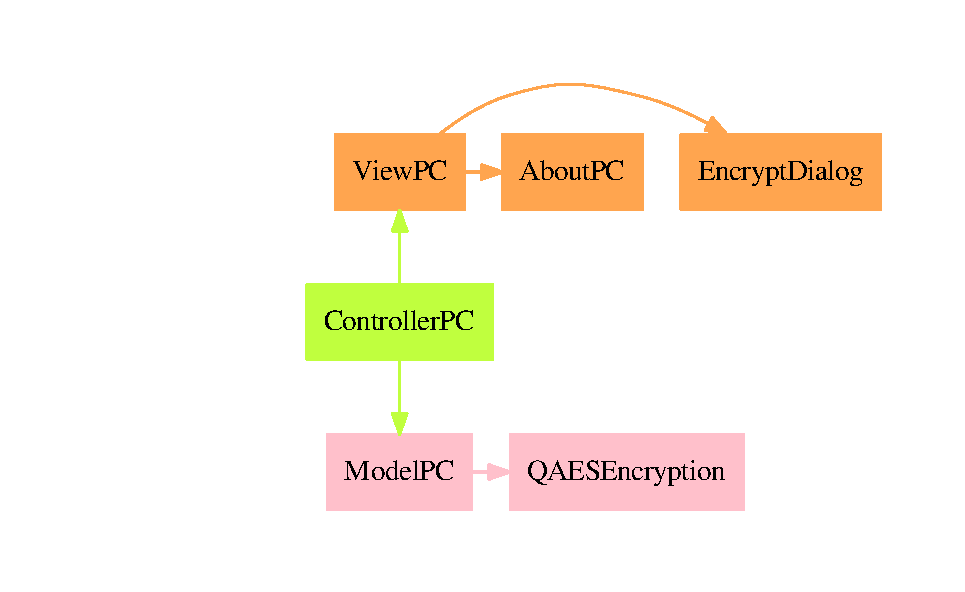
\includegraphics[width=\textwidth,height=\textheight/2,keepaspectratio=true]{dot_structure}}
\end{DoxyImageNoCaption}
\hypertarget{index_ext-use}{}\section{External use}\label{index_ext-use}
You can use \hyperlink{class_model_p_c}{Model\+PC} class separately from View and Control layer. You will need four files\+:


\begin{DoxyItemize}
\item \hyperlink{modelpc_8cpp}{modelpc.\+cpp} 
\item \hyperlink{modelpc_8h}{modelpc.\+h} 
\item \hyperlink{qaesencryption_8cpp}{aes/qaesencryption.\+cpp} 
\item \hyperlink{qaesencryption_8h}{aes/qaesencryption.\+h} 
\end{DoxyItemize}

Then you can just {\ttfamily \#include \char`\"{}modelpc.\+h\char`\"{}} and use A\+PI.\hypertarget{index_use_api}{}\subsection{A\+PI}\label{index_use_api}
Here is are the most important methods\+: 
\begin{DoxyItemize}
\item \hyperlink{class_model_p_c_a271cf9285e32df58ffbfc918e6482bbd}{Model\+P\+C\+::\+Encrypt} 
\item \hyperlink{class_model_p_c_a902abaea4f07995b48c0f2fea6eceb7c}{Model\+P\+C\+::\+Decrypt} 
\end{DoxyItemize}\hypertarget{index_Showcase}{}\subsubsection{Showcase}\label{index_Showcase}

\begin{DoxyCode}
\textcolor{comment}{// Includes}
\textcolor{preprocessor}{#include "\hyperlink{modelpc_8h}{modelpc.h}"}
\textcolor{preprocessor}{#include <QImage>}
\textcolor{preprocessor}{#include <QByteArray>}
\textcolor{preprocessor}{#include <QString>}
\textcolor{preprocessor}{#include <QDebug>} \textcolor{comment}{// just for showcase}

...

\textcolor{comment}{// Basic setup}
QByteArray data(\textcolor{stringliteral}{"some\_file.txt"});
QImage *image = \textcolor{keyword}{new} QImage(\textcolor{stringliteral}{"some\_big\_enough\_image.jpg"});
QString key = \textcolor{stringliteral}{"some\_password"};
\textcolor{keywordtype}{int} bitsUsed = 3; \textcolor{comment}{// must be from 1 to 8}

\textcolor{comment}{// Encrypting}
QString error1, error2;
QImage *normal\_resultImage = \hyperlink{class_model_p_c_a271cf9285e32df58ffbfc918e6482bbd}{ModelPC::Encrypt}(
        data,
        image,
        1,
        key,
        bitsUsed,
        &error1);
QImage *advanced\_resultImage = \hyperlink{class_model_p_c_a271cf9285e32df58ffbfc918e6482bbd}{ModelPC::Encrypt}(
        data,
        image,
        2, key,
        bitsUsed \textcolor{comment}{/* not really used here, so put here any number from 1 to 8*/},
        &error2);

\textcolor{comment}{// Decrypting with given mode}
QString error3, error4, error5, error6;
QByteArray output\_normal = \hyperlink{class_model_p_c_a902abaea4f07995b48c0f2fea6eceb7c}{ModelPC::Decrypt}(
        normal\_resultImage,
        key,
        1,
        &error3);
QByteArray output\_advanced = \hyperlink{class_model_p_c_a902abaea4f07995b48c0f2fea6eceb7c}{ModelPC::Decrypt}(
        advanced\_resultImage,
        key,
        2,
        &error4);

\textcolor{comment}{// Decrypting without given mode}
\textcolor{comment}{// PictureCrypt can detect the mode of the image and adapt.}
QByteArray output\_normal\_undefined = \hyperlink{class_model_p_c_a902abaea4f07995b48c0f2fea6eceb7c}{ModelPC::Decrypt}(
        normal\_resultImage,
        key,
        0,
        &error5);
QByteArray output\_advanced\_undefined = \hyperlink{class_model_p_c_a902abaea4f07995b48c0f2fea6eceb7c}{ModelPC::Decrypt}(
        advanced\_resultImage,
        key,
        0,
        &error6);

\textcolor{comment}{// Check (better testing with [running tests](#run-tests)}
\textcolor{keywordtype}{bool} data\_good =
        data == output\_normal &&
        data == output\_advanced &&
        data == output\_normal\_undefined &&
        data == output\_advanced\_undefined;
\textcolor{keywordtype}{bool} no\_errors =
        error1 == \textcolor{stringliteral}{"ok"} &&
        error2 == \textcolor{stringliteral}{"ok"} &&
        error3 == \textcolor{stringliteral}{"ok"} &&
        error4 == \textcolor{stringliteral}{"ok"} &&
        error5 == \textcolor{stringliteral}{"ok"} &&
        error6 == \textcolor{stringliteral}{"ok"};
\textcolor{keywordflow}{if}(data\_good && no\_errors)
    qDebug() << \textcolor{stringliteral}{"PASS"};
\textcolor{keywordflow}{else}
    qDebug() << \textcolor{stringliteral}{"FAIL"};
\end{DoxyCode}
\hypertarget{index_license}{}\section{License}\label{index_license}
This software is provided under the M\+IT License\hypertarget{index_contact}{}\section{Contact us}\label{index_contact}
Visit my site\+: \href{https://www.alexkovrigin.me}{\tt https\+://www.\+alexkovrigin.\+me}

Email me at \href{mailto:a.kovrigin0@gmail.com}{\tt a.\+kovrigin0@gmail.\+com}

\begin{DoxyAuthor}{Author}
Alexander Kovrigin (waleko) 
\end{DoxyAuthor}
\begin{DoxyCopyright}{Copyright}
Alexander Kovrigin 2019  
\end{DoxyCopyright}

\chapter{Namespace Index}
\section{Namespace List}
Here is a list of all namespaces with brief descriptions\-:\begin{DoxyCompactList}
\item\contentsline{section}{\hyperlink{namespace_errors_dict_setup}{Errors\-Dict\-Setup} }{\pageref{namespace_errors_dict_setup}}{}
\item\contentsline{section}{\hyperlink{namespace_ui}{Ui} }{\pageref{namespace_ui}}{}
\end{DoxyCompactList}

\chapter{Hierarchical Index}
\section{Class Hierarchy}
This inheritance list is sorted roughly, but not completely, alphabetically\+:\begin{DoxyCompactList}
\item Q\+Dialog\begin{DoxyCompactList}
\item \contentsline{section}{About\+PC}{\pageref{class_about_p_c}}{}
\item \contentsline{section}{Encrypt\+Dialog}{\pageref{class_encrypt_dialog}}{}
\end{DoxyCompactList}
\item Q\+Main\+Window\begin{DoxyCompactList}
\item \contentsline{section}{View\+PC}{\pageref{class_view_p_c}}{}
\end{DoxyCompactList}
\item Q\+Object\begin{DoxyCompactList}
\item \contentsline{section}{Controller\+PC}{\pageref{class_controller_p_c}}{}
\item \contentsline{section}{Model\+PC}{\pageref{class_model_p_c}}{}
\item \contentsline{section}{Q\+A\+E\+S\+Encryption}{\pageref{class_q_a_e_s_encryption}}{}
\end{DoxyCompactList}
\end{DoxyCompactList}

\chapter{Class Index}
\section{Class List}
Here are the classes, structs, unions and interfaces with brief descriptions\-:\begin{DoxyCompactList}
\item\contentsline{section}{\hyperlink{class_about_p_c}{About\-P\-C} \\*The About Page dialog }{\pageref{class_about_p_c}}{}
\item\contentsline{section}{\hyperlink{class_controller_p_c}{Controller\-P\-C} \\*The \hyperlink{class_controller_p_c}{Controller\-P\-C} class Controller class, which controls View and Model layers }{\pageref{class_controller_p_c}}{}
\item\contentsline{section}{\hyperlink{class_encrypt_dialog}{Encrypt\-Dialog} \\*Class to get the image and key to store secret info }{\pageref{class_encrypt_dialog}}{}
\item\contentsline{section}{\hyperlink{class_model_p_c}{Model\-P\-C} \\*The \hyperlink{class_model_p_c}{Model\-P\-C} class Model Layer of the app. Main class that does the work of Picture\-Crypt logic Controled by \hyperlink{class_controller_p_c}{Controller\-P\-C} }{\pageref{class_model_p_c}}{}
\item\contentsline{section}{\hyperlink{class_q_a_e_s_encryption}{Q\-A\-E\-S\-Encryption} \\*Small and portable A\-E\-S encryption class for Qt. Supports all key sizes -\/ 128/192/256 bits -\/ E\-C\-B, C\-B\-C, C\-F\-B and O\-F\-B modes. Class made entirely by bricke. Github\-: \href{https://github.com/bricke/Qt-AES}{\tt https\-://github.\-com/bricke/\-Qt-\/\-A\-E\-S} }{\pageref{class_q_a_e_s_encryption}}{}
\item\contentsline{section}{\hyperlink{class_view_p_c}{View\-P\-C} \\*View layer of the app. Controls \hyperlink{class_encrypt_dialog}{Encrypt\-Dialog} and Progress\-Dialog }{\pageref{class_view_p_c}}{}
\end{DoxyCompactList}

\chapter{File Index}
\section{File List}
Here is a list of all files with brief descriptions\+:\begin{DoxyCompactList}
\item\contentsline{section}{\hyperlink{aboutpc_8cpp}{aboutpc.\+cpp} }{\pageref{aboutpc_8cpp}}{}
\item\contentsline{section}{\hyperlink{aboutpc_8h}{aboutpc.\+h} }{\pageref{aboutpc_8h}}{}
\item\contentsline{section}{\hyperlink{controllerpc_8cpp}{controllerpc.\+cpp} }{\pageref{controllerpc_8cpp}}{}
\item\contentsline{section}{\hyperlink{controllerpc_8h}{controllerpc.\+h} }{\pageref{controllerpc_8h}}{}
\item\contentsline{section}{\hyperlink{encryptdialog_8cpp}{encryptdialog.\+cpp} }{\pageref{encryptdialog_8cpp}}{}
\item\contentsline{section}{\hyperlink{encryptdialog_8h}{encryptdialog.\+h} }{\pageref{encryptdialog_8h}}{}
\item\contentsline{section}{\hyperlink{main_8cpp}{main.\+cpp} }{\pageref{main_8cpp}}{}
\item\contentsline{section}{\hyperlink{modelpc_8cpp}{modelpc.\+cpp} }{\pageref{modelpc_8cpp}}{}
\item\contentsline{section}{\hyperlink{modelpc_8h}{modelpc.\+h} }{\pageref{modelpc_8h}}{}
\item\contentsline{section}{\hyperlink{qaesencryption_8cpp}{qaesencryption.\+cpp} }{\pageref{qaesencryption_8cpp}}{}
\item\contentsline{section}{\hyperlink{qaesencryption_8h}{qaesencryption.\+h} }{\pageref{qaesencryption_8h}}{}
\item\contentsline{section}{\hyperlink{viewpc_8cpp}{viewpc.\+cpp} }{\pageref{viewpc_8cpp}}{}
\item\contentsline{section}{\hyperlink{viewpc_8h}{viewpc.\+h} }{\pageref{viewpc_8h}}{}
\end{DoxyCompactList}

\chapter{Namespace Documentation}
\hypertarget{namespace_errors_dict_setup}{\section{Errors\-Dict\-Setup Namespace Reference}
\label{namespace_errors_dict_setup}\index{Errors\-Dict\-Setup@{Errors\-Dict\-Setup}}
}
\subsection*{Variables}
\begin{DoxyCompactItemize}
\item 
string \hyperlink{namespace_errors_dict_setup_a0c97c48fca0fdec3e730b9df1dbab9c7}{filename} = 'Errors\-Dict.\-json'
\item 
tuple \hyperlink{namespace_errors_dict_setup_ad08a9cc68898a62eb6523550f54917cf}{raw} = open(\hyperlink{namespace_errors_dict_setup_a0c97c48fca0fdec3e730b9df1dbab9c7}{filename}, 'r')
\item 
tuple \hyperlink{namespace_errors_dict_setup_adf4c30d205d29df7343e26f7c62b0685}{data} = json.\-load(\hyperlink{namespace_errors_dict_setup_ad08a9cc68898a62eb6523550f54917cf}{raw})
\item 
tuple \hyperlink{namespace_errors_dict_setup_a27081bed64a1fae4487e33cd53862a6f}{input\-\_\-data} = input()
\end{DoxyCompactItemize}


\subsection{Variable Documentation}
\hypertarget{namespace_errors_dict_setup_adf4c30d205d29df7343e26f7c62b0685}{\index{Errors\-Dict\-Setup@{Errors\-Dict\-Setup}!data@{data}}
\index{data@{data}!ErrorsDictSetup@{Errors\-Dict\-Setup}}
\subsubsection[{data}]{\setlength{\rightskip}{0pt plus 5cm}tuple Errors\-Dict\-Setup.\-data = json.\-load({\bf raw})}}\label{namespace_errors_dict_setup_adf4c30d205d29df7343e26f7c62b0685}


Definition at line \hyperlink{_errors_dict_setup_8py_source_l00006}{6} of file \hyperlink{_errors_dict_setup_8py_source}{Errors\-Dict\-Setup.\-py}.

\hypertarget{namespace_errors_dict_setup_a0c97c48fca0fdec3e730b9df1dbab9c7}{\index{Errors\-Dict\-Setup@{Errors\-Dict\-Setup}!filename@{filename}}
\index{filename@{filename}!ErrorsDictSetup@{Errors\-Dict\-Setup}}
\subsubsection[{filename}]{\setlength{\rightskip}{0pt plus 5cm}string Errors\-Dict\-Setup.\-filename = 'Errors\-Dict.\-json'}}\label{namespace_errors_dict_setup_a0c97c48fca0fdec3e730b9df1dbab9c7}


Definition at line \hyperlink{_errors_dict_setup_8py_source_l00002}{2} of file \hyperlink{_errors_dict_setup_8py_source}{Errors\-Dict\-Setup.\-py}.

\hypertarget{namespace_errors_dict_setup_a27081bed64a1fae4487e33cd53862a6f}{\index{Errors\-Dict\-Setup@{Errors\-Dict\-Setup}!input\-\_\-data@{input\-\_\-data}}
\index{input\-\_\-data@{input\-\_\-data}!ErrorsDictSetup@{Errors\-Dict\-Setup}}
\subsubsection[{input\-\_\-data}]{\setlength{\rightskip}{0pt plus 5cm}tuple Errors\-Dict\-Setup.\-input\-\_\-data = input()}}\label{namespace_errors_dict_setup_a27081bed64a1fae4487e33cd53862a6f}


Definition at line \hyperlink{_errors_dict_setup_8py_source_l00014}{14} of file \hyperlink{_errors_dict_setup_8py_source}{Errors\-Dict\-Setup.\-py}.

\hypertarget{namespace_errors_dict_setup_ad08a9cc68898a62eb6523550f54917cf}{\index{Errors\-Dict\-Setup@{Errors\-Dict\-Setup}!raw@{raw}}
\index{raw@{raw}!ErrorsDictSetup@{Errors\-Dict\-Setup}}
\subsubsection[{raw}]{\setlength{\rightskip}{0pt plus 5cm}tuple Errors\-Dict\-Setup.\-raw = open({\bf filename}, 'r')}}\label{namespace_errors_dict_setup_ad08a9cc68898a62eb6523550f54917cf}


Definition at line \hyperlink{_errors_dict_setup_8py_source_l00004}{4} of file \hyperlink{_errors_dict_setup_8py_source}{Errors\-Dict\-Setup.\-py}.


\hypertarget{namespacetests-setup}{}\section{tests-\/setup Namespace Reference}
\label{namespacetests-setup}\index{tests-\/setup@{tests-\/setup}}
\subsection*{Variables}
\begin{DoxyCompactItemize}
\item 
string \mbox{\hyperlink{namespacetests-setup_a1c1b6d4c14026d664106586c65e10a94}{filename}} = \textquotesingle{}tests.\+json\textquotesingle{}
\item 
\mbox{\hyperlink{namespacetests-setup_a16d40f6dd9430f3bdc79db2d00aab267}{raw}} = open(\mbox{\hyperlink{namespacetests-setup_a1c1b6d4c14026d664106586c65e10a94}{filename}}, \textquotesingle{}r\textquotesingle{})
\item 
\mbox{\hyperlink{namespacetests-setup_a94275a2f2d070d13dedc7e8dfaf4faa0}{js}} = json.\+load(\mbox{\hyperlink{namespacetests-setup_a16d40f6dd9430f3bdc79db2d00aab267}{raw}})
\item 
\mbox{\hyperlink{namespacetests-setup_a92ab4d3dccd0fc5347ed0f5399869803}{sep}}
\item 
\mbox{\hyperlink{namespacetests-setup_a1e5de3b19e0107100d5df9b7e2122764}{input\+\_\+data}} = input()
\item 
list \mbox{\hyperlink{namespacetests-setup_a274aaa7c0d5733ef5f48372d9481f34a}{arr}} = \mbox{[}$\,$\mbox{]}
\item 
\mbox{\hyperlink{namespacetests-setup_a6b4da66e7d24a18856de9023a2dcede4}{data}}
\item 
\mbox{\hyperlink{namespacetests-setup_ad55b685280f549e15688a94cbb89f512}{image}}
\item 
\mbox{\hyperlink{namespacetests-setup_a2c17344dec99b9aaaddaef4438b1f793}{expect}}
\item 
\mbox{\hyperlink{namespacetests-setup_a04126d10edec6b3171e1b55a00309b23}{mode}}
\item 
\mbox{\hyperlink{namespacetests-setup_a3a21e3298c630c17fc27ca5ab146a8af}{key}}
\item 
\mbox{\hyperlink{namespacetests-setup_a64974eb034f518d24195739395783d3d}{bits\+Used}}
\item 
dictionary \mbox{\hyperlink{namespacetests-setup_afb80c1236926b5468a6d3e942a527a96}{obj}} = \{\textquotesingle{}\mbox{\hyperlink{namespacetests-setup_a6b4da66e7d24a18856de9023a2dcede4}{data}}\textquotesingle{}\+:\mbox{\hyperlink{namespacetests-setup_a6b4da66e7d24a18856de9023a2dcede4}{data}}, \textquotesingle{}\mbox{\hyperlink{namespacetests-setup_ad55b685280f549e15688a94cbb89f512}{image}}\textquotesingle{}\+:\mbox{\hyperlink{namespacetests-setup_ad55b685280f549e15688a94cbb89f512}{image}},\textquotesingle{}expectation\textquotesingle{}\+:\mbox{\hyperlink{namespacetests-setup_a2c17344dec99b9aaaddaef4438b1f793}{expect}},\textquotesingle{}\mbox{\hyperlink{namespacetests-setup_a04126d10edec6b3171e1b55a00309b23}{mode}}\textquotesingle{}\+:int(\mbox{\hyperlink{namespacetests-setup_a04126d10edec6b3171e1b55a00309b23}{mode}}),\textquotesingle{}\mbox{\hyperlink{namespacetests-setup_a3a21e3298c630c17fc27ca5ab146a8af}{key}}\textquotesingle{}\+:\mbox{\hyperlink{namespacetests-setup_a3a21e3298c630c17fc27ca5ab146a8af}{key}},\textquotesingle{}\mbox{\hyperlink{namespacetests-setup_a64974eb034f518d24195739395783d3d}{bits\+Used}}\textquotesingle{}\+:int(\mbox{\hyperlink{namespacetests-setup_a64974eb034f518d24195739395783d3d}{bits\+Used}})\}
\item 
\mbox{\hyperlink{namespacetests-setup_a919f85fdaaec93d91baf4a46863c31fd}{f}}
\item 
\mbox{\hyperlink{namespacetests-setup_aee04695e456c1d05ed5119e87842fc86}{indent}}
\end{DoxyCompactItemize}


\subsection{Variable Documentation}
\mbox{\Hypertarget{namespacetests-setup_a274aaa7c0d5733ef5f48372d9481f34a}\label{namespacetests-setup_a274aaa7c0d5733ef5f48372d9481f34a}} 
\index{tests-\/setup@{tests-\/setup}!arr@{arr}}
\index{arr@{arr}!tests-\/setup@{tests-\/setup}}
\subsubsection{\texorpdfstring{arr}{arr}}
{\footnotesize\ttfamily list tests-\/setup.\+arr = \mbox{[}$\,$\mbox{]}}



Definition at line \mbox{\hyperlink{tests-setup_8py_source_l00016}{16}} of file \mbox{\hyperlink{tests-setup_8py_source}{tests-\/setup.\+py}}.

\mbox{\Hypertarget{namespacetests-setup_a64974eb034f518d24195739395783d3d}\label{namespacetests-setup_a64974eb034f518d24195739395783d3d}} 
\index{tests-\/setup@{tests-\/setup}!bits\+Used@{bits\+Used}}
\index{bits\+Used@{bits\+Used}!tests-\/setup@{tests-\/setup}}
\subsubsection{\texorpdfstring{bits\+Used}{bitsUsed}}
{\footnotesize\ttfamily tests-\/setup.\+bits\+Used}



Definition at line \mbox{\hyperlink{tests-setup_8py_source_l00018}{18}} of file \mbox{\hyperlink{tests-setup_8py_source}{tests-\/setup.\+py}}.

\mbox{\Hypertarget{namespacetests-setup_a6b4da66e7d24a18856de9023a2dcede4}\label{namespacetests-setup_a6b4da66e7d24a18856de9023a2dcede4}} 
\index{tests-\/setup@{tests-\/setup}!data@{data}}
\index{data@{data}!tests-\/setup@{tests-\/setup}}
\subsubsection{\texorpdfstring{data}{data}}
{\footnotesize\ttfamily tests-\/setup.\+data}



Definition at line \mbox{\hyperlink{tests-setup_8py_source_l00018}{18}} of file \mbox{\hyperlink{tests-setup_8py_source}{tests-\/setup.\+py}}.

\mbox{\Hypertarget{namespacetests-setup_a2c17344dec99b9aaaddaef4438b1f793}\label{namespacetests-setup_a2c17344dec99b9aaaddaef4438b1f793}} 
\index{tests-\/setup@{tests-\/setup}!expect@{expect}}
\index{expect@{expect}!tests-\/setup@{tests-\/setup}}
\subsubsection{\texorpdfstring{expect}{expect}}
{\footnotesize\ttfamily tests-\/setup.\+expect}



Definition at line \mbox{\hyperlink{tests-setup_8py_source_l00018}{18}} of file \mbox{\hyperlink{tests-setup_8py_source}{tests-\/setup.\+py}}.

\mbox{\Hypertarget{namespacetests-setup_a919f85fdaaec93d91baf4a46863c31fd}\label{namespacetests-setup_a919f85fdaaec93d91baf4a46863c31fd}} 
\index{tests-\/setup@{tests-\/setup}!f@{f}}
\index{f@{f}!tests-\/setup@{tests-\/setup}}
\subsubsection{\texorpdfstring{f}{f}}
{\footnotesize\ttfamily tests-\/setup.\+f}



Definition at line \mbox{\hyperlink{tests-setup_8py_source_l00026}{26}} of file \mbox{\hyperlink{tests-setup_8py_source}{tests-\/setup.\+py}}.

\mbox{\Hypertarget{namespacetests-setup_a1c1b6d4c14026d664106586c65e10a94}\label{namespacetests-setup_a1c1b6d4c14026d664106586c65e10a94}} 
\index{tests-\/setup@{tests-\/setup}!filename@{filename}}
\index{filename@{filename}!tests-\/setup@{tests-\/setup}}
\subsubsection{\texorpdfstring{filename}{filename}}
{\footnotesize\ttfamily string tests-\/setup.\+filename = \textquotesingle{}tests.\+json\textquotesingle{}}



Definition at line \mbox{\hyperlink{tests-setup_8py_source_l00002}{2}} of file \mbox{\hyperlink{tests-setup_8py_source}{tests-\/setup.\+py}}.

\mbox{\Hypertarget{namespacetests-setup_ad55b685280f549e15688a94cbb89f512}\label{namespacetests-setup_ad55b685280f549e15688a94cbb89f512}} 
\index{tests-\/setup@{tests-\/setup}!image@{image}}
\index{image@{image}!tests-\/setup@{tests-\/setup}}
\subsubsection{\texorpdfstring{image}{image}}
{\footnotesize\ttfamily tests-\/setup.\+image}



Definition at line \mbox{\hyperlink{tests-setup_8py_source_l00018}{18}} of file \mbox{\hyperlink{tests-setup_8py_source}{tests-\/setup.\+py}}.

\mbox{\Hypertarget{namespacetests-setup_aee04695e456c1d05ed5119e87842fc86}\label{namespacetests-setup_aee04695e456c1d05ed5119e87842fc86}} 
\index{tests-\/setup@{tests-\/setup}!indent@{indent}}
\index{indent@{indent}!tests-\/setup@{tests-\/setup}}
\subsubsection{\texorpdfstring{indent}{indent}}
{\footnotesize\ttfamily tests-\/setup.\+indent}



Definition at line \mbox{\hyperlink{tests-setup_8py_source_l00026}{26}} of file \mbox{\hyperlink{tests-setup_8py_source}{tests-\/setup.\+py}}.

\mbox{\Hypertarget{namespacetests-setup_a1e5de3b19e0107100d5df9b7e2122764}\label{namespacetests-setup_a1e5de3b19e0107100d5df9b7e2122764}} 
\index{tests-\/setup@{tests-\/setup}!input\+\_\+data@{input\+\_\+data}}
\index{input\+\_\+data@{input\+\_\+data}!tests-\/setup@{tests-\/setup}}
\subsubsection{\texorpdfstring{input\+\_\+data}{input\_data}}
{\footnotesize\ttfamily tests-\/setup.\+input\+\_\+data = input()}



Definition at line \mbox{\hyperlink{tests-setup_8py_source_l00014}{14}} of file \mbox{\hyperlink{tests-setup_8py_source}{tests-\/setup.\+py}}.

\mbox{\Hypertarget{namespacetests-setup_a94275a2f2d070d13dedc7e8dfaf4faa0}\label{namespacetests-setup_a94275a2f2d070d13dedc7e8dfaf4faa0}} 
\index{tests-\/setup@{tests-\/setup}!js@{js}}
\index{js@{js}!tests-\/setup@{tests-\/setup}}
\subsubsection{\texorpdfstring{js}{js}}
{\footnotesize\ttfamily tests-\/setup.\+js = json.\+load(\mbox{\hyperlink{namespacetests-setup_a16d40f6dd9430f3bdc79db2d00aab267}{raw}})}



Definition at line \mbox{\hyperlink{tests-setup_8py_source_l00006}{6}} of file \mbox{\hyperlink{tests-setup_8py_source}{tests-\/setup.\+py}}.

\mbox{\Hypertarget{namespacetests-setup_a3a21e3298c630c17fc27ca5ab146a8af}\label{namespacetests-setup_a3a21e3298c630c17fc27ca5ab146a8af}} 
\index{tests-\/setup@{tests-\/setup}!key@{key}}
\index{key@{key}!tests-\/setup@{tests-\/setup}}
\subsubsection{\texorpdfstring{key}{key}}
{\footnotesize\ttfamily tests-\/setup.\+key}



Definition at line \mbox{\hyperlink{tests-setup_8py_source_l00018}{18}} of file \mbox{\hyperlink{tests-setup_8py_source}{tests-\/setup.\+py}}.

\mbox{\Hypertarget{namespacetests-setup_a04126d10edec6b3171e1b55a00309b23}\label{namespacetests-setup_a04126d10edec6b3171e1b55a00309b23}} 
\index{tests-\/setup@{tests-\/setup}!mode@{mode}}
\index{mode@{mode}!tests-\/setup@{tests-\/setup}}
\subsubsection{\texorpdfstring{mode}{mode}}
{\footnotesize\ttfamily tests-\/setup.\+mode}



Definition at line \mbox{\hyperlink{tests-setup_8py_source_l00018}{18}} of file \mbox{\hyperlink{tests-setup_8py_source}{tests-\/setup.\+py}}.

\mbox{\Hypertarget{namespacetests-setup_afb80c1236926b5468a6d3e942a527a96}\label{namespacetests-setup_afb80c1236926b5468a6d3e942a527a96}} 
\index{tests-\/setup@{tests-\/setup}!obj@{obj}}
\index{obj@{obj}!tests-\/setup@{tests-\/setup}}
\subsubsection{\texorpdfstring{obj}{obj}}
{\footnotesize\ttfamily dictionary tests-\/setup.\+obj = \{\textquotesingle{}\mbox{\hyperlink{namespacetests-setup_a6b4da66e7d24a18856de9023a2dcede4}{data}}\textquotesingle{}\+:\mbox{\hyperlink{namespacetests-setup_a6b4da66e7d24a18856de9023a2dcede4}{data}}, \textquotesingle{}\mbox{\hyperlink{namespacetests-setup_ad55b685280f549e15688a94cbb89f512}{image}}\textquotesingle{}\+:\mbox{\hyperlink{namespacetests-setup_ad55b685280f549e15688a94cbb89f512}{image}},\textquotesingle{}expectation\textquotesingle{}\+:\mbox{\hyperlink{namespacetests-setup_a2c17344dec99b9aaaddaef4438b1f793}{expect}},\textquotesingle{}\mbox{\hyperlink{namespacetests-setup_a04126d10edec6b3171e1b55a00309b23}{mode}}\textquotesingle{}\+:int(\mbox{\hyperlink{namespacetests-setup_a04126d10edec6b3171e1b55a00309b23}{mode}}),\textquotesingle{}\mbox{\hyperlink{namespacetests-setup_a3a21e3298c630c17fc27ca5ab146a8af}{key}}\textquotesingle{}\+:\mbox{\hyperlink{namespacetests-setup_a3a21e3298c630c17fc27ca5ab146a8af}{key}},\textquotesingle{}\mbox{\hyperlink{namespacetests-setup_a64974eb034f518d24195739395783d3d}{bits\+Used}}\textquotesingle{}\+:int(\mbox{\hyperlink{namespacetests-setup_a64974eb034f518d24195739395783d3d}{bits\+Used}})\}}



Definition at line \mbox{\hyperlink{tests-setup_8py_source_l00020}{20}} of file \mbox{\hyperlink{tests-setup_8py_source}{tests-\/setup.\+py}}.

\mbox{\Hypertarget{namespacetests-setup_a16d40f6dd9430f3bdc79db2d00aab267}\label{namespacetests-setup_a16d40f6dd9430f3bdc79db2d00aab267}} 
\index{tests-\/setup@{tests-\/setup}!raw@{raw}}
\index{raw@{raw}!tests-\/setup@{tests-\/setup}}
\subsubsection{\texorpdfstring{raw}{raw}}
{\footnotesize\ttfamily tests-\/setup.\+raw = open(\mbox{\hyperlink{namespacetests-setup_a1c1b6d4c14026d664106586c65e10a94}{filename}}, \textquotesingle{}r\textquotesingle{})}



Definition at line \mbox{\hyperlink{tests-setup_8py_source_l00004}{4}} of file \mbox{\hyperlink{tests-setup_8py_source}{tests-\/setup.\+py}}.

\mbox{\Hypertarget{namespacetests-setup_a92ab4d3dccd0fc5347ed0f5399869803}\label{namespacetests-setup_a92ab4d3dccd0fc5347ed0f5399869803}} 
\index{tests-\/setup@{tests-\/setup}!sep@{sep}}
\index{sep@{sep}!tests-\/setup@{tests-\/setup}}
\subsubsection{\texorpdfstring{sep}{sep}}
{\footnotesize\ttfamily tests-\/setup.\+sep}



Definition at line \mbox{\hyperlink{tests-setup_8py_source_l00009}{9}} of file \mbox{\hyperlink{tests-setup_8py_source}{tests-\/setup.\+py}}.


\hypertarget{namespace_ui}{\section{Ui Namespace Reference}
\label{namespace_ui}\index{Ui@{Ui}}
}

\chapter{Class Documentation}
\hypertarget{class_about_p_c}{}\section{About\+PC Class Reference}
\label{class_about_p_c}\index{About\+PC@{About\+PC}}


The \mbox{\hyperlink{class_about_p_c}{About\+PC}} class The About Page dialog.  




{\ttfamily \#include $<$aboutpc.\+h$>$}



Inheritance diagram for About\+PC\+:
\nopagebreak
\begin{figure}[H]
\begin{center}
\leavevmode
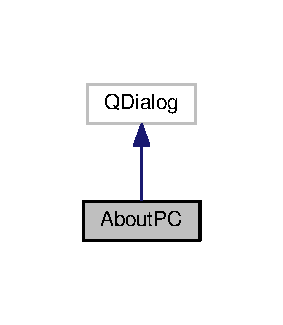
\includegraphics[width=136pt]{class_about_p_c__inherit__graph}
\end{center}
\end{figure}


Collaboration diagram for About\+PC\+:
\nopagebreak
\begin{figure}[H]
\begin{center}
\leavevmode
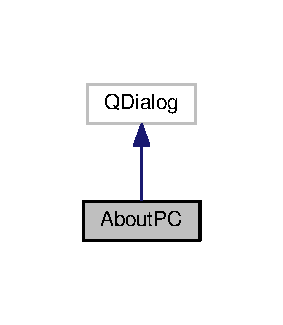
\includegraphics[width=136pt]{class_about_p_c__coll__graph}
\end{center}
\end{figure}
\subsection*{Public Member Functions}
\begin{DoxyCompactItemize}
\item 
\mbox{\hyperlink{class_about_p_c_a89341c4427d97da60acf15dc929ad8a6}{About\+PC}} (Q\+Widget $\ast$parent=0)
\item 
\mbox{\hyperlink{class_about_p_c_a3cc0c4c81abc640d946003b078a47dd4}{$\sim$\+About\+PC}} ()
\item 
void \mbox{\hyperlink{class_about_p_c_aa3815d4826d0c8d87122449537a0a4d5}{set\+Version}} (Q\+String version)
\begin{DoxyCompactList}\small\item\em \mbox{\hyperlink{class_about_p_c_aa3815d4826d0c8d87122449537a0a4d5}{About\+P\+C\+::set\+Version}} Function to set the version display. \end{DoxyCompactList}\end{DoxyCompactItemize}


\subsection{Detailed Description}
The \mbox{\hyperlink{class_about_p_c}{About\+PC}} class The About Page dialog. 

Definition at line \mbox{\hyperlink{aboutpc_8h_source_l00012}{12}} of file \mbox{\hyperlink{aboutpc_8h_source}{aboutpc.\+h}}.



\subsection{Constructor \& Destructor Documentation}
\mbox{\Hypertarget{class_about_p_c_a89341c4427d97da60acf15dc929ad8a6}\label{class_about_p_c_a89341c4427d97da60acf15dc929ad8a6}} 
\index{About\+PC@{About\+PC}!About\+PC@{About\+PC}}
\index{About\+PC@{About\+PC}!About\+PC@{About\+PC}}
\subsubsection{\texorpdfstring{About\+P\+C()}{AboutPC()}}
{\footnotesize\ttfamily About\+P\+C\+::\+About\+PC (\begin{DoxyParamCaption}\item[{Q\+Widget $\ast$}]{parent = {\ttfamily 0} }\end{DoxyParamCaption})\hspace{0.3cm}{\ttfamily [explicit]}}



Definition at line \mbox{\hyperlink{aboutpc_8cpp_source_l00004}{4}} of file \mbox{\hyperlink{aboutpc_8cpp_source}{aboutpc.\+cpp}}.

\mbox{\Hypertarget{class_about_p_c_a3cc0c4c81abc640d946003b078a47dd4}\label{class_about_p_c_a3cc0c4c81abc640d946003b078a47dd4}} 
\index{About\+PC@{About\+PC}!````~About\+PC@{$\sim$\+About\+PC}}
\index{````~About\+PC@{$\sim$\+About\+PC}!About\+PC@{About\+PC}}
\subsubsection{\texorpdfstring{$\sim$\+About\+P\+C()}{~AboutPC()}}
{\footnotesize\ttfamily About\+P\+C\+::$\sim$\+About\+PC (\begin{DoxyParamCaption}{ }\end{DoxyParamCaption})}



Definition at line \mbox{\hyperlink{aboutpc_8cpp_source_l00011}{11}} of file \mbox{\hyperlink{aboutpc_8cpp_source}{aboutpc.\+cpp}}.



\subsection{Member Function Documentation}
\mbox{\Hypertarget{class_about_p_c_aa3815d4826d0c8d87122449537a0a4d5}\label{class_about_p_c_aa3815d4826d0c8d87122449537a0a4d5}} 
\index{About\+PC@{About\+PC}!set\+Version@{set\+Version}}
\index{set\+Version@{set\+Version}!About\+PC@{About\+PC}}
\subsubsection{\texorpdfstring{set\+Version()}{setVersion()}}
{\footnotesize\ttfamily void About\+P\+C\+::set\+Version (\begin{DoxyParamCaption}\item[{Q\+String}]{version }\end{DoxyParamCaption})}



\mbox{\hyperlink{class_about_p_c_aa3815d4826d0c8d87122449537a0a4d5}{About\+P\+C\+::set\+Version}} Function to set the version display. 


\begin{DoxyParams}{Parameters}
{\em version} & Version as Q\+String \\
\hline
\end{DoxyParams}


Definition at line \mbox{\hyperlink{aboutpc_8cpp_source_l00019}{19}} of file \mbox{\hyperlink{aboutpc_8cpp_source}{aboutpc.\+cpp}}.

Here is the caller graph for this function\+:
\nopagebreak
\begin{figure}[H]
\begin{center}
\leavevmode
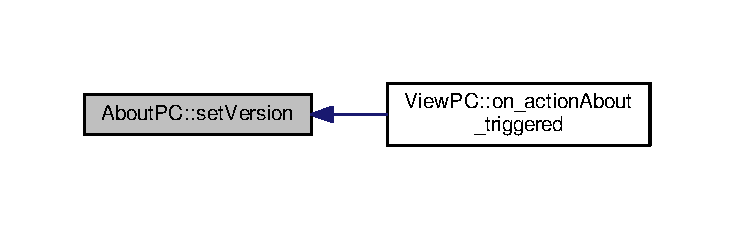
\includegraphics[width=349pt]{class_about_p_c_aa3815d4826d0c8d87122449537a0a4d5_icgraph}
\end{center}
\end{figure}


The documentation for this class was generated from the following files\+:\begin{DoxyCompactItemize}
\item 
C\+:/\+Users/salex/\+Documents/\+Git\+Hub/\+Picture\+Crypt/src/\mbox{\hyperlink{aboutpc_8h}{aboutpc.\+h}}\item 
C\+:/\+Users/salex/\+Documents/\+Git\+Hub/\+Picture\+Crypt/src/\mbox{\hyperlink{aboutpc_8cpp}{aboutpc.\+cpp}}\end{DoxyCompactItemize}

\hypertarget{class_controller_p_c}{}\section{Controller\+PC Class Reference}
\label{class_controller_p_c}\index{Controller\+PC@{Controller\+PC}}


The \mbox{\hyperlink{class_controller_p_c}{Controller\+PC}} class Controller class, which controls View and Model layers.  




{\ttfamily \#include $<$controllerpc.\+h$>$}



Inheritance diagram for Controller\+PC\+:
\nopagebreak
\begin{figure}[H]
\begin{center}
\leavevmode
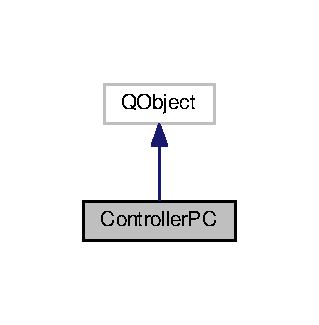
\includegraphics[width=151pt]{class_controller_p_c__inherit__graph}
\end{center}
\end{figure}


Collaboration diagram for Controller\+PC\+:
\nopagebreak
\begin{figure}[H]
\begin{center}
\leavevmode
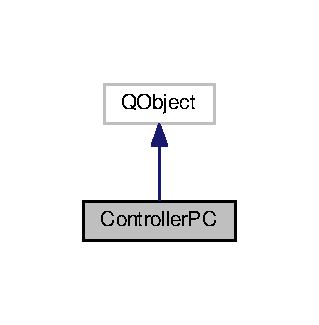
\includegraphics[width=151pt]{class_controller_p_c__coll__graph}
\end{center}
\end{figure}
\subsection*{Public Slots}
\begin{DoxyCompactItemize}
\item 
void \mbox{\hyperlink{class_controller_p_c_a8814989f7be1214e06b2e720889066b0}{abort\+Circuit}} ()
\begin{DoxyCompactList}\small\item\em \mbox{\hyperlink{class_controller_p_c_a8814989f7be1214e06b2e720889066b0}{Controller\+P\+C\+::abort\+Circuit}} Slot to be called when Progress\+Dialog in \mbox{\hyperlink{class_view_p_c}{View\+PC}} is closed. It flags \mbox{\hyperlink{class_model_p_c}{Model\+PC}} to stop. \end{DoxyCompactList}\item 
void \mbox{\hyperlink{class_controller_p_c_afd8d33ed84e463c5e0ce6715067003f3}{set\+Bits\+Used}} (int bits\+Used)
\begin{DoxyCompactList}\small\item\em \mbox{\hyperlink{class_controller_p_c_afd8d33ed84e463c5e0ce6715067003f3}{Controller\+P\+C\+::set\+Bits\+Used}} Slot to set \mbox{\hyperlink{class_model_p_c_a655deb6a8afa94c7f4aadb3056989038}{Model\+P\+C\+::bits\+Used}}. \end{DoxyCompactList}\item 
void \mbox{\hyperlink{class_controller_p_c_ac00d29685a7e5b780c01eb438e10f96d}{set\+J\+P\+H\+S\+Dir}} (Q\+String dir)
\begin{DoxyCompactList}\small\item\em \mbox{\hyperlink{class_controller_p_c_ac00d29685a7e5b780c01eb438e10f96d}{Controller\+P\+C\+::set\+J\+P\+H\+S\+Dir}} Sets J\+P\+HS default dir. \end{DoxyCompactList}\end{DoxyCompactItemize}
\subsection*{Public Member Functions}
\begin{DoxyCompactItemize}
\item 
\mbox{\hyperlink{class_controller_p_c_afa6c92d67bf3b6531c42385fc5938003}{Controller\+PC}} ()
\begin{DoxyCompactList}\small\item\em \mbox{\hyperlink{class_controller_p_c_afa6c92d67bf3b6531c42385fc5938003}{Controller\+P\+C\+::\+Controller\+PC}} Constructor of controller Constructor runs auto-\/test for \mbox{\hyperlink{class_model_p_c}{Model\+PC}}, creates Model Class (\mbox{\hyperlink{class_model_p_c}{Model\+PC}}) and View Class (\mbox{\hyperlink{class_view_p_c}{View\+PC}}). All signals and slots are connected here. \end{DoxyCompactList}\end{DoxyCompactItemize}
\subsection*{Public Attributes}
\begin{DoxyCompactItemize}
\item 
long int \mbox{\hyperlink{class_controller_p_c_a9eb43c34237d66751a6411e55cf5f55e}{version}}
\begin{DoxyCompactList}\small\item\em version Version of the app \end{DoxyCompactList}\item 
Q\+String \mbox{\hyperlink{class_controller_p_c_a0e63cca37d6ce2e660f3380400c2c5f3}{version\+String}}
\begin{DoxyCompactList}\small\item\em version\+String Version of the app as Q\+String. \end{DoxyCompactList}\end{DoxyCompactItemize}


\subsection{Detailed Description}
The \mbox{\hyperlink{class_controller_p_c}{Controller\+PC}} class Controller class, which controls View and Model layers. 

\begin{DoxySeeAlso}{See also}
\mbox{\hyperlink{class_view_p_c}{View\+PC}}, \mbox{\hyperlink{class_model_p_c}{Model\+PC}} 
\end{DoxySeeAlso}


Definition at line \mbox{\hyperlink{controllerpc_8h_source_l00019}{19}} of file \mbox{\hyperlink{controllerpc_8h_source}{controllerpc.\+h}}.



\subsection{Constructor \& Destructor Documentation}
\mbox{\Hypertarget{class_controller_p_c_afa6c92d67bf3b6531c42385fc5938003}\label{class_controller_p_c_afa6c92d67bf3b6531c42385fc5938003}} 
\index{Controller\+PC@{Controller\+PC}!Controller\+PC@{Controller\+PC}}
\index{Controller\+PC@{Controller\+PC}!Controller\+PC@{Controller\+PC}}
\subsubsection{\texorpdfstring{Controller\+P\+C()}{ControllerPC()}}
{\footnotesize\ttfamily Controller\+P\+C\+::\+Controller\+PC (\begin{DoxyParamCaption}{ }\end{DoxyParamCaption})}



\mbox{\hyperlink{class_controller_p_c_afa6c92d67bf3b6531c42385fc5938003}{Controller\+P\+C\+::\+Controller\+PC}} Constructor of controller Constructor runs auto-\/test for \mbox{\hyperlink{class_model_p_c}{Model\+PC}}, creates Model Class (\mbox{\hyperlink{class_model_p_c}{Model\+PC}}) and View Class (\mbox{\hyperlink{class_view_p_c}{View\+PC}}). All signals and slots are connected here. 

Controller class \begin{DoxyNote}{Note}
Version of the app is specified here. 
\end{DoxyNote}


Definition at line \mbox{\hyperlink{controllerpc_8cpp_source_l00009}{9}} of file \mbox{\hyperlink{controllerpc_8cpp_source}{controllerpc.\+cpp}}.

Here is the call graph for this function\+:
\nopagebreak
\begin{figure}[H]
\begin{center}
\leavevmode
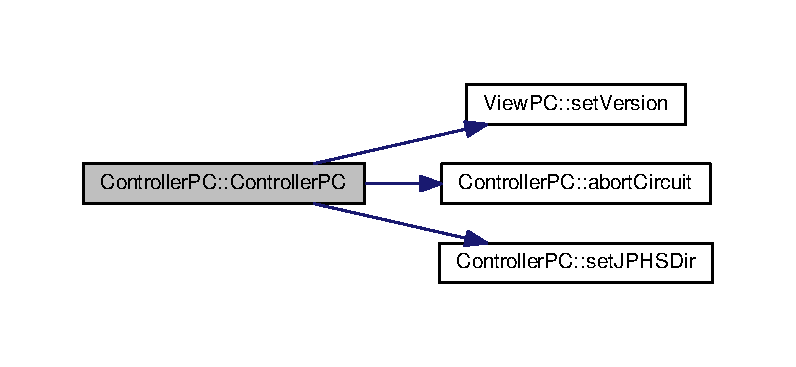
\includegraphics[width=350pt]{class_controller_p_c_afa6c92d67bf3b6531c42385fc5938003_cgraph}
\end{center}
\end{figure}


\subsection{Member Function Documentation}
\mbox{\Hypertarget{class_controller_p_c_a8814989f7be1214e06b2e720889066b0}\label{class_controller_p_c_a8814989f7be1214e06b2e720889066b0}} 
\index{Controller\+PC@{Controller\+PC}!abort\+Circuit@{abort\+Circuit}}
\index{abort\+Circuit@{abort\+Circuit}!Controller\+PC@{Controller\+PC}}
\subsubsection{\texorpdfstring{abort\+Circuit}{abortCircuit}}
{\footnotesize\ttfamily void Controller\+P\+C\+::abort\+Circuit (\begin{DoxyParamCaption}{ }\end{DoxyParamCaption})\hspace{0.3cm}{\ttfamily [slot]}}



\mbox{\hyperlink{class_controller_p_c_a8814989f7be1214e06b2e720889066b0}{Controller\+P\+C\+::abort\+Circuit}} Slot to be called when Progress\+Dialog in \mbox{\hyperlink{class_view_p_c}{View\+PC}} is closed. It flags \mbox{\hyperlink{class_model_p_c}{Model\+PC}} to stop. 



Definition at line \mbox{\hyperlink{controllerpc_8cpp_source_l00036}{36}} of file \mbox{\hyperlink{controllerpc_8cpp_source}{controllerpc.\+cpp}}.

Here is the caller graph for this function\+:
\nopagebreak
\begin{figure}[H]
\begin{center}
\leavevmode
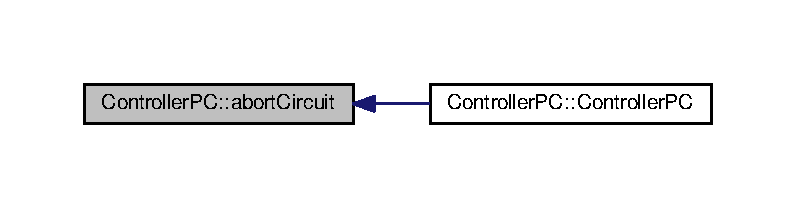
\includegraphics[width=350pt]{class_controller_p_c_a8814989f7be1214e06b2e720889066b0_icgraph}
\end{center}
\end{figure}
\mbox{\Hypertarget{class_controller_p_c_afd8d33ed84e463c5e0ce6715067003f3}\label{class_controller_p_c_afd8d33ed84e463c5e0ce6715067003f3}} 
\index{Controller\+PC@{Controller\+PC}!set\+Bits\+Used@{set\+Bits\+Used}}
\index{set\+Bits\+Used@{set\+Bits\+Used}!Controller\+PC@{Controller\+PC}}
\subsubsection{\texorpdfstring{set\+Bits\+Used}{setBitsUsed}}
{\footnotesize\ttfamily void Controller\+P\+C\+::set\+Bits\+Used (\begin{DoxyParamCaption}\item[{int}]{bits\+Used }\end{DoxyParamCaption})\hspace{0.3cm}{\ttfamily [slot]}}



\mbox{\hyperlink{class_controller_p_c_afd8d33ed84e463c5e0ce6715067003f3}{Controller\+P\+C\+::set\+Bits\+Used}} Slot to set \mbox{\hyperlink{class_model_p_c_a655deb6a8afa94c7f4aadb3056989038}{Model\+P\+C\+::bits\+Used}}. 


\begin{DoxyParams}{Parameters}
{\em bits\+Used} & Value \\
\hline
\end{DoxyParams}


Definition at line \mbox{\hyperlink{controllerpc_8cpp_source_l00044}{44}} of file \mbox{\hyperlink{controllerpc_8cpp_source}{controllerpc.\+cpp}}.

Here is the caller graph for this function\+:
\nopagebreak
\begin{figure}[H]
\begin{center}
\leavevmode
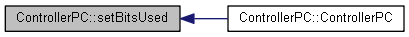
\includegraphics[width=350pt]{class_controller_p_c_afd8d33ed84e463c5e0ce6715067003f3_icgraph}
\end{center}
\end{figure}
\mbox{\Hypertarget{class_controller_p_c_ac00d29685a7e5b780c01eb438e10f96d}\label{class_controller_p_c_ac00d29685a7e5b780c01eb438e10f96d}} 
\index{Controller\+PC@{Controller\+PC}!set\+J\+P\+H\+S\+Dir@{set\+J\+P\+H\+S\+Dir}}
\index{set\+J\+P\+H\+S\+Dir@{set\+J\+P\+H\+S\+Dir}!Controller\+PC@{Controller\+PC}}
\subsubsection{\texorpdfstring{set\+J\+P\+H\+S\+Dir}{setJPHSDir}}
{\footnotesize\ttfamily void Controller\+P\+C\+::set\+J\+P\+H\+S\+Dir (\begin{DoxyParamCaption}\item[{Q\+String}]{dir }\end{DoxyParamCaption})\hspace{0.3cm}{\ttfamily [slot]}}



\mbox{\hyperlink{class_controller_p_c_ac00d29685a7e5b780c01eb438e10f96d}{Controller\+P\+C\+::set\+J\+P\+H\+S\+Dir}} Sets J\+P\+HS default dir. 


\begin{DoxyParams}{Parameters}
{\em dir} & Directory \\
\hline
\end{DoxyParams}


Definition at line \mbox{\hyperlink{controllerpc_8cpp_source_l00052}{52}} of file \mbox{\hyperlink{controllerpc_8cpp_source}{controllerpc.\+cpp}}.

Here is the caller graph for this function\+:
\nopagebreak
\begin{figure}[H]
\begin{center}
\leavevmode
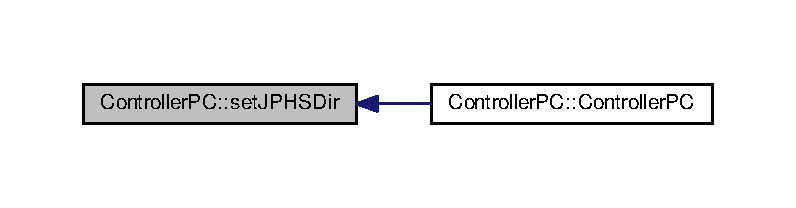
\includegraphics[width=350pt]{class_controller_p_c_ac00d29685a7e5b780c01eb438e10f96d_icgraph}
\end{center}
\end{figure}


\subsection{Member Data Documentation}
\mbox{\Hypertarget{class_controller_p_c_a9eb43c34237d66751a6411e55cf5f55e}\label{class_controller_p_c_a9eb43c34237d66751a6411e55cf5f55e}} 
\index{Controller\+PC@{Controller\+PC}!version@{version}}
\index{version@{version}!Controller\+PC@{Controller\+PC}}
\subsubsection{\texorpdfstring{version}{version}}
{\footnotesize\ttfamily long int Controller\+P\+C\+::version}



version Version of the app 



Definition at line \mbox{\hyperlink{controllerpc_8h_source_l00027}{27}} of file \mbox{\hyperlink{controllerpc_8h_source}{controllerpc.\+h}}.

\mbox{\Hypertarget{class_controller_p_c_a0e63cca37d6ce2e660f3380400c2c5f3}\label{class_controller_p_c_a0e63cca37d6ce2e660f3380400c2c5f3}} 
\index{Controller\+PC@{Controller\+PC}!version\+String@{version\+String}}
\index{version\+String@{version\+String}!Controller\+PC@{Controller\+PC}}
\subsubsection{\texorpdfstring{version\+String}{versionString}}
{\footnotesize\ttfamily Q\+String Controller\+P\+C\+::version\+String}



version\+String Version of the app as Q\+String. 



Definition at line \mbox{\hyperlink{controllerpc_8h_source_l00031}{31}} of file \mbox{\hyperlink{controllerpc_8h_source}{controllerpc.\+h}}.



The documentation for this class was generated from the following files\+:\begin{DoxyCompactItemize}
\item 
C\+:/\+Users/salex/\+Documents/\+Git\+Hub/\+Picture\+Crypt/\mbox{\hyperlink{controllerpc_8h}{controllerpc.\+h}}\item 
C\+:/\+Users/salex/\+Documents/\+Git\+Hub/\+Picture\+Crypt/\mbox{\hyperlink{controllerpc_8cpp}{controllerpc.\+cpp}}\end{DoxyCompactItemize}

\hypertarget{class_encrypt_dialog}{}\section{Encrypt\+Dialog Class Reference}
\label{class_encrypt_dialog}\index{Encrypt\+Dialog@{Encrypt\+Dialog}}


The \mbox{\hyperlink{class_encrypt_dialog}{Encrypt\+Dialog}} class Class to get the image and key to store secret info.  




{\ttfamily \#include $<$encryptdialog.\+h$>$}



Inheritance diagram for Encrypt\+Dialog\+:
\nopagebreak
\begin{figure}[H]
\begin{center}
\leavevmode
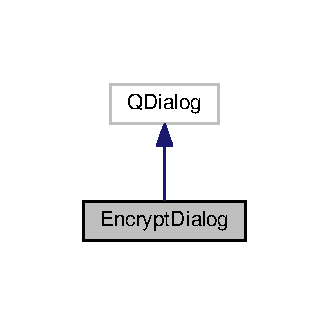
\includegraphics[width=157pt]{class_encrypt_dialog__inherit__graph}
\end{center}
\end{figure}


Collaboration diagram for Encrypt\+Dialog\+:
\nopagebreak
\begin{figure}[H]
\begin{center}
\leavevmode
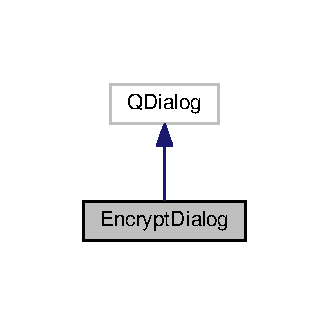
\includegraphics[width=157pt]{class_encrypt_dialog__coll__graph}
\end{center}
\end{figure}
\subsection*{Public Slots}
\begin{DoxyCompactItemize}
\item 
void \mbox{\hyperlink{class_encrypt_dialog_ac9817d3f11f44f4bb8d97a228fbdf8a5}{on\+\_\+file\+Button\+\_\+clicked}} ()
\begin{DoxyCompactList}\small\item\em \mbox{\hyperlink{class_encrypt_dialog_ac9817d3f11f44f4bb8d97a228fbdf8a5}{Encrypt\+Dialog\+::on\+\_\+file\+Button\+\_\+clicked}} Slot to select the image. \end{DoxyCompactList}\item 
void \mbox{\hyperlink{class_encrypt_dialog_a9a998acd37db458eede31f4a9cb16b78}{on\+\_\+button\+Box\+\_\+accepted}} ()
\begin{DoxyCompactList}\small\item\em \mbox{\hyperlink{class_encrypt_dialog_a9a998acd37db458eede31f4a9cb16b78}{Encrypt\+Dialog\+::on\+\_\+button\+Box\+\_\+accepted}} Slot to start the encryption. Successful closing of the app. \end{DoxyCompactList}\item 
void \mbox{\hyperlink{class_encrypt_dialog_a43deb5fd2be501f4d03582a8ed49e9c2}{on\+\_\+button\+Box\+\_\+rejected}} ()
\begin{DoxyCompactList}\small\item\em \mbox{\hyperlink{class_encrypt_dialog_a43deb5fd2be501f4d03582a8ed49e9c2}{Encrypt\+Dialog\+::on\+\_\+button\+Box\+\_\+rejected}} Slot to reject the encryption. \end{DoxyCompactList}\item 
void \mbox{\hyperlink{class_encrypt_dialog_a48c33063066fdbd61e2c87f08a5cfd60}{on\+\_\+horizontal\+Slider\+\_\+value\+Changed}} (int value)
\begin{DoxyCompactList}\small\item\em \mbox{\hyperlink{class_encrypt_dialog_a48c33063066fdbd61e2c87f08a5cfd60}{Encrypt\+Dialog\+::on\+\_\+horizontal\+Slider\+\_\+value\+Changed}} Slot if value of the slider is changed. Key is generated here. \end{DoxyCompactList}\end{DoxyCompactItemize}
\subsection*{Public Member Functions}
\begin{DoxyCompactItemize}
\item 
\mbox{\hyperlink{class_encrypt_dialog_ab57e8b3a0d00c977e81f3b356657524e}{Encrypt\+Dialog}} (Q\+Byte\+Array \+\_\+data, Q\+Widget $\ast$parent=0)
\begin{DoxyCompactList}\small\item\em \mbox{\hyperlink{class_encrypt_dialog_ab57e8b3a0d00c977e81f3b356657524e}{Encrypt\+Dialog\+::\+Encrypt\+Dialog}} Constructor of the class. Input data is saved here and some variables are set here. \end{DoxyCompactList}\item 
\mbox{\hyperlink{class_encrypt_dialog_a466e283080f87ee50f172052e43e38b6}{$\sim$\+Encrypt\+Dialog}} ()
\item 
Q\+Byte\+Array \mbox{\hyperlink{class_encrypt_dialog_a2bff820a3df4ddc36ecb07ed74b7138a}{zip}} ()
\begin{DoxyCompactList}\small\item\em \mbox{\hyperlink{class_encrypt_dialog_a2bff820a3df4ddc36ecb07ed74b7138a}{Encrypt\+Dialog\+::zip}} Zipping algorithm It copresses the data and then compresses it using q\+Compress() \end{DoxyCompactList}\end{DoxyCompactItemize}
\subsection*{Public Attributes}
\begin{DoxyCompactItemize}
\item 
Q\+Byte\+Array \mbox{\hyperlink{class_encrypt_dialog_acf3a8bbce90d99ef17fec093c35b1008}{data}}
\begin{DoxyCompactList}\small\item\em data Input data \end{DoxyCompactList}\item 
bool \mbox{\hyperlink{class_encrypt_dialog_ada4900bcd40894d9c098c65aa4066ac9}{success}}
\begin{DoxyCompactList}\small\item\em success Flag, if image was successfully selected and data was encrypted. \end{DoxyCompactList}\item 
Q\+Byte\+Array \mbox{\hyperlink{class_encrypt_dialog_a3e8998aa39696cbd1242f6420ef18143}{compr\+\_\+data}}
\begin{DoxyCompactList}\small\item\em compr\+\_\+data Compressed data, aka Output data. \end{DoxyCompactList}\item 
Q\+String \mbox{\hyperlink{class_encrypt_dialog_a859b1bc2f032a247632b879bf8663d0b}{input\+File\+Name}}
\begin{DoxyCompactList}\small\item\em input\+File\+Name Filename of the image. \end{DoxyCompactList}\item 
long long int \mbox{\hyperlink{class_encrypt_dialog_a7fff26f838ab50f807744cd2c4bed033}{size}}
\begin{DoxyCompactList}\small\item\em size Size of the image in square pixels \end{DoxyCompactList}\item 
Q\+String \mbox{\hyperlink{class_encrypt_dialog_a1afdef3c665fb0d0fae06d1df8e84951}{key}}
\begin{DoxyCompactList}\small\item\em key Key to be used for encryption in Encryt\+Dialog\+::zip \end{DoxyCompactList}\item 
bool \mbox{\hyperlink{class_encrypt_dialog_a0c821b893cfddd7a6c07bbd270ba49e9}{good\+Percentage}}
\begin{DoxyCompactList}\small\item\em good\+Percentage Flag if area of the used data via encryption is less than 70\% of the area of the image. \end{DoxyCompactList}\item 
int \mbox{\hyperlink{class_encrypt_dialog_a3c9da51b5e9d98d702bcc4ed15405fd5}{val}}
\begin{DoxyCompactList}\small\item\em val Value of the slider \end{DoxyCompactList}\item 
int \mbox{\hyperlink{class_encrypt_dialog_abf638fea37fbdbaba215954e2e239860}{bits\+Used}}
\begin{DoxyCompactList}\small\item\em bits\+Used Bits used per byte of pixel. \end{DoxyCompactList}\item 
Q\+Image \mbox{\hyperlink{class_encrypt_dialog_a739a0df1d28d06b28a3fd16e2bc16c73}{image}}
\begin{DoxyCompactList}\small\item\em image Inputted image \end{DoxyCompactList}\end{DoxyCompactItemize}


\subsection{Detailed Description}
The \mbox{\hyperlink{class_encrypt_dialog}{Encrypt\+Dialog}} class Class to get the image and key to store secret info. 

\begin{DoxyNote}{Note}
Not the most important and well written class. 
\end{DoxyNote}
\begin{DoxySeeAlso}{See also}
\mbox{\hyperlink{class_view_p_c}{View\+PC}} 
\end{DoxySeeAlso}


Definition at line \mbox{\hyperlink{encryptdialog_8h_source_l00021}{21}} of file \mbox{\hyperlink{encryptdialog_8h_source}{encryptdialog.\+h}}.



\subsection{Constructor \& Destructor Documentation}
\mbox{\Hypertarget{class_encrypt_dialog_ab57e8b3a0d00c977e81f3b356657524e}\label{class_encrypt_dialog_ab57e8b3a0d00c977e81f3b356657524e}} 
\index{Encrypt\+Dialog@{Encrypt\+Dialog}!Encrypt\+Dialog@{Encrypt\+Dialog}}
\index{Encrypt\+Dialog@{Encrypt\+Dialog}!Encrypt\+Dialog@{Encrypt\+Dialog}}
\subsubsection{\texorpdfstring{Encrypt\+Dialog()}{EncryptDialog()}}
{\footnotesize\ttfamily Encrypt\+Dialog\+::\+Encrypt\+Dialog (\begin{DoxyParamCaption}\item[{Q\+Byte\+Array}]{\+\_\+data,  }\item[{Q\+Widget $\ast$}]{parent = {\ttfamily 0} }\end{DoxyParamCaption})\hspace{0.3cm}{\ttfamily [explicit]}}



\mbox{\hyperlink{class_encrypt_dialog_ab57e8b3a0d00c977e81f3b356657524e}{Encrypt\+Dialog\+::\+Encrypt\+Dialog}} Constructor of the class. Input data is saved here and some variables are set here. 


\begin{DoxyParams}{Parameters}
{\em \+\_\+data} & Input data. \\
\hline
{\em parent} & Parent (not in use) \\
\hline
\end{DoxyParams}


Definition at line \mbox{\hyperlink{encryptdialog_8cpp_source_l00009}{9}} of file \mbox{\hyperlink{encryptdialog_8cpp_source}{encryptdialog.\+cpp}}.

Here is the call graph for this function\+:
\nopagebreak
\begin{figure}[H]
\begin{center}
\leavevmode
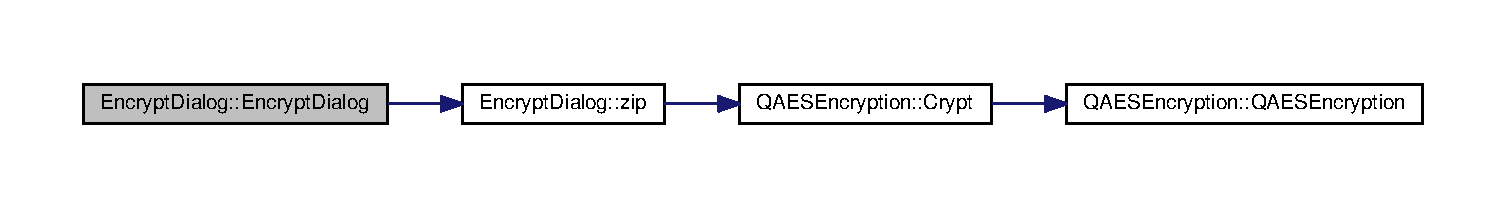
\includegraphics[width=350pt]{class_encrypt_dialog_ab57e8b3a0d00c977e81f3b356657524e_cgraph}
\end{center}
\end{figure}
\mbox{\Hypertarget{class_encrypt_dialog_a466e283080f87ee50f172052e43e38b6}\label{class_encrypt_dialog_a466e283080f87ee50f172052e43e38b6}} 
\index{Encrypt\+Dialog@{Encrypt\+Dialog}!````~Encrypt\+Dialog@{$\sim$\+Encrypt\+Dialog}}
\index{````~Encrypt\+Dialog@{$\sim$\+Encrypt\+Dialog}!Encrypt\+Dialog@{Encrypt\+Dialog}}
\subsubsection{\texorpdfstring{$\sim$\+Encrypt\+Dialog()}{~EncryptDialog()}}
{\footnotesize\ttfamily Encrypt\+Dialog\+::$\sim$\+Encrypt\+Dialog (\begin{DoxyParamCaption}{ }\end{DoxyParamCaption})}



Definition at line \mbox{\hyperlink{encryptdialog_8cpp_source_l00029}{29}} of file \mbox{\hyperlink{encryptdialog_8cpp_source}{encryptdialog.\+cpp}}.



\subsection{Member Function Documentation}
\mbox{\Hypertarget{class_encrypt_dialog_a9a998acd37db458eede31f4a9cb16b78}\label{class_encrypt_dialog_a9a998acd37db458eede31f4a9cb16b78}} 
\index{Encrypt\+Dialog@{Encrypt\+Dialog}!on\+\_\+button\+Box\+\_\+accepted@{on\+\_\+button\+Box\+\_\+accepted}}
\index{on\+\_\+button\+Box\+\_\+accepted@{on\+\_\+button\+Box\+\_\+accepted}!Encrypt\+Dialog@{Encrypt\+Dialog}}
\subsubsection{\texorpdfstring{on\+\_\+button\+Box\+\_\+accepted}{on\_buttonBox\_accepted}}
{\footnotesize\ttfamily void Encrypt\+Dialog\+::on\+\_\+button\+Box\+\_\+accepted (\begin{DoxyParamCaption}{ }\end{DoxyParamCaption})\hspace{0.3cm}{\ttfamily [slot]}}



\mbox{\hyperlink{class_encrypt_dialog_a9a998acd37db458eede31f4a9cb16b78}{Encrypt\+Dialog\+::on\+\_\+button\+Box\+\_\+accepted}} Slot to start the encryption. Successful closing of the app. 



Definition at line \mbox{\hyperlink{encryptdialog_8cpp_source_l00085}{85}} of file \mbox{\hyperlink{encryptdialog_8cpp_source}{encryptdialog.\+cpp}}.

Here is the call graph for this function\+:
\nopagebreak
\begin{figure}[H]
\begin{center}
\leavevmode
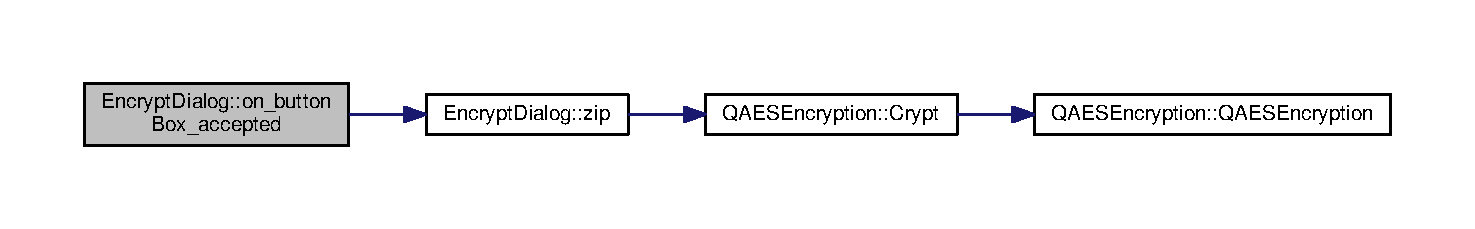
\includegraphics[width=350pt]{class_encrypt_dialog_a9a998acd37db458eede31f4a9cb16b78_cgraph}
\end{center}
\end{figure}
\mbox{\Hypertarget{class_encrypt_dialog_a43deb5fd2be501f4d03582a8ed49e9c2}\label{class_encrypt_dialog_a43deb5fd2be501f4d03582a8ed49e9c2}} 
\index{Encrypt\+Dialog@{Encrypt\+Dialog}!on\+\_\+button\+Box\+\_\+rejected@{on\+\_\+button\+Box\+\_\+rejected}}
\index{on\+\_\+button\+Box\+\_\+rejected@{on\+\_\+button\+Box\+\_\+rejected}!Encrypt\+Dialog@{Encrypt\+Dialog}}
\subsubsection{\texorpdfstring{on\+\_\+button\+Box\+\_\+rejected}{on\_buttonBox\_rejected}}
{\footnotesize\ttfamily void Encrypt\+Dialog\+::on\+\_\+button\+Box\+\_\+rejected (\begin{DoxyParamCaption}{ }\end{DoxyParamCaption})\hspace{0.3cm}{\ttfamily [slot]}}



\mbox{\hyperlink{class_encrypt_dialog_a43deb5fd2be501f4d03582a8ed49e9c2}{Encrypt\+Dialog\+::on\+\_\+button\+Box\+\_\+rejected}} Slot to reject the encryption. 



Definition at line \mbox{\hyperlink{encryptdialog_8cpp_source_l00100}{100}} of file \mbox{\hyperlink{encryptdialog_8cpp_source}{encryptdialog.\+cpp}}.

\mbox{\Hypertarget{class_encrypt_dialog_ac9817d3f11f44f4bb8d97a228fbdf8a5}\label{class_encrypt_dialog_ac9817d3f11f44f4bb8d97a228fbdf8a5}} 
\index{Encrypt\+Dialog@{Encrypt\+Dialog}!on\+\_\+file\+Button\+\_\+clicked@{on\+\_\+file\+Button\+\_\+clicked}}
\index{on\+\_\+file\+Button\+\_\+clicked@{on\+\_\+file\+Button\+\_\+clicked}!Encrypt\+Dialog@{Encrypt\+Dialog}}
\subsubsection{\texorpdfstring{on\+\_\+file\+Button\+\_\+clicked}{on\_fileButton\_clicked}}
{\footnotesize\ttfamily void Encrypt\+Dialog\+::on\+\_\+file\+Button\+\_\+clicked (\begin{DoxyParamCaption}{ }\end{DoxyParamCaption})\hspace{0.3cm}{\ttfamily [slot]}}



\mbox{\hyperlink{class_encrypt_dialog_ac9817d3f11f44f4bb8d97a228fbdf8a5}{Encrypt\+Dialog\+::on\+\_\+file\+Button\+\_\+clicked}} Slot to select the image. 



Definition at line \mbox{\hyperlink{encryptdialog_8cpp_source_l00060}{60}} of file \mbox{\hyperlink{encryptdialog_8cpp_source}{encryptdialog.\+cpp}}.

\mbox{\Hypertarget{class_encrypt_dialog_a48c33063066fdbd61e2c87f08a5cfd60}\label{class_encrypt_dialog_a48c33063066fdbd61e2c87f08a5cfd60}} 
\index{Encrypt\+Dialog@{Encrypt\+Dialog}!on\+\_\+horizontal\+Slider\+\_\+value\+Changed@{on\+\_\+horizontal\+Slider\+\_\+value\+Changed}}
\index{on\+\_\+horizontal\+Slider\+\_\+value\+Changed@{on\+\_\+horizontal\+Slider\+\_\+value\+Changed}!Encrypt\+Dialog@{Encrypt\+Dialog}}
\subsubsection{\texorpdfstring{on\+\_\+horizontal\+Slider\+\_\+value\+Changed}{on\_horizontalSlider\_valueChanged}}
{\footnotesize\ttfamily void Encrypt\+Dialog\+::on\+\_\+horizontal\+Slider\+\_\+value\+Changed (\begin{DoxyParamCaption}\item[{int}]{value }\end{DoxyParamCaption})\hspace{0.3cm}{\ttfamily [slot]}}



\mbox{\hyperlink{class_encrypt_dialog_a48c33063066fdbd61e2c87f08a5cfd60}{Encrypt\+Dialog\+::on\+\_\+horizontal\+Slider\+\_\+value\+Changed}} Slot if value of the slider is changed. Key is generated here. 


\begin{DoxyParams}{Parameters}
{\em value} & Value of the slider. \\
\hline
\end{DoxyParams}


Definition at line \mbox{\hyperlink{encryptdialog_8cpp_source_l00110}{110}} of file \mbox{\hyperlink{encryptdialog_8cpp_source}{encryptdialog.\+cpp}}.

\mbox{\Hypertarget{class_encrypt_dialog_a2bff820a3df4ddc36ecb07ed74b7138a}\label{class_encrypt_dialog_a2bff820a3df4ddc36ecb07ed74b7138a}} 
\index{Encrypt\+Dialog@{Encrypt\+Dialog}!zip@{zip}}
\index{zip@{zip}!Encrypt\+Dialog@{Encrypt\+Dialog}}
\subsubsection{\texorpdfstring{zip()}{zip()}}
{\footnotesize\ttfamily Q\+Byte\+Array Encrypt\+Dialog\+::zip (\begin{DoxyParamCaption}{ }\end{DoxyParamCaption})}



\mbox{\hyperlink{class_encrypt_dialog_a2bff820a3df4ddc36ecb07ed74b7138a}{Encrypt\+Dialog\+::zip}} Zipping algorithm It copresses the data and then compresses it using q\+Compress() 

\begin{DoxyReturn}{Returns}
Returns Compressed data. 
\end{DoxyReturn}
\begin{DoxySeeAlso}{See also}
\mbox{\hyperlink{class_model_p_c_a6da88f166785a49f73b22c169f956fd0}{Model\+P\+C\+::unzip}} 
\end{DoxySeeAlso}


Definition at line \mbox{\hyperlink{encryptdialog_8cpp_source_l00049}{49}} of file \mbox{\hyperlink{encryptdialog_8cpp_source}{encryptdialog.\+cpp}}.

Here is the call graph for this function\+:
\nopagebreak
\begin{figure}[H]
\begin{center}
\leavevmode
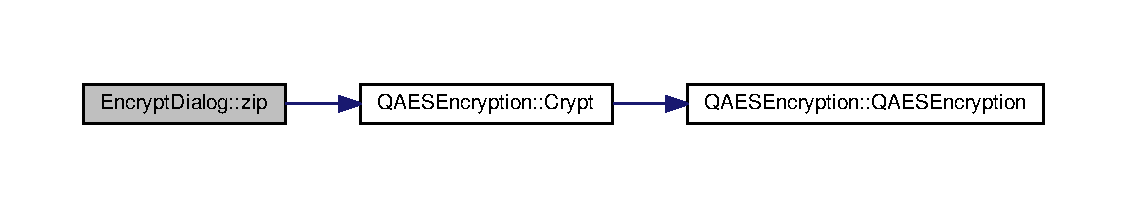
\includegraphics[width=350pt]{class_encrypt_dialog_a2bff820a3df4ddc36ecb07ed74b7138a_cgraph}
\end{center}
\end{figure}
Here is the caller graph for this function\+:
\nopagebreak
\begin{figure}[H]
\begin{center}
\leavevmode
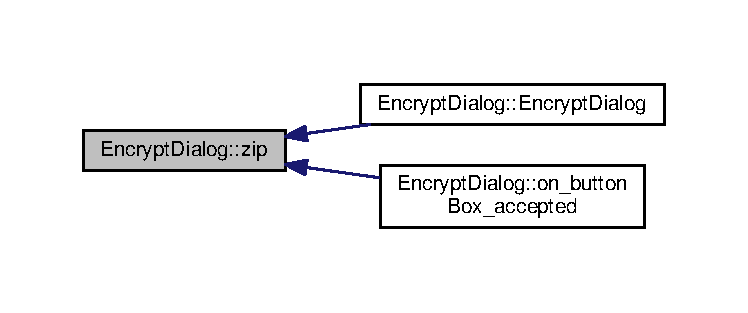
\includegraphics[width=350pt]{class_encrypt_dialog_a2bff820a3df4ddc36ecb07ed74b7138a_icgraph}
\end{center}
\end{figure}


\subsection{Member Data Documentation}
\mbox{\Hypertarget{class_encrypt_dialog_abf638fea37fbdbaba215954e2e239860}\label{class_encrypt_dialog_abf638fea37fbdbaba215954e2e239860}} 
\index{Encrypt\+Dialog@{Encrypt\+Dialog}!bits\+Used@{bits\+Used}}
\index{bits\+Used@{bits\+Used}!Encrypt\+Dialog@{Encrypt\+Dialog}}
\subsubsection{\texorpdfstring{bits\+Used}{bitsUsed}}
{\footnotesize\ttfamily int Encrypt\+Dialog\+::bits\+Used}



bits\+Used Bits used per byte of pixel. 

\begin{DoxySeeAlso}{See also}
\mbox{\hyperlink{class_model_p_c_a1d0091062a0c836b283ec2f67411623b}{Model\+P\+C\+::circuit}} 
\end{DoxySeeAlso}


Definition at line \mbox{\hyperlink{encryptdialog_8h_source_l00075}{75}} of file \mbox{\hyperlink{encryptdialog_8h_source}{encryptdialog.\+h}}.

\mbox{\Hypertarget{class_encrypt_dialog_a3e8998aa39696cbd1242f6420ef18143}\label{class_encrypt_dialog_a3e8998aa39696cbd1242f6420ef18143}} 
\index{Encrypt\+Dialog@{Encrypt\+Dialog}!compr\+\_\+data@{compr\+\_\+data}}
\index{compr\+\_\+data@{compr\+\_\+data}!Encrypt\+Dialog@{Encrypt\+Dialog}}
\subsubsection{\texorpdfstring{compr\+\_\+data}{compr\_data}}
{\footnotesize\ttfamily Q\+Byte\+Array Encrypt\+Dialog\+::compr\+\_\+data}



compr\+\_\+data Compressed data, aka Output data. 



Definition at line \mbox{\hyperlink{encryptdialog_8h_source_l00050}{50}} of file \mbox{\hyperlink{encryptdialog_8h_source}{encryptdialog.\+h}}.

\mbox{\Hypertarget{class_encrypt_dialog_acf3a8bbce90d99ef17fec093c35b1008}\label{class_encrypt_dialog_acf3a8bbce90d99ef17fec093c35b1008}} 
\index{Encrypt\+Dialog@{Encrypt\+Dialog}!data@{data}}
\index{data@{data}!Encrypt\+Dialog@{Encrypt\+Dialog}}
\subsubsection{\texorpdfstring{data}{data}}
{\footnotesize\ttfamily Q\+Byte\+Array Encrypt\+Dialog\+::data}



data Input data 



Definition at line \mbox{\hyperlink{encryptdialog_8h_source_l00042}{42}} of file \mbox{\hyperlink{encryptdialog_8h_source}{encryptdialog.\+h}}.

\mbox{\Hypertarget{class_encrypt_dialog_a0c821b893cfddd7a6c07bbd270ba49e9}\label{class_encrypt_dialog_a0c821b893cfddd7a6c07bbd270ba49e9}} 
\index{Encrypt\+Dialog@{Encrypt\+Dialog}!good\+Percentage@{good\+Percentage}}
\index{good\+Percentage@{good\+Percentage}!Encrypt\+Dialog@{Encrypt\+Dialog}}
\subsubsection{\texorpdfstring{good\+Percentage}{goodPercentage}}
{\footnotesize\ttfamily bool Encrypt\+Dialog\+::good\+Percentage}



good\+Percentage Flag if area of the used data via encryption is less than 70\% of the area of the image. 



Definition at line \mbox{\hyperlink{encryptdialog_8h_source_l00066}{66}} of file \mbox{\hyperlink{encryptdialog_8h_source}{encryptdialog.\+h}}.

\mbox{\Hypertarget{class_encrypt_dialog_a739a0df1d28d06b28a3fd16e2bc16c73}\label{class_encrypt_dialog_a739a0df1d28d06b28a3fd16e2bc16c73}} 
\index{Encrypt\+Dialog@{Encrypt\+Dialog}!image@{image}}
\index{image@{image}!Encrypt\+Dialog@{Encrypt\+Dialog}}
\subsubsection{\texorpdfstring{image}{image}}
{\footnotesize\ttfamily Q\+Image Encrypt\+Dialog\+::image}



image Inputted image 



Definition at line \mbox{\hyperlink{encryptdialog_8h_source_l00079}{79}} of file \mbox{\hyperlink{encryptdialog_8h_source}{encryptdialog.\+h}}.

\mbox{\Hypertarget{class_encrypt_dialog_a859b1bc2f032a247632b879bf8663d0b}\label{class_encrypt_dialog_a859b1bc2f032a247632b879bf8663d0b}} 
\index{Encrypt\+Dialog@{Encrypt\+Dialog}!input\+File\+Name@{input\+File\+Name}}
\index{input\+File\+Name@{input\+File\+Name}!Encrypt\+Dialog@{Encrypt\+Dialog}}
\subsubsection{\texorpdfstring{input\+File\+Name}{inputFileName}}
{\footnotesize\ttfamily Q\+String Encrypt\+Dialog\+::input\+File\+Name}



input\+File\+Name Filename of the image. 



Definition at line \mbox{\hyperlink{encryptdialog_8h_source_l00054}{54}} of file \mbox{\hyperlink{encryptdialog_8h_source}{encryptdialog.\+h}}.

\mbox{\Hypertarget{class_encrypt_dialog_a1afdef3c665fb0d0fae06d1df8e84951}\label{class_encrypt_dialog_a1afdef3c665fb0d0fae06d1df8e84951}} 
\index{Encrypt\+Dialog@{Encrypt\+Dialog}!key@{key}}
\index{key@{key}!Encrypt\+Dialog@{Encrypt\+Dialog}}
\subsubsection{\texorpdfstring{key}{key}}
{\footnotesize\ttfamily Q\+String Encrypt\+Dialog\+::key}



key Key to be used for encryption in Encryt\+Dialog\+::zip 



Definition at line \mbox{\hyperlink{encryptdialog_8h_source_l00062}{62}} of file \mbox{\hyperlink{encryptdialog_8h_source}{encryptdialog.\+h}}.

\mbox{\Hypertarget{class_encrypt_dialog_a7fff26f838ab50f807744cd2c4bed033}\label{class_encrypt_dialog_a7fff26f838ab50f807744cd2c4bed033}} 
\index{Encrypt\+Dialog@{Encrypt\+Dialog}!size@{size}}
\index{size@{size}!Encrypt\+Dialog@{Encrypt\+Dialog}}
\subsubsection{\texorpdfstring{size}{size}}
{\footnotesize\ttfamily long long int Encrypt\+Dialog\+::size}



size Size of the image in square pixels 



Definition at line \mbox{\hyperlink{encryptdialog_8h_source_l00058}{58}} of file \mbox{\hyperlink{encryptdialog_8h_source}{encryptdialog.\+h}}.

\mbox{\Hypertarget{class_encrypt_dialog_ada4900bcd40894d9c098c65aa4066ac9}\label{class_encrypt_dialog_ada4900bcd40894d9c098c65aa4066ac9}} 
\index{Encrypt\+Dialog@{Encrypt\+Dialog}!success@{success}}
\index{success@{success}!Encrypt\+Dialog@{Encrypt\+Dialog}}
\subsubsection{\texorpdfstring{success}{success}}
{\footnotesize\ttfamily bool Encrypt\+Dialog\+::success}



success Flag, if image was successfully selected and data was encrypted. 



Definition at line \mbox{\hyperlink{encryptdialog_8h_source_l00046}{46}} of file \mbox{\hyperlink{encryptdialog_8h_source}{encryptdialog.\+h}}.

\mbox{\Hypertarget{class_encrypt_dialog_a3c9da51b5e9d98d702bcc4ed15405fd5}\label{class_encrypt_dialog_a3c9da51b5e9d98d702bcc4ed15405fd5}} 
\index{Encrypt\+Dialog@{Encrypt\+Dialog}!val@{val}}
\index{val@{val}!Encrypt\+Dialog@{Encrypt\+Dialog}}
\subsubsection{\texorpdfstring{val}{val}}
{\footnotesize\ttfamily int Encrypt\+Dialog\+::val}



val Value of the slider 



Definition at line \mbox{\hyperlink{encryptdialog_8h_source_l00070}{70}} of file \mbox{\hyperlink{encryptdialog_8h_source}{encryptdialog.\+h}}.



The documentation for this class was generated from the following files\+:\begin{DoxyCompactItemize}
\item 
C\+:/\+Users/salex/\+Documents/\+Git\+Hub/\+Picture\+Crypt/src/\mbox{\hyperlink{encryptdialog_8h}{encryptdialog.\+h}}\item 
C\+:/\+Users/salex/\+Documents/\+Git\+Hub/\+Picture\+Crypt/src/\mbox{\hyperlink{encryptdialog_8cpp}{encryptdialog.\+cpp}}\end{DoxyCompactItemize}

\hypertarget{class_model_p_c}{}\section{Model\+PC Class Reference}
\label{class_model_p_c}\index{Model\+PC@{Model\+PC}}


The \hyperlink{class_model_p_c}{Model\+PC} class Model Layer of the app. Main class that does the work of Picture\+Crypt logic Controled by \hyperlink{class_controller_p_c}{Controller\+PC}.  




{\ttfamily \#include $<$modelpc.\+h$>$}



Inheritance diagram for Model\+PC\+:
\nopagebreak
\begin{figure}[H]
\begin{center}
\leavevmode
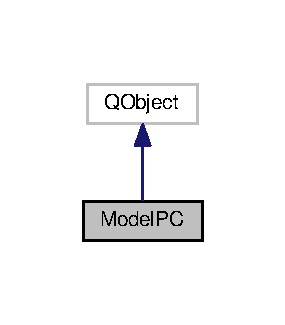
\includegraphics[width=137pt]{class_model_p_c__inherit__graph}
\end{center}
\end{figure}


Collaboration diagram for Model\+PC\+:
\nopagebreak
\begin{figure}[H]
\begin{center}
\leavevmode
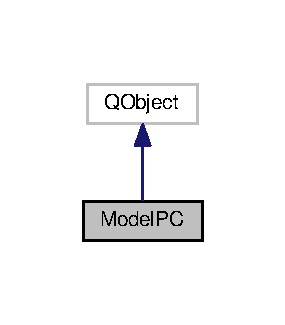
\includegraphics[width=137pt]{class_model_p_c__coll__graph}
\end{center}
\end{figure}
\subsection*{Public Types}
\begin{DoxyCompactItemize}
\item 
enum \hyperlink{class_model_p_c_a296dd7afe3e1c49b3da25fd644fe4ceb}{Crypt\+Mode} \{ \hyperlink{class_model_p_c_a296dd7afe3e1c49b3da25fd644fe4ceba287198790ac9799acd03c99d63a6faea}{Not\+Defined}, 
\hyperlink{class_model_p_c_a296dd7afe3e1c49b3da25fd644fe4ceba7612e38de7178170655a56ddcf96e12c}{v1\+\_\+3}, 
\hyperlink{class_model_p_c_a296dd7afe3e1c49b3da25fd644fe4ceba43138df6b33a6b2bf608768907f95abc}{v1\+\_\+4}, 
\hyperlink{class_model_p_c_a296dd7afe3e1c49b3da25fd644fe4ceba90ca32d3ccbb6be224cdfc33f7096eea}{jphs\+\_\+mode}
 \}
\end{DoxyCompactItemize}
\subsection*{Public Slots}
\begin{DoxyCompactItemize}
\item 
Q\+Image $\ast$ \hyperlink{class_model_p_c_a6f191f62d4635d0d3555fcc0be298794}{encrypt} (Q\+Byte\+Array data, Q\+Image $\ast$image, int \+\_\+mode, Q\+String key=\char`\"{}\char`\"{}, int \+\_\+bits\+Used=8, Q\+String $\ast$\+\_\+error=nullptr)
\begin{DoxyCompactList}\small\item\em \hyperlink{class_model_p_c_a6f191f62d4635d0d3555fcc0be298794}{Model\+P\+C\+::encrypt} Slot to zip and inject data and provide it with some extra stuff After completion start standard \hyperlink{class_model_p_c_aada6a04d81ada8f2b4ba18108c8d6f10}{Model\+P\+C\+::inject} Isn\textquotesingle{}t used in Picture\+Crypt, but used can be used in other -\/ custom projects. \end{DoxyCompactList}\item 
Q\+Image $\ast$ \hyperlink{class_model_p_c_aada6a04d81ada8f2b4ba18108c8d6f10}{inject} (Q\+Byte\+Array encr\+\_\+data, Q\+Image $\ast$image, int \+\_\+mode, int \+\_\+bits\+Used=8, Q\+String $\ast$\+\_\+error=nullptr)
\begin{DoxyCompactList}\small\item\em \hyperlink{class_model_p_c_aada6a04d81ada8f2b4ba18108c8d6f10}{Model\+P\+C\+::inject} Slot to be called when encrypt mode in \hyperlink{class_view_p_c}{View\+PC} is selected and started. \end{DoxyCompactList}\item 
Q\+Byte\+Array \hyperlink{class_model_p_c_a5995215a34a1e1f504035715a8013809}{decrypt} (Q\+Image $\ast$image, Q\+String key, int \+\_\+mode=0, Q\+String $\ast$\+\_\+error=nullptr)
\begin{DoxyCompactList}\small\item\em \hyperlink{class_model_p_c_a5995215a34a1e1f504035715a8013809}{Model\+P\+C\+::decrypt} Slot to be called when decrypt mode in \hyperlink{class_view_p_c}{View\+PC} is selected and started. \end{DoxyCompactList}\item 
void \hyperlink{class_model_p_c_a47464b59b7e37fcee25e55475708aabd}{fail} (Q\+String message)
\begin{DoxyCompactList}\small\item\em \hyperlink{class_model_p_c_a47464b59b7e37fcee25e55475708aabd}{Model\+P\+C\+::fail} Slot to stop execution of cryption. \end{DoxyCompactList}\item 
void \hyperlink{class_model_p_c_a9079a101d83672aa48fd2dbac797de40}{alert} (Q\+String message, bool is\+Warning=false)
\begin{DoxyCompactList}\small\item\em \hyperlink{class_model_p_c_a9079a101d83672aa48fd2dbac797de40}{Model\+P\+C\+::alert} Function emits signal \hyperlink{class_model_p_c_af0217a7ca5671e26090dc50a5dccdaf5}{Model\+P\+C\+::alert\+View} and calls \hyperlink{class_view_p_c_a7c467169467789561078abc9d4fe57bd}{View\+P\+C\+::alert}. \end{DoxyCompactList}\end{DoxyCompactItemize}
\subsection*{Signals}
\begin{DoxyCompactItemize}
\item 
void \hyperlink{class_model_p_c_af0217a7ca5671e26090dc50a5dccdaf5}{alert\+View} (Q\+String message\+Code, bool is\+Warning)
\begin{DoxyCompactList}\small\item\em alert\+View Signal to be called to create Message\+Box. \end{DoxyCompactList}\item 
void \hyperlink{class_model_p_c_a0855107fb0ccc247cd9e893fae9bb08a}{save\+Data} (Q\+Byte\+Array data)
\begin{DoxyCompactList}\small\item\em save\+Data Signal to be called to save data from \hyperlink{class_model_p_c_a5995215a34a1e1f504035715a8013809}{Model\+P\+C\+::decrypt}. \end{DoxyCompactList}\item 
void \hyperlink{class_model_p_c_a41f5e2e8022679046e4d3fa1109025fa}{save\+Image} (Q\+Image $\ast$image)
\begin{DoxyCompactList}\small\item\em save\+Image Signal to be called to save image from \hyperlink{class_model_p_c_a6f191f62d4635d0d3555fcc0be298794}{Model\+P\+C\+::encrypt}. \end{DoxyCompactList}\item 
void \hyperlink{class_model_p_c_afdcd80f0ed5062e145a71f09b0897547}{set\+Progress} (int val)
\begin{DoxyCompactList}\small\item\em set\+Progress Signal to be called to set progress of Progress\+Dialog. \end{DoxyCompactList}\end{DoxyCompactItemize}
\subsection*{Public Member Functions}
\begin{DoxyCompactItemize}
\item 
\hyperlink{class_model_p_c_ae12ebe65ec973c02a0de4850a7c1e31c}{Model\+PC} ()
\begin{DoxyCompactList}\small\item\em \hyperlink{class_model_p_c_ae12ebe65ec973c02a0de4850a7c1e31c}{Model\+P\+C\+::\+Model\+PC} Constructor Unit tests are run here. \end{DoxyCompactList}\item 
Q\+Byte\+Array \hyperlink{class_model_p_c_a6da88f166785a49f73b22c169f956fd0}{unzip} (Q\+Byte\+Array data, Q\+Byte\+Array key)
\begin{DoxyCompactList}\small\item\em \hyperlink{class_model_p_c_a6da88f166785a49f73b22c169f956fd0}{Model\+P\+C\+::unzip} Unzip data from \hyperlink{class_model_p_c_a5995215a34a1e1f504035715a8013809}{Model\+P\+C\+::decrypt}. Just mirrored \hyperlink{class_encrypt_dialog_a2bff820a3df4ddc36ecb07ed74b7138a}{Encrypt\+Dialog\+::zip}. \end{DoxyCompactList}\end{DoxyCompactItemize}
\subsection*{Static Public Member Functions}
\begin{DoxyCompactItemize}
\item 
static Q\+Image $\ast$ \hyperlink{class_model_p_c_a271cf9285e32df58ffbfc918e6482bbd}{Encrypt} (Q\+Byte\+Array data, Q\+Image $\ast$image, int \+\_\+mode, Q\+String key=\char`\"{}\char`\"{}, int \+\_\+bits\+Used=8, Q\+String $\ast$\+\_\+error=nullptr)
\item 
static Q\+Image $\ast$ \hyperlink{class_model_p_c_ac17e68e6aab134621b0d151d74acdc82}{Inject} (Q\+Byte\+Array encr\+\_\+data, Q\+Image $\ast$image, int \+\_\+mode, int \+\_\+bits\+Used=8, Q\+String $\ast$\+\_\+error=nullptr)
\item 
static Q\+Byte\+Array \hyperlink{class_model_p_c_a902abaea4f07995b48c0f2fea6eceb7c}{Decrypt} (Q\+Image $\ast$image, Q\+String key, int \+\_\+mode=0, Q\+String $\ast$\+\_\+error=nullptr)
\end{DoxyCompactItemize}
\subsection*{Public Attributes}
\begin{DoxyCompactItemize}
\item 
bool \hyperlink{class_model_p_c_a945ffbbc44a832b953c191debd448f4c}{success}
\begin{DoxyCompactList}\small\item\em success Flag that true by default, but in case of error or cancelling of Progress\+Dialog it turns to false, which stops execution of \hyperlink{class_model_p_c_a1d0091062a0c836b283ec2f67411623b}{Model\+P\+C\+::circuit} \end{DoxyCompactList}\item 
long \hyperlink{class_model_p_c_a5af48ab89e19be42a94c34ba00249401}{version}
\begin{DoxyCompactList}\small\item\em version Version of the class \end{DoxyCompactList}\item 
Q\+String \hyperlink{class_model_p_c_a5f426725ccf7eefd3c77ea8c720264c9}{version\+String}
\begin{DoxyCompactList}\small\item\em version\+String Version as string \end{DoxyCompactList}\item 
Q\+String \hyperlink{class_model_p_c_abd038306f14f22fb885a1697c96d6335}{default\+J\+P\+H\+S\+Dir}
\begin{DoxyCompactList}\small\item\em default\+J\+P\+H\+S\+Dir Default J\+P\+HS directory \end{DoxyCompactList}\end{DoxyCompactItemize}
\subsection*{Protected Member Functions}
\begin{DoxyCompactItemize}
\item 
void \hyperlink{class_model_p_c_a1d0091062a0c836b283ec2f67411623b}{circuit} (Q\+Image $\ast$image, Q\+Byte\+Array $\ast$data, long long int count\+Bytes)
\begin{DoxyCompactList}\small\item\em \hyperlink{class_model_p_c_a1d0091062a0c836b283ec2f67411623b}{Model\+P\+C\+::circuit} The brain of the app. Via special circuit stores data in image. \end{DoxyCompactList}\item 
void \hyperlink{class_model_p_c_a8bee0255c09449868c7e6097afaaf0cd}{jphs} (Q\+Image $\ast$image, Q\+Byte\+Array $\ast$data)
\begin{DoxyCompactList}\small\item\em \hyperlink{class_model_p_c_a8bee0255c09449868c7e6097afaaf0cd}{Model\+P\+C\+::jphs} J\+P\+HS function to use jphide and jpseek (currently under development) \end{DoxyCompactList}\item 
void \hyperlink{class_model_p_c_a1171f9fe1550133dc9053a46b4e5bcfd}{process\+Pixel} (Q\+Point pos, Q\+Vector$<$ Q\+Point $>$ $\ast$were, bool is\+Encrypt)
\begin{DoxyCompactList}\small\item\em \hyperlink{class_model_p_c_a1171f9fe1550133dc9053a46b4e5bcfd}{Model\+P\+C\+::process\+Pixel} Processes every pixel. Reads its contains or writes data. \end{DoxyCompactList}\item 
void \hyperlink{class_model_p_c_a4daefc3fb87a1f19172b9b20c987eb12}{encryptv1\+\_\+4} (Q\+Image $\ast$image, Q\+Byte\+Array data, Q\+String key)
\begin{DoxyCompactList}\small\item\em \hyperlink{class_model_p_c_a4daefc3fb87a1f19172b9b20c987eb12}{Model\+P\+C\+::encryptv1\+\_\+4} Encrypts and injects data to image used in v1.\+4+. \end{DoxyCompactList}\item 
Q\+Byte\+Array \hyperlink{class_model_p_c_a4fe70ebbedfaf31d45a35f82d0f06caa}{decryptv1\+\_\+3} (Q\+Image $\ast$image, Q\+String key)
\begin{DoxyCompactList}\small\item\em \hyperlink{class_model_p_c_a4fe70ebbedfaf31d45a35f82d0f06caa}{Model\+P\+C\+::decryptv1\+\_\+3} Decrytps data from image in v1.\+3. \end{DoxyCompactList}\item 
Q\+Byte\+Array \hyperlink{class_model_p_c_a7a1f7d491e1bde16936190b9e90896b0}{decryptv1\+\_\+4} (Q\+Image $\ast$image, Q\+String key)
\begin{DoxyCompactList}\small\item\em \hyperlink{class_model_p_c_a7a1f7d491e1bde16936190b9e90896b0}{Model\+P\+C\+::decryptv1\+\_\+4} Decrypts data from image in v1.\+4+. \end{DoxyCompactList}\item 
void \hyperlink{class_model_p_c_a5cdb4d1d61ff62ee9d45b496a7dbf1fb}{proccess\+Pixelsv1\+\_\+4} (Q\+Image $\ast$image, Q\+Byte\+Array $\ast$data, Q\+Byte\+Array key, bool is\+Encrypt, Q\+Vector$<$ Q\+Pair$<$ Q\+Point, Q\+Pair$<$ int, int $>$ $>$ $>$ $\ast$were, long long size=-\/1)
\begin{DoxyCompactList}\small\item\em \hyperlink{class_model_p_c_a5cdb4d1d61ff62ee9d45b496a7dbf1fb}{Model\+P\+C\+::proccess\+Pixelsv1\+\_\+4} Hides (or retrieves) data to/from pixels. \end{DoxyCompactList}\item 
Q\+Byte\+Array \hyperlink{class_model_p_c_afebbbfa4b07deba4f68fc6dfb50f353f}{zip} (Q\+Byte\+Array data, Q\+Byte\+Array key)
\begin{DoxyCompactList}\small\item\em \hyperlink{class_model_p_c_afebbbfa4b07deba4f68fc6dfb50f353f}{Model\+P\+C\+::zip} Zip function, copy of \hyperlink{class_encrypt_dialog_a2bff820a3df4ddc36ecb07ed74b7138a}{Encrypt\+Dialog\+::zip} Used for \hyperlink{class_model_p_c}{Model\+PC} in custom projects, other than Picture\+Crypt. \end{DoxyCompactList}\end{DoxyCompactItemize}
\subsection*{Protected Attributes}
\begin{DoxyCompactItemize}
\item 
Q\+String $\ast$ \hyperlink{class_model_p_c_a4e5a9c0ca1f06fe5bc478b6bf248c37c}{error}
\begin{DoxyCompactList}\small\item\em error Current error \end{DoxyCompactList}\end{DoxyCompactItemize}


\subsection{Detailed Description}
The \hyperlink{class_model_p_c}{Model\+PC} class Model Layer of the app. Main class that does the work of Picture\+Crypt logic Controled by \hyperlink{class_controller_p_c}{Controller\+PC}. 

\begin{DoxySeeAlso}{See also}
\hyperlink{class_view_p_c}{View\+PC}, \hyperlink{class_controller_p_c}{Controller\+PC} 
\end{DoxySeeAlso}
\begin{DoxyAuthor}{Author}
Alex Kovrigin (waleko) 
\end{DoxyAuthor}


Definition at line \hyperlink{modelpc_8h_source_l00033}{33} of file \hyperlink{modelpc_8h_source}{modelpc.\+h}.



\subsection{Member Enumeration Documentation}
\index{Model\+PC@{Model\+PC}!Crypt\+Mode@{Crypt\+Mode}}
\index{Crypt\+Mode@{Crypt\+Mode}!Model\+PC@{Model\+PC}}
\subsubsection[{\texorpdfstring{Crypt\+Mode}{CryptMode}}]{\setlength{\rightskip}{0pt plus 5cm}enum {\bf Model\+P\+C\+::\+Crypt\+Mode}}\hypertarget{class_model_p_c_a296dd7afe3e1c49b3da25fd644fe4ceb}{}\label{class_model_p_c_a296dd7afe3e1c49b3da25fd644fe4ceb}
\begin{Desc}
\item[Enumerator]\par
\begin{description}
\index{Not\+Defined@{Not\+Defined}!Model\+PC@{Model\+PC}}\index{Model\+PC@{Model\+PC}!Not\+Defined@{Not\+Defined}}\item[{\em 
Not\+Defined\hypertarget{class_model_p_c_a296dd7afe3e1c49b3da25fd644fe4ceba287198790ac9799acd03c99d63a6faea}{}\label{class_model_p_c_a296dd7afe3e1c49b3da25fd644fe4ceba287198790ac9799acd03c99d63a6faea}
}]\index{v1\+\_\+3@{v1\+\_\+3}!Model\+PC@{Model\+PC}}\index{Model\+PC@{Model\+PC}!v1\+\_\+3@{v1\+\_\+3}}\item[{\em 
v1\+\_\+3\hypertarget{class_model_p_c_a296dd7afe3e1c49b3da25fd644fe4ceba7612e38de7178170655a56ddcf96e12c}{}\label{class_model_p_c_a296dd7afe3e1c49b3da25fd644fe4ceba7612e38de7178170655a56ddcf96e12c}
}]\index{v1\+\_\+4@{v1\+\_\+4}!Model\+PC@{Model\+PC}}\index{Model\+PC@{Model\+PC}!v1\+\_\+4@{v1\+\_\+4}}\item[{\em 
v1\+\_\+4\hypertarget{class_model_p_c_a296dd7afe3e1c49b3da25fd644fe4ceba43138df6b33a6b2bf608768907f95abc}{}\label{class_model_p_c_a296dd7afe3e1c49b3da25fd644fe4ceba43138df6b33a6b2bf608768907f95abc}
}]\index{jphs\+\_\+mode@{jphs\+\_\+mode}!Model\+PC@{Model\+PC}}\index{Model\+PC@{Model\+PC}!jphs\+\_\+mode@{jphs\+\_\+mode}}\item[{\em 
jphs\+\_\+mode\hypertarget{class_model_p_c_a296dd7afe3e1c49b3da25fd644fe4ceba90ca32d3ccbb6be224cdfc33f7096eea}{}\label{class_model_p_c_a296dd7afe3e1c49b3da25fd644fe4ceba90ca32d3ccbb6be224cdfc33f7096eea}
}]\end{description}
\end{Desc}


Definition at line \hyperlink{modelpc_8h_source_l00038}{38} of file \hyperlink{modelpc_8h_source}{modelpc.\+h}.



\subsection{Constructor \& Destructor Documentation}
\index{Model\+PC@{Model\+PC}!Model\+PC@{Model\+PC}}
\index{Model\+PC@{Model\+PC}!Model\+PC@{Model\+PC}}
\subsubsection[{\texorpdfstring{Model\+P\+C()}{ModelPC()}}]{\setlength{\rightskip}{0pt plus 5cm}Model\+P\+C\+::\+Model\+PC (
\begin{DoxyParamCaption}
{}
\end{DoxyParamCaption}
)}\hypertarget{class_model_p_c_ae12ebe65ec973c02a0de4850a7c1e31c}{}\label{class_model_p_c_ae12ebe65ec973c02a0de4850a7c1e31c}


\hyperlink{class_model_p_c_ae12ebe65ec973c02a0de4850a7c1e31c}{Model\+P\+C\+::\+Model\+PC} Constructor Unit tests are run here. 

\begin{DoxySeeAlso}{See also}
\hyperlink{class_controller_p_c}{Controller\+PC}, \hyperlink{class_view_p_c}{View\+PC} 
\end{DoxySeeAlso}


Definition at line \hyperlink{modelpc_8cpp_source_l00009}{9} of file \hyperlink{modelpc_8cpp_source}{modelpc.\+cpp}.



Here is the caller graph for this function\+:
\nopagebreak
\begin{figure}[H]
\begin{center}
\leavevmode
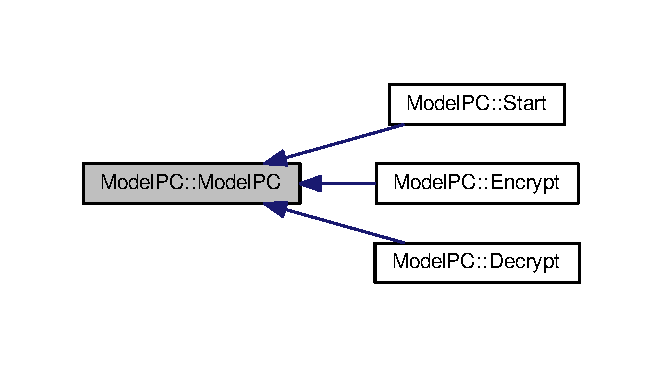
\includegraphics[width=318pt]{class_model_p_c_ae12ebe65ec973c02a0de4850a7c1e31c_icgraph}
\end{center}
\end{figure}




\subsection{Member Function Documentation}
\index{Model\+PC@{Model\+PC}!alert@{alert}}
\index{alert@{alert}!Model\+PC@{Model\+PC}}
\subsubsection[{\texorpdfstring{alert}{alert}}]{\setlength{\rightskip}{0pt plus 5cm}void Model\+P\+C\+::alert (
\begin{DoxyParamCaption}
\item[{Q\+String}]{message, }
\item[{bool}]{is\+Warning = {\ttfamily false}}
\end{DoxyParamCaption}
)\hspace{0.3cm}{\ttfamily [slot]}}\hypertarget{class_model_p_c_a9079a101d83672aa48fd2dbac797de40}{}\label{class_model_p_c_a9079a101d83672aa48fd2dbac797de40}


\hyperlink{class_model_p_c_a9079a101d83672aa48fd2dbac797de40}{Model\+P\+C\+::alert} Function emits signal \hyperlink{class_model_p_c_af0217a7ca5671e26090dc50a5dccdaf5}{Model\+P\+C\+::alert\+View} and calls \hyperlink{class_view_p_c_a7c467169467789561078abc9d4fe57bd}{View\+P\+C\+::alert}. 


\begin{DoxyParams}{Parameters}
{\em message} & Message to be transmitted. \\
\hline
{\em is\+Warning} & Flag if message is critical. \\
\hline
\end{DoxyParams}
\begin{DoxySeeAlso}{See also}
\hyperlink{class_view_p_c_a7c467169467789561078abc9d4fe57bd}{View\+P\+C\+::alert} 
\end{DoxySeeAlso}


Definition at line \hyperlink{modelpc_8cpp_source_l00937}{937} of file \hyperlink{modelpc_8cpp_source}{modelpc.\+cpp}.



Here is the caller graph for this function\+:
\nopagebreak
\begin{figure}[H]
\begin{center}
\leavevmode
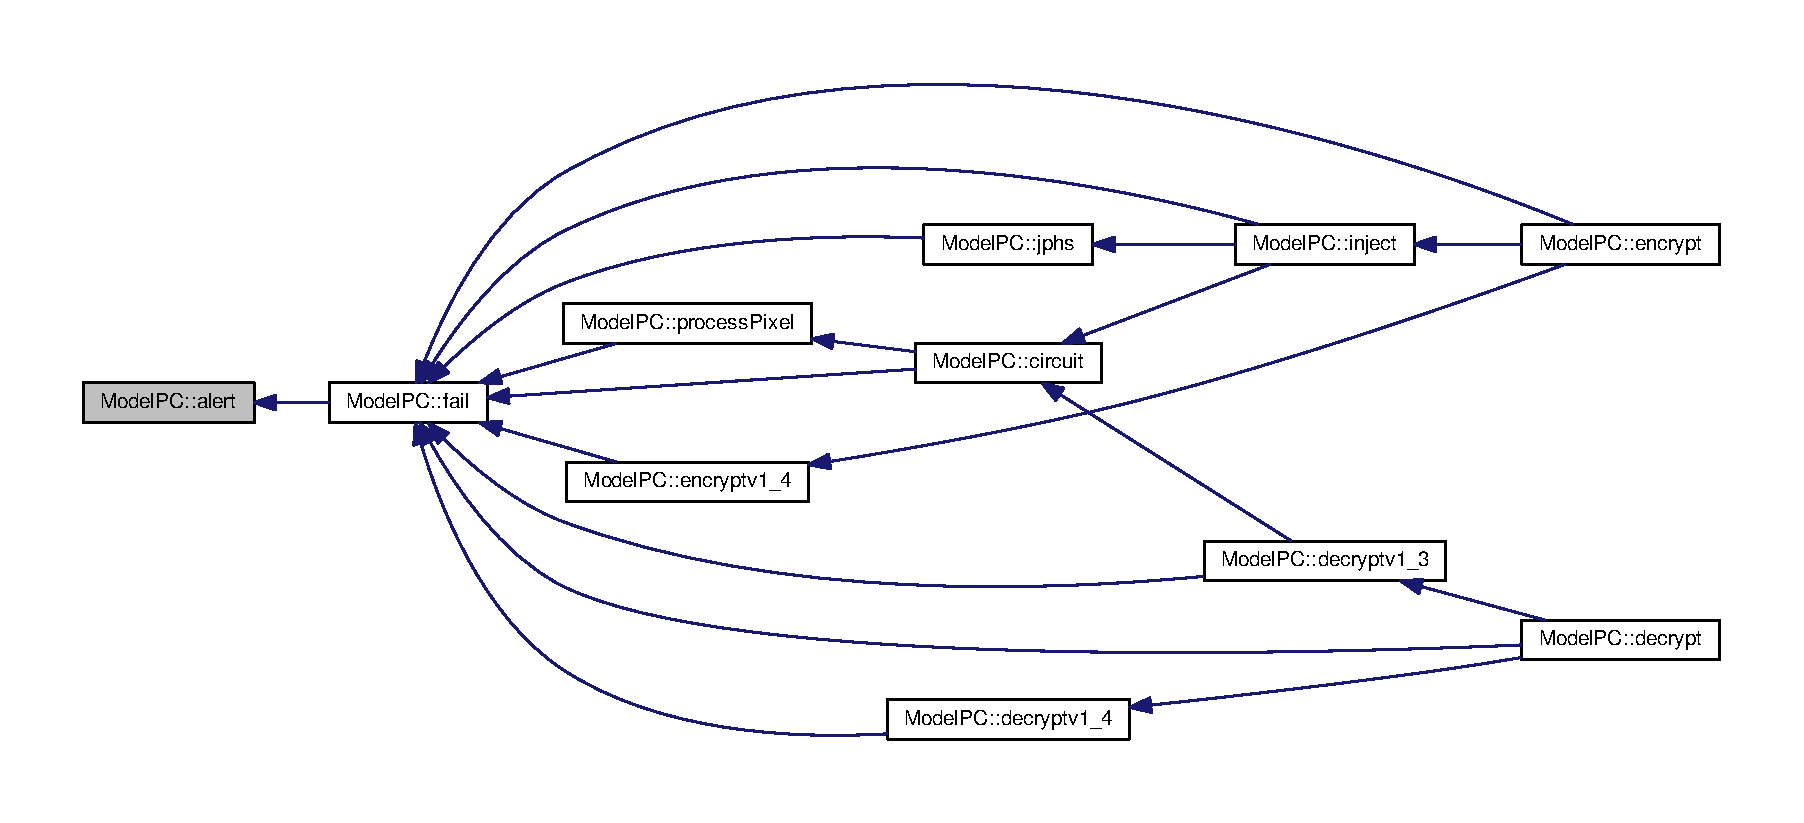
\includegraphics[width=350pt]{class_model_p_c_a9079a101d83672aa48fd2dbac797de40_icgraph}
\end{center}
\end{figure}


\index{Model\+PC@{Model\+PC}!alert\+View@{alert\+View}}
\index{alert\+View@{alert\+View}!Model\+PC@{Model\+PC}}
\subsubsection[{\texorpdfstring{alert\+View}{alertView}}]{\setlength{\rightskip}{0pt plus 5cm}void Model\+P\+C\+::alert\+View (
\begin{DoxyParamCaption}
\item[{Q\+String}]{message\+Code, }
\item[{bool}]{is\+Warning}
\end{DoxyParamCaption}
)\hspace{0.3cm}{\ttfamily [signal]}}\hypertarget{class_model_p_c_af0217a7ca5671e26090dc50a5dccdaf5}{}\label{class_model_p_c_af0217a7ca5671e26090dc50a5dccdaf5}


alert\+View Signal to be called to create Message\+Box. 


\begin{DoxyParams}{Parameters}
{\em message\+Code} & Message Code to be shown. \\
\hline
{\em is\+Warning} & Flag if message is critical. \\
\hline
\end{DoxyParams}
\begin{DoxySeeAlso}{See also}
\hyperlink{class_model_p_c_a9079a101d83672aa48fd2dbac797de40}{Model\+P\+C\+::alert}, \hyperlink{class_view_p_c_a7c467169467789561078abc9d4fe57bd}{View\+P\+C\+::alert} 
\end{DoxySeeAlso}


Here is the caller graph for this function\+:
\nopagebreak
\begin{figure}[H]
\begin{center}
\leavevmode
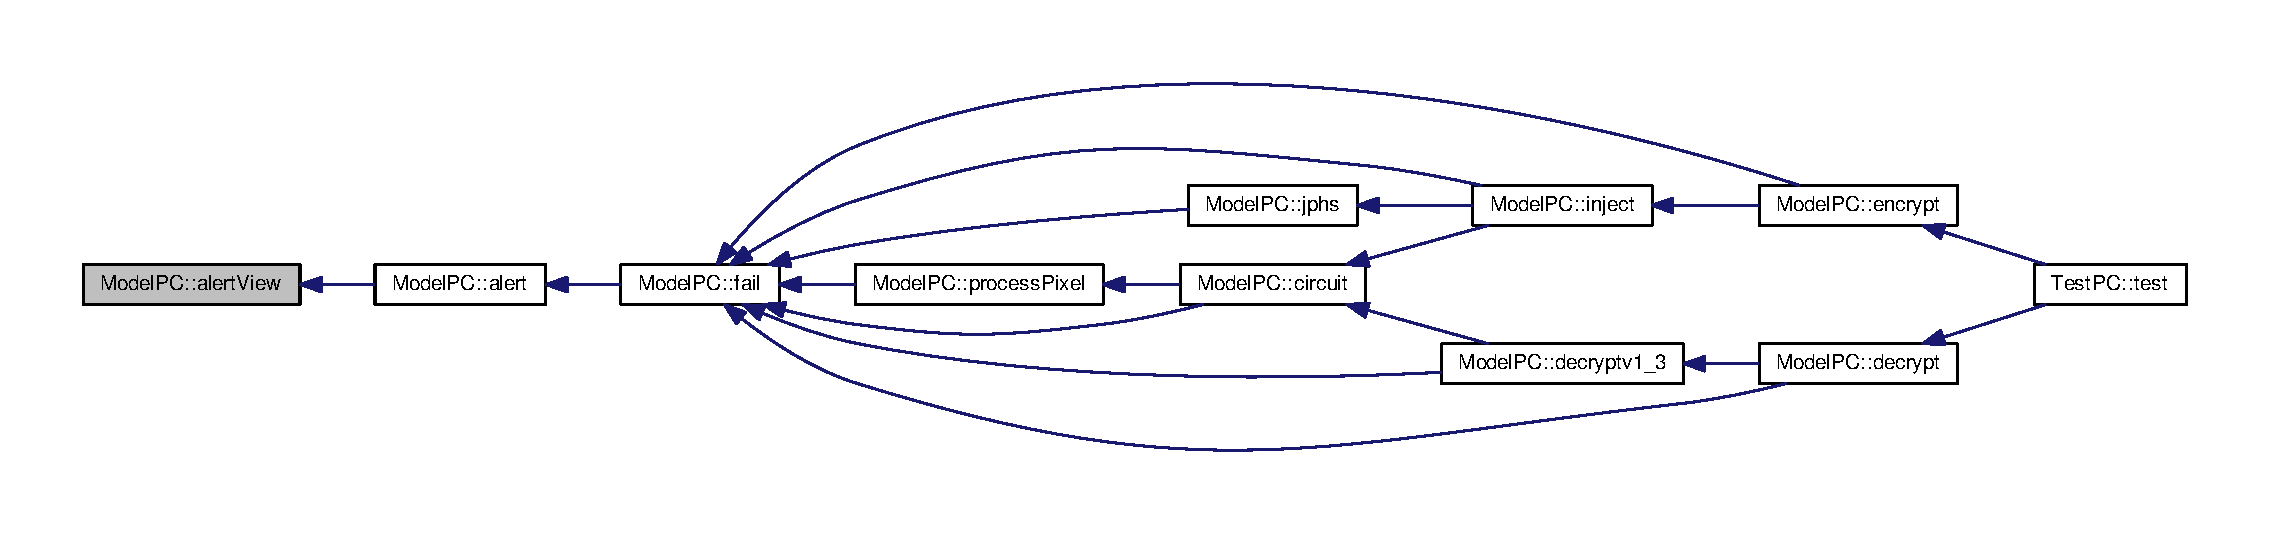
\includegraphics[width=350pt]{class_model_p_c_af0217a7ca5671e26090dc50a5dccdaf5_icgraph}
\end{center}
\end{figure}


\index{Model\+PC@{Model\+PC}!circuit@{circuit}}
\index{circuit@{circuit}!Model\+PC@{Model\+PC}}
\subsubsection[{\texorpdfstring{circuit(\+Q\+Image $\ast$image, Q\+Byte\+Array $\ast$data, long long int count\+Bytes)}{circuit(QImage *image, QByteArray *data, long long int countBytes)}}]{\setlength{\rightskip}{0pt plus 5cm}void Model\+P\+C\+::circuit (
\begin{DoxyParamCaption}
\item[{Q\+Image $\ast$}]{image, }
\item[{Q\+Byte\+Array $\ast$}]{data, }
\item[{long long int}]{count\+Bytes}
\end{DoxyParamCaption}
)\hspace{0.3cm}{\ttfamily [protected]}}\hypertarget{class_model_p_c_a1d0091062a0c836b283ec2f67411623b}{}\label{class_model_p_c_a1d0091062a0c836b283ec2f67411623b}


\hyperlink{class_model_p_c_a1d0091062a0c836b283ec2f67411623b}{Model\+P\+C\+::circuit} The brain of the app. Via special circuit stores data in image. 

The circuit itself can be found in documentation or in commentaries in source. 
\begin{DoxyParams}{Parameters}
{\em image} & Image to be processed. \\
\hline
{\em data} & Data to be processed. \\
\hline
{\em count\+Bytes} & Number of bytes to be read or written. \\
\hline
\end{DoxyParams}
\begin{DoxySeeAlso}{See also}
\hyperlink{class_model_p_c_a1171f9fe1550133dc9053a46b4e5bcfd}{Model\+P\+C\+::process\+Pixel} 
\end{DoxySeeAlso}


Definition at line \hyperlink{modelpc_8cpp_source_l00356}{356} of file \hyperlink{modelpc_8cpp_source}{modelpc.\+cpp}.



Here is the call graph for this function\+:
\nopagebreak
\begin{figure}[H]
\begin{center}
\leavevmode
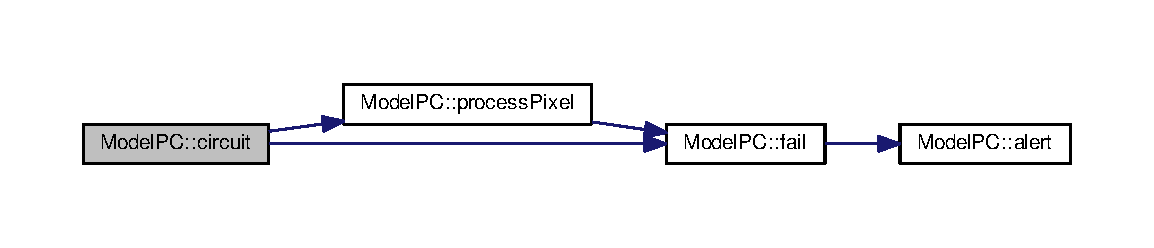
\includegraphics[width=350pt]{class_model_p_c_a1d0091062a0c836b283ec2f67411623b_cgraph}
\end{center}
\end{figure}




Here is the caller graph for this function\+:
\nopagebreak
\begin{figure}[H]
\begin{center}
\leavevmode
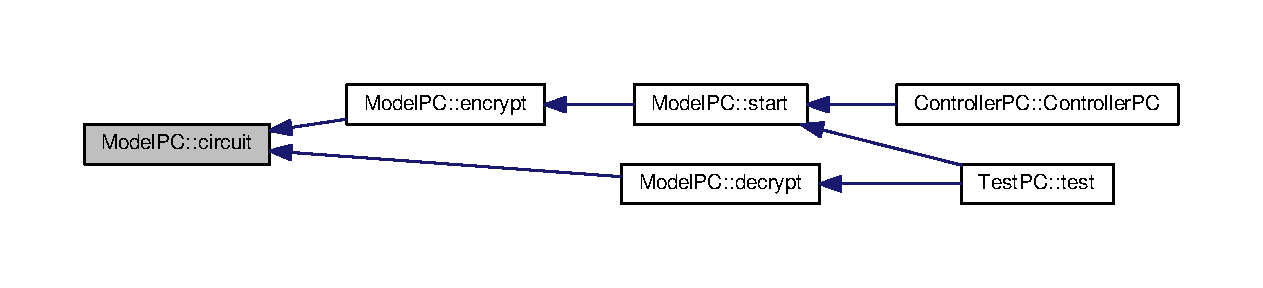
\includegraphics[width=350pt]{class_model_p_c_a1d0091062a0c836b283ec2f67411623b_icgraph}
\end{center}
\end{figure}


\index{Model\+PC@{Model\+PC}!Decrypt@{Decrypt}}
\index{Decrypt@{Decrypt}!Model\+PC@{Model\+PC}}
\subsubsection[{\texorpdfstring{Decrypt(\+Q\+Image $\ast$image, Q\+String key, int \+\_\+mode=0, Q\+String $\ast$\+\_\+error=nullptr)}{Decrypt(QImage *image, QString key, int _mode=0, QString *_error=nullptr)}}]{\setlength{\rightskip}{0pt plus 5cm}Q\+Byte\+Array Model\+P\+C\+::\+Decrypt (
\begin{DoxyParamCaption}
\item[{Q\+Image $\ast$}]{image, }
\item[{Q\+String}]{key, }
\item[{int}]{\+\_\+mode = {\ttfamily 0}, }
\item[{Q\+String $\ast$}]{\+\_\+error = {\ttfamily nullptr}}
\end{DoxyParamCaption}
)\hspace{0.3cm}{\ttfamily [static]}}\hypertarget{class_model_p_c_a902abaea4f07995b48c0f2fea6eceb7c}{}\label{class_model_p_c_a902abaea4f07995b48c0f2fea6eceb7c}


Definition at line \hyperlink{modelpc_8cpp_source_l00034}{34} of file \hyperlink{modelpc_8cpp_source}{modelpc.\+cpp}.



Here is the call graph for this function\+:
\nopagebreak
\begin{figure}[H]
\begin{center}
\leavevmode
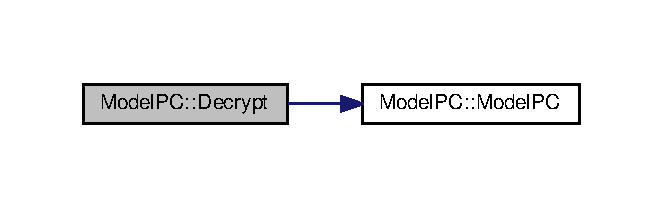
\includegraphics[width=318pt]{class_model_p_c_a902abaea4f07995b48c0f2fea6eceb7c_cgraph}
\end{center}
\end{figure}


\index{Model\+PC@{Model\+PC}!decrypt@{decrypt}}
\index{decrypt@{decrypt}!Model\+PC@{Model\+PC}}
\subsubsection[{\texorpdfstring{decrypt}{decrypt}}]{\setlength{\rightskip}{0pt plus 5cm}Q\+Byte\+Array Model\+P\+C\+::decrypt (
\begin{DoxyParamCaption}
\item[{Q\+Image $\ast$}]{image, }
\item[{Q\+String}]{key, }
\item[{int}]{\+\_\+mode = {\ttfamily 0}, }
\item[{Q\+String $\ast$}]{\+\_\+error = {\ttfamily nullptr}}
\end{DoxyParamCaption}
)\hspace{0.3cm}{\ttfamily [slot]}}\hypertarget{class_model_p_c_a5995215a34a1e1f504035715a8013809}{}\label{class_model_p_c_a5995215a34a1e1f504035715a8013809}


\hyperlink{class_model_p_c_a5995215a34a1e1f504035715a8013809}{Model\+P\+C\+::decrypt} Slot to be called when decrypt mode in \hyperlink{class_view_p_c}{View\+PC} is selected and started. 


\begin{DoxyParams}{Parameters}
{\em image} & Image to be decrypted. \\
\hline
{\em key} & Keyphrase with which the data is injected \\
\hline
{\em \+\_\+mode} & Mode for decryption \\
\hline
{\em \+\_\+error} & Error output \\
\hline
\end{DoxyParams}
\begin{DoxyReturn}{Returns}
Returns decrypted data 
\end{DoxyReturn}
\begin{DoxySeeAlso}{See also}
\hyperlink{class_view_p_c_a456d75b7c5d3a089302a576e7359f1f4}{View\+P\+C\+::on\+\_\+start\+Button\+\_\+clicked}, \hyperlink{class_model_p_c_aada6a04d81ada8f2b4ba18108c8d6f10}{Model\+P\+C\+::inject}, \hyperlink{class_model_p_c_a1d0091062a0c836b283ec2f67411623b}{Model\+P\+C\+::circuit} 
\end{DoxySeeAlso}


Definition at line \hyperlink{modelpc_8cpp_source_l00213}{213} of file \hyperlink{modelpc_8cpp_source}{modelpc.\+cpp}.



Here is the call graph for this function\+:
\nopagebreak
\begin{figure}[H]
\begin{center}
\leavevmode
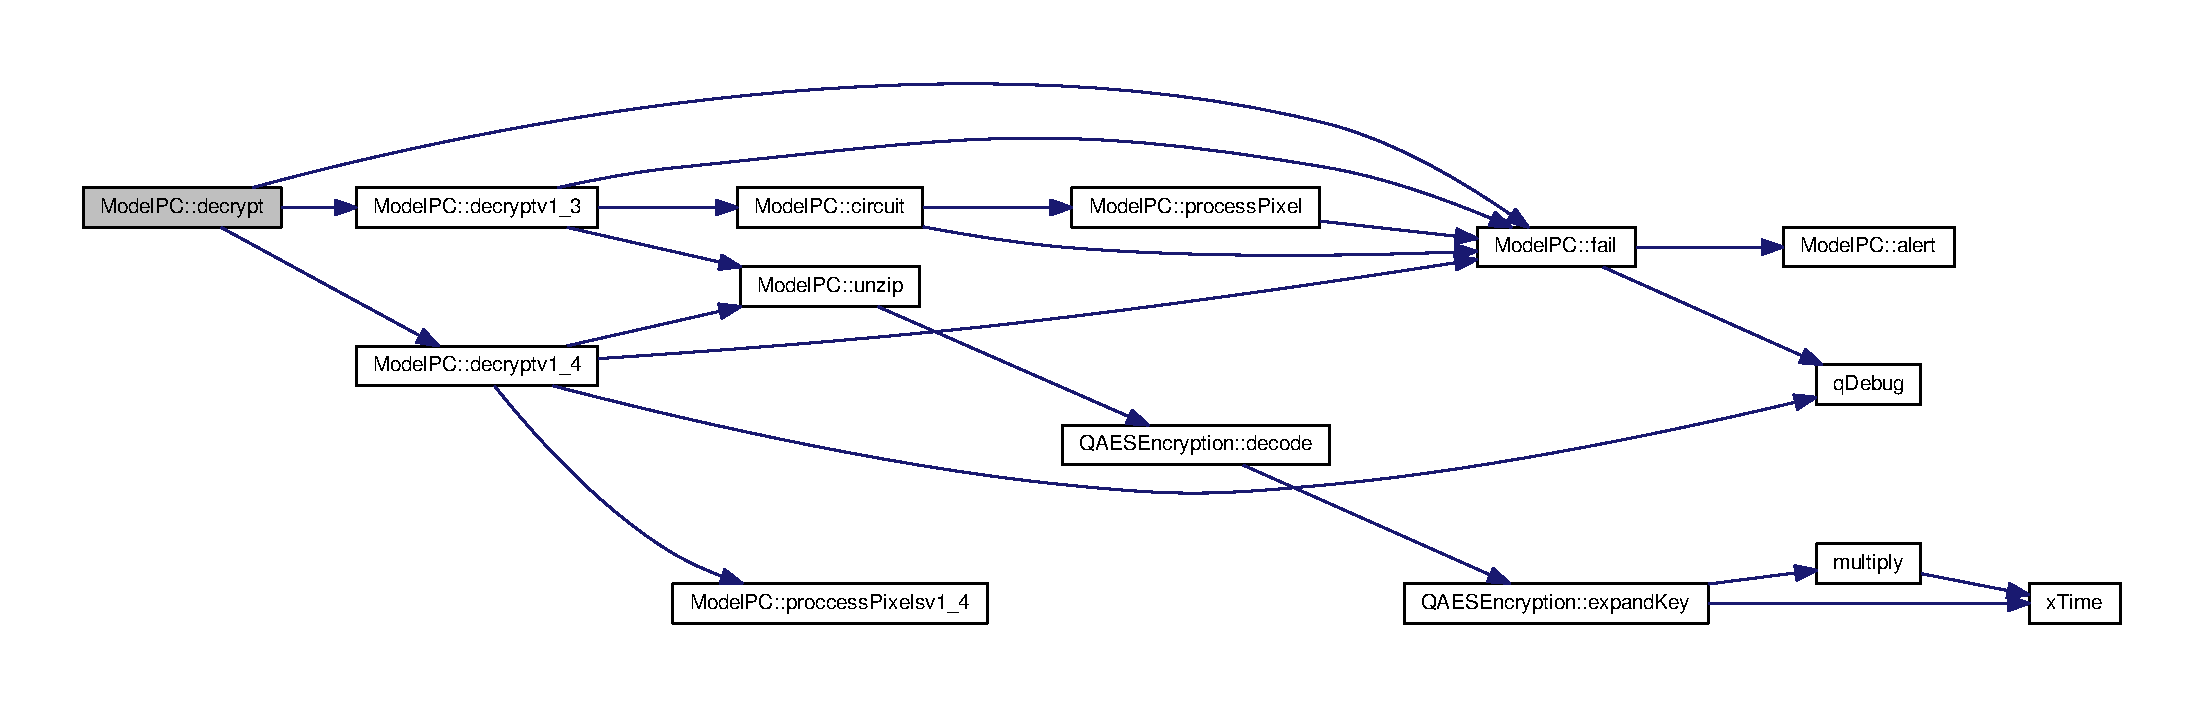
\includegraphics[width=350pt]{class_model_p_c_a5995215a34a1e1f504035715a8013809_cgraph}
\end{center}
\end{figure}


\index{Model\+PC@{Model\+PC}!decryptv1\+\_\+3@{decryptv1\+\_\+3}}
\index{decryptv1\+\_\+3@{decryptv1\+\_\+3}!Model\+PC@{Model\+PC}}
\subsubsection[{\texorpdfstring{decryptv1\+\_\+3(\+Q\+Image $\ast$image, Q\+String key)}{decryptv1_3(QImage *image, QString key)}}]{\setlength{\rightskip}{0pt plus 5cm}Q\+Byte\+Array Model\+P\+C\+::decryptv1\+\_\+3 (
\begin{DoxyParamCaption}
\item[{Q\+Image $\ast$}]{image, }
\item[{Q\+String}]{key}
\end{DoxyParamCaption}
)\hspace{0.3cm}{\ttfamily [protected]}}\hypertarget{class_model_p_c_a4fe70ebbedfaf31d45a35f82d0f06caa}{}\label{class_model_p_c_a4fe70ebbedfaf31d45a35f82d0f06caa}


\hyperlink{class_model_p_c_a4fe70ebbedfaf31d45a35f82d0f06caa}{Model\+P\+C\+::decryptv1\+\_\+3} Decrytps data from image in v1.\+3. 


\begin{DoxyParams}{Parameters}
{\em image} & Image with data \\
\hline
{\em key} & Key \\
\hline
\end{DoxyParams}
\begin{DoxyReturn}{Returns}
Returns obtained data 
\end{DoxyReturn}


Definition at line \hyperlink{modelpc_8cpp_source_l00774}{774} of file \hyperlink{modelpc_8cpp_source}{modelpc.\+cpp}.



Here is the call graph for this function\+:
\nopagebreak
\begin{figure}[H]
\begin{center}
\leavevmode
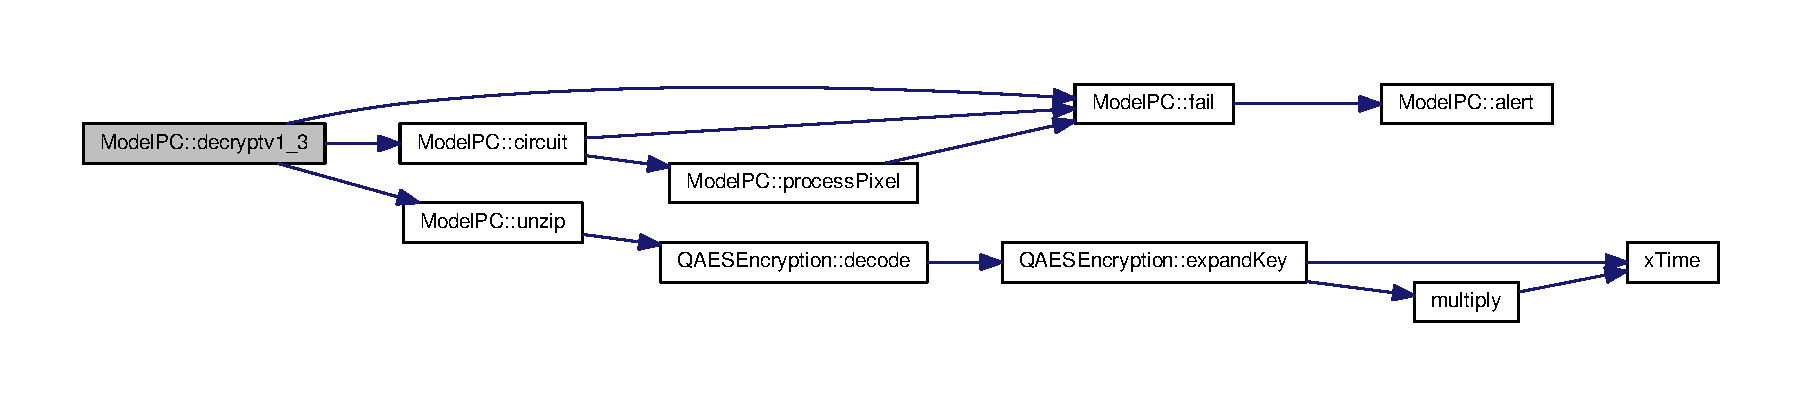
\includegraphics[width=350pt]{class_model_p_c_a4fe70ebbedfaf31d45a35f82d0f06caa_cgraph}
\end{center}
\end{figure}




Here is the caller graph for this function\+:
\nopagebreak
\begin{figure}[H]
\begin{center}
\leavevmode
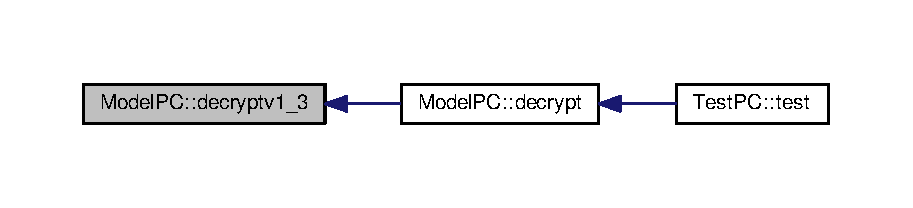
\includegraphics[width=327pt]{class_model_p_c_a4fe70ebbedfaf31d45a35f82d0f06caa_icgraph}
\end{center}
\end{figure}


\index{Model\+PC@{Model\+PC}!decryptv1\+\_\+4@{decryptv1\+\_\+4}}
\index{decryptv1\+\_\+4@{decryptv1\+\_\+4}!Model\+PC@{Model\+PC}}
\subsubsection[{\texorpdfstring{decryptv1\+\_\+4(\+Q\+Image $\ast$image, Q\+String key)}{decryptv1_4(QImage *image, QString key)}}]{\setlength{\rightskip}{0pt plus 5cm}Q\+Byte\+Array Model\+P\+C\+::decryptv1\+\_\+4 (
\begin{DoxyParamCaption}
\item[{Q\+Image $\ast$}]{image, }
\item[{Q\+String}]{key}
\end{DoxyParamCaption}
)\hspace{0.3cm}{\ttfamily [protected]}}\hypertarget{class_model_p_c_a7a1f7d491e1bde16936190b9e90896b0}{}\label{class_model_p_c_a7a1f7d491e1bde16936190b9e90896b0}


\hyperlink{class_model_p_c_a7a1f7d491e1bde16936190b9e90896b0}{Model\+P\+C\+::decryptv1\+\_\+4} Decrypts data from image in v1.\+4+. 


\begin{DoxyParams}{Parameters}
{\em image} & Image with data \\
\hline
{\em key} & Key \\
\hline
\end{DoxyParams}
\begin{DoxyReturn}{Returns}
Returns obtained data 
\end{DoxyReturn}


Definition at line \hyperlink{modelpc_8cpp_source_l00599}{599} of file \hyperlink{modelpc_8cpp_source}{modelpc.\+cpp}.



Here is the call graph for this function\+:
\nopagebreak
\begin{figure}[H]
\begin{center}
\leavevmode
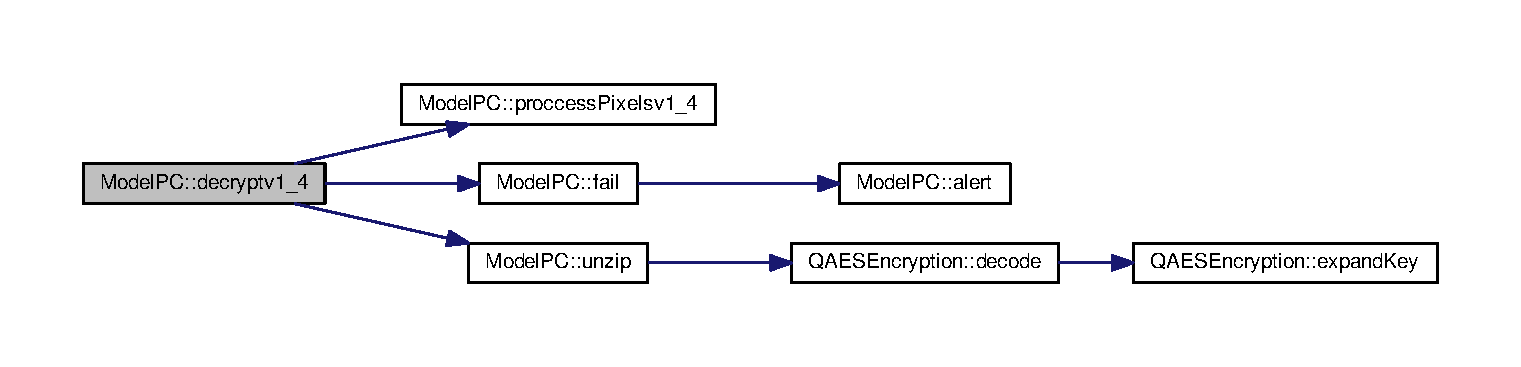
\includegraphics[width=350pt]{class_model_p_c_a7a1f7d491e1bde16936190b9e90896b0_cgraph}
\end{center}
\end{figure}




Here is the caller graph for this function\+:
\nopagebreak
\begin{figure}[H]
\begin{center}
\leavevmode
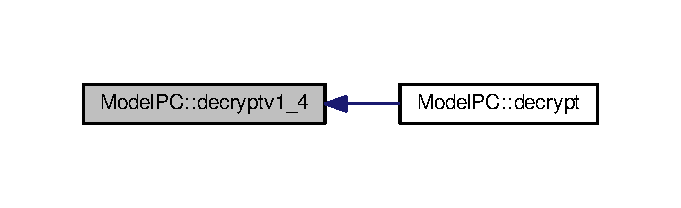
\includegraphics[width=327pt]{class_model_p_c_a7a1f7d491e1bde16936190b9e90896b0_icgraph}
\end{center}
\end{figure}


\index{Model\+PC@{Model\+PC}!Encrypt@{Encrypt}}
\index{Encrypt@{Encrypt}!Model\+PC@{Model\+PC}}
\subsubsection[{\texorpdfstring{Encrypt(\+Q\+Byte\+Array data, Q\+Image $\ast$image, int \+\_\+mode, Q\+String key="""", int \+\_\+bits\+Used=8, Q\+String $\ast$\+\_\+error=nullptr)}{Encrypt(QByteArray data, QImage *image, int _mode, QString key="", int _bitsUsed=8, QString *_error=nullptr)}}]{\setlength{\rightskip}{0pt plus 5cm}Q\+Image $\ast$ Model\+P\+C\+::\+Encrypt (
\begin{DoxyParamCaption}
\item[{Q\+Byte\+Array}]{data, }
\item[{Q\+Image $\ast$}]{image, }
\item[{int}]{\+\_\+mode, }
\item[{Q\+String}]{key = {\ttfamily \char`\"{}\char`\"{}}, }
\item[{int}]{\+\_\+bits\+Used = {\ttfamily 8}, }
\item[{Q\+String $\ast$}]{\+\_\+error = {\ttfamily nullptr}}
\end{DoxyParamCaption}
)\hspace{0.3cm}{\ttfamily [static]}}\hypertarget{class_model_p_c_a271cf9285e32df58ffbfc918e6482bbd}{}\label{class_model_p_c_a271cf9285e32df58ffbfc918e6482bbd}


Definition at line \hyperlink{modelpc_8cpp_source_l00024}{24} of file \hyperlink{modelpc_8cpp_source}{modelpc.\+cpp}.



Here is the call graph for this function\+:
\nopagebreak
\begin{figure}[H]
\begin{center}
\leavevmode
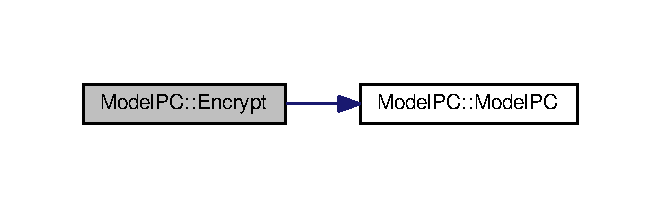
\includegraphics[width=317pt]{class_model_p_c_a271cf9285e32df58ffbfc918e6482bbd_cgraph}
\end{center}
\end{figure}


\index{Model\+PC@{Model\+PC}!encrypt@{encrypt}}
\index{encrypt@{encrypt}!Model\+PC@{Model\+PC}}
\subsubsection[{\texorpdfstring{encrypt}{encrypt}}]{\setlength{\rightskip}{0pt plus 5cm}Q\+Image $\ast$ Model\+P\+C\+::encrypt (
\begin{DoxyParamCaption}
\item[{Q\+Byte\+Array}]{data, }
\item[{Q\+Image $\ast$}]{image, }
\item[{int}]{\+\_\+mode, }
\item[{Q\+String}]{key = {\ttfamily \char`\"{}\char`\"{}}, }
\item[{int}]{\+\_\+bits\+Used = {\ttfamily 8}, }
\item[{Q\+String $\ast$}]{\+\_\+error = {\ttfamily nullptr}}
\end{DoxyParamCaption}
)\hspace{0.3cm}{\ttfamily [slot]}}\hypertarget{class_model_p_c_a6f191f62d4635d0d3555fcc0be298794}{}\label{class_model_p_c_a6f191f62d4635d0d3555fcc0be298794}


\hyperlink{class_model_p_c_a6f191f62d4635d0d3555fcc0be298794}{Model\+P\+C\+::encrypt} Slot to zip and inject data and provide it with some extra stuff After completion start standard \hyperlink{class_model_p_c_aada6a04d81ada8f2b4ba18108c8d6f10}{Model\+P\+C\+::inject} Isn\textquotesingle{}t used in Picture\+Crypt, but used can be used in other -\/ custom projects. 


\begin{DoxyParams}{Parameters}
{\em data} & Data for embedding \\
\hline
{\em image} & Image for embedding \\
\hline
{\em mode} & Mode for embedding \\
\hline
{\em key} & Key for extra encryption \\
\hline
{\em \+\_\+bits\+Used} & Bits per byte (see Model\+P\+C\+::bits\+Used) \\
\hline
{\em \+\_\+error} & Error output \\
\hline
\end{DoxyParams}
\begin{DoxyReturn}{Returns}
Returns image with embedded data 
\end{DoxyReturn}
\begin{DoxySeeAlso}{See also}
\hyperlink{class_model_p_c_aada6a04d81ada8f2b4ba18108c8d6f10}{Model\+P\+C\+::inject} 
\end{DoxySeeAlso}


Definition at line \hyperlink{modelpc_8cpp_source_l00051}{51} of file \hyperlink{modelpc_8cpp_source}{modelpc.\+cpp}.



Here is the call graph for this function\+:
\nopagebreak
\begin{figure}[H]
\begin{center}
\leavevmode
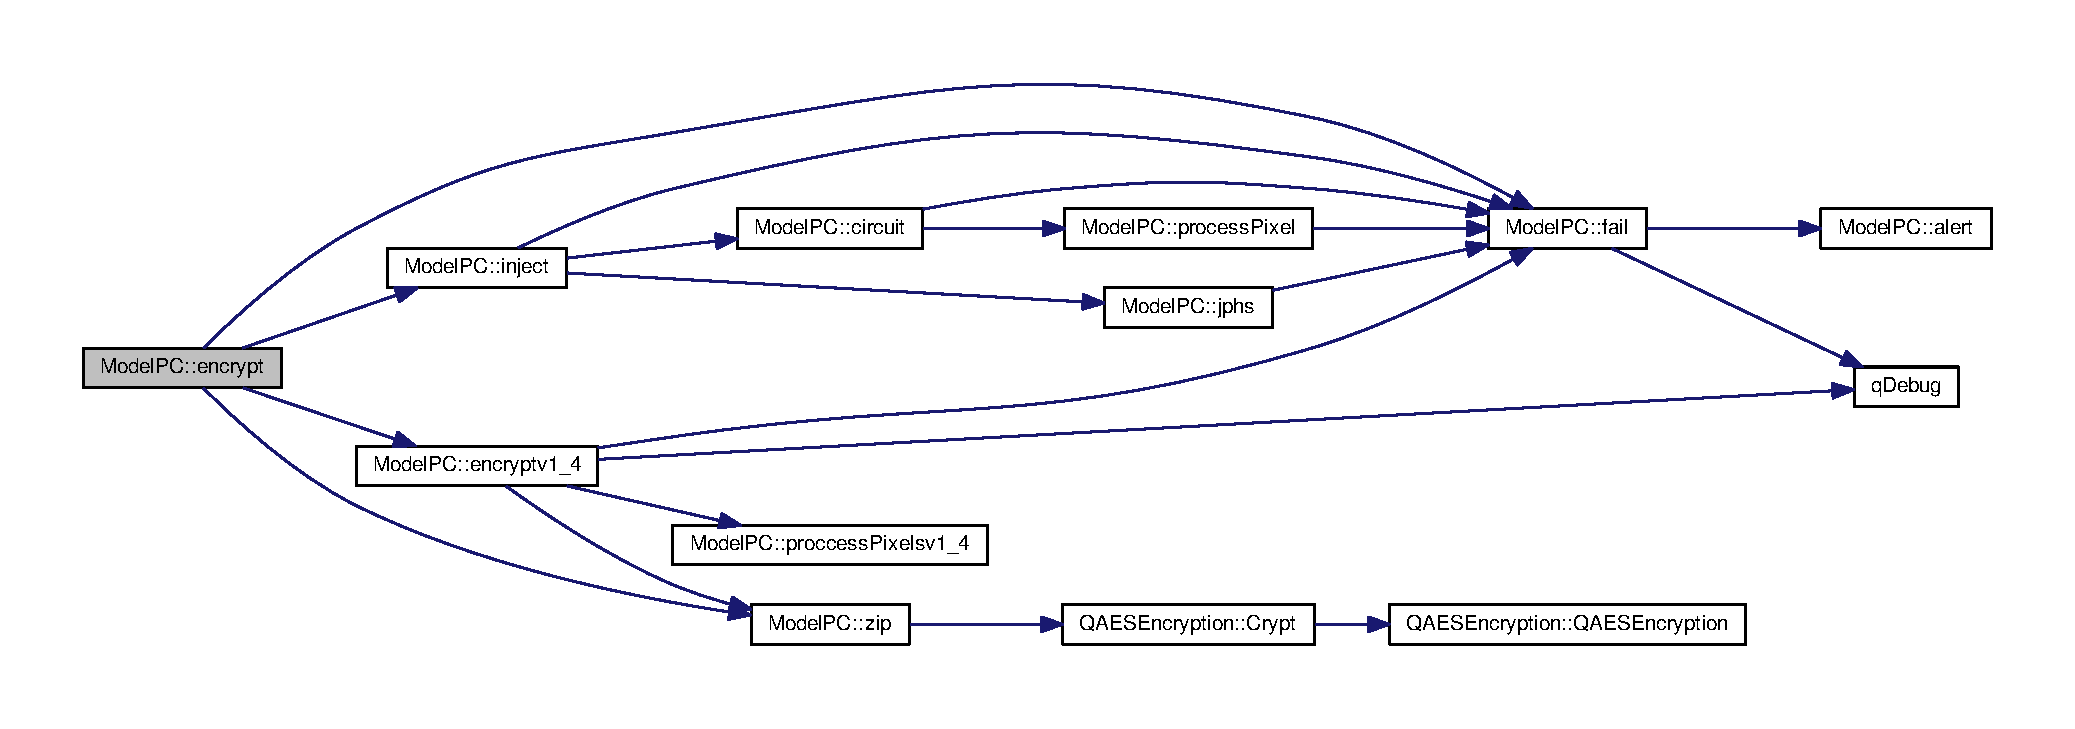
\includegraphics[width=350pt]{class_model_p_c_a6f191f62d4635d0d3555fcc0be298794_cgraph}
\end{center}
\end{figure}


\index{Model\+PC@{Model\+PC}!encryptv1\+\_\+4@{encryptv1\+\_\+4}}
\index{encryptv1\+\_\+4@{encryptv1\+\_\+4}!Model\+PC@{Model\+PC}}
\subsubsection[{\texorpdfstring{encryptv1\+\_\+4(\+Q\+Image $\ast$image, Q\+Byte\+Array data, Q\+String key)}{encryptv1_4(QImage *image, QByteArray data, QString key)}}]{\setlength{\rightskip}{0pt plus 5cm}void Model\+P\+C\+::encryptv1\+\_\+4 (
\begin{DoxyParamCaption}
\item[{Q\+Image $\ast$}]{image, }
\item[{Q\+Byte\+Array}]{data, }
\item[{Q\+String}]{key}
\end{DoxyParamCaption}
)\hspace{0.3cm}{\ttfamily [protected]}}\hypertarget{class_model_p_c_a4daefc3fb87a1f19172b9b20c987eb12}{}\label{class_model_p_c_a4daefc3fb87a1f19172b9b20c987eb12}


\hyperlink{class_model_p_c_a4daefc3fb87a1f19172b9b20c987eb12}{Model\+P\+C\+::encryptv1\+\_\+4} Encrypts and injects data to image used in v1.\+4+. 


\begin{DoxyParams}{Parameters}
{\em image} & Image for injecting \\
\hline
{\em data} & Data for embedding \\
\hline
\end{DoxyParams}


Definition at line \hyperlink{modelpc_8cpp_source_l00557}{557} of file \hyperlink{modelpc_8cpp_source}{modelpc.\+cpp}.



Here is the call graph for this function\+:
\nopagebreak
\begin{figure}[H]
\begin{center}
\leavevmode
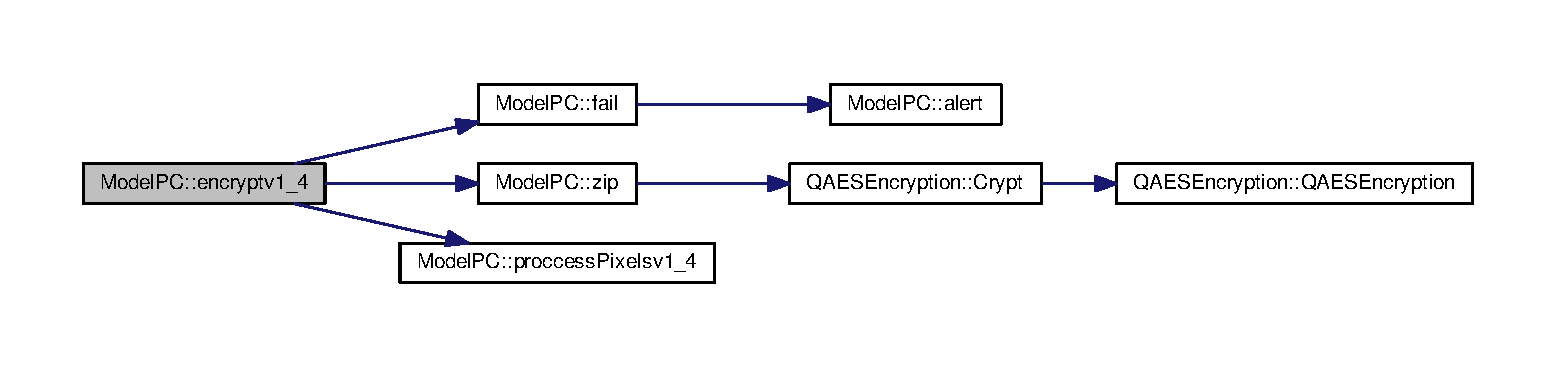
\includegraphics[width=350pt]{class_model_p_c_a4daefc3fb87a1f19172b9b20c987eb12_cgraph}
\end{center}
\end{figure}




Here is the caller graph for this function\+:
\nopagebreak
\begin{figure}[H]
\begin{center}
\leavevmode
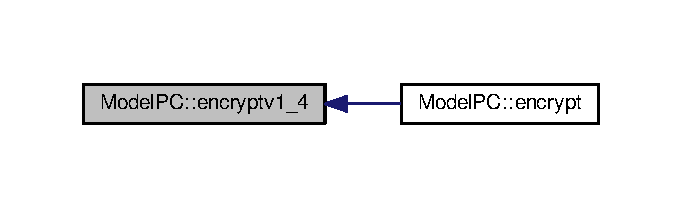
\includegraphics[width=327pt]{class_model_p_c_a4daefc3fb87a1f19172b9b20c987eb12_icgraph}
\end{center}
\end{figure}


\index{Model\+PC@{Model\+PC}!fail@{fail}}
\index{fail@{fail}!Model\+PC@{Model\+PC}}
\subsubsection[{\texorpdfstring{fail}{fail}}]{\setlength{\rightskip}{0pt plus 5cm}void Model\+P\+C\+::fail (
\begin{DoxyParamCaption}
\item[{Q\+String}]{message}
\end{DoxyParamCaption}
)\hspace{0.3cm}{\ttfamily [slot]}}\hypertarget{class_model_p_c_a47464b59b7e37fcee25e55475708aabd}{}\label{class_model_p_c_a47464b59b7e37fcee25e55475708aabd}


\hyperlink{class_model_p_c_a47464b59b7e37fcee25e55475708aabd}{Model\+P\+C\+::fail} Slot to stop execution of cryption. 


\begin{DoxyParams}{Parameters}
{\em message} & Message for user \\
\hline
\end{DoxyParams}


Definition at line \hyperlink{modelpc_8cpp_source_l00280}{280} of file \hyperlink{modelpc_8cpp_source}{modelpc.\+cpp}.



Here is the call graph for this function\+:
\nopagebreak
\begin{figure}[H]
\begin{center}
\leavevmode
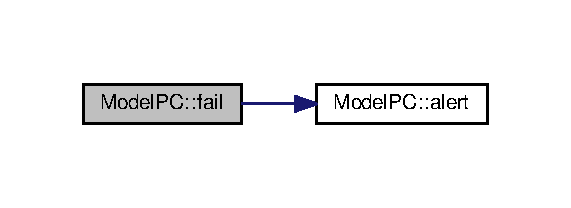
\includegraphics[width=274pt]{class_model_p_c_a47464b59b7e37fcee25e55475708aabd_cgraph}
\end{center}
\end{figure}




Here is the caller graph for this function\+:
\nopagebreak
\begin{figure}[H]
\begin{center}
\leavevmode
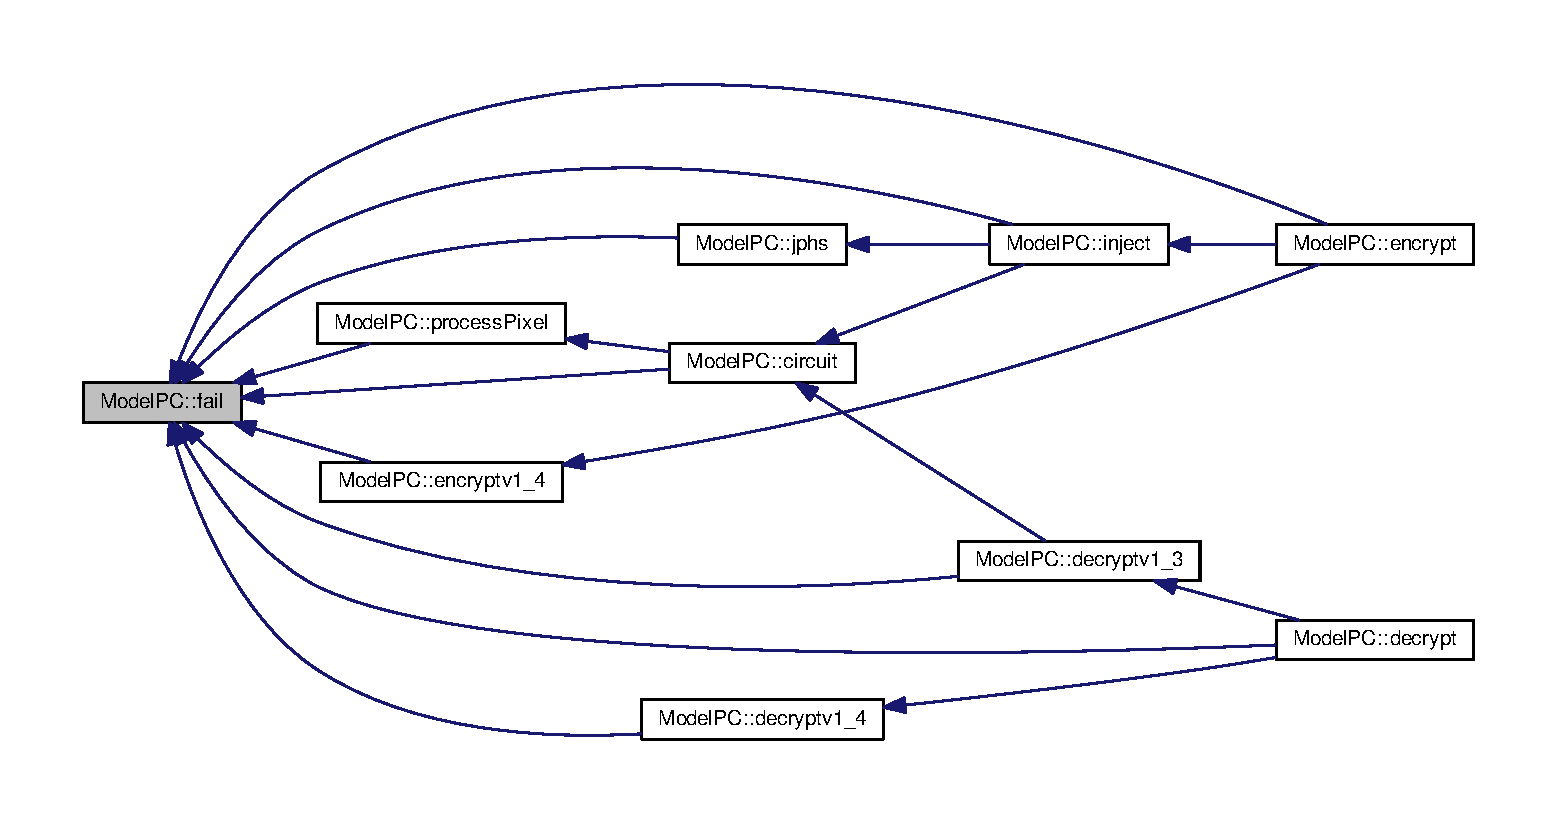
\includegraphics[width=350pt]{class_model_p_c_a47464b59b7e37fcee25e55475708aabd_icgraph}
\end{center}
\end{figure}


\index{Model\+PC@{Model\+PC}!Inject@{Inject}}
\index{Inject@{Inject}!Model\+PC@{Model\+PC}}
\subsubsection[{\texorpdfstring{Inject(\+Q\+Byte\+Array encr\+\_\+data, Q\+Image $\ast$image, int \+\_\+mode, int \+\_\+bits\+Used=8, Q\+String $\ast$\+\_\+error=nullptr)}{Inject(QByteArray encr_data, QImage *image, int _mode, int _bitsUsed=8, QString *_error=nullptr)}}]{\setlength{\rightskip}{0pt plus 5cm}Q\+Image $\ast$ Model\+P\+C\+::\+Inject (
\begin{DoxyParamCaption}
\item[{Q\+Byte\+Array}]{encr\+\_\+data, }
\item[{Q\+Image $\ast$}]{image, }
\item[{int}]{\+\_\+mode, }
\item[{int}]{\+\_\+bits\+Used = {\ttfamily 8}, }
\item[{Q\+String $\ast$}]{\+\_\+error = {\ttfamily nullptr}}
\end{DoxyParamCaption}
)\hspace{0.3cm}{\ttfamily [static]}}\hypertarget{class_model_p_c_ac17e68e6aab134621b0d151d74acdc82}{}\label{class_model_p_c_ac17e68e6aab134621b0d151d74acdc82}


Definition at line \hyperlink{modelpc_8cpp_source_l00029}{29} of file \hyperlink{modelpc_8cpp_source}{modelpc.\+cpp}.



Here is the call graph for this function\+:
\nopagebreak
\begin{figure}[H]
\begin{center}
\leavevmode
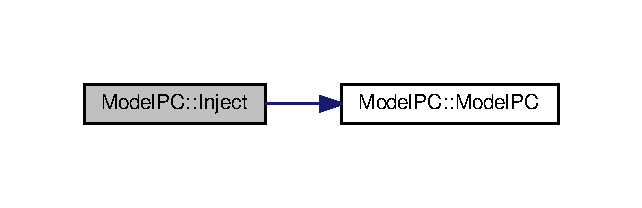
\includegraphics[width=307pt]{class_model_p_c_ac17e68e6aab134621b0d151d74acdc82_cgraph}
\end{center}
\end{figure}


\index{Model\+PC@{Model\+PC}!inject@{inject}}
\index{inject@{inject}!Model\+PC@{Model\+PC}}
\subsubsection[{\texorpdfstring{inject}{inject}}]{\setlength{\rightskip}{0pt plus 5cm}Q\+Image $\ast$ Model\+P\+C\+::inject (
\begin{DoxyParamCaption}
\item[{Q\+Byte\+Array}]{encr\+\_\+data, }
\item[{Q\+Image $\ast$}]{image, }
\item[{int}]{\+\_\+mode, }
\item[{int}]{\+\_\+bits\+Used = {\ttfamily 8}, }
\item[{Q\+String $\ast$}]{\+\_\+error = {\ttfamily nullptr}}
\end{DoxyParamCaption}
)\hspace{0.3cm}{\ttfamily [slot]}}\hypertarget{class_model_p_c_aada6a04d81ada8f2b4ba18108c8d6f10}{}\label{class_model_p_c_aada6a04d81ada8f2b4ba18108c8d6f10}


\hyperlink{class_model_p_c_aada6a04d81ada8f2b4ba18108c8d6f10}{Model\+P\+C\+::inject} Slot to be called when encrypt mode in \hyperlink{class_view_p_c}{View\+PC} is selected and started. 


\begin{DoxyParams}{Parameters}
{\em encr\+\_\+data} & Data to be inserted to an image. \\
\hline
{\em image} & Image to be inserted in. \\
\hline
{\em mode} & Mode of encryption \\
\hline
{\em \+\_\+bits\+Used} & Bits per byte used \\
\hline
{\em \+\_\+error} & Error output \\
\hline
\end{DoxyParams}
\begin{DoxyReturn}{Returns}
Returns image with embedded data. 
\end{DoxyReturn}
\begin{DoxySeeAlso}{See also}
\hyperlink{class_view_p_c_a456d75b7c5d3a089302a576e7359f1f4}{View\+P\+C\+::on\+\_\+start\+Button\+\_\+clicked}, \hyperlink{class_model_p_c_a5995215a34a1e1f504035715a8013809}{Model\+P\+C\+::decrypt}, \hyperlink{class_model_p_c_a1d0091062a0c836b283ec2f67411623b}{Model\+P\+C\+::circuit}, Model\+P\+C\+::start 
\end{DoxySeeAlso}


Definition at line \hyperlink{modelpc_8cpp_source_l00139}{139} of file \hyperlink{modelpc_8cpp_source}{modelpc.\+cpp}.



Here is the call graph for this function\+:
\nopagebreak
\begin{figure}[H]
\begin{center}
\leavevmode
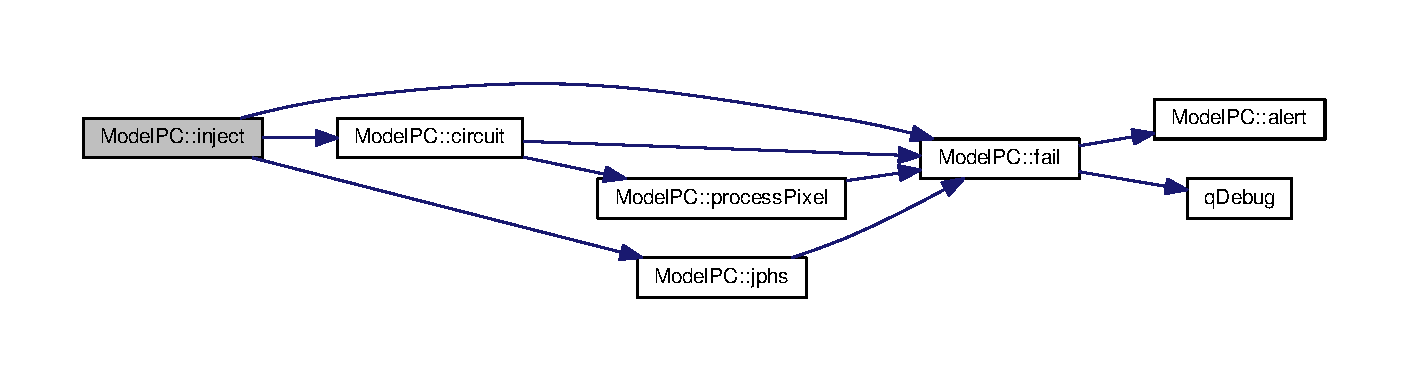
\includegraphics[width=350pt]{class_model_p_c_aada6a04d81ada8f2b4ba18108c8d6f10_cgraph}
\end{center}
\end{figure}




Here is the caller graph for this function\+:
\nopagebreak
\begin{figure}[H]
\begin{center}
\leavevmode
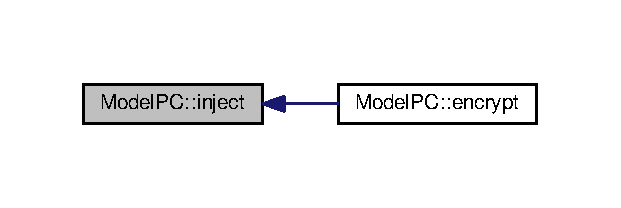
\includegraphics[width=297pt]{class_model_p_c_aada6a04d81ada8f2b4ba18108c8d6f10_icgraph}
\end{center}
\end{figure}


\index{Model\+PC@{Model\+PC}!jphs@{jphs}}
\index{jphs@{jphs}!Model\+PC@{Model\+PC}}
\subsubsection[{\texorpdfstring{jphs(\+Q\+Image $\ast$image, Q\+Byte\+Array $\ast$data)}{jphs(QImage *image, QByteArray *data)}}]{\setlength{\rightskip}{0pt plus 5cm}void Model\+P\+C\+::jphs (
\begin{DoxyParamCaption}
\item[{Q\+Image $\ast$}]{image, }
\item[{Q\+Byte\+Array $\ast$}]{data}
\end{DoxyParamCaption}
)\hspace{0.3cm}{\ttfamily [protected]}}\hypertarget{class_model_p_c_a8bee0255c09449868c7e6097afaaf0cd}{}\label{class_model_p_c_a8bee0255c09449868c7e6097afaaf0cd}


\hyperlink{class_model_p_c_a8bee0255c09449868c7e6097afaaf0cd}{Model\+P\+C\+::jphs} J\+P\+HS function to use jphide and jpseek (currently under development) 


\begin{DoxyParams}{Parameters}
{\em image} & Image for embedding \\
\hline
{\em data} & Data \\
\hline
\end{DoxyParams}


Definition at line \hyperlink{modelpc_8cpp_source_l00295}{295} of file \hyperlink{modelpc_8cpp_source}{modelpc.\+cpp}.



Here is the call graph for this function\+:
\nopagebreak
\begin{figure}[H]
\begin{center}
\leavevmode
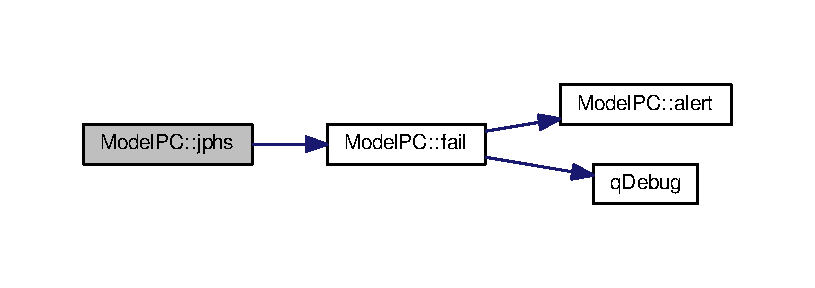
\includegraphics[width=350pt]{class_model_p_c_a8bee0255c09449868c7e6097afaaf0cd_cgraph}
\end{center}
\end{figure}




Here is the caller graph for this function\+:
\nopagebreak
\begin{figure}[H]
\begin{center}
\leavevmode
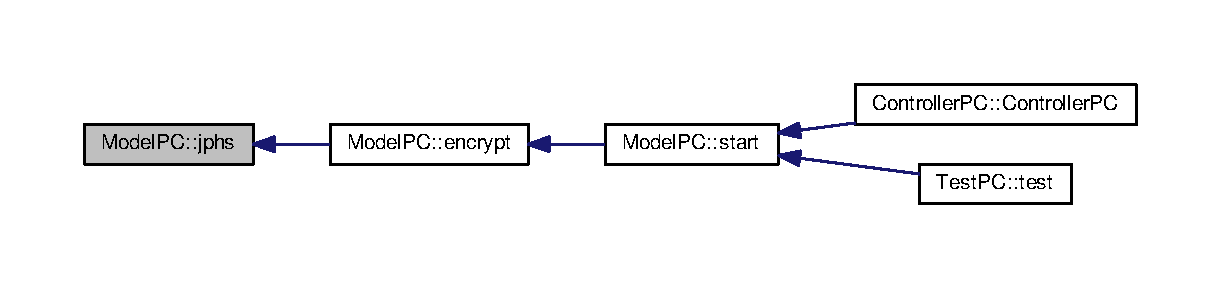
\includegraphics[width=350pt]{class_model_p_c_a8bee0255c09449868c7e6097afaaf0cd_icgraph}
\end{center}
\end{figure}


\index{Model\+PC@{Model\+PC}!proccess\+Pixelsv1\+\_\+4@{proccess\+Pixelsv1\+\_\+4}}
\index{proccess\+Pixelsv1\+\_\+4@{proccess\+Pixelsv1\+\_\+4}!Model\+PC@{Model\+PC}}
\subsubsection[{\texorpdfstring{proccess\+Pixelsv1\+\_\+4(\+Q\+Image $\ast$image, Q\+Byte\+Array $\ast$data, Q\+Byte\+Array key, bool is\+Encrypt, Q\+Vector$<$ Q\+Pair$<$ Q\+Point, Q\+Pair$<$ int, int $>$ $>$ $>$ $\ast$were, long long size=-\/1)}{proccessPixelsv1_4(QImage *image, QByteArray *data, QByteArray key, bool isEncrypt, QVector< QPair< QPoint, QPair< int, int > > > *were, long long size=-1)}}]{\setlength{\rightskip}{0pt plus 5cm}void Model\+P\+C\+::proccess\+Pixelsv1\+\_\+4 (
\begin{DoxyParamCaption}
\item[{Q\+Image $\ast$}]{image, }
\item[{Q\+Byte\+Array $\ast$}]{data, }
\item[{Q\+Byte\+Array}]{key, }
\item[{bool}]{is\+Encrypt, }
\item[{Q\+Vector$<$ Q\+Pair$<$ Q\+Point, Q\+Pair$<$ int, int $>$ $>$ $>$ $\ast$}]{were, }
\item[{long long}]{size = {\ttfamily -\/1}}
\end{DoxyParamCaption}
)\hspace{0.3cm}{\ttfamily [protected]}}\hypertarget{class_model_p_c_a5cdb4d1d61ff62ee9d45b496a7dbf1fb}{}\label{class_model_p_c_a5cdb4d1d61ff62ee9d45b496a7dbf1fb}


\hyperlink{class_model_p_c_a5cdb4d1d61ff62ee9d45b496a7dbf1fb}{Model\+P\+C\+::proccess\+Pixelsv1\+\_\+4} Hides (or retrieves) data to/from pixels. 


\begin{DoxyParams}{Parameters}
{\em image} & Original image \\
\hline
{\em data} & Data to write (Pointer to empty Q\+Byte\+Array if decrypting) \\
\hline
{\em key} & Key \\
\hline
{\em is\+Encrypt} & Mode of Cryption (true -\/$>$ encryption, false -\/$>$ decryption) \\
\hline
{\em were} & Were vector for visited pixels \\
\hline
{\em size} & Size of reading data, unneeded if writing \\
\hline
\end{DoxyParams}


Definition at line \hyperlink{modelpc_8cpp_source_l00660}{660} of file \hyperlink{modelpc_8cpp_source}{modelpc.\+cpp}.



Here is the caller graph for this function\+:
\nopagebreak
\begin{figure}[H]
\begin{center}
\leavevmode
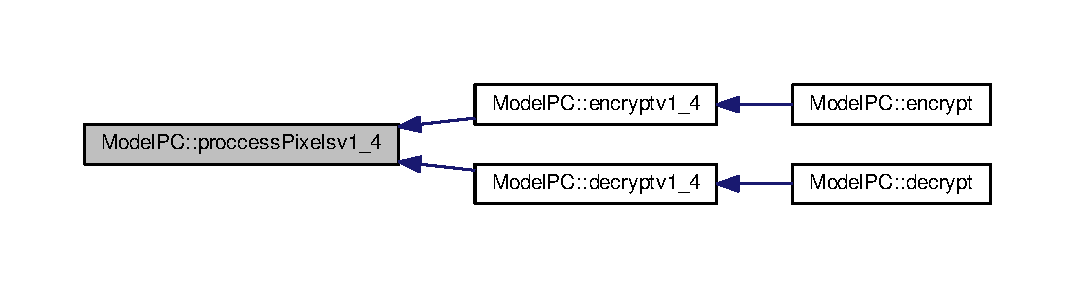
\includegraphics[width=350pt]{class_model_p_c_a5cdb4d1d61ff62ee9d45b496a7dbf1fb_icgraph}
\end{center}
\end{figure}


\index{Model\+PC@{Model\+PC}!process\+Pixel@{process\+Pixel}}
\index{process\+Pixel@{process\+Pixel}!Model\+PC@{Model\+PC}}
\subsubsection[{\texorpdfstring{process\+Pixel(\+Q\+Point pos, Q\+Vector$<$ Q\+Point $>$ $\ast$were, bool is\+Encrypt)}{processPixel(QPoint pos, QVector< QPoint > *were, bool isEncrypt)}}]{\setlength{\rightskip}{0pt plus 5cm}void Model\+P\+C\+::process\+Pixel (
\begin{DoxyParamCaption}
\item[{Q\+Point}]{pos, }
\item[{Q\+Vector$<$ Q\+Point $>$ $\ast$}]{were, }
\item[{bool}]{is\+Encrypt}
\end{DoxyParamCaption}
)\hspace{0.3cm}{\ttfamily [protected]}}\hypertarget{class_model_p_c_a1171f9fe1550133dc9053a46b4e5bcfd}{}\label{class_model_p_c_a1171f9fe1550133dc9053a46b4e5bcfd}


\hyperlink{class_model_p_c_a1171f9fe1550133dc9053a46b4e5bcfd}{Model\+P\+C\+::process\+Pixel} Processes every pixel. Reads its contains or writes data. 


\begin{DoxyParams}{Parameters}
{\em pos} & Position of pixel \\
\hline
{\em were} & Vector array containing pixels, that were already processed. \\
\hline
{\em is\+Encrypt} & Mode of operation. If true encryption operations will continue, else the decryption ones. \\
\hline
\end{DoxyParams}


Definition at line \hyperlink{modelpc_8cpp_source_l00497}{497} of file \hyperlink{modelpc_8cpp_source}{modelpc.\+cpp}.



Here is the call graph for this function\+:
\nopagebreak
\begin{figure}[H]
\begin{center}
\leavevmode
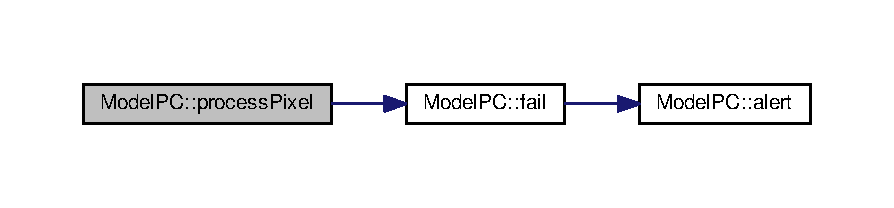
\includegraphics[width=350pt]{class_model_p_c_a1171f9fe1550133dc9053a46b4e5bcfd_cgraph}
\end{center}
\end{figure}




Here is the caller graph for this function\+:
\nopagebreak
\begin{figure}[H]
\begin{center}
\leavevmode
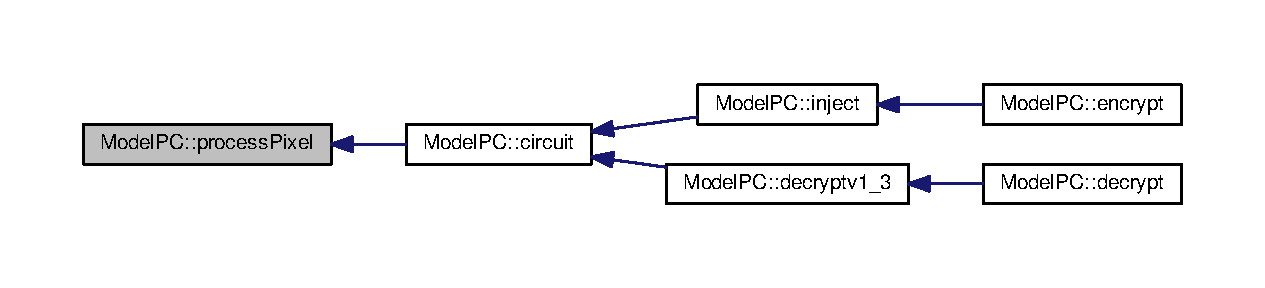
\includegraphics[width=350pt]{class_model_p_c_a1171f9fe1550133dc9053a46b4e5bcfd_icgraph}
\end{center}
\end{figure}


\index{Model\+PC@{Model\+PC}!save\+Data@{save\+Data}}
\index{save\+Data@{save\+Data}!Model\+PC@{Model\+PC}}
\subsubsection[{\texorpdfstring{save\+Data}{saveData}}]{\setlength{\rightskip}{0pt plus 5cm}void Model\+P\+C\+::save\+Data (
\begin{DoxyParamCaption}
\item[{Q\+Byte\+Array}]{data}
\end{DoxyParamCaption}
)\hspace{0.3cm}{\ttfamily [signal]}}\hypertarget{class_model_p_c_a0855107fb0ccc247cd9e893fae9bb08a}{}\label{class_model_p_c_a0855107fb0ccc247cd9e893fae9bb08a}


save\+Data Signal to be called to save data from \hyperlink{class_model_p_c_a5995215a34a1e1f504035715a8013809}{Model\+P\+C\+::decrypt}. 


\begin{DoxyParams}{Parameters}
{\em data} & Data to be saved. \\
\hline
\end{DoxyParams}


Here is the caller graph for this function\+:
\nopagebreak
\begin{figure}[H]
\begin{center}
\leavevmode
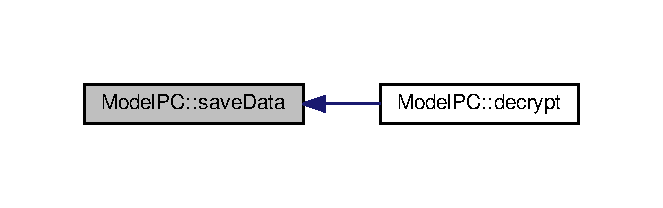
\includegraphics[width=316pt]{class_model_p_c_a0855107fb0ccc247cd9e893fae9bb08a_icgraph}
\end{center}
\end{figure}


\index{Model\+PC@{Model\+PC}!save\+Image@{save\+Image}}
\index{save\+Image@{save\+Image}!Model\+PC@{Model\+PC}}
\subsubsection[{\texorpdfstring{save\+Image}{saveImage}}]{\setlength{\rightskip}{0pt plus 5cm}void Model\+P\+C\+::save\+Image (
\begin{DoxyParamCaption}
\item[{Q\+Image $\ast$}]{image}
\end{DoxyParamCaption}
)\hspace{0.3cm}{\ttfamily [signal]}}\hypertarget{class_model_p_c_a41f5e2e8022679046e4d3fa1109025fa}{}\label{class_model_p_c_a41f5e2e8022679046e4d3fa1109025fa}


save\+Image Signal to be called to save image from \hyperlink{class_model_p_c_a6f191f62d4635d0d3555fcc0be298794}{Model\+P\+C\+::encrypt}. 


\begin{DoxyParams}{Parameters}
{\em image} & Image to be saved. \\
\hline
\end{DoxyParams}


Here is the caller graph for this function\+:
\nopagebreak
\begin{figure}[H]
\begin{center}
\leavevmode
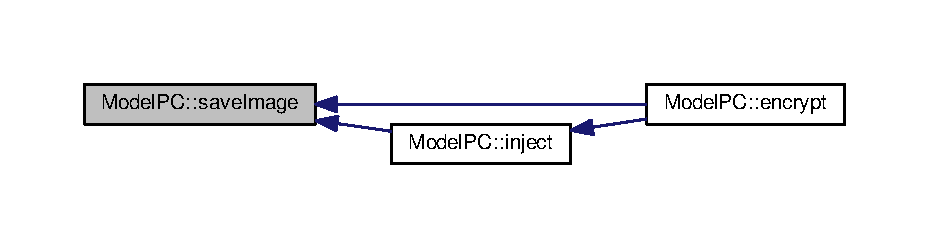
\includegraphics[width=350pt]{class_model_p_c_a41f5e2e8022679046e4d3fa1109025fa_icgraph}
\end{center}
\end{figure}


\index{Model\+PC@{Model\+PC}!set\+Progress@{set\+Progress}}
\index{set\+Progress@{set\+Progress}!Model\+PC@{Model\+PC}}
\subsubsection[{\texorpdfstring{set\+Progress}{setProgress}}]{\setlength{\rightskip}{0pt plus 5cm}void Model\+P\+C\+::set\+Progress (
\begin{DoxyParamCaption}
\item[{int}]{val}
\end{DoxyParamCaption}
)\hspace{0.3cm}{\ttfamily [signal]}}\hypertarget{class_model_p_c_afdcd80f0ed5062e145a71f09b0897547}{}\label{class_model_p_c_afdcd80f0ed5062e145a71f09b0897547}


set\+Progress Signal to be called to set progress of Progress\+Dialog. 


\begin{DoxyParams}{Parameters}
{\em val} & Value to be set. \\
\hline
\end{DoxyParams}
\begin{DoxySeeAlso}{See also}
\hyperlink{class_view_p_c_a9c32a1fdb6ead84e5ada8fba8860c7ed}{View\+P\+C\+::set\+Progress} 
\end{DoxySeeAlso}


Here is the caller graph for this function\+:
\nopagebreak
\begin{figure}[H]
\begin{center}
\leavevmode
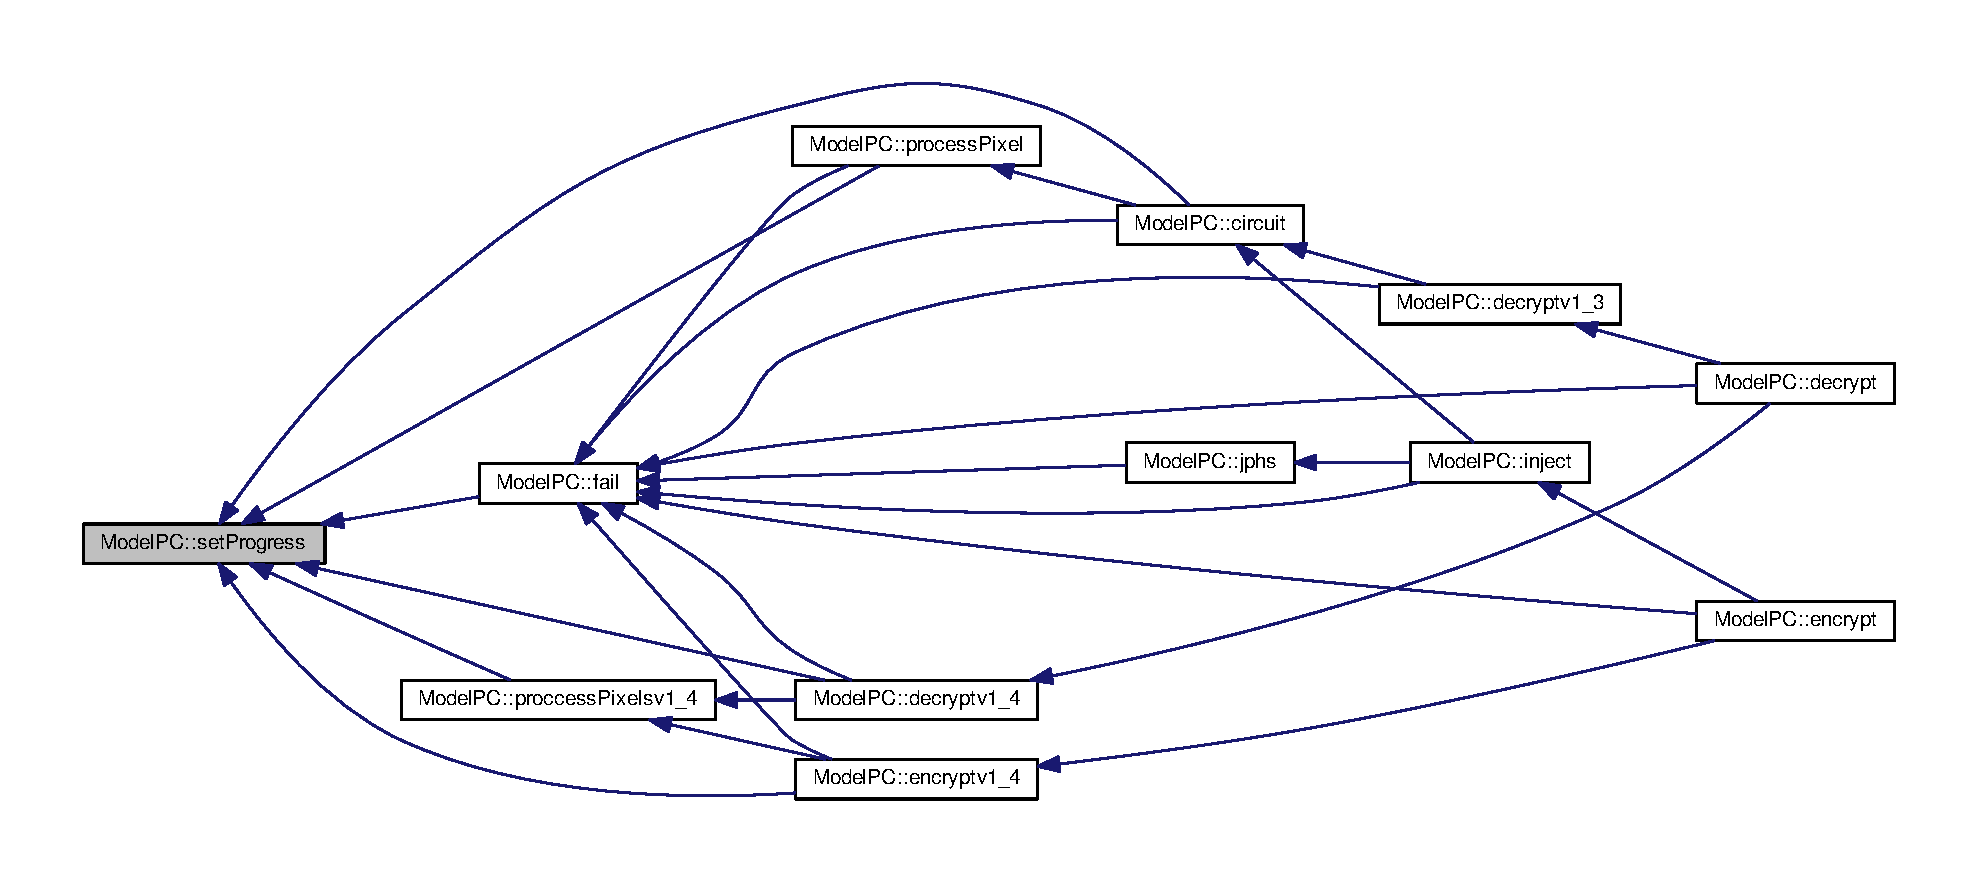
\includegraphics[width=350pt]{class_model_p_c_afdcd80f0ed5062e145a71f09b0897547_icgraph}
\end{center}
\end{figure}


\index{Model\+PC@{Model\+PC}!unzip@{unzip}}
\index{unzip@{unzip}!Model\+PC@{Model\+PC}}
\subsubsection[{\texorpdfstring{unzip(\+Q\+Byte\+Array data, Q\+Byte\+Array key)}{unzip(QByteArray data, QByteArray key)}}]{\setlength{\rightskip}{0pt plus 5cm}Q\+Byte\+Array Model\+P\+C\+::unzip (
\begin{DoxyParamCaption}
\item[{Q\+Byte\+Array}]{data, }
\item[{Q\+Byte\+Array}]{key}
\end{DoxyParamCaption}
)}\hypertarget{class_model_p_c_a6da88f166785a49f73b22c169f956fd0}{}\label{class_model_p_c_a6da88f166785a49f73b22c169f956fd0}


\hyperlink{class_model_p_c_a6da88f166785a49f73b22c169f956fd0}{Model\+P\+C\+::unzip} Unzip data from \hyperlink{class_model_p_c_a5995215a34a1e1f504035715a8013809}{Model\+P\+C\+::decrypt}. Just mirrored \hyperlink{class_encrypt_dialog_a2bff820a3df4ddc36ecb07ed74b7138a}{Encrypt\+Dialog\+::zip}. 


\begin{DoxyParams}{Parameters}
{\em data} & Data to be decrypted. \\
\hline
{\em key} & Key to decrypt the data. \\
\hline
\end{DoxyParams}
\begin{DoxyReturn}{Returns}
Returns data 
\end{DoxyReturn}
\begin{DoxySeeAlso}{See also}
\hyperlink{class_encrypt_dialog_a2bff820a3df4ddc36ecb07ed74b7138a}{Encrypt\+Dialog\+::zip}, \hyperlink{class_model_p_c_a5995215a34a1e1f504035715a8013809}{Model\+P\+C\+::decrypt}, \hyperlink{class_model_p_c_afebbbfa4b07deba4f68fc6dfb50f353f}{Model\+P\+C\+::zip} 
\end{DoxySeeAlso}


Definition at line \hyperlink{modelpc_8cpp_source_l00876}{876} of file \hyperlink{modelpc_8cpp_source}{modelpc.\+cpp}.



Here is the call graph for this function\+:
\nopagebreak
\begin{figure}[H]
\begin{center}
\leavevmode
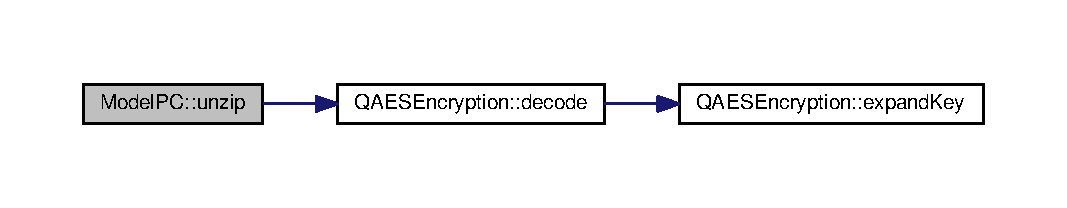
\includegraphics[width=350pt]{class_model_p_c_a6da88f166785a49f73b22c169f956fd0_cgraph}
\end{center}
\end{figure}




Here is the caller graph for this function\+:
\nopagebreak
\begin{figure}[H]
\begin{center}
\leavevmode
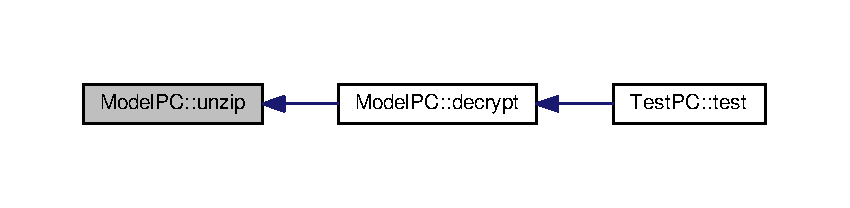
\includegraphics[width=350pt]{class_model_p_c_a6da88f166785a49f73b22c169f956fd0_icgraph}
\end{center}
\end{figure}


\index{Model\+PC@{Model\+PC}!zip@{zip}}
\index{zip@{zip}!Model\+PC@{Model\+PC}}
\subsubsection[{\texorpdfstring{zip(\+Q\+Byte\+Array data, Q\+Byte\+Array key)}{zip(QByteArray data, QByteArray key)}}]{\setlength{\rightskip}{0pt plus 5cm}Q\+Byte\+Array Model\+P\+C\+::zip (
\begin{DoxyParamCaption}
\item[{Q\+Byte\+Array}]{data, }
\item[{Q\+Byte\+Array}]{key}
\end{DoxyParamCaption}
)\hspace{0.3cm}{\ttfamily [protected]}}\hypertarget{class_model_p_c_afebbbfa4b07deba4f68fc6dfb50f353f}{}\label{class_model_p_c_afebbbfa4b07deba4f68fc6dfb50f353f}


\hyperlink{class_model_p_c_afebbbfa4b07deba4f68fc6dfb50f353f}{Model\+P\+C\+::zip} Zip function, copy of \hyperlink{class_encrypt_dialog_a2bff820a3df4ddc36ecb07ed74b7138a}{Encrypt\+Dialog\+::zip} Used for \hyperlink{class_model_p_c}{Model\+PC} in custom projects, other than Picture\+Crypt. 


\begin{DoxyParams}{Parameters}
{\em data} & Data to be encrypted \\
\hline
{\em key} & Key for encryption \\
\hline
\end{DoxyParams}
\begin{DoxyReturn}{Returns}
Returns decrypted data 
\end{DoxyReturn}
\begin{DoxySeeAlso}{See also}
Model\+P\+C\+::start, \hyperlink{class_model_p_c_aada6a04d81ada8f2b4ba18108c8d6f10}{Model\+P\+C\+::inject}, \hyperlink{class_model_p_c_a6da88f166785a49f73b22c169f956fd0}{Model\+P\+C\+::unzip} 
\end{DoxySeeAlso}


Definition at line \hyperlink{modelpc_8cpp_source_l00893}{893} of file \hyperlink{modelpc_8cpp_source}{modelpc.\+cpp}.



Here is the call graph for this function\+:
\nopagebreak
\begin{figure}[H]
\begin{center}
\leavevmode
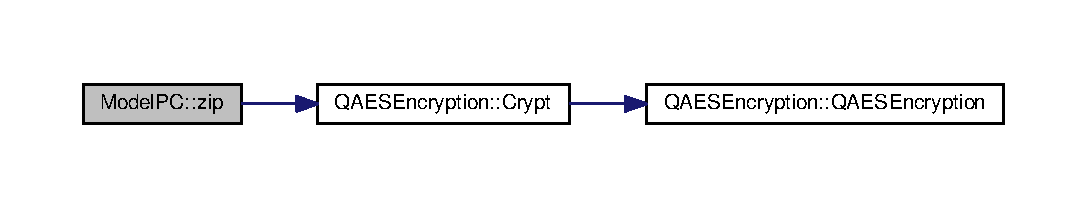
\includegraphics[width=350pt]{class_model_p_c_afebbbfa4b07deba4f68fc6dfb50f353f_cgraph}
\end{center}
\end{figure}




Here is the caller graph for this function\+:
\nopagebreak
\begin{figure}[H]
\begin{center}
\leavevmode
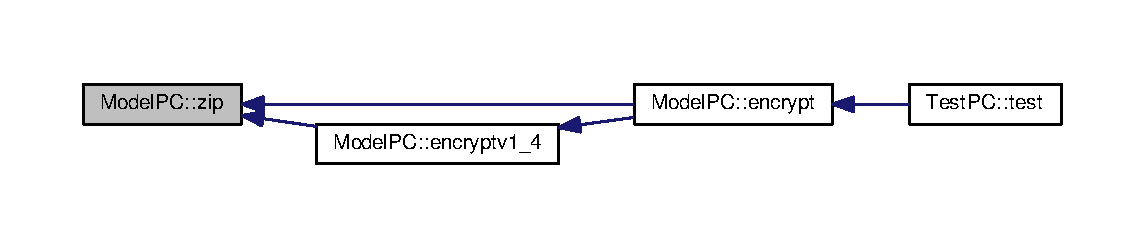
\includegraphics[width=350pt]{class_model_p_c_afebbbfa4b07deba4f68fc6dfb50f353f_icgraph}
\end{center}
\end{figure}




\subsection{Member Data Documentation}
\index{Model\+PC@{Model\+PC}!default\+J\+P\+H\+S\+Dir@{default\+J\+P\+H\+S\+Dir}}
\index{default\+J\+P\+H\+S\+Dir@{default\+J\+P\+H\+S\+Dir}!Model\+PC@{Model\+PC}}
\subsubsection[{\texorpdfstring{default\+J\+P\+H\+S\+Dir}{defaultJPHSDir}}]{\setlength{\rightskip}{0pt plus 5cm}Q\+String Model\+P\+C\+::default\+J\+P\+H\+S\+Dir}\hypertarget{class_model_p_c_abd038306f14f22fb885a1697c96d6335}{}\label{class_model_p_c_abd038306f14f22fb885a1697c96d6335}


default\+J\+P\+H\+S\+Dir Default J\+P\+HS directory 



Definition at line \hyperlink{modelpc_8h_source_l00094}{94} of file \hyperlink{modelpc_8h_source}{modelpc.\+h}.

\index{Model\+PC@{Model\+PC}!error@{error}}
\index{error@{error}!Model\+PC@{Model\+PC}}
\subsubsection[{\texorpdfstring{error}{error}}]{\setlength{\rightskip}{0pt plus 5cm}Q\+String$\ast$ Model\+P\+C\+::error\hspace{0.3cm}{\ttfamily [protected]}}\hypertarget{class_model_p_c_a4e5a9c0ca1f06fe5bc478b6bf248c37c}{}\label{class_model_p_c_a4e5a9c0ca1f06fe5bc478b6bf248c37c}


error Current error 



Definition at line \hyperlink{modelpc_8h_source_l00108}{108} of file \hyperlink{modelpc_8h_source}{modelpc.\+h}.

\index{Model\+PC@{Model\+PC}!success@{success}}
\index{success@{success}!Model\+PC@{Model\+PC}}
\subsubsection[{\texorpdfstring{success}{success}}]{\setlength{\rightskip}{0pt plus 5cm}bool Model\+P\+C\+::success}\hypertarget{class_model_p_c_a945ffbbc44a832b953c191debd448f4c}{}\label{class_model_p_c_a945ffbbc44a832b953c191debd448f4c}


success Flag that true by default, but in case of error or cancelling of Progress\+Dialog it turns to false, which stops execution of \hyperlink{class_model_p_c_a1d0091062a0c836b283ec2f67411623b}{Model\+P\+C\+::circuit} 



Definition at line \hyperlink{modelpc_8h_source_l00082}{82} of file \hyperlink{modelpc_8h_source}{modelpc.\+h}.

\index{Model\+PC@{Model\+PC}!version@{version}}
\index{version@{version}!Model\+PC@{Model\+PC}}
\subsubsection[{\texorpdfstring{version}{version}}]{\setlength{\rightskip}{0pt plus 5cm}long Model\+P\+C\+::version}\hypertarget{class_model_p_c_a5af48ab89e19be42a94c34ba00249401}{}\label{class_model_p_c_a5af48ab89e19be42a94c34ba00249401}


version Version of the class 



Definition at line \hyperlink{modelpc_8h_source_l00086}{86} of file \hyperlink{modelpc_8h_source}{modelpc.\+h}.

\index{Model\+PC@{Model\+PC}!version\+String@{version\+String}}
\index{version\+String@{version\+String}!Model\+PC@{Model\+PC}}
\subsubsection[{\texorpdfstring{version\+String}{versionString}}]{\setlength{\rightskip}{0pt plus 5cm}Q\+String Model\+P\+C\+::version\+String}\hypertarget{class_model_p_c_a5f426725ccf7eefd3c77ea8c720264c9}{}\label{class_model_p_c_a5f426725ccf7eefd3c77ea8c720264c9}


version\+String Version as string 



Definition at line \hyperlink{modelpc_8h_source_l00090}{90} of file \hyperlink{modelpc_8h_source}{modelpc.\+h}.



The documentation for this class was generated from the following files\+:\begin{DoxyCompactItemize}
\item 
\hyperlink{modelpc_8h}{modelpc.\+h}\item 
\hyperlink{modelpc_8cpp}{modelpc.\+cpp}\end{DoxyCompactItemize}

\hypertarget{class_q_a_e_s_encryption}{\section{Q\-A\-E\-S\-Encryption Class Reference}
\label{class_q_a_e_s_encryption}\index{Q\-A\-E\-S\-Encryption@{Q\-A\-E\-S\-Encryption}}
}


The \hyperlink{class_q_a_e_s_encryption}{Q\-A\-E\-S\-Encryption} class Small and portable A\-E\-S encryption class for Qt. Supports all key sizes -\/ 128/192/256 bits -\/ E\-C\-B, C\-B\-C, C\-F\-B and O\-F\-B modes. Class made entirely by bricke. Github\-: \href{https://github.com/bricke/Qt-AES}{\tt https\-://github.\-com/bricke/\-Qt-\/\-A\-E\-S}.  




{\ttfamily \#include $<$qaesencryption.\-h$>$}



Inheritance diagram for Q\-A\-E\-S\-Encryption\-:
\nopagebreak
\begin{figure}[H]
\begin{center}
\leavevmode
\includegraphics[width=170pt]{class_q_a_e_s_encryption__inherit__graph}
\end{center}
\end{figure}


Collaboration diagram for Q\-A\-E\-S\-Encryption\-:
\nopagebreak
\begin{figure}[H]
\begin{center}
\leavevmode
\includegraphics[width=170pt]{class_q_a_e_s_encryption__coll__graph}
\end{center}
\end{figure}
\subsection*{Public Types}
\begin{DoxyCompactItemize}
\item 
enum \hyperlink{class_q_a_e_s_encryption_abe48208f4f6c7d68e6a10b49b9d0b7bd}{Aes} \{ \hyperlink{class_q_a_e_s_encryption_abe48208f4f6c7d68e6a10b49b9d0b7bda0fa01cdf69e5537499ecfc6f96d6570a}{A\-E\-S\-\_\-128}, 
\hyperlink{class_q_a_e_s_encryption_abe48208f4f6c7d68e6a10b49b9d0b7bda7bd082b240582de6d5f4b8ea604e646b}{A\-E\-S\-\_\-192}, 
\hyperlink{class_q_a_e_s_encryption_abe48208f4f6c7d68e6a10b49b9d0b7bdacde97774ab1d4c609e04b0dd13a1e1f7}{A\-E\-S\-\_\-256}
 \}
\begin{DoxyCompactList}\small\item\em The Aes enum A\-E\-S Level A\-E\-S Levels The class supports all A\-E\-S key lenghts. \end{DoxyCompactList}\item 
enum \hyperlink{class_q_a_e_s_encryption_ad3e031c49a3d56566379d75b40b7b255}{Mode} \{ \hyperlink{class_q_a_e_s_encryption_ad3e031c49a3d56566379d75b40b7b255a4ca7f51778e2adf1f464164a0ba8e75e}{E\-C\-B}, 
\hyperlink{class_q_a_e_s_encryption_ad3e031c49a3d56566379d75b40b7b255a559bffc55d3599d0a172cc85aed98966}{C\-B\-C}, 
\hyperlink{class_q_a_e_s_encryption_ad3e031c49a3d56566379d75b40b7b255ae5e2e019df35c7d172fcd7f0ebec5e8e}{C\-F\-B}, 
\hyperlink{class_q_a_e_s_encryption_ad3e031c49a3d56566379d75b40b7b255a27e2f82decd94080893d61db4a8adcb3}{O\-F\-B}
 \}
\begin{DoxyCompactList}\small\item\em The Mode enum A\-E\-S Mode The class supports the following operating modes E\-C\-B C\-B\-C C\-F\-B O\-F\-B. \end{DoxyCompactList}\item 
enum \hyperlink{class_q_a_e_s_encryption_ab0a65cdea4eac21ef32530010d1b0247}{Padding} \{ \hyperlink{class_q_a_e_s_encryption_ab0a65cdea4eac21ef32530010d1b0247a0842d5191caeff6f871908fa7b9e8e7a}{Z\-E\-R\-O}, 
\hyperlink{class_q_a_e_s_encryption_ab0a65cdea4eac21ef32530010d1b0247a74a898410a12cbc5391b47daa04cbd69}{P\-K\-C\-S7}, 
\hyperlink{class_q_a_e_s_encryption_ab0a65cdea4eac21ef32530010d1b0247a4fb686e6a16d4242ff35311d2e7c422d}{I\-S\-O}
 \}
\begin{DoxyCompactList}\small\item\em The Padding enum Padding By default the padding method is I\-S\-O, however, the class supports\-: \end{DoxyCompactList}\end{DoxyCompactItemize}
\subsection*{Public Member Functions}
\begin{DoxyCompactItemize}
\item 
\hyperlink{class_q_a_e_s_encryption_aeac0ee8532e69e5d30b023fe38c30b3b}{Q\-A\-E\-S\-Encryption} (\hyperlink{class_q_a_e_s_encryption_abe48208f4f6c7d68e6a10b49b9d0b7bd}{Q\-A\-E\-S\-Encryption\-::\-Aes} level, \hyperlink{class_q_a_e_s_encryption_ad3e031c49a3d56566379d75b40b7b255}{Q\-A\-E\-S\-Encryption\-::\-Mode} mode, \hyperlink{class_q_a_e_s_encryption_ab0a65cdea4eac21ef32530010d1b0247}{Q\-A\-E\-S\-Encryption\-::\-Padding} padding=\hyperlink{class_q_a_e_s_encryption_ab0a65cdea4eac21ef32530010d1b0247a4fb686e6a16d4242ff35311d2e7c422d}{Q\-A\-E\-S\-Encryption\-::\-I\-S\-O})
\item 
Q\-Byte\-Array \hyperlink{class_q_a_e_s_encryption_a0c56eddd6f03e93b1f7faad464044d65}{encode} (const Q\-Byte\-Array \&raw\-Text, const Q\-Byte\-Array \&key, const Q\-Byte\-Array \&iv=N\-U\-L\-L)
\begin{DoxyCompactList}\small\item\em encode Encodes data with A\-E\-S \end{DoxyCompactList}\item 
Q\-Byte\-Array \hyperlink{class_q_a_e_s_encryption_a58f972f2b66c2454edd5112495463bba}{decode} (const Q\-Byte\-Array \&raw\-Text, const Q\-Byte\-Array \&key, const Q\-Byte\-Array \&iv=N\-U\-L\-L)
\begin{DoxyCompactList}\small\item\em decode Decodes data with A\-E\-S \end{DoxyCompactList}\item 
Q\-Byte\-Array \hyperlink{class_q_a_e_s_encryption_a4dc7e77485e5a3e63eebc99b9386c17b}{remove\-Padding} (const Q\-Byte\-Array \&raw\-Text)
\begin{DoxyCompactList}\small\item\em Remove\-Padding Removes padding. \end{DoxyCompactList}\item 
Q\-Byte\-Array \hyperlink{class_q_a_e_s_encryption_a5bfbb972f84a8376fceed648553c0912}{expand\-Key} (const Q\-Byte\-Array \&key)
\begin{DoxyCompactList}\small\item\em Expand\-Key Expands the key. \end{DoxyCompactList}\end{DoxyCompactItemize}
\subsection*{Static Public Member Functions}
\begin{DoxyCompactItemize}
\item 
static Q\-Byte\-Array \hyperlink{class_q_a_e_s_encryption_a43819eeb6a7cb29fbd3cb6ad640dcbdf}{Crypt} (\hyperlink{class_q_a_e_s_encryption_abe48208f4f6c7d68e6a10b49b9d0b7bd}{Q\-A\-E\-S\-Encryption\-::\-Aes} level, \hyperlink{class_q_a_e_s_encryption_ad3e031c49a3d56566379d75b40b7b255}{Q\-A\-E\-S\-Encryption\-::\-Mode} mode, const Q\-Byte\-Array \&raw\-Text, const Q\-Byte\-Array \&key, const Q\-Byte\-Array \&iv=N\-U\-L\-L, \hyperlink{class_q_a_e_s_encryption_ab0a65cdea4eac21ef32530010d1b0247}{Q\-A\-E\-S\-Encryption\-::\-Padding} padding=\hyperlink{class_q_a_e_s_encryption_ab0a65cdea4eac21ef32530010d1b0247a4fb686e6a16d4242ff35311d2e7c422d}{Q\-A\-E\-S\-Encryption\-::\-I\-S\-O})
\begin{DoxyCompactList}\small\item\em Crypt Static encode function. \end{DoxyCompactList}\item 
static Q\-Byte\-Array \hyperlink{class_q_a_e_s_encryption_af9baa154a06683049d941bd06ac698fd}{Decrypt} (\hyperlink{class_q_a_e_s_encryption_abe48208f4f6c7d68e6a10b49b9d0b7bd}{Q\-A\-E\-S\-Encryption\-::\-Aes} level, \hyperlink{class_q_a_e_s_encryption_ad3e031c49a3d56566379d75b40b7b255}{Q\-A\-E\-S\-Encryption\-::\-Mode} mode, const Q\-Byte\-Array \&raw\-Text, const Q\-Byte\-Array \&key, const Q\-Byte\-Array \&iv=N\-U\-L\-L, \hyperlink{class_q_a_e_s_encryption_ab0a65cdea4eac21ef32530010d1b0247}{Q\-A\-E\-S\-Encryption\-::\-Padding} padding=\hyperlink{class_q_a_e_s_encryption_ab0a65cdea4eac21ef32530010d1b0247a4fb686e6a16d4242ff35311d2e7c422d}{Q\-A\-E\-S\-Encryption\-::\-I\-S\-O})
\begin{DoxyCompactList}\small\item\em Decrypt Static decode function. \end{DoxyCompactList}\item 
static Q\-Byte\-Array \hyperlink{class_q_a_e_s_encryption_a2112456e057e6dd886694348fbf202cd}{Expand\-Key} (\hyperlink{class_q_a_e_s_encryption_abe48208f4f6c7d68e6a10b49b9d0b7bd}{Q\-A\-E\-S\-Encryption\-::\-Aes} level, \hyperlink{class_q_a_e_s_encryption_ad3e031c49a3d56566379d75b40b7b255}{Q\-A\-E\-S\-Encryption\-::\-Mode} mode, const Q\-Byte\-Array \&key)
\begin{DoxyCompactList}\small\item\em Expand\-Key Expands the key. \end{DoxyCompactList}\item 
static Q\-Byte\-Array \hyperlink{class_q_a_e_s_encryption_abb2887bf5623a74053dd19627f3d3055}{Remove\-Padding} (const Q\-Byte\-Array \&raw\-Text, \hyperlink{class_q_a_e_s_encryption_ab0a65cdea4eac21ef32530010d1b0247}{Q\-A\-E\-S\-Encryption\-::\-Padding} padding)
\begin{DoxyCompactList}\small\item\em Remove\-Padding Removes padding. \end{DoxyCompactList}\end{DoxyCompactItemize}


\subsection{Detailed Description}
The \hyperlink{class_q_a_e_s_encryption}{Q\-A\-E\-S\-Encryption} class Small and portable A\-E\-S encryption class for Qt. Supports all key sizes -\/ 128/192/256 bits -\/ E\-C\-B, C\-B\-C, C\-F\-B and O\-F\-B modes. Class made entirely by bricke. Github\-: \href{https://github.com/bricke/Qt-AES}{\tt https\-://github.\-com/bricke/\-Qt-\/\-A\-E\-S}. 

\begin{DoxyAuthor}{Author}
Bricke (Matteo B) 
\end{DoxyAuthor}


Definition at line \hyperlink{qaesencryption_8h_source_l00014}{14} of file \hyperlink{qaesencryption_8h_source}{qaesencryption.\-h}.



\subsection{Member Enumeration Documentation}
\hypertarget{class_q_a_e_s_encryption_abe48208f4f6c7d68e6a10b49b9d0b7bd}{\index{Q\-A\-E\-S\-Encryption@{Q\-A\-E\-S\-Encryption}!Aes@{Aes}}
\index{Aes@{Aes}!QAESEncryption@{Q\-A\-E\-S\-Encryption}}
\subsubsection[{Aes}]{\setlength{\rightskip}{0pt plus 5cm}enum {\bf Q\-A\-E\-S\-Encryption\-::\-Aes}}}\label{class_q_a_e_s_encryption_abe48208f4f6c7d68e6a10b49b9d0b7bd}


The Aes enum A\-E\-S Level A\-E\-S Levels The class supports all A\-E\-S key lenghts. 

A\-E\-S\-\_\-128 A\-E\-S\-\_\-192 A\-E\-S\-\_\-256 \begin{Desc}
\item[Enumerator]\par
\begin{description}
\index{A\-E\-S\-\_\-128@{A\-E\-S\-\_\-128}!Q\-A\-E\-S\-Encryption@{Q\-A\-E\-S\-Encryption}}\index{Q\-A\-E\-S\-Encryption@{Q\-A\-E\-S\-Encryption}!A\-E\-S\-\_\-128@{A\-E\-S\-\_\-128}}\item[{\em 
\hypertarget{class_q_a_e_s_encryption_abe48208f4f6c7d68e6a10b49b9d0b7bda0fa01cdf69e5537499ecfc6f96d6570a}{A\-E\-S\-\_\-128}\label{class_q_a_e_s_encryption_abe48208f4f6c7d68e6a10b49b9d0b7bda0fa01cdf69e5537499ecfc6f96d6570a}
}]\index{A\-E\-S\-\_\-192@{A\-E\-S\-\_\-192}!Q\-A\-E\-S\-Encryption@{Q\-A\-E\-S\-Encryption}}\index{Q\-A\-E\-S\-Encryption@{Q\-A\-E\-S\-Encryption}!A\-E\-S\-\_\-192@{A\-E\-S\-\_\-192}}\item[{\em 
\hypertarget{class_q_a_e_s_encryption_abe48208f4f6c7d68e6a10b49b9d0b7bda7bd082b240582de6d5f4b8ea604e646b}{A\-E\-S\-\_\-192}\label{class_q_a_e_s_encryption_abe48208f4f6c7d68e6a10b49b9d0b7bda7bd082b240582de6d5f4b8ea604e646b}
}]\index{A\-E\-S\-\_\-256@{A\-E\-S\-\_\-256}!Q\-A\-E\-S\-Encryption@{Q\-A\-E\-S\-Encryption}}\index{Q\-A\-E\-S\-Encryption@{Q\-A\-E\-S\-Encryption}!A\-E\-S\-\_\-256@{A\-E\-S\-\_\-256}}\item[{\em 
\hypertarget{class_q_a_e_s_encryption_abe48208f4f6c7d68e6a10b49b9d0b7bdacde97774ab1d4c609e04b0dd13a1e1f7}{A\-E\-S\-\_\-256}\label{class_q_a_e_s_encryption_abe48208f4f6c7d68e6a10b49b9d0b7bdacde97774ab1d4c609e04b0dd13a1e1f7}
}]\end{description}
\end{Desc}


Definition at line \hyperlink{qaesencryption_8h_source_l00027}{27} of file \hyperlink{qaesencryption_8h_source}{qaesencryption.\-h}.

\hypertarget{class_q_a_e_s_encryption_ad3e031c49a3d56566379d75b40b7b255}{\index{Q\-A\-E\-S\-Encryption@{Q\-A\-E\-S\-Encryption}!Mode@{Mode}}
\index{Mode@{Mode}!QAESEncryption@{Q\-A\-E\-S\-Encryption}}
\subsubsection[{Mode}]{\setlength{\rightskip}{0pt plus 5cm}enum {\bf Q\-A\-E\-S\-Encryption\-::\-Mode}}}\label{class_q_a_e_s_encryption_ad3e031c49a3d56566379d75b40b7b255}


The Mode enum A\-E\-S Mode The class supports the following operating modes E\-C\-B C\-B\-C C\-F\-B O\-F\-B. 

\begin{Desc}
\item[Enumerator]\par
\begin{description}
\index{E\-C\-B@{E\-C\-B}!Q\-A\-E\-S\-Encryption@{Q\-A\-E\-S\-Encryption}}\index{Q\-A\-E\-S\-Encryption@{Q\-A\-E\-S\-Encryption}!E\-C\-B@{E\-C\-B}}\item[{\em 
\hypertarget{class_q_a_e_s_encryption_ad3e031c49a3d56566379d75b40b7b255a4ca7f51778e2adf1f464164a0ba8e75e}{E\-C\-B}\label{class_q_a_e_s_encryption_ad3e031c49a3d56566379d75b40b7b255a4ca7f51778e2adf1f464164a0ba8e75e}
}]\index{C\-B\-C@{C\-B\-C}!Q\-A\-E\-S\-Encryption@{Q\-A\-E\-S\-Encryption}}\index{Q\-A\-E\-S\-Encryption@{Q\-A\-E\-S\-Encryption}!C\-B\-C@{C\-B\-C}}\item[{\em 
\hypertarget{class_q_a_e_s_encryption_ad3e031c49a3d56566379d75b40b7b255a559bffc55d3599d0a172cc85aed98966}{C\-B\-C}\label{class_q_a_e_s_encryption_ad3e031c49a3d56566379d75b40b7b255a559bffc55d3599d0a172cc85aed98966}
}]\index{C\-F\-B@{C\-F\-B}!Q\-A\-E\-S\-Encryption@{Q\-A\-E\-S\-Encryption}}\index{Q\-A\-E\-S\-Encryption@{Q\-A\-E\-S\-Encryption}!C\-F\-B@{C\-F\-B}}\item[{\em 
\hypertarget{class_q_a_e_s_encryption_ad3e031c49a3d56566379d75b40b7b255ae5e2e019df35c7d172fcd7f0ebec5e8e}{C\-F\-B}\label{class_q_a_e_s_encryption_ad3e031c49a3d56566379d75b40b7b255ae5e2e019df35c7d172fcd7f0ebec5e8e}
}]\index{O\-F\-B@{O\-F\-B}!Q\-A\-E\-S\-Encryption@{Q\-A\-E\-S\-Encryption}}\index{Q\-A\-E\-S\-Encryption@{Q\-A\-E\-S\-Encryption}!O\-F\-B@{O\-F\-B}}\item[{\em 
\hypertarget{class_q_a_e_s_encryption_ad3e031c49a3d56566379d75b40b7b255a27e2f82decd94080893d61db4a8adcb3}{O\-F\-B}\label{class_q_a_e_s_encryption_ad3e031c49a3d56566379d75b40b7b255a27e2f82decd94080893d61db4a8adcb3}
}]\end{description}
\end{Desc}


Definition at line \hyperlink{qaesencryption_8h_source_l00040}{40} of file \hyperlink{qaesencryption_8h_source}{qaesencryption.\-h}.

\hypertarget{class_q_a_e_s_encryption_ab0a65cdea4eac21ef32530010d1b0247}{\index{Q\-A\-E\-S\-Encryption@{Q\-A\-E\-S\-Encryption}!Padding@{Padding}}
\index{Padding@{Padding}!QAESEncryption@{Q\-A\-E\-S\-Encryption}}
\subsubsection[{Padding}]{\setlength{\rightskip}{0pt plus 5cm}enum {\bf Q\-A\-E\-S\-Encryption\-::\-Padding}}}\label{class_q_a_e_s_encryption_ab0a65cdea4eac21ef32530010d1b0247}


The Padding enum Padding By default the padding method is I\-S\-O, however, the class supports\-: 

Z\-E\-R\-O P\-K\-C\-S7 I\-S\-O \begin{Desc}
\item[Enumerator]\par
\begin{description}
\index{Z\-E\-R\-O@{Z\-E\-R\-O}!Q\-A\-E\-S\-Encryption@{Q\-A\-E\-S\-Encryption}}\index{Q\-A\-E\-S\-Encryption@{Q\-A\-E\-S\-Encryption}!Z\-E\-R\-O@{Z\-E\-R\-O}}\item[{\em 
\hypertarget{class_q_a_e_s_encryption_ab0a65cdea4eac21ef32530010d1b0247a0842d5191caeff6f871908fa7b9e8e7a}{Z\-E\-R\-O}\label{class_q_a_e_s_encryption_ab0a65cdea4eac21ef32530010d1b0247a0842d5191caeff6f871908fa7b9e8e7a}
}]\index{P\-K\-C\-S7@{P\-K\-C\-S7}!Q\-A\-E\-S\-Encryption@{Q\-A\-E\-S\-Encryption}}\index{Q\-A\-E\-S\-Encryption@{Q\-A\-E\-S\-Encryption}!P\-K\-C\-S7@{P\-K\-C\-S7}}\item[{\em 
\hypertarget{class_q_a_e_s_encryption_ab0a65cdea4eac21ef32530010d1b0247a74a898410a12cbc5391b47daa04cbd69}{P\-K\-C\-S7}\label{class_q_a_e_s_encryption_ab0a65cdea4eac21ef32530010d1b0247a74a898410a12cbc5391b47daa04cbd69}
}]\index{I\-S\-O@{I\-S\-O}!Q\-A\-E\-S\-Encryption@{Q\-A\-E\-S\-Encryption}}\index{Q\-A\-E\-S\-Encryption@{Q\-A\-E\-S\-Encryption}!I\-S\-O@{I\-S\-O}}\item[{\em 
\hypertarget{class_q_a_e_s_encryption_ab0a65cdea4eac21ef32530010d1b0247a4fb686e6a16d4242ff35311d2e7c422d}{I\-S\-O}\label{class_q_a_e_s_encryption_ab0a65cdea4eac21ef32530010d1b0247a4fb686e6a16d4242ff35311d2e7c422d}
}]\end{description}
\end{Desc}


Definition at line \hyperlink{qaesencryption_8h_source_l00055}{55} of file \hyperlink{qaesencryption_8h_source}{qaesencryption.\-h}.



\subsection{Constructor \& Destructor Documentation}
\hypertarget{class_q_a_e_s_encryption_aeac0ee8532e69e5d30b023fe38c30b3b}{\index{Q\-A\-E\-S\-Encryption@{Q\-A\-E\-S\-Encryption}!Q\-A\-E\-S\-Encryption@{Q\-A\-E\-S\-Encryption}}
\index{Q\-A\-E\-S\-Encryption@{Q\-A\-E\-S\-Encryption}!QAESEncryption@{Q\-A\-E\-S\-Encryption}}
\subsubsection[{Q\-A\-E\-S\-Encryption}]{\setlength{\rightskip}{0pt plus 5cm}Q\-A\-E\-S\-Encryption\-::\-Q\-A\-E\-S\-Encryption (
\begin{DoxyParamCaption}
\item[{{\bf Q\-A\-E\-S\-Encryption\-::\-Aes}}]{level, }
\item[{{\bf Q\-A\-E\-S\-Encryption\-::\-Mode}}]{mode, }
\item[{{\bf Q\-A\-E\-S\-Encryption\-::\-Padding}}]{padding = {\ttfamily {\bf Q\-A\-E\-S\-Encryption\-::\-I\-S\-O}}}
\end{DoxyParamCaption}
)}}\label{class_q_a_e_s_encryption_aeac0ee8532e69e5d30b023fe38c30b3b}


Definition at line \hyperlink{qaesencryption_8cpp_source_l00067}{67} of file \hyperlink{qaesencryption_8cpp_source}{qaesencryption.\-cpp}.



Here is the caller graph for this function\-:
\nopagebreak
\begin{figure}[H]
\begin{center}
\leavevmode
\includegraphics[width=350pt]{class_q_a_e_s_encryption_aeac0ee8532e69e5d30b023fe38c30b3b_icgraph}
\end{center}
\end{figure}




\subsection{Member Function Documentation}
\hypertarget{class_q_a_e_s_encryption_a43819eeb6a7cb29fbd3cb6ad640dcbdf}{\index{Q\-A\-E\-S\-Encryption@{Q\-A\-E\-S\-Encryption}!Crypt@{Crypt}}
\index{Crypt@{Crypt}!QAESEncryption@{Q\-A\-E\-S\-Encryption}}
\subsubsection[{Crypt}]{\setlength{\rightskip}{0pt plus 5cm}Q\-Byte\-Array Q\-A\-E\-S\-Encryption\-::\-Crypt (
\begin{DoxyParamCaption}
\item[{{\bf Q\-A\-E\-S\-Encryption\-::\-Aes}}]{level, }
\item[{{\bf Q\-A\-E\-S\-Encryption\-::\-Mode}}]{mode, }
\item[{const Q\-Byte\-Array \&}]{raw\-Text, }
\item[{const Q\-Byte\-Array \&}]{key, }
\item[{const Q\-Byte\-Array \&}]{iv = {\ttfamily NULL}, }
\item[{{\bf Q\-A\-E\-S\-Encryption\-::\-Padding}}]{padding = {\ttfamily {\bf Q\-A\-E\-S\-Encryption\-::\-I\-S\-O}}}
\end{DoxyParamCaption}
)\hspace{0.3cm}{\ttfamily [static]}}}\label{class_q_a_e_s_encryption_a43819eeb6a7cb29fbd3cb6ad640dcbdf}


Crypt Static encode function. 


\begin{DoxyParams}{Parameters}
{\em level} & A\-E\-S level of encryption \\
\hline
{\em mode} & A\-E\-S mode \\
\hline
{\em raw\-Text} & Input data \\
\hline
{\em key} & Key for encrytion \\
\hline
{\em iv} & I\-V vector \\
\hline
{\em padding} & Padding \\
\hline
\end{DoxyParams}
\begin{DoxyReturn}{Returns}
Returns encrypted data 
\end{DoxyReturn}
\begin{DoxySeeAlso}{See Also}
\hyperlink{class_q_a_e_s_encryption_a0c56eddd6f03e93b1f7faad464044d65}{Q\-A\-E\-S\-Encryption\-::encode}, \hyperlink{class_q_a_e_s_encryption_af9baa154a06683049d941bd06ac698fd}{Q\-A\-E\-S\-Encryption\-::\-Decrypt} 
\end{DoxySeeAlso}


Definition at line \hyperlink{qaesencryption_8cpp_source_l00006}{6} of file \hyperlink{qaesencryption_8cpp_source}{qaesencryption.\-cpp}.



Here is the call graph for this function\-:
\nopagebreak
\begin{figure}[H]
\begin{center}
\leavevmode
\includegraphics[width=350pt]{class_q_a_e_s_encryption_a43819eeb6a7cb29fbd3cb6ad640dcbdf_cgraph}
\end{center}
\end{figure}




Here is the caller graph for this function\-:
\nopagebreak
\begin{figure}[H]
\begin{center}
\leavevmode
\includegraphics[width=350pt]{class_q_a_e_s_encryption_a43819eeb6a7cb29fbd3cb6ad640dcbdf_icgraph}
\end{center}
\end{figure}


\hypertarget{class_q_a_e_s_encryption_a58f972f2b66c2454edd5112495463bba}{\index{Q\-A\-E\-S\-Encryption@{Q\-A\-E\-S\-Encryption}!decode@{decode}}
\index{decode@{decode}!QAESEncryption@{Q\-A\-E\-S\-Encryption}}
\subsubsection[{decode}]{\setlength{\rightskip}{0pt plus 5cm}Q\-Byte\-Array Q\-A\-E\-S\-Encryption\-::decode (
\begin{DoxyParamCaption}
\item[{const Q\-Byte\-Array \&}]{raw\-Text, }
\item[{const Q\-Byte\-Array \&}]{key, }
\item[{const Q\-Byte\-Array \&}]{iv = {\ttfamily NULL}}
\end{DoxyParamCaption}
)}}\label{class_q_a_e_s_encryption_a58f972f2b66c2454edd5112495463bba}


decode Decodes data with A\-E\-S 

\begin{DoxyNote}{Note}
Basically the non-\/static method of \hyperlink{class_q_a_e_s_encryption_af9baa154a06683049d941bd06ac698fd}{Q\-A\-E\-S\-Encryption\-::\-Decrypt}
\end{DoxyNote}

\begin{DoxyParams}{Parameters}
{\em raw\-Text} & Input data \\
\hline
{\em key} & Key \\
\hline
{\em iv} & I\-V vector \\
\hline
\end{DoxyParams}
\begin{DoxyReturn}{Returns}
Returns decoded data 
\end{DoxyReturn}
\begin{DoxySeeAlso}{See Also}
\hyperlink{class_q_a_e_s_encryption_af9baa154a06683049d941bd06ac698fd}{Q\-A\-E\-S\-Encryption\-::\-Decrypt}, \hyperlink{class_q_a_e_s_encryption_a0c56eddd6f03e93b1f7faad464044d65}{Q\-A\-E\-S\-Encryption\-::encode} 
\end{DoxySeeAlso}


Definition at line \hyperlink{qaesencryption_8cpp_source_l00441}{441} of file \hyperlink{qaesencryption_8cpp_source}{qaesencryption.\-cpp}.



Here is the call graph for this function\-:
\nopagebreak
\begin{figure}[H]
\begin{center}
\leavevmode
\includegraphics[width=350pt]{class_q_a_e_s_encryption_a58f972f2b66c2454edd5112495463bba_cgraph}
\end{center}
\end{figure}




Here is the caller graph for this function\-:
\nopagebreak
\begin{figure}[H]
\begin{center}
\leavevmode
\includegraphics[width=350pt]{class_q_a_e_s_encryption_a58f972f2b66c2454edd5112495463bba_icgraph}
\end{center}
\end{figure}


\hypertarget{class_q_a_e_s_encryption_af9baa154a06683049d941bd06ac698fd}{\index{Q\-A\-E\-S\-Encryption@{Q\-A\-E\-S\-Encryption}!Decrypt@{Decrypt}}
\index{Decrypt@{Decrypt}!QAESEncryption@{Q\-A\-E\-S\-Encryption}}
\subsubsection[{Decrypt}]{\setlength{\rightskip}{0pt plus 5cm}Q\-Byte\-Array Q\-A\-E\-S\-Encryption\-::\-Decrypt (
\begin{DoxyParamCaption}
\item[{{\bf Q\-A\-E\-S\-Encryption\-::\-Aes}}]{level, }
\item[{{\bf Q\-A\-E\-S\-Encryption\-::\-Mode}}]{mode, }
\item[{const Q\-Byte\-Array \&}]{raw\-Text, }
\item[{const Q\-Byte\-Array \&}]{key, }
\item[{const Q\-Byte\-Array \&}]{iv = {\ttfamily NULL}, }
\item[{{\bf Q\-A\-E\-S\-Encryption\-::\-Padding}}]{padding = {\ttfamily {\bf Q\-A\-E\-S\-Encryption\-::\-I\-S\-O}}}
\end{DoxyParamCaption}
)\hspace{0.3cm}{\ttfamily [static]}}}\label{class_q_a_e_s_encryption_af9baa154a06683049d941bd06ac698fd}


Decrypt Static decode function. 


\begin{DoxyParams}{Parameters}
{\em level} & A\-E\-S level of encryption \\
\hline
{\em mode} & A\-E\-S mode \\
\hline
{\em raw\-Text} & Encrypted data \\
\hline
{\em key} & Key for encrytion \\
\hline
{\em iv} & I\-V vector \\
\hline
{\em padding} & Padding \\
\hline
\end{DoxyParams}
\begin{DoxyReturn}{Returns}
Returns Decrypted data 
\end{DoxyReturn}
\begin{DoxySeeAlso}{See Also}
\hyperlink{class_q_a_e_s_encryption_a58f972f2b66c2454edd5112495463bba}{Q\-A\-E\-S\-Encryption\-::decode}, \hyperlink{class_q_a_e_s_encryption_a43819eeb6a7cb29fbd3cb6ad640dcbdf}{Q\-A\-E\-S\-Encryption\-::\-Crypt} 
\end{DoxySeeAlso}


Definition at line \hyperlink{qaesencryption_8cpp_source_l00012}{12} of file \hyperlink{qaesencryption_8cpp_source}{qaesencryption.\-cpp}.



Here is the call graph for this function\-:
\nopagebreak
\begin{figure}[H]
\begin{center}
\leavevmode
\includegraphics[width=350pt]{class_q_a_e_s_encryption_af9baa154a06683049d941bd06ac698fd_cgraph}
\end{center}
\end{figure}


\hypertarget{class_q_a_e_s_encryption_a0c56eddd6f03e93b1f7faad464044d65}{\index{Q\-A\-E\-S\-Encryption@{Q\-A\-E\-S\-Encryption}!encode@{encode}}
\index{encode@{encode}!QAESEncryption@{Q\-A\-E\-S\-Encryption}}
\subsubsection[{encode}]{\setlength{\rightskip}{0pt plus 5cm}Q\-Byte\-Array Q\-A\-E\-S\-Encryption\-::encode (
\begin{DoxyParamCaption}
\item[{const Q\-Byte\-Array \&}]{raw\-Text, }
\item[{const Q\-Byte\-Array \&}]{key, }
\item[{const Q\-Byte\-Array \&}]{iv = {\ttfamily NULL}}
\end{DoxyParamCaption}
)}}\label{class_q_a_e_s_encryption_a0c56eddd6f03e93b1f7faad464044d65}


encode Encodes data with A\-E\-S 

\begin{DoxyNote}{Note}
Basically the non-\/static method of \hyperlink{class_q_a_e_s_encryption_a43819eeb6a7cb29fbd3cb6ad640dcbdf}{Q\-A\-E\-S\-Encryption\-::\-Crypt}
\end{DoxyNote}

\begin{DoxyParams}{Parameters}
{\em raw\-Text} & Input data \\
\hline
{\em key} & Key \\
\hline
{\em iv} & I\-V vector \\
\hline
\end{DoxyParams}
\begin{DoxyReturn}{Returns}
Returns encoded data 
\end{DoxyReturn}
\begin{DoxySeeAlso}{See Also}
\hyperlink{class_q_a_e_s_encryption_a43819eeb6a7cb29fbd3cb6ad640dcbdf}{Q\-A\-E\-S\-Encryption\-::\-Crypt}, \hyperlink{class_q_a_e_s_encryption_a58f972f2b66c2454edd5112495463bba}{Q\-A\-E\-S\-Encryption\-::decode} 
\end{DoxySeeAlso}


Definition at line \hyperlink{qaesencryption_8cpp_source_l00391}{391} of file \hyperlink{qaesencryption_8cpp_source}{qaesencryption.\-cpp}.



Here is the call graph for this function\-:
\nopagebreak
\begin{figure}[H]
\begin{center}
\leavevmode
\includegraphics[width=350pt]{class_q_a_e_s_encryption_a0c56eddd6f03e93b1f7faad464044d65_cgraph}
\end{center}
\end{figure}


\hypertarget{class_q_a_e_s_encryption_a2112456e057e6dd886694348fbf202cd}{\index{Q\-A\-E\-S\-Encryption@{Q\-A\-E\-S\-Encryption}!Expand\-Key@{Expand\-Key}}
\index{Expand\-Key@{Expand\-Key}!QAESEncryption@{Q\-A\-E\-S\-Encryption}}
\subsubsection[{Expand\-Key}]{\setlength{\rightskip}{0pt plus 5cm}Q\-Byte\-Array Q\-A\-E\-S\-Encryption\-::\-Expand\-Key (
\begin{DoxyParamCaption}
\item[{{\bf Q\-A\-E\-S\-Encryption\-::\-Aes}}]{level, }
\item[{{\bf Q\-A\-E\-S\-Encryption\-::\-Mode}}]{mode, }
\item[{const Q\-Byte\-Array \&}]{key}
\end{DoxyParamCaption}
)\hspace{0.3cm}{\ttfamily [static]}}}\label{class_q_a_e_s_encryption_a2112456e057e6dd886694348fbf202cd}


Expand\-Key Expands the key. 


\begin{DoxyParams}{Parameters}
{\em level} & A\-E\-S level \\
\hline
{\em mode} & A\-E\-S Mode \\
\hline
{\em key} & key \\
\hline
\end{DoxyParams}
\begin{DoxyReturn}{Returns}
Returns expanded key (I guess) 
\end{DoxyReturn}
\begin{DoxySeeAlso}{See Also}
\hyperlink{class_q_a_e_s_encryption_a5bfbb972f84a8376fceed648553c0912}{Q\-A\-E\-S\-Encryption\-::expand\-Key} 
\end{DoxySeeAlso}


Definition at line \hyperlink{qaesencryption_8cpp_source_l00018}{18} of file \hyperlink{qaesencryption_8cpp_source}{qaesencryption.\-cpp}.



Here is the call graph for this function\-:
\nopagebreak
\begin{figure}[H]
\begin{center}
\leavevmode
\includegraphics[width=350pt]{class_q_a_e_s_encryption_a2112456e057e6dd886694348fbf202cd_cgraph}
\end{center}
\end{figure}


\hypertarget{class_q_a_e_s_encryption_a5bfbb972f84a8376fceed648553c0912}{\index{Q\-A\-E\-S\-Encryption@{Q\-A\-E\-S\-Encryption}!expand\-Key@{expand\-Key}}
\index{expand\-Key@{expand\-Key}!QAESEncryption@{Q\-A\-E\-S\-Encryption}}
\subsubsection[{expand\-Key}]{\setlength{\rightskip}{0pt plus 5cm}Q\-Byte\-Array Q\-A\-E\-S\-Encryption\-::expand\-Key (
\begin{DoxyParamCaption}
\item[{const Q\-Byte\-Array \&}]{key}
\end{DoxyParamCaption}
)}}\label{class_q_a_e_s_encryption_a5bfbb972f84a8376fceed648553c0912}


Expand\-Key Expands the key. 

\begin{DoxyNote}{Note}
Basically the non-\/static method of \hyperlink{class_q_a_e_s_encryption_a2112456e057e6dd886694348fbf202cd}{Q\-A\-E\-S\-Encryption\-::\-Expand\-Key}
\end{DoxyNote}

\begin{DoxyParams}{Parameters}
{\em key} & key \\
\hline
\end{DoxyParams}
\begin{DoxyReturn}{Returns}
Returns expanded key (I guess) 
\end{DoxyReturn}
\begin{DoxySeeAlso}{See Also}
\hyperlink{class_q_a_e_s_encryption_a2112456e057e6dd886694348fbf202cd}{Q\-A\-E\-S\-Encryption\-::\-Expand\-Key} 
\end{DoxySeeAlso}


Definition at line \hyperlink{qaesencryption_8cpp_source_l00132}{132} of file \hyperlink{qaesencryption_8cpp_source}{qaesencryption.\-cpp}.



Here is the caller graph for this function\-:
\nopagebreak
\begin{figure}[H]
\begin{center}
\leavevmode
\includegraphics[width=350pt]{class_q_a_e_s_encryption_a5bfbb972f84a8376fceed648553c0912_icgraph}
\end{center}
\end{figure}


\hypertarget{class_q_a_e_s_encryption_abb2887bf5623a74053dd19627f3d3055}{\index{Q\-A\-E\-S\-Encryption@{Q\-A\-E\-S\-Encryption}!Remove\-Padding@{Remove\-Padding}}
\index{Remove\-Padding@{Remove\-Padding}!QAESEncryption@{Q\-A\-E\-S\-Encryption}}
\subsubsection[{Remove\-Padding}]{\setlength{\rightskip}{0pt plus 5cm}Q\-Byte\-Array Q\-A\-E\-S\-Encryption\-::\-Remove\-Padding (
\begin{DoxyParamCaption}
\item[{const Q\-Byte\-Array \&}]{raw\-Text, }
\item[{{\bf Q\-A\-E\-S\-Encryption\-::\-Padding}}]{padding}
\end{DoxyParamCaption}
)\hspace{0.3cm}{\ttfamily [static]}}}\label{class_q_a_e_s_encryption_abb2887bf5623a74053dd19627f3d3055}


Remove\-Padding Removes padding. 


\begin{DoxyParams}{Parameters}
{\em raw\-Text} & Input data \\
\hline
{\em padding} & Padding \\
\hline
\end{DoxyParams}
\begin{DoxyReturn}{Returns}
Returns data with removed padding (I guess) 
\end{DoxyReturn}
\begin{DoxySeeAlso}{See Also}
\hyperlink{class_q_a_e_s_encryption_a4dc7e77485e5a3e63eebc99b9386c17b}{Q\-A\-E\-S\-Encryption\-::remove\-Padding} 
\end{DoxySeeAlso}


Definition at line \hyperlink{qaesencryption_8cpp_source_l00023}{23} of file \hyperlink{qaesencryption_8cpp_source}{qaesencryption.\-cpp}.

\hypertarget{class_q_a_e_s_encryption_a4dc7e77485e5a3e63eebc99b9386c17b}{\index{Q\-A\-E\-S\-Encryption@{Q\-A\-E\-S\-Encryption}!remove\-Padding@{remove\-Padding}}
\index{remove\-Padding@{remove\-Padding}!QAESEncryption@{Q\-A\-E\-S\-Encryption}}
\subsubsection[{remove\-Padding}]{\setlength{\rightskip}{0pt plus 5cm}Q\-Byte\-Array Q\-A\-E\-S\-Encryption\-::remove\-Padding (
\begin{DoxyParamCaption}
\item[{const Q\-Byte\-Array \&}]{raw\-Text}
\end{DoxyParamCaption}
)}}\label{class_q_a_e_s_encryption_a4dc7e77485e5a3e63eebc99b9386c17b}


Remove\-Padding Removes padding. 

\begin{DoxyNote}{Note}
Basically the non-\/static method of \hyperlink{class_q_a_e_s_encryption_abb2887bf5623a74053dd19627f3d3055}{Q\-A\-E\-S\-Encryption\-::\-Remove\-Padding}
\end{DoxyNote}

\begin{DoxyParams}{Parameters}
{\em raw\-Text} & Input data \\
\hline
\end{DoxyParams}
\begin{DoxyReturn}{Returns}
Returns data with removed padding (I guess) 
\end{DoxyReturn}
\begin{DoxySeeAlso}{See Also}
\hyperlink{class_q_a_e_s_encryption_abb2887bf5623a74053dd19627f3d3055}{Q\-A\-E\-S\-Encryption\-::\-Remove\-Padding} 
\end{DoxySeeAlso}


Definition at line \hyperlink{qaesencryption_8cpp_source_l00490}{490} of file \hyperlink{qaesencryption_8cpp_source}{qaesencryption.\-cpp}.



The documentation for this class was generated from the following files\-:\begin{DoxyCompactItemize}
\item 
\hyperlink{qaesencryption_8h}{qaesencryption.\-h}\item 
\hyperlink{qaesencryption_8cpp}{qaesencryption.\-cpp}\end{DoxyCompactItemize}

\hypertarget{class_test_p_c}{\section{Test\-P\-C Class Reference}
\label{class_test_p_c}\index{Test\-P\-C@{Test\-P\-C}}
}


The \hyperlink{class_test_p_c}{Test\-P\-C} class Auto\-Test for \hyperlink{class_model_p_c}{Model\-P\-C} Currently used in \hyperlink{main_8cpp}{main.\-cpp}.  




{\ttfamily \#include $<$testpc.\-h$>$}



Inheritance diagram for Test\-P\-C\-:
\nopagebreak
\begin{figure}[H]
\begin{center}
\leavevmode
\includegraphics[width=132pt]{class_test_p_c__inherit__graph}
\end{center}
\end{figure}


Collaboration diagram for Test\-P\-C\-:
\nopagebreak
\begin{figure}[H]
\begin{center}
\leavevmode
\includegraphics[width=132pt]{class_test_p_c__coll__graph}
\end{center}
\end{figure}
\subsection*{Public Slots}
\begin{DoxyCompactItemize}
\item 
int \hyperlink{class_test_p_c_ad0d724439a65d183d3d336b667cb867b}{start\-Test} ()
\begin{DoxyCompactList}\small\item\em \hyperlink{class_test_p_c_ad0d724439a65d183d3d336b667cb867b}{Test\-P\-C\-::start\-Test} Starts the tests running. \end{DoxyCompactList}\end{DoxyCompactItemize}
\subsection*{Public Member Functions}
\begin{DoxyCompactItemize}
\item 
\hyperlink{class_test_p_c_a65226eb54f1ff76639c9fb1e2013e430}{Test\-P\-C} ()
\begin{DoxyCompactList}\small\item\em \hyperlink{class_test_p_c_a65226eb54f1ff76639c9fb1e2013e430}{Test\-P\-C\-::\-Test\-P\-C} Constructor. \end{DoxyCompactList}\end{DoxyCompactItemize}
\subsection*{Static Public Member Functions}
\begin{DoxyCompactItemize}
\item 
static int \hyperlink{class_test_p_c_adec99ddd8910d45b6aca0a105f44960e}{Test} ()
\begin{DoxyCompactList}\small\item\em \hyperlink{class_test_p_c_adec99ddd8910d45b6aca0a105f44960e}{Test\-P\-C\-::\-Test} Static function of testing. \end{DoxyCompactList}\end{DoxyCompactItemize}
\subsection*{Protected Slots}
\begin{DoxyCompactItemize}
\item 
bool \hyperlink{class_test_p_c_a612a0409006417c6f03e1749bca0d45a}{test} (Q\-Byte\-Array data, Q\-Image r\-Image, Q\-String expected\-Output=\char`\"{}ok\char`\"{}, int mode=0, Q\-String key=\char`\"{}\char`\"{}, int bits\-Used=8)
\begin{DoxyCompactList}\small\item\em \hyperlink{class_test_p_c_a612a0409006417c6f03e1749bca0d45a}{Test\-P\-C\-::test} Function calling Test\-P\-C\-::model for tests. \end{DoxyCompactList}\end{DoxyCompactItemize}


\subsection{Detailed Description}
The \hyperlink{class_test_p_c}{Test\-P\-C} class Auto\-Test for \hyperlink{class_model_p_c}{Model\-P\-C} Currently used in \hyperlink{main_8cpp}{main.\-cpp}. 

Definition at line \hyperlink{testpc_8h_source_l00022}{22} of file \hyperlink{testpc_8h_source}{testpc.\-h}.



\subsection{Constructor \& Destructor Documentation}
\hypertarget{class_test_p_c_a65226eb54f1ff76639c9fb1e2013e430}{\index{Test\-P\-C@{Test\-P\-C}!Test\-P\-C@{Test\-P\-C}}
\index{Test\-P\-C@{Test\-P\-C}!TestPC@{Test\-P\-C}}
\subsubsection[{Test\-P\-C}]{\setlength{\rightskip}{0pt plus 5cm}Test\-P\-C\-::\-Test\-P\-C (
\begin{DoxyParamCaption}
{}
\end{DoxyParamCaption}
)}}\label{class_test_p_c_a65226eb54f1ff76639c9fb1e2013e430}


\hyperlink{class_test_p_c_a65226eb54f1ff76639c9fb1e2013e430}{Test\-P\-C\-::\-Test\-P\-C} Constructor. 



Definition at line \hyperlink{testpc_8cpp_source_l00005}{5} of file \hyperlink{testpc_8cpp_source}{testpc.\-cpp}.



Here is the caller graph for this function\-:
\nopagebreak
\begin{figure}[H]
\begin{center}
\leavevmode
\includegraphics[width=350pt]{class_test_p_c_a65226eb54f1ff76639c9fb1e2013e430_icgraph}
\end{center}
\end{figure}




\subsection{Member Function Documentation}
\hypertarget{class_test_p_c_ad0d724439a65d183d3d336b667cb867b}{\index{Test\-P\-C@{Test\-P\-C}!start\-Test@{start\-Test}}
\index{start\-Test@{start\-Test}!TestPC@{Test\-P\-C}}
\subsubsection[{start\-Test}]{\setlength{\rightskip}{0pt plus 5cm}int Test\-P\-C\-::start\-Test (
\begin{DoxyParamCaption}
{}
\end{DoxyParamCaption}
)\hspace{0.3cm}{\ttfamily [slot]}}}\label{class_test_p_c_ad0d724439a65d183d3d336b667cb867b}


\hyperlink{class_test_p_c_ad0d724439a65d183d3d336b667cb867b}{Test\-P\-C\-::start\-Test} Starts the tests running. 

\begin{DoxyNote}{Note}
Tests are configured in \hyperlink{tests_8json}{tests.\-json}
\end{DoxyNote}
\begin{DoxyReturn}{Returns}
Returns success of all tests 
\end{DoxyReturn}
\begin{DoxySeeAlso}{See Also}
Test\-P\-C\-::auto\-Tests 
\end{DoxySeeAlso}


Definition at line \hyperlink{testpc_8cpp_source_l00052}{52} of file \hyperlink{testpc_8cpp_source}{testpc.\-cpp}.

\hypertarget{class_test_p_c_adec99ddd8910d45b6aca0a105f44960e}{\index{Test\-P\-C@{Test\-P\-C}!Test@{Test}}
\index{Test@{Test}!TestPC@{Test\-P\-C}}
\subsubsection[{Test}]{\setlength{\rightskip}{0pt plus 5cm}int Test\-P\-C\-::\-Test (
\begin{DoxyParamCaption}
{}
\end{DoxyParamCaption}
)\hspace{0.3cm}{\ttfamily [static]}}}\label{class_test_p_c_adec99ddd8910d45b6aca0a105f44960e}


\hyperlink{class_test_p_c_adec99ddd8910d45b6aca0a105f44960e}{Test\-P\-C\-::\-Test} Static function of testing. 

\begin{DoxyReturn}{Returns}
Returns result of the testing 
\end{DoxyReturn}


Definition at line \hyperlink{testpc_8cpp_source_l00013}{13} of file \hyperlink{testpc_8cpp_source}{testpc.\-cpp}.



Here is the call graph for this function\-:
\nopagebreak
\begin{figure}[H]
\begin{center}
\leavevmode
\includegraphics[width=282pt]{class_test_p_c_adec99ddd8910d45b6aca0a105f44960e_cgraph}
\end{center}
\end{figure}




Here is the caller graph for this function\-:
\nopagebreak
\begin{figure}[H]
\begin{center}
\leavevmode
\includegraphics[width=350pt]{class_test_p_c_adec99ddd8910d45b6aca0a105f44960e_icgraph}
\end{center}
\end{figure}


\hypertarget{class_test_p_c_a612a0409006417c6f03e1749bca0d45a}{\index{Test\-P\-C@{Test\-P\-C}!test@{test}}
\index{test@{test}!TestPC@{Test\-P\-C}}
\subsubsection[{test}]{\setlength{\rightskip}{0pt plus 5cm}bool Test\-P\-C\-::test (
\begin{DoxyParamCaption}
\item[{Q\-Byte\-Array}]{data, }
\item[{Q\-Image}]{r\-Image, }
\item[{Q\-String}]{expected\-Output = {\ttfamily \char`\"{}ok\char`\"{}}, }
\item[{int}]{mode = {\ttfamily 0}, }
\item[{Q\-String}]{key = {\ttfamily \char`\"{}\char`\"{}}, }
\item[{int}]{bits\-Used = {\ttfamily 8}}
\end{DoxyParamCaption}
)\hspace{0.3cm}{\ttfamily [protected]}, {\ttfamily [slot]}}}\label{class_test_p_c_a612a0409006417c6f03e1749bca0d45a}


\hyperlink{class_test_p_c_a612a0409006417c6f03e1749bca0d45a}{Test\-P\-C\-::test} Function calling Test\-P\-C\-::model for tests. 


\begin{DoxyParams}{Parameters}
{\em data} & Data for test \\
\hline
{\em r\-Image} & Image for test \\
\hline
{\em expected\-Output} & Expected output for test (\char`\"{}ok\char`\"{} if everything is well... ok, else errorcode from \hyperlink{_errors_dict_8json}{Errors\-Dict.\-json}) \\
\hline
{\em mode} & Mode for embedding \\
\hline
{\em key} & Key for for test \\
\hline
{\em bits\-Used} & Bits Used \\
\hline
\end{DoxyParams}
\begin{DoxyReturn}{Returns}
Returns if test is successful 
\end{DoxyReturn}
\begin{DoxySeeAlso}{See Also}
Test\-P\-C\-::auto\-Test, Model\-P\-C\-::start, \hyperlink{class_model_p_c_a5995215a34a1e1f504035715a8013809}{Model\-P\-C\-::decrypt} 
\end{DoxySeeAlso}


Definition at line \hyperlink{testpc_8cpp_source_l00028}{28} of file \hyperlink{testpc_8cpp_source}{testpc.\-cpp}.



Here is the call graph for this function\-:
\nopagebreak
\begin{figure}[H]
\begin{center}
\leavevmode
\includegraphics[width=350pt]{class_test_p_c_a612a0409006417c6f03e1749bca0d45a_cgraph}
\end{center}
\end{figure}




The documentation for this class was generated from the following files\-:\begin{DoxyCompactItemize}
\item 
\hyperlink{testpc_8h}{testpc.\-h}\item 
\hyperlink{testpc_8cpp}{testpc.\-cpp}\end{DoxyCompactItemize}

\hypertarget{class_view_p_c}{}\section{View\+PC Class Reference}
\label{class_view_p_c}\index{View\+PC@{View\+PC}}


The \hyperlink{class_view_p_c}{View\+PC} class View layer of the app. Controls \hyperlink{class_encrypt_dialog}{Encrypt\+Dialog} and Progress\+Dialog.  




{\ttfamily \#include $<$viewpc.\+h$>$}



Inheritance diagram for View\+PC\+:
\nopagebreak
\begin{figure}[H]
\begin{center}
\leavevmode
\includegraphics[width=160pt]{class_view_p_c__inherit__graph}
\end{center}
\end{figure}


Collaboration diagram for View\+PC\+:
\nopagebreak
\begin{figure}[H]
\begin{center}
\leavevmode
\includegraphics[width=160pt]{class_view_p_c__coll__graph}
\end{center}
\end{figure}
\subsection*{Public Slots}
\begin{DoxyCompactItemize}
\item 
void \hyperlink{class_view_p_c_a7c467169467789561078abc9d4fe57bd}{alert} (Q\+String message, bool is\+Warning=false)
\begin{DoxyCompactList}\small\item\em \hyperlink{class_view_p_c_a7c467169467789561078abc9d4fe57bd}{View\+P\+C\+::alert} Slot to create Q\+Message\+Box with message. \end{DoxyCompactList}\item 
void \hyperlink{class_view_p_c_aaff156103970be7c777beedaf0020604}{save\+Data} (Q\+Byte\+Array Edata)
\begin{DoxyCompactList}\small\item\em \hyperlink{class_view_p_c_aaff156103970be7c777beedaf0020604}{View\+P\+C\+::save\+Data} Slot to be called to save data using Q\+File\+Dialog. \end{DoxyCompactList}\item 
void \hyperlink{class_view_p_c_a7901ce10ffaaf2387bef1db7feea342d}{save\+Image} (Q\+Image $\ast$image)
\begin{DoxyCompactList}\small\item\em \hyperlink{class_view_p_c_a7901ce10ffaaf2387bef1db7feea342d}{View\+P\+C\+::save\+Image} Slot to be called to save image using Q\+File\+Dialog. \end{DoxyCompactList}\item 
void \hyperlink{class_view_p_c_a9c32a1fdb6ead84e5ada8fba8860c7ed}{set\+Progress} (int val)
\begin{DoxyCompactList}\small\item\em \hyperlink{class_view_p_c_a9c32a1fdb6ead84e5ada8fba8860c7ed}{View\+P\+C\+::set\+Progress} Slot to set the value of the Progress\+Dialog (\hyperlink{class_view_p_c_a31abbb470fe329b44e6ffee202b903ca}{View\+P\+C\+::dialog}). \end{DoxyCompactList}\item 
void \hyperlink{class_view_p_c_ad7ba2fcf1d17862de15e32432823f7b0}{abort\+Circuit} ()
\begin{DoxyCompactList}\small\item\em \hyperlink{class_view_p_c_ad7ba2fcf1d17862de15e32432823f7b0}{View\+P\+C\+::abort\+Circuit} Slot to close Progress\+Dialog (\hyperlink{class_view_p_c_a31abbb470fe329b44e6ffee202b903ca}{View\+P\+C\+::dialog}) \end{DoxyCompactList}\item 
void \hyperlink{class_view_p_c_a5b48951efefdc0e3039c9a4bf185320b}{set\+Encrypt\+Mode} (bool encr)
\begin{DoxyCompactList}\small\item\em \hyperlink{class_view_p_c_a5b48951efefdc0e3039c9a4bf185320b}{View\+P\+C\+::set\+Encrypt\+Mode} Set the encrpt mode (View\+P\+C\+::is\+Encrypt) \end{DoxyCompactList}\item 
void \hyperlink{class_view_p_c_ac05220df875b7c4f24405a5742476ebf}{set\+Version} (Q\+String version)
\begin{DoxyCompactList}\small\item\em \hyperlink{class_view_p_c_ac05220df875b7c4f24405a5742476ebf}{View\+P\+C\+::set\+Version} Set the version of the app from \hyperlink{class_controller_p_c}{Controller\+PC}. \end{DoxyCompactList}\end{DoxyCompactItemize}
\subsection*{Signals}
\begin{DoxyCompactItemize}
\item 
void \hyperlink{class_view_p_c_a9d179ff85ed8b1ca0ff7fa495965b52d}{encrypt} (Q\+Byte\+Array data, Q\+Image $\ast$image, int mode, Q\+String key)
\begin{DoxyCompactList}\small\item\em encrypt Signal calling \hyperlink{class_model_p_c_a6f191f62d4635d0d3555fcc0be298794}{Model\+P\+C\+::encrypt} \end{DoxyCompactList}\item 
void \hyperlink{class_view_p_c_a652c98014c2df32178d43a5a9612dd99}{inject} (Q\+Byte\+Array data, Q\+Image $\ast$image, int mode, int bits\+Used)
\begin{DoxyCompactList}\small\item\em inject Signal calling \hyperlink{class_model_p_c_aada6a04d81ada8f2b4ba18108c8d6f10}{Model\+P\+C\+::inject} \end{DoxyCompactList}\item 
void \hyperlink{class_view_p_c_a365df051360d557c7221474ad856e0af}{decrypt} (Q\+Image $\ast$\+\_\+image, Q\+String key, int mode)
\begin{DoxyCompactList}\small\item\em decrypt Signal calling \hyperlink{class_model_p_c_a5995215a34a1e1f504035715a8013809}{Model\+P\+C\+::decrypt} \end{DoxyCompactList}\item 
void \hyperlink{class_view_p_c_aa652102ce6b5757b8eef830409c8cabf}{abort\+Model} ()
\begin{DoxyCompactList}\small\item\em abort\+Model Signal calling to stop \hyperlink{class_model_p_c_a1d0091062a0c836b283ec2f67411623b}{Model\+P\+C\+::circuit} \end{DoxyCompactList}\item 
void \hyperlink{class_view_p_c_ae81085836c0c01bc9556a5b27eb8d19c}{set\+J\+P\+H\+S\+Dir} (Q\+String dir)
\begin{DoxyCompactList}\small\item\em set\+J\+P\+H\+S\+Path Sets the default J\+P\+HS directory \end{DoxyCompactList}\item 
void \hyperlink{class_view_p_c_a96a6c95728bf20c64d2a8fe978495395}{run\+Tests} ()
\begin{DoxyCompactList}\small\item\em run\+Tests Runs tests in \hyperlink{class_controller_p_c}{Controller\+PC} via Test\+PC \end{DoxyCompactList}\end{DoxyCompactItemize}
\subsection*{Public Member Functions}
\begin{DoxyCompactItemize}
\item 
\hyperlink{class_view_p_c_a33c96c61f61042319c66c19059836b7f}{View\+PC} (Q\+Widget $\ast$parent=nullptr)
\item 
\hyperlink{class_view_p_c_a91c51f5c1e6ed5ab12b410339f469b0f}{$\sim$\+View\+PC} ()
\begin{DoxyCompactList}\small\item\em \hyperlink{class_view_p_c_a91c51f5c1e6ed5ab12b410339f469b0f}{View\+P\+C\+::$\sim$\+View\+PC} Simple destructor for this layer. \end{DoxyCompactList}\end{DoxyCompactItemize}
\subsection*{Public Attributes}
\begin{DoxyCompactItemize}
\item 
Q\+Progress\+Dialog $\ast$ \hyperlink{class_view_p_c_a31abbb470fe329b44e6ffee202b903ca}{dialog}
\begin{DoxyCompactList}\small\item\em dialog Progress\+Dialog used. \end{DoxyCompactList}\item 
bool \hyperlink{class_view_p_c_add8c82aa2b0b934212aa5bde9277ab36}{progress\+Dialog\+Closed}
\begin{DoxyCompactList}\small\item\em progress\+Dialog\+Closed Flag, if dialog is closed. \end{DoxyCompactList}\item 
Q\+Json\+Object \hyperlink{class_view_p_c_a26f90436aca32e5bad46f5e69a7e7e09}{errors\+Dict}
\begin{DoxyCompactList}\small\item\em errors\+Dict Json object for errors dictionary \end{DoxyCompactList}\end{DoxyCompactItemize}
\subsection*{Protected Slots}
\begin{DoxyCompactItemize}
\item 
void \hyperlink{class_view_p_c_a3b9b7a7be9702d8b160f257f1c74a776}{on\+\_\+file\+Button\+\_\+clicked} ()
\begin{DoxyCompactList}\small\item\em \hyperlink{class_view_p_c_a3b9b7a7be9702d8b160f257f1c74a776}{View\+P\+C\+::on\+\_\+file\+Button\+\_\+clicked} Slot to be called, when according button is pressed. \end{DoxyCompactList}\item 
void \hyperlink{class_view_p_c_a456d75b7c5d3a089302a576e7359f1f4}{on\+\_\+start\+Button\+\_\+clicked} ()
\begin{DoxyCompactList}\small\item\em \hyperlink{class_view_p_c_a456d75b7c5d3a089302a576e7359f1f4}{View\+P\+C\+::on\+\_\+start\+Button\+\_\+clicked} Slot to be called, when Start Button is pressed. \end{DoxyCompactList}\item 
void \hyperlink{class_view_p_c_a09a46da4d492eb3dde88f35dc58c997b}{on\+\_\+action\+About\+\_\+triggered} ()
\begin{DoxyCompactList}\small\item\em \hyperlink{class_view_p_c_a09a46da4d492eb3dde88f35dc58c997b}{View\+P\+C\+::on\+\_\+action\+About\+\_\+triggered} Opens about page. \end{DoxyCompactList}\item 
void \hyperlink{class_view_p_c_a0d252ff4829260c6c76769fbd24b7cd7}{on\+\_\+action\+Help\+\_\+triggered} ()
\begin{DoxyCompactList}\small\item\em \hyperlink{class_view_p_c_a0d252ff4829260c6c76769fbd24b7cd7}{View\+P\+C\+::on\+\_\+action\+Help\+\_\+triggered} Opens online documentation. \end{DoxyCompactList}\end{DoxyCompactItemize}
\subsection*{Protected Member Functions}
\begin{DoxyCompactItemize}
\item 
Q\+String \hyperlink{class_view_p_c_a559c95675ec98b15451f3bca47033d9c}{request\+Key} ()
\begin{DoxyCompactList}\small\item\em \hyperlink{class_view_p_c_a559c95675ec98b15451f3bca47033d9c}{View\+P\+C\+::request\+Key} Request keyphrase from user using Input\+Dialog. \end{DoxyCompactList}\end{DoxyCompactItemize}


\subsection{Detailed Description}
The \hyperlink{class_view_p_c}{View\+PC} class View layer of the app. Controls \hyperlink{class_encrypt_dialog}{Encrypt\+Dialog} and Progress\+Dialog. 

\begin{DoxySeeAlso}{See also}
\hyperlink{class_controller_p_c}{Controller\+PC}, \hyperlink{class_model_p_c}{Model\+PC}, \hyperlink{class_encrypt_dialog}{Encrypt\+Dialog} 
\end{DoxySeeAlso}


Definition at line \hyperlink{viewpc_8h_source_l00035}{35} of file \hyperlink{viewpc_8h_source}{viewpc.\+h}.



\subsection{Constructor \& Destructor Documentation}
\index{View\+PC@{View\+PC}!View\+PC@{View\+PC}}
\index{View\+PC@{View\+PC}!View\+PC@{View\+PC}}
\subsubsection[{\texorpdfstring{View\+P\+C(\+Q\+Widget $\ast$parent=nullptr)}{ViewPC(QWidget *parent=nullptr)}}]{\setlength{\rightskip}{0pt plus 5cm}View\+P\+C\+::\+View\+PC (
\begin{DoxyParamCaption}
\item[{Q\+Widget $\ast$}]{parent = {\ttfamily nullptr}}
\end{DoxyParamCaption}
)\hspace{0.3cm}{\ttfamily [explicit]}}\hypertarget{class_view_p_c_a33c96c61f61042319c66c19059836b7f}{}\label{class_view_p_c_a33c96c61f61042319c66c19059836b7f}


Definition at line \hyperlink{viewpc_8cpp_source_l00004}{4} of file \hyperlink{viewpc_8cpp_source}{viewpc.\+cpp}.



Here is the call graph for this function\+:
\nopagebreak
\begin{figure}[H]
\begin{center}
\leavevmode
\includegraphics[width=288pt]{class_view_p_c_a33c96c61f61042319c66c19059836b7f_cgraph}
\end{center}
\end{figure}


\index{View\+PC@{View\+PC}!````~View\+PC@{$\sim$\+View\+PC}}
\index{````~View\+PC@{$\sim$\+View\+PC}!View\+PC@{View\+PC}}
\subsubsection[{\texorpdfstring{$\sim$\+View\+P\+C()}{~ViewPC()}}]{\setlength{\rightskip}{0pt plus 5cm}View\+P\+C\+::$\sim$\+View\+PC (
\begin{DoxyParamCaption}
{}
\end{DoxyParamCaption}
)}\hypertarget{class_view_p_c_a91c51f5c1e6ed5ab12b410339f469b0f}{}\label{class_view_p_c_a91c51f5c1e6ed5ab12b410339f469b0f}


\hyperlink{class_view_p_c_a91c51f5c1e6ed5ab12b410339f469b0f}{View\+P\+C\+::$\sim$\+View\+PC} Simple destructor for this layer. 



Definition at line \hyperlink{viewpc_8cpp_source_l00029}{29} of file \hyperlink{viewpc_8cpp_source}{viewpc.\+cpp}.



Here is the call graph for this function\+:
\nopagebreak
\begin{figure}[H]
\begin{center}
\leavevmode
\includegraphics[width=347pt]{class_view_p_c_a91c51f5c1e6ed5ab12b410339f469b0f_cgraph}
\end{center}
\end{figure}




\subsection{Member Function Documentation}
\index{View\+PC@{View\+PC}!abort\+Circuit@{abort\+Circuit}}
\index{abort\+Circuit@{abort\+Circuit}!View\+PC@{View\+PC}}
\subsubsection[{\texorpdfstring{abort\+Circuit}{abortCircuit}}]{\setlength{\rightskip}{0pt plus 5cm}void View\+P\+C\+::abort\+Circuit (
\begin{DoxyParamCaption}
{}
\end{DoxyParamCaption}
)\hspace{0.3cm}{\ttfamily [slot]}}\hypertarget{class_view_p_c_ad7ba2fcf1d17862de15e32432823f7b0}{}\label{class_view_p_c_ad7ba2fcf1d17862de15e32432823f7b0}


\hyperlink{class_view_p_c_ad7ba2fcf1d17862de15e32432823f7b0}{View\+P\+C\+::abort\+Circuit} Slot to close Progress\+Dialog (\hyperlink{class_view_p_c_a31abbb470fe329b44e6ffee202b903ca}{View\+P\+C\+::dialog}) 



Definition at line \hyperlink{viewpc_8cpp_source_l00228}{228} of file \hyperlink{viewpc_8cpp_source}{viewpc.\+cpp}.



Here is the caller graph for this function\+:
\nopagebreak
\begin{figure}[H]
\begin{center}
\leavevmode
\includegraphics[width=336pt]{class_view_p_c_ad7ba2fcf1d17862de15e32432823f7b0_icgraph}
\end{center}
\end{figure}


\index{View\+PC@{View\+PC}!abort\+Model@{abort\+Model}}
\index{abort\+Model@{abort\+Model}!View\+PC@{View\+PC}}
\subsubsection[{\texorpdfstring{abort\+Model}{abortModel}}]{\setlength{\rightskip}{0pt plus 5cm}void View\+P\+C\+::abort\+Model (
\begin{DoxyParamCaption}
{}
\end{DoxyParamCaption}
)\hspace{0.3cm}{\ttfamily [signal]}}\hypertarget{class_view_p_c_aa652102ce6b5757b8eef830409c8cabf}{}\label{class_view_p_c_aa652102ce6b5757b8eef830409c8cabf}


abort\+Model Signal calling to stop \hyperlink{class_model_p_c_a1d0091062a0c836b283ec2f67411623b}{Model\+P\+C\+::circuit} 



Here is the caller graph for this function\+:
\nopagebreak
\begin{figure}[H]
\begin{center}
\leavevmode
\includegraphics[width=350pt]{class_view_p_c_aa652102ce6b5757b8eef830409c8cabf_icgraph}
\end{center}
\end{figure}


\index{View\+PC@{View\+PC}!alert@{alert}}
\index{alert@{alert}!View\+PC@{View\+PC}}
\subsubsection[{\texorpdfstring{alert}{alert}}]{\setlength{\rightskip}{0pt plus 5cm}void View\+P\+C\+::alert (
\begin{DoxyParamCaption}
\item[{Q\+String}]{message, }
\item[{bool}]{is\+Warning = {\ttfamily false}}
\end{DoxyParamCaption}
)\hspace{0.3cm}{\ttfamily [slot]}}\hypertarget{class_view_p_c_a7c467169467789561078abc9d4fe57bd}{}\label{class_view_p_c_a7c467169467789561078abc9d4fe57bd}


\hyperlink{class_view_p_c_a7c467169467789561078abc9d4fe57bd}{View\+P\+C\+::alert} Slot to create Q\+Message\+Box with message. 


\begin{DoxyParams}{Parameters}
{\em message} & Message to be shown \\
\hline
{\em is\+Warning} & Flag, if message is critical. \\
\hline
\end{DoxyParams}


Definition at line \hyperlink{viewpc_8cpp_source_l00142}{142} of file \hyperlink{viewpc_8cpp_source}{viewpc.\+cpp}.



Here is the caller graph for this function\+:
\nopagebreak
\begin{figure}[H]
\begin{center}
\leavevmode
\includegraphics[width=350pt]{class_view_p_c_a7c467169467789561078abc9d4fe57bd_icgraph}
\end{center}
\end{figure}


\index{View\+PC@{View\+PC}!decrypt@{decrypt}}
\index{decrypt@{decrypt}!View\+PC@{View\+PC}}
\subsubsection[{\texorpdfstring{decrypt}{decrypt}}]{\setlength{\rightskip}{0pt plus 5cm}void View\+P\+C\+::decrypt (
\begin{DoxyParamCaption}
\item[{Q\+Image $\ast$}]{\+\_\+image, }
\item[{Q\+String}]{key, }
\item[{int}]{mode}
\end{DoxyParamCaption}
)\hspace{0.3cm}{\ttfamily [signal]}}\hypertarget{class_view_p_c_a365df051360d557c7221474ad856e0af}{}\label{class_view_p_c_a365df051360d557c7221474ad856e0af}


decrypt Signal calling \hyperlink{class_model_p_c_a5995215a34a1e1f504035715a8013809}{Model\+P\+C\+::decrypt} 


\begin{DoxyParams}{Parameters}
{\em \+\_\+image} & Image for decryption \\
\hline
{\em key} & encryption key // F\+I\+X\+ME add param \\
\hline
\end{DoxyParams}


Here is the caller graph for this function\+:
\nopagebreak
\begin{figure}[H]
\begin{center}
\leavevmode
\includegraphics[width=329pt]{class_view_p_c_a365df051360d557c7221474ad856e0af_icgraph}
\end{center}
\end{figure}


\index{View\+PC@{View\+PC}!encrypt@{encrypt}}
\index{encrypt@{encrypt}!View\+PC@{View\+PC}}
\subsubsection[{\texorpdfstring{encrypt}{encrypt}}]{\setlength{\rightskip}{0pt plus 5cm}void View\+P\+C\+::encrypt (
\begin{DoxyParamCaption}
\item[{Q\+Byte\+Array}]{data, }
\item[{Q\+Image $\ast$}]{image, }
\item[{int}]{mode, }
\item[{Q\+String}]{key}
\end{DoxyParamCaption}
)\hspace{0.3cm}{\ttfamily [signal]}}\hypertarget{class_view_p_c_a9d179ff85ed8b1ca0ff7fa495965b52d}{}\label{class_view_p_c_a9d179ff85ed8b1ca0ff7fa495965b52d}


encrypt Signal calling \hyperlink{class_model_p_c_a6f191f62d4635d0d3555fcc0be298794}{Model\+P\+C\+::encrypt} 


\begin{DoxyParams}{Parameters}
{\em data} & Data to write \\
\hline
{\em image} & Image to be encrypted into \\
\hline
{\em mode} & Mode of encryption \\
\hline
{\em key} & Key of encryption \\
\hline
\end{DoxyParams}


Here is the caller graph for this function\+:
\nopagebreak
\begin{figure}[H]
\begin{center}
\leavevmode
\includegraphics[width=329pt]{class_view_p_c_a9d179ff85ed8b1ca0ff7fa495965b52d_icgraph}
\end{center}
\end{figure}


\index{View\+PC@{View\+PC}!inject@{inject}}
\index{inject@{inject}!View\+PC@{View\+PC}}
\subsubsection[{\texorpdfstring{inject}{inject}}]{\setlength{\rightskip}{0pt plus 5cm}void View\+P\+C\+::inject (
\begin{DoxyParamCaption}
\item[{Q\+Byte\+Array}]{data, }
\item[{Q\+Image $\ast$}]{image, }
\item[{int}]{mode, }
\item[{int}]{bits\+Used}
\end{DoxyParamCaption}
)\hspace{0.3cm}{\ttfamily [signal]}}\hypertarget{class_view_p_c_a652c98014c2df32178d43a5a9612dd99}{}\label{class_view_p_c_a652c98014c2df32178d43a5a9612dd99}


inject Signal calling \hyperlink{class_model_p_c_aada6a04d81ada8f2b4ba18108c8d6f10}{Model\+P\+C\+::inject} 


\begin{DoxyParams}{Parameters}
{\em data} & Data to write \\
\hline
{\em image} & Image to be encrypted into. \\
\hline
{\em mode} & Mode of encryption \\
\hline
{\em bits\+Used} & Bits used per byte \\
\hline
\end{DoxyParams}


Here is the caller graph for this function\+:
\nopagebreak
\begin{figure}[H]
\begin{center}
\leavevmode
\includegraphics[width=320pt]{class_view_p_c_a652c98014c2df32178d43a5a9612dd99_icgraph}
\end{center}
\end{figure}


\index{View\+PC@{View\+PC}!on\+\_\+action\+About\+\_\+triggered@{on\+\_\+action\+About\+\_\+triggered}}
\index{on\+\_\+action\+About\+\_\+triggered@{on\+\_\+action\+About\+\_\+triggered}!View\+PC@{View\+PC}}
\subsubsection[{\texorpdfstring{on\+\_\+action\+About\+\_\+triggered}{on_actionAbout_triggered}}]{\setlength{\rightskip}{0pt plus 5cm}void View\+P\+C\+::on\+\_\+action\+About\+\_\+triggered (
\begin{DoxyParamCaption}
{}
\end{DoxyParamCaption}
)\hspace{0.3cm}{\ttfamily [protected]}, {\ttfamily [slot]}}\hypertarget{class_view_p_c_a09a46da4d492eb3dde88f35dc58c997b}{}\label{class_view_p_c_a09a46da4d492eb3dde88f35dc58c997b}


\hyperlink{class_view_p_c_a09a46da4d492eb3dde88f35dc58c997b}{View\+P\+C\+::on\+\_\+action\+About\+\_\+triggered} Opens about page. 



Definition at line \hyperlink{viewpc_8cpp_source_l00285}{285} of file \hyperlink{viewpc_8cpp_source}{viewpc.\+cpp}.



Here is the call graph for this function\+:
\nopagebreak
\begin{figure}[H]
\begin{center}
\leavevmode
\includegraphics[width=350pt]{class_view_p_c_a09a46da4d492eb3dde88f35dc58c997b_cgraph}
\end{center}
\end{figure}


\index{View\+PC@{View\+PC}!on\+\_\+action\+Help\+\_\+triggered@{on\+\_\+action\+Help\+\_\+triggered}}
\index{on\+\_\+action\+Help\+\_\+triggered@{on\+\_\+action\+Help\+\_\+triggered}!View\+PC@{View\+PC}}
\subsubsection[{\texorpdfstring{on\+\_\+action\+Help\+\_\+triggered}{on_actionHelp_triggered}}]{\setlength{\rightskip}{0pt plus 5cm}void View\+P\+C\+::on\+\_\+action\+Help\+\_\+triggered (
\begin{DoxyParamCaption}
{}
\end{DoxyParamCaption}
)\hspace{0.3cm}{\ttfamily [protected]}, {\ttfamily [slot]}}\hypertarget{class_view_p_c_a0d252ff4829260c6c76769fbd24b7cd7}{}\label{class_view_p_c_a0d252ff4829260c6c76769fbd24b7cd7}


\hyperlink{class_view_p_c_a0d252ff4829260c6c76769fbd24b7cd7}{View\+P\+C\+::on\+\_\+action\+Help\+\_\+triggered} Opens online documentation. 



Definition at line \hyperlink{viewpc_8cpp_source_l00295}{295} of file \hyperlink{viewpc_8cpp_source}{viewpc.\+cpp}.

\index{View\+PC@{View\+PC}!on\+\_\+file\+Button\+\_\+clicked@{on\+\_\+file\+Button\+\_\+clicked}}
\index{on\+\_\+file\+Button\+\_\+clicked@{on\+\_\+file\+Button\+\_\+clicked}!View\+PC@{View\+PC}}
\subsubsection[{\texorpdfstring{on\+\_\+file\+Button\+\_\+clicked}{on_fileButton_clicked}}]{\setlength{\rightskip}{0pt plus 5cm}void View\+P\+C\+::on\+\_\+file\+Button\+\_\+clicked (
\begin{DoxyParamCaption}
{}
\end{DoxyParamCaption}
)\hspace{0.3cm}{\ttfamily [protected]}, {\ttfamily [slot]}}\hypertarget{class_view_p_c_a3b9b7a7be9702d8b160f257f1c74a776}{}\label{class_view_p_c_a3b9b7a7be9702d8b160f257f1c74a776}


\hyperlink{class_view_p_c_a3b9b7a7be9702d8b160f257f1c74a776}{View\+P\+C\+::on\+\_\+file\+Button\+\_\+clicked} Slot to be called, when according button is pressed. 



Definition at line \hyperlink{viewpc_8cpp_source_l00048}{48} of file \hyperlink{viewpc_8cpp_source}{viewpc.\+cpp}.

\index{View\+PC@{View\+PC}!on\+\_\+start\+Button\+\_\+clicked@{on\+\_\+start\+Button\+\_\+clicked}}
\index{on\+\_\+start\+Button\+\_\+clicked@{on\+\_\+start\+Button\+\_\+clicked}!View\+PC@{View\+PC}}
\subsubsection[{\texorpdfstring{on\+\_\+start\+Button\+\_\+clicked}{on_startButton_clicked}}]{\setlength{\rightskip}{0pt plus 5cm}void View\+P\+C\+::on\+\_\+start\+Button\+\_\+clicked (
\begin{DoxyParamCaption}
{}
\end{DoxyParamCaption}
)\hspace{0.3cm}{\ttfamily [protected]}, {\ttfamily [slot]}}\hypertarget{class_view_p_c_a456d75b7c5d3a089302a576e7359f1f4}{}\label{class_view_p_c_a456d75b7c5d3a089302a576e7359f1f4}


\hyperlink{class_view_p_c_a456d75b7c5d3a089302a576e7359f1f4}{View\+P\+C\+::on\+\_\+start\+Button\+\_\+clicked} Slot to be called, when Start Button is pressed. 

\hypertarget{class_view_p_c_encrypting}{}\subsection{Encrypting}\label{class_view_p_c_encrypting}
If Encrypting mode is active the data from text browser or from file from file selector will be opened and checked in size. \begin{DoxyNote}{Note}
File size limit is 16\+MB
\end{DoxyNote}
Then the \hyperlink{class_encrypt_dialog}{Encrypt\+Dialog} opens and image and key is selected. Then the \hyperlink{class_view_p_c_a9d179ff85ed8b1ca0ff7fa495965b52d}{View\+P\+C\+::encrypt} signal is called to start \hyperlink{class_model_p_c_a6f191f62d4635d0d3555fcc0be298794}{Model\+P\+C\+::encrypt} \hypertarget{class_view_p_c_decrypting}{}\subsection{Decrypting}\label{class_view_p_c_decrypting}
Else, the image from file selector is transmitted to \hyperlink{class_model_p_c_a5995215a34a1e1f504035715a8013809}{Model\+P\+C\+::decrypt} 

Definition at line \hyperlink{viewpc_8cpp_source_l00070}{70} of file \hyperlink{viewpc_8cpp_source}{viewpc.\+cpp}.



Here is the call graph for this function\+:
\nopagebreak
\begin{figure}[H]
\begin{center}
\leavevmode
\includegraphics[width=350pt]{class_view_p_c_a456d75b7c5d3a089302a576e7359f1f4_cgraph}
\end{center}
\end{figure}


\index{View\+PC@{View\+PC}!request\+Key@{request\+Key}}
\index{request\+Key@{request\+Key}!View\+PC@{View\+PC}}
\subsubsection[{\texorpdfstring{request\+Key()}{requestKey()}}]{\setlength{\rightskip}{0pt plus 5cm}Q\+String View\+P\+C\+::request\+Key (
\begin{DoxyParamCaption}
{}
\end{DoxyParamCaption}
)\hspace{0.3cm}{\ttfamily [protected]}}\hypertarget{class_view_p_c_a559c95675ec98b15451f3bca47033d9c}{}\label{class_view_p_c_a559c95675ec98b15451f3bca47033d9c}


\hyperlink{class_view_p_c_a559c95675ec98b15451f3bca47033d9c}{View\+P\+C\+::request\+Key} Request keyphrase from user using Input\+Dialog. 

\begin{DoxyReturn}{Returns}
Returns keyphrase 
\end{DoxyReturn}


Definition at line \hyperlink{viewpc_8cpp_source_l00265}{265} of file \hyperlink{viewpc_8cpp_source}{viewpc.\+cpp}.



Here is the call graph for this function\+:
\nopagebreak
\begin{figure}[H]
\begin{center}
\leavevmode
\includegraphics[width=301pt]{class_view_p_c_a559c95675ec98b15451f3bca47033d9c_cgraph}
\end{center}
\end{figure}




Here is the caller graph for this function\+:
\nopagebreak
\begin{figure}[H]
\begin{center}
\leavevmode
\includegraphics[width=346pt]{class_view_p_c_a559c95675ec98b15451f3bca47033d9c_icgraph}
\end{center}
\end{figure}


\index{View\+PC@{View\+PC}!run\+Tests@{run\+Tests}}
\index{run\+Tests@{run\+Tests}!View\+PC@{View\+PC}}
\subsubsection[{\texorpdfstring{run\+Tests}{runTests}}]{\setlength{\rightskip}{0pt plus 5cm}void View\+P\+C\+::run\+Tests (
\begin{DoxyParamCaption}
{}
\end{DoxyParamCaption}
)\hspace{0.3cm}{\ttfamily [signal]}}\hypertarget{class_view_p_c_a96a6c95728bf20c64d2a8fe978495395}{}\label{class_view_p_c_a96a6c95728bf20c64d2a8fe978495395}


run\+Tests Runs tests in \hyperlink{class_controller_p_c}{Controller\+PC} via Test\+PC 



Here is the caller graph for this function\+:
\nopagebreak
\begin{figure}[H]
\begin{center}
\leavevmode
\includegraphics[width=334pt]{class_view_p_c_a96a6c95728bf20c64d2a8fe978495395_icgraph}
\end{center}
\end{figure}


\index{View\+PC@{View\+PC}!save\+Data@{save\+Data}}
\index{save\+Data@{save\+Data}!View\+PC@{View\+PC}}
\subsubsection[{\texorpdfstring{save\+Data}{saveData}}]{\setlength{\rightskip}{0pt plus 5cm}void View\+P\+C\+::save\+Data (
\begin{DoxyParamCaption}
\item[{Q\+Byte\+Array}]{Edata}
\end{DoxyParamCaption}
)\hspace{0.3cm}{\ttfamily [slot]}}\hypertarget{class_view_p_c_aaff156103970be7c777beedaf0020604}{}\label{class_view_p_c_aaff156103970be7c777beedaf0020604}


\hyperlink{class_view_p_c_aaff156103970be7c777beedaf0020604}{View\+P\+C\+::save\+Data} Slot to be called to save data using Q\+File\+Dialog. 


\begin{DoxyParams}{Parameters}
{\em Edata} & Encrypted data to be saved. \\
\hline
\end{DoxyParams}
\begin{DoxySeeAlso}{See also}
\hyperlink{class_model_p_c_a6f191f62d4635d0d3555fcc0be298794}{Model\+P\+C\+::encrypt} 
\end{DoxySeeAlso}


Definition at line \hyperlink{viewpc_8cpp_source_l00163}{163} of file \hyperlink{viewpc_8cpp_source}{viewpc.\+cpp}.



Here is the call graph for this function\+:
\nopagebreak
\begin{figure}[H]
\begin{center}
\leavevmode
\includegraphics[width=294pt]{class_view_p_c_aaff156103970be7c777beedaf0020604_cgraph}
\end{center}
\end{figure}


\index{View\+PC@{View\+PC}!save\+Image@{save\+Image}}
\index{save\+Image@{save\+Image}!View\+PC@{View\+PC}}
\subsubsection[{\texorpdfstring{save\+Image}{saveImage}}]{\setlength{\rightskip}{0pt plus 5cm}void View\+P\+C\+::save\+Image (
\begin{DoxyParamCaption}
\item[{Q\+Image $\ast$}]{image}
\end{DoxyParamCaption}
)\hspace{0.3cm}{\ttfamily [slot]}}\hypertarget{class_view_p_c_a7901ce10ffaaf2387bef1db7feea342d}{}\label{class_view_p_c_a7901ce10ffaaf2387bef1db7feea342d}


\hyperlink{class_view_p_c_a7901ce10ffaaf2387bef1db7feea342d}{View\+P\+C\+::save\+Image} Slot to be called to save image using Q\+File\+Dialog. 


\begin{DoxyParams}{Parameters}
{\em image} & Image to be saved. \\
\hline
\end{DoxyParams}
\begin{DoxySeeAlso}{See also}
\hyperlink{class_model_p_c_a5995215a34a1e1f504035715a8013809}{Model\+P\+C\+::decrypt} 
\end{DoxySeeAlso}


Definition at line \hyperlink{viewpc_8cpp_source_l00184}{184} of file \hyperlink{viewpc_8cpp_source}{viewpc.\+cpp}.



Here is the call graph for this function\+:
\nopagebreak
\begin{figure}[H]
\begin{center}
\leavevmode
\includegraphics[width=300pt]{class_view_p_c_a7901ce10ffaaf2387bef1db7feea342d_cgraph}
\end{center}
\end{figure}


\index{View\+PC@{View\+PC}!set\+Encrypt\+Mode@{set\+Encrypt\+Mode}}
\index{set\+Encrypt\+Mode@{set\+Encrypt\+Mode}!View\+PC@{View\+PC}}
\subsubsection[{\texorpdfstring{set\+Encrypt\+Mode}{setEncryptMode}}]{\setlength{\rightskip}{0pt plus 5cm}void View\+P\+C\+::set\+Encrypt\+Mode (
\begin{DoxyParamCaption}
\item[{bool}]{encr}
\end{DoxyParamCaption}
)\hspace{0.3cm}{\ttfamily [slot]}}\hypertarget{class_view_p_c_a5b48951efefdc0e3039c9a4bf185320b}{}\label{class_view_p_c_a5b48951efefdc0e3039c9a4bf185320b}


\hyperlink{class_view_p_c_a5b48951efefdc0e3039c9a4bf185320b}{View\+P\+C\+::set\+Encrypt\+Mode} Set the encrpt mode (View\+P\+C\+::is\+Encrypt) 


\begin{DoxyParams}{Parameters}
{\em encr} & = is\+Encrypt, true if encrypting, false if decrypting \\
\hline
\end{DoxyParams}


Definition at line \hyperlink{viewpc_8cpp_source_l00241}{241} of file \hyperlink{viewpc_8cpp_source}{viewpc.\+cpp}.



Here is the caller graph for this function\+:
\nopagebreak
\begin{figure}[H]
\begin{center}
\leavevmode
\includegraphics[width=347pt]{class_view_p_c_a5b48951efefdc0e3039c9a4bf185320b_icgraph}
\end{center}
\end{figure}


\index{View\+PC@{View\+PC}!set\+J\+P\+H\+S\+Dir@{set\+J\+P\+H\+S\+Dir}}
\index{set\+J\+P\+H\+S\+Dir@{set\+J\+P\+H\+S\+Dir}!View\+PC@{View\+PC}}
\subsubsection[{\texorpdfstring{set\+J\+P\+H\+S\+Dir}{setJPHSDir}}]{\setlength{\rightskip}{0pt plus 5cm}void View\+P\+C\+::set\+J\+P\+H\+S\+Dir (
\begin{DoxyParamCaption}
\item[{Q\+String}]{dir}
\end{DoxyParamCaption}
)\hspace{0.3cm}{\ttfamily [signal]}}\hypertarget{class_view_p_c_ae81085836c0c01bc9556a5b27eb8d19c}{}\label{class_view_p_c_ae81085836c0c01bc9556a5b27eb8d19c}


set\+J\+P\+H\+S\+Path Sets the default J\+P\+HS directory 


\begin{DoxyParams}{Parameters}
{\em dir} & Directory \\
\hline
\end{DoxyParams}


Here is the caller graph for this function\+:
\nopagebreak
\begin{figure}[H]
\begin{center}
\leavevmode
\includegraphics[width=348pt]{class_view_p_c_ae81085836c0c01bc9556a5b27eb8d19c_icgraph}
\end{center}
\end{figure}


\index{View\+PC@{View\+PC}!set\+Progress@{set\+Progress}}
\index{set\+Progress@{set\+Progress}!View\+PC@{View\+PC}}
\subsubsection[{\texorpdfstring{set\+Progress}{setProgress}}]{\setlength{\rightskip}{0pt plus 5cm}void View\+P\+C\+::set\+Progress (
\begin{DoxyParamCaption}
\item[{int}]{val}
\end{DoxyParamCaption}
)\hspace{0.3cm}{\ttfamily [slot]}}\hypertarget{class_view_p_c_a9c32a1fdb6ead84e5ada8fba8860c7ed}{}\label{class_view_p_c_a9c32a1fdb6ead84e5ada8fba8860c7ed}


\hyperlink{class_view_p_c_a9c32a1fdb6ead84e5ada8fba8860c7ed}{View\+P\+C\+::set\+Progress} Slot to set the value of the Progress\+Dialog (\hyperlink{class_view_p_c_a31abbb470fe329b44e6ffee202b903ca}{View\+P\+C\+::dialog}). 


\begin{DoxyParams}{Parameters}
{\em val} & New value of the dialog. If -\/1, creates Progress\+Dialog, if 101 closes the dialog. \\
\hline
\end{DoxyParams}
\begin{DoxySeeAlso}{See also}
\hyperlink{class_view_p_c_ad7ba2fcf1d17862de15e32432823f7b0}{View\+P\+C\+::abort\+Circuit()}, \hyperlink{class_model_p_c_afdcd80f0ed5062e145a71f09b0897547}{Model\+P\+C\+::set\+Progress()} 
\end{DoxySeeAlso}


Definition at line \hyperlink{viewpc_8cpp_source_l00202}{202} of file \hyperlink{viewpc_8cpp_source}{viewpc.\+cpp}.



Here is the call graph for this function\+:
\nopagebreak
\begin{figure}[H]
\begin{center}
\leavevmode
\includegraphics[width=336pt]{class_view_p_c_a9c32a1fdb6ead84e5ada8fba8860c7ed_cgraph}
\end{center}
\end{figure}


\index{View\+PC@{View\+PC}!set\+Version@{set\+Version}}
\index{set\+Version@{set\+Version}!View\+PC@{View\+PC}}
\subsubsection[{\texorpdfstring{set\+Version}{setVersion}}]{\setlength{\rightskip}{0pt plus 5cm}void View\+P\+C\+::set\+Version (
\begin{DoxyParamCaption}
\item[{Q\+String}]{version}
\end{DoxyParamCaption}
)\hspace{0.3cm}{\ttfamily [slot]}}\hypertarget{class_view_p_c_ac05220df875b7c4f24405a5742476ebf}{}\label{class_view_p_c_ac05220df875b7c4f24405a5742476ebf}


\hyperlink{class_view_p_c_ac05220df875b7c4f24405a5742476ebf}{View\+P\+C\+::set\+Version} Set the version of the app from \hyperlink{class_controller_p_c}{Controller\+PC}. 


\begin{DoxyParams}{Parameters}
{\em version} & Version as Q\+String \\
\hline
\end{DoxyParams}


Definition at line \hyperlink{viewpc_8cpp_source_l00256}{256} of file \hyperlink{viewpc_8cpp_source}{viewpc.\+cpp}.



Here is the caller graph for this function\+:
\nopagebreak
\begin{figure}[H]
\begin{center}
\leavevmode
\includegraphics[width=350pt]{class_view_p_c_ac05220df875b7c4f24405a5742476ebf_icgraph}
\end{center}
\end{figure}




\subsection{Member Data Documentation}
\index{View\+PC@{View\+PC}!dialog@{dialog}}
\index{dialog@{dialog}!View\+PC@{View\+PC}}
\subsubsection[{\texorpdfstring{dialog}{dialog}}]{\setlength{\rightskip}{0pt plus 5cm}Q\+Progress\+Dialog$\ast$ View\+P\+C\+::dialog}\hypertarget{class_view_p_c_a31abbb470fe329b44e6ffee202b903ca}{}\label{class_view_p_c_a31abbb470fe329b44e6ffee202b903ca}


dialog Progress\+Dialog used. 

\begin{DoxySeeAlso}{See also}
\hyperlink{class_view_p_c_a9c32a1fdb6ead84e5ada8fba8860c7ed}{View\+P\+C\+::set\+Progress}, View\+P\+C\+::cancel, \hyperlink{class_model_p_c_afdcd80f0ed5062e145a71f09b0897547}{Model\+P\+C\+::set\+Progress} 
\end{DoxySeeAlso}


Definition at line \hyperlink{viewpc_8h_source_l00113}{113} of file \hyperlink{viewpc_8h_source}{viewpc.\+h}.

\index{View\+PC@{View\+PC}!errors\+Dict@{errors\+Dict}}
\index{errors\+Dict@{errors\+Dict}!View\+PC@{View\+PC}}
\subsubsection[{\texorpdfstring{errors\+Dict}{errorsDict}}]{\setlength{\rightskip}{0pt plus 5cm}Q\+Json\+Object View\+P\+C\+::errors\+Dict}\hypertarget{class_view_p_c_a26f90436aca32e5bad46f5e69a7e7e09}{}\label{class_view_p_c_a26f90436aca32e5bad46f5e69a7e7e09}


errors\+Dict Json object for errors dictionary 



Definition at line \hyperlink{viewpc_8h_source_l00122}{122} of file \hyperlink{viewpc_8h_source}{viewpc.\+h}.

\index{View\+PC@{View\+PC}!progress\+Dialog\+Closed@{progress\+Dialog\+Closed}}
\index{progress\+Dialog\+Closed@{progress\+Dialog\+Closed}!View\+PC@{View\+PC}}
\subsubsection[{\texorpdfstring{progress\+Dialog\+Closed}{progressDialogClosed}}]{\setlength{\rightskip}{0pt plus 5cm}bool View\+P\+C\+::progress\+Dialog\+Closed}\hypertarget{class_view_p_c_add8c82aa2b0b934212aa5bde9277ab36}{}\label{class_view_p_c_add8c82aa2b0b934212aa5bde9277ab36}


progress\+Dialog\+Closed Flag, if dialog is closed. 

\begin{DoxySeeAlso}{See also}
\hyperlink{class_view_p_c_ad7ba2fcf1d17862de15e32432823f7b0}{View\+P\+C\+::abort\+Circuit}, \hyperlink{class_view_p_c_a9c32a1fdb6ead84e5ada8fba8860c7ed}{View\+P\+C\+::set\+Progress} 
\end{DoxySeeAlso}


Definition at line \hyperlink{viewpc_8h_source_l00118}{118} of file \hyperlink{viewpc_8h_source}{viewpc.\+h}.



The documentation for this class was generated from the following files\+:\begin{DoxyCompactItemize}
\item 
\hyperlink{viewpc_8h}{viewpc.\+h}\item 
\hyperlink{viewpc_8cpp}{viewpc.\+cpp}\end{DoxyCompactItemize}

\chapter{File Documentation}
\hypertarget{aboutpc_8cpp}{}\section{C\+:/\+Users/salex/\+Documents/\+Git\+Hub/\+Picture\+Crypt/aboutpc.cpp File Reference}
\label{aboutpc_8cpp}\index{C\+:/\+Users/salex/\+Documents/\+Git\+Hub/\+Picture\+Crypt/aboutpc.\+cpp@{C\+:/\+Users/salex/\+Documents/\+Git\+Hub/\+Picture\+Crypt/aboutpc.\+cpp}}
{\ttfamily \#include \char`\"{}aboutpc.\+h\char`\"{}}\newline
{\ttfamily \#include \char`\"{}ui\+\_\+aboutpc.\+h\char`\"{}}\newline
Include dependency graph for aboutpc.\+cpp\+:
\nopagebreak
\begin{figure}[H]
\begin{center}
\leavevmode
\includegraphics[width=243pt]{aboutpc_8cpp__incl}
\end{center}
\end{figure}

\hypertarget{aboutpc_8cpp_source}{}\section{aboutpc.\+cpp}

\begin{DoxyCode}
00001 \textcolor{preprocessor}{#include "\hyperlink{aboutpc_8h}{aboutpc.h}"}
00002 \textcolor{preprocessor}{#include "ui\_aboutpc.h"}
00003 
\hypertarget{aboutpc_8cpp_source.tex_l00004}{}\hyperlink{class_about_p_c_a89341c4427d97da60acf15dc929ad8a6}{00004} \hyperlink{class_about_p_c_a89341c4427d97da60acf15dc929ad8a6}{AboutPC::AboutPC}(QWidget *parent) :
00005     QDialog(parent),
00006     ui(new \hyperlink{namespace_ui}{Ui}::\hyperlink{class_about_p_c}{AboutPC})
00007 \{
00008     ui->setupUi(\textcolor{keyword}{this});
00009 \}
00010 
\hypertarget{aboutpc_8cpp_source.tex_l00011}{}\hyperlink{class_about_p_c_a3cc0c4c81abc640d946003b078a47dd4}{00011} \hyperlink{class_about_p_c_a3cc0c4c81abc640d946003b078a47dd4}{AboutPC::~AboutPC}()
00012 \{
00013     \textcolor{keyword}{delete} ui;
00014 \}
\hypertarget{aboutpc_8cpp_source.tex_l00019}{}\hyperlink{class_about_p_c_aa3815d4826d0c8d87122449537a0a4d5}{00019} \textcolor{keywordtype}{void} \hyperlink{class_about_p_c_aa3815d4826d0c8d87122449537a0a4d5}{AboutPC::setVersion}(QString version)
00020 \{
00021     ui->versionLabel->setText(\textcolor{stringliteral}{"Version "} + version);
00022 \}
\end{DoxyCode}

\hypertarget{aboutpc_8h}{\section{aboutpc.\-h File Reference}
\label{aboutpc_8h}\index{aboutpc.\-h@{aboutpc.\-h}}
}
{\ttfamily \#include $<$Q\-Dialog$>$}\\*
Include dependency graph for aboutpc.\-h\-:
\nopagebreak
\begin{figure}[H]
\begin{center}
\leavevmode
\includegraphics[width=138pt]{aboutpc_8h__incl}
\end{center}
\end{figure}
This graph shows which files directly or indirectly include this file\-:
\nopagebreak
\begin{figure}[H]
\begin{center}
\leavevmode
\includegraphics[width=289pt]{aboutpc_8h__dep__incl}
\end{center}
\end{figure}
\subsection*{Classes}
\begin{DoxyCompactItemize}
\item 
class \hyperlink{class_about_p_c}{About\-P\-C}
\begin{DoxyCompactList}\small\item\em The \hyperlink{class_about_p_c}{About\-P\-C} class The About Page dialog. \end{DoxyCompactList}\end{DoxyCompactItemize}
\subsection*{Namespaces}
\begin{DoxyCompactItemize}
\item 
\hyperlink{namespace_ui}{Ui}
\end{DoxyCompactItemize}

\hypertarget{aboutpc_8h_source}{}\section{aboutpc.\+h}
\label{aboutpc_8h_source}\index{aboutpc.\+h@{aboutpc.\+h}}

\begin{DoxyCode}
00001 \textcolor{preprocessor}{#ifndef ABOUTPC\_H}
00002 \textcolor{preprocessor}{#define ABOUTPC\_H}
00003 
00004 \textcolor{preprocessor}{#include <QDialog>}
00005 
\hypertarget{aboutpc_8h_source.tex_l00006}{}\hyperlink{namespace_ui}{00006} \textcolor{keyword}{namespace }\hyperlink{namespace_ui}{Ui} \{
00007 \textcolor{keyword}{class }\hyperlink{class_about_p_c}{AboutPC};
00008 \}
\hypertarget{aboutpc_8h_source.tex_l00012}{}\hyperlink{class_about_p_c}{00012} \textcolor{keyword}{class }\hyperlink{class_about_p_c}{AboutPC} : \textcolor{keyword}{public} QDialog
00013 \{
00014     Q\_OBJECT
00015 
00016 \textcolor{keyword}{public}:
00017     \textcolor{keyword}{explicit} \hyperlink{class_about_p_c}{AboutPC}(QWidget *parent = 0);
00018     ~\hyperlink{class_about_p_c}{AboutPC}();
00019     \textcolor{keywordtype}{void} setVersion(QString version);
00020 
00021 \textcolor{keyword}{private}:
00022     Ui::AboutPC *ui;
00023 \};
00024 
00025 \textcolor{preprocessor}{#endif // ABOUTPC\_H}
\end{DoxyCode}

\hypertarget{controllerpc_8cpp}{}\section{C\+:/\+Users/salex/\+Documents/\+Git\+Hub/\+Picture\+Crypt/src/controllerpc.cpp File Reference}
\label{controllerpc_8cpp}\index{C\+:/\+Users/salex/\+Documents/\+Git\+Hub/\+Picture\+Crypt/src/controllerpc.\+cpp@{C\+:/\+Users/salex/\+Documents/\+Git\+Hub/\+Picture\+Crypt/src/controllerpc.\+cpp}}
{\ttfamily \#include \char`\"{}controllerpc.\+h\char`\"{}}\newline
Include dependency graph for controllerpc.\+cpp\+:
\nopagebreak
\begin{figure}[H]
\begin{center}
\leavevmode
\includegraphics[width=350pt]{controllerpc_8cpp__incl}
\end{center}
\end{figure}

\hypertarget{controllerpc_8cpp_source}{}\section{controllerpc.\+cpp}
\label{controllerpc_8cpp_source}\index{controllerpc.\+cpp@{controllerpc.\+cpp}}

\begin{DoxyCode}
00001 \textcolor{preprocessor}{#include "\hyperlink{controllerpc_8h}{controllerpc.h}"}
00002 
\hypertarget{controllerpc_8cpp_source.tex_l00009}{}\hyperlink{class_controller_p_c_afa6c92d67bf3b6531c42385fc5938003}{00009} \hyperlink{class_controller_p_c_afa6c92d67bf3b6531c42385fc5938003}{ControllerPC::ControllerPC}()
00010 \{
00011     \textcolor{comment}{// Layer creation}
00012     view = \textcolor{keyword}{new} \hyperlink{class_view_p_c}{ViewPC}();
00013     model = \textcolor{keyword}{new} \hyperlink{class_model_p_c}{ModelPC}();
00014     QThread * modelThread = \textcolor{keyword}{new} QThread();
00015     model->moveToThread(modelThread);
00016     modelThread->start();
00017 
00018     view->\hyperlink{class_view_p_c_ac05220df875b7c4f24405a5742476ebf}{setVersion}(model->\hyperlink{class_model_p_c_a5f426725ccf7eefd3c77ea8c720264c9}{versionString});
00019     view->show();
00020 
00021     \textcolor{comment}{// Layers Connection}
00022     connect(view, SIGNAL(encrypt(QByteArray, QImage*, \textcolor{keywordtype}{int}, QString)), model, SLOT(encrypt(QByteArray, 
      QImage*, \textcolor{keywordtype}{int}, QString)));
00023     connect(view, SIGNAL(inject(QByteArray,QImage*,\textcolor{keywordtype}{int}, \textcolor{keywordtype}{int})), model, SLOT(inject(QByteArray,QImage*, \textcolor{keywordtype}{int}, \textcolor{keywordtype}{
      int})));
00024     connect(view, SIGNAL(decrypt(QImage*,QString,\textcolor{keywordtype}{int})), model, SLOT(decrypt(QImage*, QString, \textcolor{keywordtype}{int})));
00025     connect(view, SIGNAL(abortModel()), \textcolor{keyword}{this}, SLOT(\hyperlink{class_controller_p_c_a8814989f7be1214e06b2e720889066b0}{abortCircuit}()));
00026     connect(view, SIGNAL(\hyperlink{class_controller_p_c_ac00d29685a7e5b780c01eb438e10f96d}{setJPHSDir}(QString)), \textcolor{keyword}{this}, SLOT(\hyperlink{class_controller_p_c_ac00d29685a7e5b780c01eb438e10f96d}{setJPHSDir}(QString)));
00027 
00028     connect(model, SIGNAL(alertView(QString,\textcolor{keywordtype}{bool})), view, SLOT(alert(QString,\textcolor{keywordtype}{bool})));
00029     connect(model, SIGNAL(saveData(QByteArray)), view, SLOT(saveData(QByteArray)));
00030     connect(model, SIGNAL(saveImage(QImage*)), view, SLOT(saveImage(QImage*)));
00031     connect(model, SIGNAL(setProgress(\textcolor{keywordtype}{int})), view, SLOT(setProgress(\textcolor{keywordtype}{int})));
00032 \}
\hypertarget{controllerpc_8cpp_source.tex_l00037}{}\hyperlink{class_controller_p_c_a8814989f7be1214e06b2e720889066b0}{00037} \textcolor{keywordtype}{void} \hyperlink{class_controller_p_c_a8814989f7be1214e06b2e720889066b0}{ControllerPC::abortCircuit}()
00038 \{
00039     model->\hyperlink{class_model_p_c_a945ffbbc44a832b953c191debd448f4c}{success} = \textcolor{keyword}{false};
00040 \}
\hypertarget{controllerpc_8cpp_source.tex_l00045}{}\hyperlink{class_controller_p_c_ac00d29685a7e5b780c01eb438e10f96d}{00045} \textcolor{keywordtype}{void} \hyperlink{class_controller_p_c_ac00d29685a7e5b780c01eb438e10f96d}{ControllerPC::setJPHSDir}(QString dir)
00046 \{
00047     model->\hyperlink{class_model_p_c_abd038306f14f22fb885a1697c96d6335}{defaultJPHSDir} = dir;
00048 \}
\end{DoxyCode}

\hypertarget{controllerpc_8h}{}\section{C\+:/\+Users/salex/\+Documents/\+Git\+Hub/\+Picture\+Crypt/src/controllerpc.h File Reference}
\label{controllerpc_8h}\index{C\+:/\+Users/salex/\+Documents/\+Git\+Hub/\+Picture\+Crypt/src/controllerpc.\+h@{C\+:/\+Users/salex/\+Documents/\+Git\+Hub/\+Picture\+Crypt/src/controllerpc.\+h}}
{\ttfamily \#include $<$Q\+Object$>$}\newline
{\ttfamily \#include $<$Q\+String$>$}\newline
{\ttfamily \#include $<$Q\+Thread$>$}\newline
{\ttfamily \#include $<$modelpc.\+h$>$}\newline
{\ttfamily \#include $<$viewpc.\+h$>$}\newline
Include dependency graph for controllerpc.\+h\+:
\nopagebreak
\begin{figure}[H]
\begin{center}
\leavevmode
\includegraphics[width=350pt]{controllerpc_8h__incl}
\end{center}
\end{figure}
This graph shows which files directly or indirectly include this file\+:
\nopagebreak
\begin{figure}[H]
\begin{center}
\leavevmode
\includegraphics[width=350pt]{controllerpc_8h__dep__incl}
\end{center}
\end{figure}
\subsection*{Classes}
\begin{DoxyCompactItemize}
\item 
class \mbox{\hyperlink{class_controller_p_c}{Controller\+PC}}
\begin{DoxyCompactList}\small\item\em The \mbox{\hyperlink{class_controller_p_c}{Controller\+PC}} class Controller class, which controls View and Model layers. \end{DoxyCompactList}\end{DoxyCompactItemize}


\subsection{Detailed Description}
Header of \mbox{\hyperlink{class_controller_p_c}{Controller\+PC}} class \begin{DoxySeeAlso}{See also}
\mbox{\hyperlink{class_controller_p_c}{Controller\+PC}}, \mbox{\hyperlink{class_model_p_c}{Model\+PC}}, \mbox{\hyperlink{class_view_p_c}{View\+PC}} 
\end{DoxySeeAlso}


Definition in file \mbox{\hyperlink{controllerpc_8h_source}{controllerpc.\+h}}.


\hypertarget{controllerpc_8h_source}{\section{controllerpc.\-h}
}

\begin{DoxyCode}
00001 \textcolor{preprocessor}{#ifndef CONTROLLERPC\_H}
00002 \textcolor{preprocessor}{}\textcolor{preprocessor}{#define CONTROLLERPC\_H}
00003 \textcolor{preprocessor}{}
00004 \textcolor{preprocessor}{#include <QObject>}
00005 \textcolor{preprocessor}{#include <QString>}
00006 \textcolor{preprocessor}{#include <QThread>}
00007 \textcolor{preprocessor}{#include <QMessageBox>}
00008 
00009 \textcolor{preprocessor}{#include <\hyperlink{modelpc_8h}{modelpc.h}>}
00010 \textcolor{preprocessor}{#include <\hyperlink{viewpc_8h}{viewpc.h}>}
00011 \textcolor{preprocessor}{#include <\hyperlink{testpc_8h}{unit\_tests/testpc.h}>}
\hypertarget{controllerpc_8h_source_l00021}{}\hyperlink{class_controller_p_c}{00021} \textcolor{keyword}{class }\hyperlink{class_controller_p_c}{ControllerPC} : \textcolor{keyword}{public} QObject
00022 \{
00023     Q\_OBJECT
00024 \textcolor{keyword}{public}:
00025     \hyperlink{class_controller_p_c_afa6c92d67bf3b6531c42385fc5938003}{ControllerPC}();
\hypertarget{controllerpc_8h_source_l00029}{}\hyperlink{class_controller_p_c_a9eb43c34237d66751a6411e55cf5f55e}{00029}     \textcolor{keywordtype}{long} \textcolor{keywordtype}{int} \hyperlink{class_controller_p_c_a9eb43c34237d66751a6411e55cf5f55e}{version};
\hypertarget{controllerpc_8h_source_l00033}{}\hyperlink{class_controller_p_c_a0e63cca37d6ce2e660f3380400c2c5f3}{00033}     QString \hyperlink{class_controller_p_c_a0e63cca37d6ce2e660f3380400c2c5f3}{versionString};
00034 \textcolor{keyword}{public} slots:
00035     \textcolor{keywordtype}{void} \hyperlink{class_controller_p_c_a8814989f7be1214e06b2e720889066b0}{abortCircuit}();
00036     \textcolor{keywordtype}{void} \hyperlink{class_controller_p_c_aaa59fc90e1ef731eee4560ec87e43707}{runTests}();
00037     \textcolor{keywordtype}{void} \hyperlink{class_controller_p_c_ac00d29685a7e5b780c01eb438e10f96d}{setJPHSDir}(QString dir);
00038 \textcolor{keyword}{private}:
00039     \hyperlink{class_view_p_c}{ViewPC} * view;
00040     \hyperlink{class_model_p_c}{ModelPC} * model;
00041 \};
00042 
00043 \textcolor{preprocessor}{#endif // CONTROLLERPC\_H}
\end{DoxyCode}

\hypertarget{encryptdialog_8cpp}{\section{encryptdialog.\-cpp File Reference}
\label{encryptdialog_8cpp}\index{encryptdialog.\-cpp@{encryptdialog.\-cpp}}
}
{\ttfamily \#include \char`\"{}encryptdialog.\-h\char`\"{}}\\*
{\ttfamily \#include \char`\"{}ui\-\_\-encryptdialog.\-h\char`\"{}}\\*
Include dependency graph for encryptdialog.\-cpp\-:
\nopagebreak
\begin{figure}[H]
\begin{center}
\leavevmode
\includegraphics[width=350pt]{encryptdialog_8cpp__incl}
\end{center}
\end{figure}

\hypertarget{encryptdialog_8cpp_source}{}\section{encryptdialog.\+cpp}
\label{encryptdialog_8cpp_source}\index{encryptdialog.\+cpp@{encryptdialog.\+cpp}}

\begin{DoxyCode}
00001 \textcolor{preprocessor}{#include "\hyperlink{encryptdialog_8h}{encryptdialog.h}"}
00002 \textcolor{preprocessor}{#include "ui\_encryptdialog.h"}
\hypertarget{encryptdialog_8cpp_source.tex_l00009}{}\hyperlink{class_encrypt_dialog_ab57e8b3a0d00c977e81f3b356657524e}{00009} \hyperlink{class_encrypt_dialog_ab57e8b3a0d00c977e81f3b356657524e}{EncryptDialog::EncryptDialog}(QByteArray \_data, QWidget *parent) :
00010     QDialog(parent),
00011     ui(new \hyperlink{namespace_ui}{Ui}::\hyperlink{class_encrypt_dialog}{EncryptDialog})
00012 \{
00013     ui->setupUi(\textcolor{keyword}{this});
00014     \hyperlink{class_encrypt_dialog_acf3a8bbce90d99ef17fec093c35b1008}{data} = \_data;
00015     \hyperlink{class_encrypt_dialog_ada4900bcd40894d9c098c65aa4066ac9}{success} = \textcolor{keyword}{false};
00016     \textcolor{comment}{// UI setup}
00017     ui->totalBytes->setText(QString::number(\hyperlink{class_encrypt_dialog_acf3a8bbce90d99ef17fec093c35b1008}{data}.size()));
00018     \hyperlink{class_encrypt_dialog_a1afdef3c665fb0d0fae06d1df8e84951}{key} = \textcolor{stringliteral}{""};
00019     \hyperlink{class_encrypt_dialog_a3e8998aa39696cbd1242f6420ef18143}{compr\_data} = \hyperlink{class_encrypt_dialog_a2bff820a3df4ddc36ecb07ed74b7138a}{zip}();
00020     \textcolor{keywordtype}{long} \textcolor{keywordtype}{long} \textcolor{keywordtype}{int} compr\_data\_size = \hyperlink{class_encrypt_dialog_a3e8998aa39696cbd1242f6420ef18143}{compr\_data}.size();
00021     ui->zippedBytes->setText(QString::number(compr\_data\_size));
00022     \hyperlink{class_encrypt_dialog_a0c821b893cfddd7a6c07bbd270ba49e9}{goodPercentage} = \textcolor{keyword}{false};
00023     \hyperlink{class_encrypt_dialog_abf638fea37fbdbaba215954e2e239860}{bitsUsed} = 8;
00024 \}
00025 
\hypertarget{encryptdialog_8cpp_source.tex_l00026}{}\hyperlink{class_encrypt_dialog_a466e283080f87ee50f172052e43e38b6}{00026} \hyperlink{class_encrypt_dialog_a466e283080f87ee50f172052e43e38b6}{EncryptDialog::~EncryptDialog}()
00027 \{
00028     \textcolor{keyword}{delete} ui;
00029 \}
00030 
00031 \textcolor{keywordtype}{void} EncryptDialog::alert(QString text)
00032 \{
00033     QMessageBox t;
00034     t.setWindowTitle(tr(\textcolor{stringliteral}{"Message"}));
00035     t.setIcon(QMessageBox::Warning);
00036     t.setWindowIcon(QIcon(\textcolor{stringliteral}{":/mail.png"}));
00037     t.setText(text);
00038     t.exec();
00039 \}
\hypertarget{encryptdialog_8cpp_source.tex_l00046}{}\hyperlink{class_encrypt_dialog_a2bff820a3df4ddc36ecb07ed74b7138a}{00046} QByteArray \hyperlink{class_encrypt_dialog_a2bff820a3df4ddc36ecb07ed74b7138a}{EncryptDialog::zip}()
00047 \{
00048     \textcolor{comment}{// Zip}
00049     QByteArray c\_data = qCompress(\hyperlink{class_encrypt_dialog_acf3a8bbce90d99ef17fec093c35b1008}{data}, 9);
00050     \textcolor{comment}{// Encryption}
00051     QByteArray hashKey = QCryptographicHash::hash(\hyperlink{class_encrypt_dialog_a1afdef3c665fb0d0fae06d1df8e84951}{key}.toUtf8(), QCryptographicHash::Sha256);
00052     \textcolor{keywordflow}{return} \hyperlink{class_q_a_e_s_encryption_a43819eeb6a7cb29fbd3cb6ad640dcbdf}{QAESEncryption::Crypt}(\hyperlink{class_q_a_e_s_encryption_abe48208f4f6c7d68e6a10b49b9d0b7bdacde97774ab1d4c609e04b0dd13a1e1f7}{QAESEncryption::AES\_256}, 
      \hyperlink{class_q_a_e_s_encryption_ad3e031c49a3d56566379d75b40b7b255a4ca7f51778e2adf1f464164a0ba8e75e}{QAESEncryption::ECB}, c\_data, hashKey);
00053 \}
\hypertarget{encryptdialog_8cpp_source.tex_l00057}{}\hyperlink{class_encrypt_dialog_ac9817d3f11f44f4bb8d97a228fbdf8a5}{00057} \textcolor{keywordtype}{void} \hyperlink{class_encrypt_dialog_ac9817d3f11f44f4bb8d97a228fbdf8a5}{EncryptDialog::on\_fileButton\_clicked}()
00058 \{
00059     \textcolor{comment}{// Selet file}
00060     \hyperlink{class_encrypt_dialog_a859b1bc2f032a247632b879bf8663d0b}{inputFileName} = QFileDialog::getOpenFileName(\textcolor{keyword}{this}, tr(\textcolor{stringliteral}{"Open File"}), \textcolor{stringliteral}{"/"}, tr(\textcolor{stringliteral}{"Images (*.png
       *.xpm *.jpg *.jpeg)"}));
00061     ui->fileLabel->setText(\hyperlink{class_encrypt_dialog_a859b1bc2f032a247632b879bf8663d0b}{inputFileName});
00062     \textcolor{comment}{// Open image}
00063     QImage img(\hyperlink{class_encrypt_dialog_a859b1bc2f032a247632b879bf8663d0b}{inputFileName});
00064     \hyperlink{class_encrypt_dialog_a739a0df1d28d06b28a3fd16e2bc16c73}{image} = img;
00065     \textcolor{comment}{// Get size}
00066     \hyperlink{class_encrypt_dialog_a7fff26f838ab50f807744cd2c4bed033}{size} = img.width() * img.height();
00067     \textcolor{comment}{// UI setup}
00068     \textcolor{keywordtype}{long} \textcolor{keywordtype}{long} \textcolor{keywordtype}{int} compr\_data\_size = \hyperlink{class_encrypt_dialog_a3e8998aa39696cbd1242f6420ef18143}{compr\_data}.size();
00069     ui->zippedBytes->setText(QString::number(compr\_data\_size));
00070     \textcolor{keywordflow}{if}(\hyperlink{class_encrypt_dialog_a859b1bc2f032a247632b879bf8663d0b}{inputFileName}.isEmpty()) \{
00071         ui->percentage->setText(\textcolor{stringliteral}{""});
00072         \textcolor{keywordflow}{return};
00073     \}
00074     \textcolor{keywordtype}{double} perc = (compr\_data\_size + 14) * 100 / (\hyperlink{class_encrypt_dialog_a7fff26f838ab50f807744cd2c4bed033}{size} * 3) * \hyperlink{class_encrypt_dialog_abf638fea37fbdbaba215954e2e239860}{bitsUsed} / 8;
00075     ui->percentage->setText(QString::number(perc) + \textcolor{stringliteral}{"%"});
00076     \hyperlink{class_encrypt_dialog_a0c821b893cfddd7a6c07bbd270ba49e9}{goodPercentage} = perc < 70;
00077 \}
\hypertarget{encryptdialog_8cpp_source.tex_l00082}{}\hyperlink{class_encrypt_dialog_a9a998acd37db458eede31f4a9cb16b78}{00082} \textcolor{keywordtype}{void} \hyperlink{class_encrypt_dialog_a9a998acd37db458eede31f4a9cb16b78}{EncryptDialog::on\_buttonBox\_accepted}()
00083 \{
00084     \textcolor{keywordflow}{if}(!\hyperlink{class_encrypt_dialog_a0c821b893cfddd7a6c07bbd270ba49e9}{goodPercentage}) \{
00085         alert(tr(\textcolor{stringliteral}{"Your encoding percentage is over 70% which is a bit ambiguous."}));
00086         \hyperlink{class_encrypt_dialog_ada4900bcd40894d9c098c65aa4066ac9}{success} = \textcolor{keyword}{false};
00087         \textcolor{keywordflow}{return};
00088     \}
00089     \textcolor{comment}{// Final zip}
00090     \hyperlink{class_encrypt_dialog_a1afdef3c665fb0d0fae06d1df8e84951}{key} = ui->keyLine->text();
00091     \hyperlink{class_encrypt_dialog_a3e8998aa39696cbd1242f6420ef18143}{compr\_data} = \hyperlink{class_encrypt_dialog_a2bff820a3df4ddc36ecb07ed74b7138a}{zip}();
00092     \hyperlink{class_encrypt_dialog_ada4900bcd40894d9c098c65aa4066ac9}{success} = \textcolor{keyword}{true};
00093     close();
00094 \}
\hypertarget{encryptdialog_8cpp_source.tex_l00098}{}\hyperlink{class_encrypt_dialog_a43deb5fd2be501f4d03582a8ed49e9c2}{00098} \textcolor{keywordtype}{void} \hyperlink{class_encrypt_dialog_a43deb5fd2be501f4d03582a8ed49e9c2}{EncryptDialog::on\_buttonBox\_rejected}()
00099 \{
00100     \hyperlink{class_encrypt_dialog_ada4900bcd40894d9c098c65aa4066ac9}{success} = \textcolor{keyword}{false};
00101     close();
00102 \}
\hypertarget{encryptdialog_8cpp_source.tex_l00107}{}\hyperlink{class_encrypt_dialog_ae5975a58b8ed8f7e423e5d5cc5f58dce}{00107} \textcolor{keywordtype}{void} \hyperlink{class_encrypt_dialog_ae5975a58b8ed8f7e423e5d5cc5f58dce}{EncryptDialog::on\_bitsSlider\_valueChanged}(\textcolor{keywordtype}{int} value)
00108 \{
00109     \hyperlink{class_encrypt_dialog_abf638fea37fbdbaba215954e2e239860}{bitsUsed} = value;
00110     ui->bitsUsedLbl->setText(QString::number(value));
00111     \textcolor{keywordflow}{if}(ui->percentage->text().isEmpty())
00112         \textcolor{keywordflow}{return};
00113     \textcolor{keywordtype}{double} perc = (\hyperlink{class_encrypt_dialog_a3e8998aa39696cbd1242f6420ef18143}{compr\_data}.size() + 14) * 100 / (\hyperlink{class_encrypt_dialog_a7fff26f838ab50f807744cd2c4bed033}{size} * 3) * 8 / 
      \hyperlink{class_encrypt_dialog_abf638fea37fbdbaba215954e2e239860}{bitsUsed};
00114     ui->percentage->setText(QString::number(perc) + \textcolor{stringliteral}{"%"});
00115 \}
\end{DoxyCode}

\hypertarget{encryptdialog_8h}{}\section{C\+:/\+Users/salex/\+Documents/\+Git\+Hub/\+Picture\+Crypt/encryptdialog.h File Reference}
\label{encryptdialog_8h}\index{C\+:/\+Users/salex/\+Documents/\+Git\+Hub/\+Picture\+Crypt/encryptdialog.\+h@{C\+:/\+Users/salex/\+Documents/\+Git\+Hub/\+Picture\+Crypt/encryptdialog.\+h}}
{\ttfamily \#include $<$Q\+Dialog$>$}\newline
{\ttfamily \#include $<$Q\+File\+Dialog$>$}\newline
{\ttfamily \#include $<$Q\+Image$>$}\newline
{\ttfamily \#include $<$Q\+Message\+Box$>$}\newline
{\ttfamily \#include $<$Q\+String$>$}\newline
{\ttfamily \#include $<$aes/qaesencryption.\+h$>$}\newline
{\ttfamily \#include $<$Q\+Cryptographic\+Hash$>$}\newline
Include dependency graph for encryptdialog.\+h\+:
\nopagebreak
\begin{figure}[H]
\begin{center}
\leavevmode
\includegraphics[width=350pt]{encryptdialog_8h__incl}
\end{center}
\end{figure}
This graph shows which files directly or indirectly include this file\+:
\nopagebreak
\begin{figure}[H]
\begin{center}
\leavevmode
\includegraphics[width=350pt]{encryptdialog_8h__dep__incl}
\end{center}
\end{figure}
\subsection*{Classes}
\begin{DoxyCompactItemize}
\item 
class \mbox{\hyperlink{class_encrypt_dialog}{Encrypt\+Dialog}}
\begin{DoxyCompactList}\small\item\em The \mbox{\hyperlink{class_encrypt_dialog}{Encrypt\+Dialog}} class Class to get the image and key to store secret info. \end{DoxyCompactList}\end{DoxyCompactItemize}
\subsection*{Namespaces}
\begin{DoxyCompactItemize}
\item 
 \mbox{\hyperlink{namespace_ui}{Ui}}
\end{DoxyCompactItemize}

\hypertarget{encryptdialog_8h_source}{}\section{encryptdialog.\+h}
\label{encryptdialog_8h_source}\index{encryptdialog.\+h@{encryptdialog.\+h}}

\begin{DoxyCode}
00001 \textcolor{preprocessor}{#ifndef ENCRYPTDIALOG\_H}
00002 \textcolor{preprocessor}{#define ENCRYPTDIALOG\_H}
00003 
00004 \textcolor{preprocessor}{#include <QDialog>}
00005 \textcolor{preprocessor}{#include <QFileDialog>}
00006 \textcolor{preprocessor}{#include <QImage>}
00007 \textcolor{preprocessor}{#include <QMessageBox>}
00008 \textcolor{preprocessor}{#include <QString>}
00009 
00010 \textcolor{preprocessor}{#include "../model/qaesencryption.h"}
00011 \textcolor{preprocessor}{#include <QCryptographicHash>}
00012 
00013 \textcolor{keyword}{namespace }\hyperlink{namespace_ui}{Ui} \{
00014 \textcolor{keyword}{class }\hyperlink{class_encrypt_dialog}{EncryptDialog};
00015 \}
\hypertarget{encryptdialog_8h_source.tex_l00021}{}\hyperlink{class_encrypt_dialog}{00021} \textcolor{keyword}{class }\hyperlink{class_encrypt_dialog}{EncryptDialog} : \textcolor{keyword}{public} QDialog
00022 \{
00023     Q\_OBJECT
00024 
00025 \textcolor{keyword}{public}:
00026     \textcolor{keyword}{explicit} \hyperlink{class_encrypt_dialog}{EncryptDialog}(QByteArray \_data, QWidget *parent = 0);
00027     ~\hyperlink{class_encrypt_dialog}{EncryptDialog}();
00028 
00029 \textcolor{keyword}{public} slots:
00030     \textcolor{keywordtype}{void} on\_fileButton\_clicked();
00031 
00032     \textcolor{keywordtype}{void} on\_buttonBox\_accepted();
00033 
00034     \textcolor{keywordtype}{void} on\_buttonBox\_rejected();
00035 
00036     \textcolor{keywordtype}{void} on\_bitsSlider\_valueChanged(\textcolor{keywordtype}{int} value);
00037 
00038 \textcolor{keyword}{public}:
\hypertarget{encryptdialog_8h_source.tex_l00042}{}\hyperlink{class_encrypt_dialog_acf3a8bbce90d99ef17fec093c35b1008}{00042}     QByteArray \hyperlink{class_encrypt_dialog_acf3a8bbce90d99ef17fec093c35b1008}{data};
\hypertarget{encryptdialog_8h_source.tex_l00046}{}\hyperlink{class_encrypt_dialog_ada4900bcd40894d9c098c65aa4066ac9}{00046}     \textcolor{keywordtype}{bool} \hyperlink{class_encrypt_dialog_ada4900bcd40894d9c098c65aa4066ac9}{success};
\hypertarget{encryptdialog_8h_source.tex_l00050}{}\hyperlink{class_encrypt_dialog_a3e8998aa39696cbd1242f6420ef18143}{00050}     QByteArray \hyperlink{class_encrypt_dialog_a3e8998aa39696cbd1242f6420ef18143}{compr\_data};
\hypertarget{encryptdialog_8h_source.tex_l00054}{}\hyperlink{class_encrypt_dialog_a859b1bc2f032a247632b879bf8663d0b}{00054}     QString \hyperlink{class_encrypt_dialog_a859b1bc2f032a247632b879bf8663d0b}{inputFileName};
\hypertarget{encryptdialog_8h_source.tex_l00058}{}\hyperlink{class_encrypt_dialog_a7fff26f838ab50f807744cd2c4bed033}{00058}     \textcolor{keywordtype}{long} \textcolor{keywordtype}{long} \textcolor{keywordtype}{int} \hyperlink{class_encrypt_dialog_a7fff26f838ab50f807744cd2c4bed033}{size};
\hypertarget{encryptdialog_8h_source.tex_l00062}{}\hyperlink{class_encrypt_dialog_a1afdef3c665fb0d0fae06d1df8e84951}{00062}     QString \hyperlink{class_encrypt_dialog_a1afdef3c665fb0d0fae06d1df8e84951}{key};
\hypertarget{encryptdialog_8h_source.tex_l00066}{}\hyperlink{class_encrypt_dialog_a0c821b893cfddd7a6c07bbd270ba49e9}{00066}     \textcolor{keywordtype}{bool} \hyperlink{class_encrypt_dialog_a0c821b893cfddd7a6c07bbd270ba49e9}{goodPercentage};
\hypertarget{encryptdialog_8h_source.tex_l00070}{}\hyperlink{class_encrypt_dialog_a3c9da51b5e9d98d702bcc4ed15405fd5}{00070}     \textcolor{keywordtype}{int} \hyperlink{class_encrypt_dialog_a3c9da51b5e9d98d702bcc4ed15405fd5}{val};
\hypertarget{encryptdialog_8h_source.tex_l00075}{}\hyperlink{class_encrypt_dialog_abf638fea37fbdbaba215954e2e239860}{00075}     \textcolor{keywordtype}{int} \hyperlink{class_encrypt_dialog_abf638fea37fbdbaba215954e2e239860}{bitsUsed};
\hypertarget{encryptdialog_8h_source.tex_l00079}{}\hyperlink{class_encrypt_dialog_a739a0df1d28d06b28a3fd16e2bc16c73}{00079}     QImage \hyperlink{class_encrypt_dialog_a739a0df1d28d06b28a3fd16e2bc16c73}{image};
00080     QByteArray zip();
00081 \textcolor{keyword}{private}:
00082     Ui::EncryptDialog *ui;
00083     \textcolor{keywordtype}{void} alert(QString text);
00084 \};
00085 
00086 \textcolor{preprocessor}{#endif // ENCRYPTDIALOG\_H}
\end{DoxyCode}

\hypertarget{_errors_dict_8json}{}\section{C\+:/\+Users/salex/\+Documents/\+Git\+Hub/\+Picture\+Crypt/src/config/\+Errors\+Dict.json File Reference}
\label{_errors_dict_8json}\index{C\+:/\+Users/salex/\+Documents/\+Git\+Hub/\+Picture\+Crypt/src/config/\+Errors\+Dict.\+json@{C\+:/\+Users/salex/\+Documents/\+Git\+Hub/\+Picture\+Crypt/src/config/\+Errors\+Dict.\+json}}

\hypertarget{_errors_dict_8json_source}{}\section{Errors\+Dict.\+json}
\label{_errors_dict_8json_source}\index{Errors\+Dict.\+json@{Errors\+Dict.\+json}}

\begin{DoxyCode}
00001 \{
00002     "nodata": "No data given!",
00003     "nullimage": "Image not valid!",
00004     "bigkey": "Key is too big, max is 255 bytes!",
00005     "muchdata": "Too much data for this image",
00006     "wrongmode": "Incorrect mode selected",
00007     "wrongimage": "Image wasn't encrypted by this app or is damaged!",
00008     "noreaddata": "Read data is empty!",
00009     "savefilefail": "Cannot save the file!",
00010     "bitsBufferFail": "Something went very wrong! Error code: bitsBuffer",
00011     "nojphs": "JPHS not installed, installation required!\(\backslash\)nSee Menu -> Configure -> JPHS directory",
00012     "fail\_hash": "Invalid keyphrase"
00013 \}
\end{DoxyCode}

\hypertarget{_errors_dict_setup_8py}{\section{Errors\-Dict\-Setup.\-py File Reference}
\label{_errors_dict_setup_8py}\index{Errors\-Dict\-Setup.\-py@{Errors\-Dict\-Setup.\-py}}
}
\subsection*{Namespaces}
\begin{DoxyCompactItemize}
\item 
\hyperlink{namespace_errors_dict_setup}{Errors\-Dict\-Setup}
\end{DoxyCompactItemize}
\subsection*{Variables}
\begin{DoxyCompactItemize}
\item 
string \hyperlink{namespace_errors_dict_setup_a0c97c48fca0fdec3e730b9df1dbab9c7}{Errors\-Dict\-Setup.\-filename} = 'Errors\-Dict.\-json'
\item 
tuple \hyperlink{namespace_errors_dict_setup_ad08a9cc68898a62eb6523550f54917cf}{Errors\-Dict\-Setup.\-raw} = open(filename, 'r')
\item 
tuple \hyperlink{namespace_errors_dict_setup_adf4c30d205d29df7343e26f7c62b0685}{Errors\-Dict\-Setup.\-data} = json.\-load(raw)
\item 
tuple \hyperlink{namespace_errors_dict_setup_a27081bed64a1fae4487e33cd53862a6f}{Errors\-Dict\-Setup.\-input\-\_\-data} = input()
\end{DoxyCompactItemize}

\hypertarget{_errors_dict_setup_8py}{\section{Errors\-Dict\-Setup.\-py}
\label{_errors_dict_setup_8py}\index{Errors\-Dict\-Setup.\-py@{Errors\-Dict\-Setup.\-py}}
}

\begin{DoxyCode}
\hypertarget{_errors_dict_setup_8py_source_l00001}{}\hyperlink{namespace_errors_dict_setup}{00001} \textcolor{keyword}{import} json
\hypertarget{_errors_dict_setup_8py_source_l00002}{}\hyperlink{namespace_errors_dict_setup_a0c97c48fca0fdec3e730b9df1dbab9c7}{00002} filename = \textcolor{stringliteral}{'ErrorsDict.json'}
00003 
\hypertarget{_errors_dict_setup_8py_source_l00004}{}\hyperlink{namespace_errors_dict_setup_ad08a9cc68898a62eb6523550f54917cf}{00004} raw = open(filename, \textcolor{stringliteral}{'}\textcolor{stringliteral}{r')}
00005 \textcolor{stringliteral}{}
\hypertarget{_errors_dict_setup_8py_source_l00006}{}\hyperlink{namespace_errors_dict_setup_adf4c30d205d29df7343e26f7c62b0685}{00006} \textcolor{stringliteral}{data = json.load(raw)}
00007 \textcolor{stringliteral}{print(}\textcolor{stringliteral}{'Existing data:'})
00008 \textcolor{keywordflow}{for} key, value \textcolor{keywordflow}{in} data.items():
00009     print(key, value)
00010 
00011 print(\textcolor{stringliteral}{'------------'})
00012 print(\textcolor{stringliteral}{'Type new data'})
00013 
\hypertarget{_errors_dict_setup_8py_source_l00014}{}\hyperlink{namespace_errors_dict_setup_a27081bed64a1fae4487e33cd53862a6f}{00014} input\_data = input()
00015 
00016 \textcolor{keywordflow}{while} len(input\_data):
00017     key, value = map(str, input\_data.split(\textcolor{stringliteral}{'-'}))
00018     data[key] = value
00019     input\_data = input()
00020 
00021 with open(filename, \textcolor{stringliteral}{'w'}) \textcolor{keyword}{as} f:
00022     json.dump(data, f, indent=4)
\end{DoxyCode}

\hypertarget{main_8cpp}{}\section{main.\+cpp File Reference}
\label{main_8cpp}\index{main.\+cpp@{main.\+cpp}}
{\ttfamily \#include \char`\"{}controllerpc.\+h\char`\"{}}\\*
{\ttfamily \#include $<$Q\+Application$>$}\\*
{\ttfamily \#include $<$Q\+Translator$>$}\\*
{\ttfamily \#include $<$Q\+Locale$>$}\\*
{\ttfamily \#include $<$Q\+Font\+Database$>$}\\*
Include dependency graph for main.\+cpp\+:
\nopagebreak
\begin{figure}[H]
\begin{center}
\leavevmode
\includegraphics[width=350pt]{main_8cpp__incl}
\end{center}
\end{figure}
\subsection*{Functions}
\begin{DoxyCompactItemize}
\item 
int \hyperlink{main_8cpp_a0ddf1224851353fc92bfbff6f499fa97}{main} (int argc, char $\ast$argv\mbox{[}$\,$\mbox{]})
\end{DoxyCompactItemize}


\subsection{Function Documentation}
\index{main.\+cpp@{main.\+cpp}!main@{main}}
\index{main@{main}!main.\+cpp@{main.\+cpp}}
\subsubsection[{\texorpdfstring{main(int argc, char $\ast$argv[])}{main(int argc, char *argv[])}}]{\setlength{\rightskip}{0pt plus 5cm}int main (
\begin{DoxyParamCaption}
\item[{int}]{argc, }
\item[{char $\ast$}]{argv\mbox{[}$\,$\mbox{]}}
\end{DoxyParamCaption}
)}\hypertarget{main_8cpp_a0ddf1224851353fc92bfbff6f499fa97}{}\label{main_8cpp_a0ddf1224851353fc92bfbff6f499fa97}


Definition at line \hyperlink{main_8cpp_source_l00119}{119} of file \hyperlink{main_8cpp_source}{main.\+cpp}.


\hypertarget{main_8cpp_source}{\section{main.\-cpp}
}

\begin{DoxyCode}
00001 \textcolor{preprocessor}{#include "\hyperlink{controllerpc_8h}{controllerpc.h}"}
00002 \textcolor{preprocessor}{#include <QApplication>}
\hypertarget{main_8cpp_source_l00115}{}\hyperlink{main_8cpp_a0ddf1224851353fc92bfbff6f499fa97}{00115} \textcolor{keywordtype}{int} \hyperlink{main_8cpp_a0ddf1224851353fc92bfbff6f499fa97}{main}(\textcolor{keywordtype}{int} argc, \textcolor{keywordtype}{char} *argv[])
00116 \{
00117     QApplication a(argc, argv);
00118     \hyperlink{class_controller_p_c}{ControllerPC} w;
00119 
00120     \textcolor{keywordflow}{return} a.exec();
00121 \}
\end{DoxyCode}

\hypertarget{modelpc_8cpp}{}\section{modelpc.\+cpp File Reference}
\label{modelpc_8cpp}\index{modelpc.\+cpp@{modelpc.\+cpp}}
{\ttfamily \#include \char`\"{}modelpc.\+h\char`\"{}}\\*
{\ttfamily \#include $<$Q\+Debug$>$}\\*
{\ttfamily \#include $<$Qt\+Math$>$}\\*
Include dependency graph for modelpc.\+cpp\+:
\nopagebreak
\begin{figure}[H]
\begin{center}
\leavevmode
\includegraphics[width=350pt]{modelpc_8cpp__incl}
\end{center}
\end{figure}

\hypertarget{modelpc_8cpp_source}{}\section{modelpc.\+cpp}

\begin{DoxyCode}
00001 \textcolor{preprocessor}{#include "\hyperlink{modelpc_8h}{modelpc.h}"}
00002 \textcolor{preprocessor}{#include <QDebug>}
00003 \textcolor{preprocessor}{#include <QtMath>}
\hypertarget{modelpc_8cpp_source.tex_l00009}{}\hyperlink{class_model_p_c_ae12ebe65ec973c02a0de4850a7c1e31c}{00009} \hyperlink{class_model_p_c_ae12ebe65ec973c02a0de4850a7c1e31c}{ModelPC::ModelPC}()
00010 \{
00011     \textcolor{comment}{// Version control}
00012     \hyperlink{class_model_p_c_a5f426725ccf7eefd3c77ea8c720264c9}{versionString} = \textcolor{stringliteral}{"1.4.0.dev-alpha.4"};
00013 
00014     \textcolor{keyword}{auto} ver = \hyperlink{class_model_p_c_a5f426725ccf7eefd3c77ea8c720264c9}{versionString}.split(\textcolor{stringliteral}{"."});
00015     \hyperlink{class_model_p_c_a5af48ab89e19be42a94c34ba00249401}{version} = ver[0].toInt() * qPow(2, 16) + ver[1].toInt() * qPow(2, 8) + ver[2].toInt();
00016 
00017     ver\_byte = bytes(ver[0].toInt()) +
00018             bytes(ver[1].toInt()) +
00019             bytes(ver[2].toInt());
00020     \textcolor{comment}{// Random seed}
00021     qsrand(randSeed());
00022 \}
00023 
\hypertarget{modelpc_8cpp_source.tex_l00024}{}\hyperlink{class_model_p_c_a271cf9285e32df58ffbfc918e6482bbd}{00024} QImage *\hyperlink{class_model_p_c_a271cf9285e32df58ffbfc918e6482bbd}{ModelPC::Encrypt}(QByteArray \hyperlink{namespace_errors_dict_setup_af570460846fb9f0c91abd308a095dcdc}{data}, QImage *image, \textcolor{keywordtype}{int} \_mode, QString 
      \hyperlink{namespace_errors_dict_setup_a09c268098d09ffb8e5504f30fa6d5dd9}{key}, \textcolor{keywordtype}{int} \_bitsUsed, QString *\_error)
00025 \{
00026     \textcolor{keywordflow}{return} \hyperlink{class_model_p_c_ae12ebe65ec973c02a0de4850a7c1e31c}{ModelPC}().encrypt(data, image, \_mode, key, \_bitsUsed, \_error);
00027 \}
00028 
\hypertarget{modelpc_8cpp_source.tex_l00029}{}\hyperlink{class_model_p_c_ac17e68e6aab134621b0d151d74acdc82}{00029} QImage *\hyperlink{class_model_p_c_ac17e68e6aab134621b0d151d74acdc82}{ModelPC::Inject}(QByteArray encr\_data, QImage *image, \textcolor{keywordtype}{int} \_mode, \textcolor{keywordtype}{int} \_bitsUsed, 
      QString *\_error)
00030 \{
00031     \textcolor{keywordflow}{return} \hyperlink{class_model_p_c_ae12ebe65ec973c02a0de4850a7c1e31c}{ModelPC}().inject(encr\_data, image, \_mode, \_bitsUsed, \_error);
00032 \}
00033 
\hypertarget{modelpc_8cpp_source.tex_l00034}{}\hyperlink{class_model_p_c_a902abaea4f07995b48c0f2fea6eceb7c}{00034} QByteArray \hyperlink{class_model_p_c_a902abaea4f07995b48c0f2fea6eceb7c}{ModelPC::Decrypt}(QImage *image, QString \hyperlink{namespace_errors_dict_setup_a09c268098d09ffb8e5504f30fa6d5dd9}{key}, \textcolor{keywordtype}{int} \_mode, QString *\_error)
00035 \{
00036     \textcolor{keywordflow}{return} \hyperlink{class_model_p_c_ae12ebe65ec973c02a0de4850a7c1e31c}{ModelPC}().decrypt(image, key, \_mode, \_error);
00037 \}
\hypertarget{modelpc_8cpp_source.tex_l00051}{}\hyperlink{class_model_p_c_a6f191f62d4635d0d3555fcc0be298794}{00051} QImage * \hyperlink{class_model_p_c_a6f191f62d4635d0d3555fcc0be298794}{ModelPC::encrypt}(QByteArray \hyperlink{namespace_errors_dict_setup_af570460846fb9f0c91abd308a095dcdc}{data}, QImage * image, \textcolor{keywordtype}{int} \_mode, QString 
      \hyperlink{namespace_errors_dict_setup_a09c268098d09ffb8e5504f30fa6d5dd9}{key}, \textcolor{keywordtype}{int} \_bitsUsed, QString *\_error)
00052 \{
00053     \hyperlink{class_model_p_c_a945ffbbc44a832b953c191debd448f4c}{success} = \textcolor{keyword}{true};
00054     \hyperlink{class_model_p_c_a296dd7afe3e1c49b3da25fd644fe4ceb}{CryptMode} mode = \hyperlink{class_model_p_c_a296dd7afe3e1c49b3da25fd644fe4ceb}{CryptMode}(\_mode);
00055     \textcolor{comment}{// Error management}
00056     \textcolor{keywordflow}{if}(\_error == \textcolor{keyword}{nullptr})
00057         \_error = \textcolor{keyword}{new} QString();
00058     *\_error = \textcolor{stringliteral}{"ok"};
00059     \hyperlink{class_model_p_c_a4e5a9c0ca1f06fe5bc478b6bf248c37c}{error} = \_error;
00060 
00061     \textcolor{keywordflow}{if}(data.isEmpty()) \{
00062         \hyperlink{class_model_p_c_a47464b59b7e37fcee25e55475708aabd}{fail}(\textcolor{stringliteral}{"nodata"});
00063         \textcolor{keywordflow}{return} \textcolor{keyword}{nullptr};
00064     \}
00065     \textcolor{keywordflow}{if}(data.size() > pow(2, 24)) \{
00066         \hyperlink{class_model_p_c_a47464b59b7e37fcee25e55475708aabd}{fail}(\textcolor{stringliteral}{"muchdata"});
00067         \textcolor{keywordflow}{return} \textcolor{keyword}{nullptr};
00068     \}
00069     \textcolor{keywordflow}{if}(image == \textcolor{keyword}{nullptr} || image->isNull()) \{
00070         \hyperlink{class_model_p_c_a47464b59b7e37fcee25e55475708aabd}{fail}(\textcolor{stringliteral}{"nullimage"});
00071         \textcolor{keywordflow}{return} \textcolor{keyword}{nullptr};
00072     \}
00073     \textcolor{keywordflow}{if}(image->width() * image->height() > pow(10, 9)) \{
00074         \hyperlink{class_model_p_c_a47464b59b7e37fcee25e55475708aabd}{fail}(\textcolor{stringliteral}{"bigimage"});
00075         \textcolor{keywordflow}{return} \textcolor{keyword}{nullptr};
00076     \}
00077     \textcolor{keywordflow}{if}(\_bitsUsed < 1 || \_bitsUsed > 8) \{
00078         \hyperlink{class_model_p_c_a47464b59b7e37fcee25e55475708aabd}{fail}(\textcolor{stringliteral}{"bitsWrong"});
00079         \textcolor{keywordflow}{return} \textcolor{keyword}{nullptr};
00080     \}
00081     \textcolor{keywordflow}{if}(key.isEmpty()) \{
00082         \hyperlink{class_model_p_c_a47464b59b7e37fcee25e55475708aabd}{fail}(\textcolor{stringliteral}{"no\_key"});
00083         \textcolor{keywordflow}{return} \textcolor{keyword}{nullptr};
00084     \}
00085     \textcolor{keywordflow}{else} \textcolor{keywordflow}{if}(key.size() > 255) \{
00086         \hyperlink{class_model_p_c_a47464b59b7e37fcee25e55475708aabd}{fail}(\textcolor{stringliteral}{"bigkey"});
00087         \textcolor{keywordflow}{return} \textcolor{keyword}{nullptr};
00088     \}
00089     \textcolor{keywordflow}{if}(mode == CryptMode::NotDefined) \{
00090         \hyperlink{class_model_p_c_a47464b59b7e37fcee25e55475708aabd}{fail}(\textcolor{stringliteral}{"undefined\_mode"});
00091         \textcolor{keywordflow}{return} \textcolor{keyword}{nullptr};
00092     \}
00093     \textcolor{keywordtype}{long} \textcolor{keywordtype}{long} usedBytes = data.size() + 14 + key.size();
00094     \textcolor{keywordtype}{long} \textcolor{keywordtype}{long} size = image->width() * image->height();
00095     \textcolor{keywordflow}{if}(usedBytes * 100 / (size * 3) * 8 / \_bitsUsed > 70) \{
00096         \hyperlink{class_model_p_c_a47464b59b7e37fcee25e55475708aabd}{fail}(\textcolor{stringliteral}{"muchdata"});
00097         \textcolor{keywordflow}{return} \textcolor{keyword}{nullptr};
00098     \}
00099 
00100     \textcolor{keywordflow}{switch}(mode)
00101     \{
00102         \textcolor{keywordflow}{case} \hyperlink{class_model_p_c_a296dd7afe3e1c49b3da25fd644fe4ceba7612e38de7178170655a56ddcf96e12c}{v1\_3}:
00103         \{
00104             QByteArray zipped\_data = \hyperlink{class_model_p_c_afebbbfa4b07deba4f68fc6dfb50f353f}{zip}(data, key.toUtf8());
00105             QByteArray hash = QCryptographicHash::hash(data, QCryptographicHash::Sha256);
00106             QByteArray encr\_data = hash + zipped\_data;
00107             \textcolor{keywordflow}{if}(*\hyperlink{class_model_p_c_a4e5a9c0ca1f06fe5bc478b6bf248c37c}{error} == \textcolor{stringliteral}{"ok"})
00108                 \textcolor{keywordflow}{return} \hyperlink{class_model_p_c_aada6a04d81ada8f2b4ba18108c8d6f10}{inject}(encr\_data, image, \_mode, \_bitsUsed, \hyperlink{class_model_p_c_a4e5a9c0ca1f06fe5bc478b6bf248c37c}{error});
00109             \textcolor{keywordflow}{else}
00110                 \textcolor{keywordflow}{return} \textcolor{keyword}{nullptr};
00111             \textcolor{keywordflow}{break};
00112         \}
00113         \textcolor{keywordflow}{case} \hyperlink{class_model_p_c_a296dd7afe3e1c49b3da25fd644fe4ceba43138df6b33a6b2bf608768907f95abc}{v1\_4}:
00114             bitsUsed = \_bitsUsed;
00115             \hyperlink{class_model_p_c_a4daefc3fb87a1f19172b9b20c987eb12}{encryptv1\_4}(image, data, key);
00116             emit \hyperlink{class_model_p_c_a41f5e2e8022679046e4d3fa1109025fa}{saveImage}(image);
00117             \textcolor{keywordflow}{return} image;
00118         \textcolor{keywordflow}{break};
00119         \textcolor{keywordflow}{case} \hyperlink{class_model_p_c_a296dd7afe3e1c49b3da25fd644fe4ceba90ca32d3ccbb6be224cdfc33f7096eea}{jphs\_mode}:
00120             \textcolor{comment}{// TODO add jphs}
00121             \textcolor{keywordflow}{return} \textcolor{keyword}{nullptr};
00122         \textcolor{keywordflow}{break};
00123         \textcolor{keywordflow}{default}:
00124             \hyperlink{class_model_p_c_a47464b59b7e37fcee25e55475708aabd}{fail}(\textcolor{stringliteral}{"wrongmode"});
00125             \textcolor{keywordflow}{return} \textcolor{keyword}{nullptr};
00126     \}
00127 \}
00128 
\hypertarget{modelpc_8cpp_source.tex_l00139}{}\hyperlink{class_model_p_c_aada6a04d81ada8f2b4ba18108c8d6f10}{00139} QImage * \hyperlink{class_model_p_c_aada6a04d81ada8f2b4ba18108c8d6f10}{ModelPC::inject}(QByteArray encr\_data, QImage * image, \textcolor{keywordtype}{int} \_mode, \textcolor{keywordtype}{int} \_bitsUsed, 
      QString *\_error)
00140 \{
00141     \hyperlink{class_model_p_c_a945ffbbc44a832b953c191debd448f4c}{success} = \textcolor{keyword}{true};
00142     \hyperlink{class_model_p_c_a296dd7afe3e1c49b3da25fd644fe4ceb}{CryptMode} mode = \hyperlink{class_model_p_c_a296dd7afe3e1c49b3da25fd644fe4ceb}{CryptMode}(\_mode);
00143     \textcolor{comment}{// Error management}
00144     \textcolor{keywordflow}{if}(\_error == \textcolor{keyword}{nullptr})
00145         \_error = \textcolor{keyword}{new} QString();
00146     *\_error = \textcolor{stringliteral}{"ok"};
00147     \hyperlink{class_model_p_c_a4e5a9c0ca1f06fe5bc478b6bf248c37c}{error} = \_error;
00148 
00149     bitsUsed = \_bitsUsed;
00150     \textcolor{comment}{// FIXME add check for null data and key}
00151 
00152     \textcolor{keywordflow}{if}(encr\_data.isEmpty()) \{
00153         \hyperlink{class_model_p_c_a47464b59b7e37fcee25e55475708aabd}{fail}(\textcolor{stringliteral}{"nodata"});
00154         \textcolor{keywordflow}{return} \textcolor{keyword}{nullptr};
00155     \}
00156     \textcolor{keywordflow}{if}(encr\_data.size() > pow(2, 24)) \{
00157         \hyperlink{class_model_p_c_a47464b59b7e37fcee25e55475708aabd}{fail}(\textcolor{stringliteral}{"muchdata"});
00158         \textcolor{keywordflow}{return} \textcolor{keyword}{nullptr};
00159     \}
00160     \textcolor{keywordflow}{if}(image == \textcolor{keyword}{nullptr} || image->isNull()) \{
00161         \hyperlink{class_model_p_c_a47464b59b7e37fcee25e55475708aabd}{fail}(\textcolor{stringliteral}{"nullimage"});
00162         \textcolor{keywordflow}{return} \textcolor{keyword}{nullptr};
00163     \}
00164     \textcolor{keywordflow}{if}(image->width() * image->height() > pow(10, 9)) \{
00165         \hyperlink{class_model_p_c_a47464b59b7e37fcee25e55475708aabd}{fail}(\textcolor{stringliteral}{"bigimage"});
00166         \textcolor{keywordflow}{return} \textcolor{keyword}{nullptr};
00167     \}
00168     \textcolor{keywordflow}{if}(\_bitsUsed < 1 || \_bitsUsed > 8) \{
00169         \hyperlink{class_model_p_c_a47464b59b7e37fcee25e55475708aabd}{fail}(\textcolor{stringliteral}{"bitsWrong"});
00170         \textcolor{keywordflow}{return} \textcolor{keyword}{nullptr};
00171     \}
00172     \textcolor{keywordflow}{if}(mode == CryptMode::NotDefined) \{
00173         \hyperlink{class_model_p_c_a47464b59b7e37fcee25e55475708aabd}{fail}(\textcolor{stringliteral}{"undefined\_mode"});
00174         \textcolor{keywordflow}{return} \textcolor{keyword}{nullptr};
00175     \}
00176 
00177     encr\_data = ver\_byte + encr\_data;
00178     \textcolor{keywordtype}{long} \textcolor{keywordtype}{long} \textcolor{keywordtype}{int} countBytes = encr\_data.size();
00179     \textcolor{keywordflow}{switch}(mode)
00180     \{
00181     \textcolor{keywordflow}{case} \hyperlink{class_model_p_c_a296dd7afe3e1c49b3da25fd644fe4ceba7612e38de7178170655a56ddcf96e12c}{v1\_3}:
00182         \hyperlink{class_model_p_c_a1d0091062a0c836b283ec2f67411623b}{circuit}(image, &encr\_data, countBytes);
00183         \textcolor{keywordflow}{break};
00184     \textcolor{keywordflow}{case} \hyperlink{class_model_p_c_a296dd7afe3e1c49b3da25fd644fe4ceba90ca32d3ccbb6be224cdfc33f7096eea}{jphs\_mode}:
00185         \hyperlink{class_model_p_c_a8bee0255c09449868c7e6097afaaf0cd}{jphs}(image, &encr\_data);
00186         \textcolor{keywordflow}{break};
00187     \textcolor{keywordflow}{case} \hyperlink{class_model_p_c_a296dd7afe3e1c49b3da25fd644fe4ceba43138df6b33a6b2bf608768907f95abc}{v1\_4}:
00188         \hyperlink{class_model_p_c_a47464b59b7e37fcee25e55475708aabd}{fail}(\textcolor{stringliteral}{"inject-v1.4"});
00189         \textcolor{keywordflow}{return} \textcolor{keyword}{nullptr};
00190         \textcolor{keywordflow}{break};
00191     \textcolor{keywordflow}{default}:
00192         \hyperlink{class_model_p_c_a47464b59b7e37fcee25e55475708aabd}{fail}(\textcolor{stringliteral}{"wrongmode"});
00193         \textcolor{keywordflow}{return} \textcolor{keyword}{nullptr};
00194     \}
00195 
00196     \textcolor{comment}{// Saving}
00197     \textcolor{keywordflow}{if}(\hyperlink{class_model_p_c_a945ffbbc44a832b953c191debd448f4c}{success}) \{
00198         emit \hyperlink{class_model_p_c_a41f5e2e8022679046e4d3fa1109025fa}{saveImage}(image);
00199         \textcolor{keywordflow}{return} image;
00200     \}
00201     \textcolor{keywordflow}{else}
00202         \textcolor{keywordflow}{return} \textcolor{keyword}{nullptr};
00203 \}
\hypertarget{modelpc_8cpp_source.tex_l00213}{}\hyperlink{class_model_p_c_a5995215a34a1e1f504035715a8013809}{00213} QByteArray \hyperlink{class_model_p_c_a5995215a34a1e1f504035715a8013809}{ModelPC::decrypt}(QImage * image, QString \hyperlink{namespace_errors_dict_setup_a09c268098d09ffb8e5504f30fa6d5dd9}{key}, \textcolor{keywordtype}{int} \_mode, QString *\_error)
00214 \{
00215     \hyperlink{class_model_p_c_a945ffbbc44a832b953c191debd448f4c}{success} = \textcolor{keyword}{true};
00216     \hyperlink{class_model_p_c_a296dd7afe3e1c49b3da25fd644fe4ceb}{CryptMode} mode = \hyperlink{class_model_p_c_a296dd7afe3e1c49b3da25fd644fe4ceb}{CryptMode}(\_mode);
00217     \textcolor{comment}{// Error management}
00218     \textcolor{keywordflow}{if}(\_error == \textcolor{keyword}{nullptr})
00219         \_error = \textcolor{keyword}{new} QString();
00220     *\_error = \textcolor{stringliteral}{"ok"};
00221     \hyperlink{class_model_p_c_a4e5a9c0ca1f06fe5bc478b6bf248c37c}{error} = \_error;
00222     \textcolor{keywordflow}{if}(image == \textcolor{keyword}{nullptr} || image->isNull()) \{
00223         \hyperlink{class_model_p_c_a47464b59b7e37fcee25e55475708aabd}{fail}(\textcolor{stringliteral}{"nullimage"});
00224         \textcolor{keywordflow}{return} \textcolor{keyword}{nullptr};
00225     \}
00226     \textcolor{keywordflow}{if}(image->width() * image->height() > pow(10, 9)) \{
00227         \hyperlink{class_model_p_c_a47464b59b7e37fcee25e55475708aabd}{fail}(\textcolor{stringliteral}{"bigimage"});
00228         \textcolor{keywordflow}{return} \textcolor{keyword}{nullptr};
00229     \}
00230     QByteArray result;
00231 
00232     \textcolor{keywordflow}{switch} (mode) \{
00233     \textcolor{keywordflow}{case} \hyperlink{class_model_p_c_a296dd7afe3e1c49b3da25fd644fe4ceba7612e38de7178170655a56ddcf96e12c}{v1\_3}:
00234         result = \hyperlink{class_model_p_c_a4fe70ebbedfaf31d45a35f82d0f06caa}{decryptv1\_3}(image, key);
00235     \textcolor{keywordflow}{break};
00236     \textcolor{keywordflow}{case} \hyperlink{class_model_p_c_a296dd7afe3e1c49b3da25fd644fe4ceba43138df6b33a6b2bf608768907f95abc}{v1\_4}:
00237         result = \hyperlink{class_model_p_c_a7a1f7d491e1bde16936190b9e90896b0}{decryptv1\_4}(image, key);
00238     \textcolor{keywordflow}{break};
00239     \textcolor{keywordflow}{case} \hyperlink{class_model_p_c_a296dd7afe3e1c49b3da25fd644fe4ceba90ca32d3ccbb6be224cdfc33f7096eea}{jphs\_mode}:
00240         \textcolor{comment}{// TODO add jphs support}
00241     \textcolor{keywordflow}{break};
00242     \textcolor{keywordflow}{case} \hyperlink{class_model_p_c_a296dd7afe3e1c49b3da25fd644fe4ceba287198790ac9799acd03c99d63a6faea}{NotDefined}:
00243         isTry = \textcolor{keyword}{true};
00244 
00245         \textcolor{comment}{// v1\_3}
00246         result = \hyperlink{class_model_p_c_a4fe70ebbedfaf31d45a35f82d0f06caa}{decryptv1\_3}(\textcolor{keyword}{new} QImage(*image), key);
00247         \textcolor{keywordflow}{if}(\hyperlink{class_model_p_c_a945ffbbc44a832b953c191debd448f4c}{success}) \{
00248             isTry = \textcolor{keyword}{false};
00249             \textcolor{keywordflow}{break};
00250         \}
00251         \hyperlink{class_model_p_c_a945ffbbc44a832b953c191debd448f4c}{success} = \textcolor{keyword}{true};
00252 
00253         \textcolor{comment}{// v1\_4}
00254         result = \hyperlink{class_model_p_c_a7a1f7d491e1bde16936190b9e90896b0}{decryptv1\_4}(image, key);
00255         \textcolor{keywordflow}{if}(\hyperlink{class_model_p_c_a945ffbbc44a832b953c191debd448f4c}{success}) \{
00256             isTry = \textcolor{keyword}{false};
00257             \textcolor{keywordflow}{break};
00258         \}
00259         \hyperlink{class_model_p_c_a945ffbbc44a832b953c191debd448f4c}{success} = \textcolor{keyword}{true};
00260 
00261         \textcolor{comment}{// TODO add jphs support}
00262 
00263         isTry = \textcolor{keyword}{false};
00264         \hyperlink{class_model_p_c_a47464b59b7e37fcee25e55475708aabd}{fail}(\textcolor{stringliteral}{"all\_modes\_fail"});
00265         \textcolor{keywordflow}{return} \textcolor{keyword}{nullptr};
00266     \textcolor{keywordflow}{break};
00267     \textcolor{keywordflow}{default}:
00268         \textcolor{comment}{// For invalid modes}
00269         \hyperlink{class_model_p_c_a47464b59b7e37fcee25e55475708aabd}{fail}(\textcolor{stringliteral}{"wrongmode"});
00270         \textcolor{keywordflow}{return} \textcolor{keyword}{nullptr};
00271     \}
00272     \textcolor{keywordflow}{if}(*\hyperlink{class_model_p_c_a4e5a9c0ca1f06fe5bc478b6bf248c37c}{error} == \textcolor{stringliteral}{"ok"})
00273         emit \hyperlink{class_model_p_c_a0855107fb0ccc247cd9e893fae9bb08a}{saveData}(result);
00274     \textcolor{keywordflow}{return} result;
00275 \}
\hypertarget{modelpc_8cpp_source.tex_l00280}{}\hyperlink{class_model_p_c_a47464b59b7e37fcee25e55475708aabd}{00280} \textcolor{keywordtype}{void} \hyperlink{class_model_p_c_a47464b59b7e37fcee25e55475708aabd}{ModelPC::fail}(QString message)
00281 \{
00282     \hyperlink{class_model_p_c_a945ffbbc44a832b953c191debd448f4c}{success} = \textcolor{keyword}{false};
00283     \textcolor{keywordflow}{if}(!isTry) \{
00284         *\hyperlink{class_model_p_c_a4e5a9c0ca1f06fe5bc478b6bf248c37c}{error} = message;
00285         \hyperlink{class_model_p_c_a9079a101d83672aa48fd2dbac797de40}{alert}(message, \textcolor{keyword}{true});
00286         emit \hyperlink{class_model_p_c_afdcd80f0ed5062e145a71f09b0897547}{setProgress}(101);
00287     \}
00288     qDebug() << \textcolor{stringliteral}{"[Debug] !!! fail() - "} << message;
00289 \}
\hypertarget{modelpc_8cpp_source.tex_l00295}{}\hyperlink{class_model_p_c_a8bee0255c09449868c7e6097afaaf0cd}{00295} \textcolor{keywordtype}{void} \hyperlink{class_model_p_c_a8bee0255c09449868c7e6097afaaf0cd}{ModelPC::jphs}(QImage *image, QByteArray *\hyperlink{namespace_errors_dict_setup_af570460846fb9f0c91abd308a095dcdc}{data})
00296 \{
00297     \textcolor{comment}{// Under Development}
00298     \textcolor{keywordflow}{return};
00299 
00300     \textcolor{comment}{// Dead code}
00301 
00302     \hyperlink{class_model_p_c_a945ffbbc44a832b953c191debd448f4c}{success} = \textcolor{keyword}{true};
00303     \textcolor{keywordtype}{bool} isEncrypt = !data->isEmpty();
00304     QString targetEXE = \hyperlink{class_model_p_c_abd038306f14f22fb885a1697c96d6335}{defaultJPHSDir} + (isEncrypt ? \textcolor{stringliteral}{"/jphide.exe"} : \textcolor{stringliteral}{"/jpseek.exe"});
00305     \textcolor{keywordflow}{if}(!fileExists(targetEXE))
00306     \{
00307         \hyperlink{class_model_p_c_a47464b59b7e37fcee25e55475708aabd}{fail}(\textcolor{stringliteral}{"nojphs"});
00308         \textcolor{keywordflow}{return};
00309     \}
00310 
00311     QString randomFileName = \hyperlink{class_model_p_c_abd038306f14f22fb885a1697c96d6335}{defaultJPHSDir} + \textcolor{stringliteral}{"/"};
00312     qsrand(randSeed());
00313     \textcolor{keywordflow}{for}(\textcolor{keywordtype}{int} i = 0; i < 10; i++)
00314         randomFileName.append(97 + qrand() % 25);
00315     image->save(randomFileName + \textcolor{stringliteral}{".jpg"});
00316     \textcolor{keywordflow}{if}(isEncrypt) \{
00317         QFile file(randomFileName + \textcolor{stringliteral}{".pc"});
00318         \textcolor{keywordflow}{if}(!file.open(QFile::WriteOnly)) \{
00319             \hyperlink{class_model_p_c_a47464b59b7e37fcee25e55475708aabd}{fail}(\textcolor{stringliteral}{"savefilefail"});
00320             \textcolor{keywordflow}{return};
00321         \}
00322         file.write(*data);
00323         file.close();
00324 
00325         QStringList args;
00326         args << (randomFileName + \textcolor{stringliteral}{".jpg"}) << (randomFileName + \textcolor{stringliteral}{"\_out.jpg"}) << (randomFileName + \textcolor{stringliteral}{".pc"});
00327         QProcess prog(\textcolor{keyword}{this});
00328         prog.start(targetEXE, args);
00329         prog.waitForStarted();
00330         prog.write(\textcolor{stringliteral}{"test\(\backslash\)n"});
00331         prog.waitForBytesWritten();
00332         prog.write(\textcolor{stringliteral}{"test\(\backslash\)n"});
00333         prog.waitForBytesWritten();
00334         prog.waitForReadyRead();
00335         QByteArray bytes = prog.readAll();
00336         prog.waitForFinished();
00337         \textcolor{comment}{//QByteArray readData = prog.readAll();}
00338         prog.close();
00339         \textcolor{comment}{// Cleaning - Deleting temp files}
00340 
00341     \}
00342     \textcolor{keywordflow}{else} \{
00343 
00344     \}
00345 
00346 \}
00347 
\hypertarget{modelpc_8cpp_source.tex_l00356}{}\hyperlink{class_model_p_c_a1d0091062a0c836b283ec2f67411623b}{00356} \textcolor{keywordtype}{void} \hyperlink{class_model_p_c_a1d0091062a0c836b283ec2f67411623b}{ModelPC::circuit}(QImage *image, QByteArray *\hyperlink{namespace_errors_dict_setup_af570460846fb9f0c91abd308a095dcdc}{data}, \textcolor{keywordtype}{long} \textcolor{keywordtype}{long} countBytes)
00357 \{
00358     \textcolor{comment}{// Some flags and creation of the ProgressDialog}
00359     \hyperlink{class_model_p_c_a945ffbbc44a832b953c191debd448f4c}{success} = \textcolor{keyword}{true};
00360     emit \hyperlink{class_model_p_c_afdcd80f0ed5062e145a71f09b0897547}{setProgress}(-1);
00361     \textcolor{keywordtype}{bool} isEncrypt = !data->isEmpty();
00362 
00363     \textcolor{comment}{// Image setup}
00364     \textcolor{keywordtype}{int} w = image->width();
00365     \textcolor{keywordtype}{int} h = image->height();
00366 
00367     \textcolor{comment}{// Visited pixels array}
00368     QVector <QPoint> were;
00369     were.push\_back(QPoint(0, 0));
00370     were.push\_back(QPoint(0, h - 1));
00371     were.push\_back(QPoint(w - 1, 0));
00372     were.push\_back(QPoint(w - 1, h - 1));
00373 
00374     \textcolor{keywordtype}{long} \textcolor{keywordtype}{long} \textcolor{keywordtype}{int} offset = 0;
00375 
00376     \textcolor{comment}{// Pre-start Cleaning}
00377     circuitData = \hyperlink{namespace_errors_dict_setup_af570460846fb9f0c91abd308a095dcdc}{data};
00378     circuitImage = image;
00379     circuitCountBytes = countBytes;
00380     cur = 0;
00381     bitsBuffer.clear();
00382 
00383     \textcolor{comment}{// Writing Top-Left to Bottom-Left}
00384     \textcolor{keywordflow}{for}(\textcolor{keywordtype}{int} i = 1; i < h - 1 && mustGoOn(isEncrypt); i++) \{
00385         QPoint pos(0, i);
00386         \hyperlink{class_model_p_c_a1171f9fe1550133dc9053a46b4e5bcfd}{processPixel}(pos, &were, isEncrypt);
00387     \}
00388     \textcolor{comment}{// Writing Bottom-Right to Top-Right}
00389     \textcolor{keywordflow}{if}(mustGoOn(isEncrypt))
00390     \{
00391         \textcolor{keywordflow}{for}(\textcolor{keywordtype}{int} i = h - 2; i >= 1 && mustGoOn(isEncrypt); i--)\{
00392             QPoint pos(w - 1, i);
00393             \hyperlink{class_model_p_c_a1171f9fe1550133dc9053a46b4e5bcfd}{processPixel}(pos, &were, isEncrypt);
00394         \}
00395     \}
00396     \textcolor{comment}{// Main cycle}
00397     \textcolor{comment}{// Strong is considered as actual corner pixel and weak as pixel near it like (1, 0) or (0, 1)}
00398     \textcolor{keywordflow}{while}(mustGoOn(isEncrypt))
00399     \{
00400         \textcolor{comment}{// Strong Top-Right to Strong Bottom-Right}
00401         \textcolor{keywordflow}{for}(\textcolor{keywordtype}{int} i = offset; i < h - offset && mustGoOn(isEncrypt); i++)\{
00402             QPoint pos(w - offset - 2, i);
00403             \hyperlink{class_model_p_c_a1171f9fe1550133dc9053a46b4e5bcfd}{processPixel}(pos, &were, isEncrypt);
00404         \}
00405         \textcolor{comment}{// Strong Top-Left to Weak Top-Right}
00406         \textcolor{keywordflow}{for}(\textcolor{keywordtype}{int} i = offset + 1; i < w - offset - 2 && mustGoOn(isEncrypt); i++)\{
00407             QPoint pos(i, offset);
00408             \hyperlink{class_model_p_c_a1171f9fe1550133dc9053a46b4e5bcfd}{processPixel}(pos, &were, isEncrypt);
00409         \}
00410         \textcolor{comment}{// Weak Bottom-Right to Weak Bottom-Left}
00411         \textcolor{keywordflow}{for}(\textcolor{keywordtype}{int} i = w - 3 - offset; i >= offset + 2 && mustGoOn(isEncrypt); i--)\{
00412             QPoint pos(i, h - offset - 1);
00413             \hyperlink{class_model_p_c_a1171f9fe1550133dc9053a46b4e5bcfd}{processPixel}(pos, &were, isEncrypt);
00414         \}
00415         \textcolor{comment}{// Weak Top-Left to Strong Bottom-Left}
00416         \textcolor{keywordflow}{for}(\textcolor{keywordtype}{int} i = offset + 1; i < h - offset && mustGoOn(isEncrypt); i++)\{
00417             QPoint pos(offset + 1, i);
00418             \hyperlink{class_model_p_c_a1171f9fe1550133dc9053a46b4e5bcfd}{processPixel}(pos, &were, isEncrypt);
00419         \}
00420         offset++;
00421     \}
00422     \textcolor{comment}{// Extra writing}
00423     \textcolor{keywordflow}{if}(!\hyperlink{class_model_p_c_a945ffbbc44a832b953c191debd448f4c}{success})
00424         \textcolor{keywordflow}{return};
00425     \textcolor{keywordflow}{if}(isEncrypt)
00426     \{
00427         \textcolor{comment}{// Getting past colors}
00428         QColor colUL = image->pixelColor(0, 0).toRgb();
00429         QColor colUR = image->pixelColor(w - 1, 0).toRgb();
00430         QColor colDL = image->pixelColor(0, h - 1).toRgb();
00431         QColor colDR = image->pixelColor(w - 1, h - 1).toRgb();
00432         \textcolor{keywordtype}{int} red = 0;
00433         \textcolor{keywordtype}{int} green = 0;
00434         \textcolor{keywordtype}{int} blue = 0;
00435 
00436         \textcolor{comment}{// Writing Upper Left}
00437         red = (colUL.red() & 224) + (countBytes >> 19);
00438         green = (colUL.green() & 224) + (countBytes >> 14) % 32;
00439         blue = (colUL.blue() & 224) + (countBytes >> 9) % 32;
00440         image->setPixelColor(0, 0, QColor(red, green, blue));
00441 
00442         \textcolor{comment}{// Writing Upper Right}
00443         red = (colUR.red() & 224) + (countBytes >> 4) % 32;
00444         green = (colUR.green() & 224) + ((countBytes % 16) << 1) + 1;
00445         blue = (colUR.blue() & 224) + 9;
00446         image->setPixelColor(w - 1, 0, QColor(red, green, blue));
00447 
00448         \textcolor{comment}{// Getting extra bytes if left}
00449         \textcolor{keywordflow}{while}(cur < countBytes)
00450             push(mod(circuitData->at(cur++)), 8);
00451         \textcolor{keywordflow}{if}(bitsBuffer.size() > 20) \{
00452             \hyperlink{class_model_p_c_a47464b59b7e37fcee25e55475708aabd}{fail}(\textcolor{stringliteral}{"bitsBufferFail"});
00453             \textcolor{keywordflow}{return};
00454         \}
00455         \textcolor{comment}{// Getting extra data as long.}
00456         \textcolor{keywordtype}{long} extraData = pop(-2);
00457 
00458         \textcolor{comment}{// Writing Down Left}
00459         red = (colDL.red() & 224) + (extraData >> 15);
00460         green = (colDL.green() & 224) + (extraData >> 10) % 32;
00461         blue = (colDL.blue() & 224) + (extraData >> 5) % 32;
00462         image->setPixelColor(0, h - 1, QColor(red, green, blue));
00463 
00464         \textcolor{comment}{// Writing Down Right}
00465         red = (colDR.red() & 224) + extraData % 32;
00466         green = (colDR.green() & 224);
00467         blue = (colDR.blue() & 224) + ((bitsUsed - 1) << 2) + 2;
00468         image->setPixelColor(w - 1, h - 1, QColor(red, green, blue));
00469     \}
00470     \textcolor{keywordflow}{else}
00471     \{
00472         \textcolor{comment}{// Read the past pixels}
00473         QColor colDL = image->pixelColor(0, h - 1).toRgb();
00474         QColor colDR = image->pixelColor(w - 1, h - 1).toRgb();
00475 
00476         \textcolor{comment}{// Read extra data}
00477         \textcolor{keywordtype}{long} extraData = ((colDL.red() % 32) << 15) + ((colDL.green() % 32) << 10);
00478         extraData += ((colDL.blue() % 32) << 5) + colDR.red() % 32;
00479 
00480         \textcolor{comment}{// Add extra data to the bitsBuffer}
00481         push(extraData, (countBytes - cur) * 8 - bitsBuffer.size());
00482 
00483         \textcolor{comment}{// Move bits from bitsBuffer to the QByteArray}
00484         \textcolor{keywordflow}{while}(!bitsBuffer.isEmpty())
00485             data->append(pop(8));
00486     \}
00487     emit \hyperlink{class_model_p_c_afdcd80f0ed5062e145a71f09b0897547}{setProgress}(101);
00488 \}
00489 
\hypertarget{modelpc_8cpp_source.tex_l00497}{}\hyperlink{class_model_p_c_a1171f9fe1550133dc9053a46b4e5bcfd}{00497} \textcolor{keywordtype}{void} \hyperlink{class_model_p_c_a1171f9fe1550133dc9053a46b4e5bcfd}{ModelPC::processPixel}(QPoint pos, QVector<QPoint> *were, \textcolor{keywordtype}{bool} isEncrypt)
00498 \{
00499     \textcolor{keywordflow}{if}(!\hyperlink{class_model_p_c_a945ffbbc44a832b953c191debd448f4c}{success})
00500         \textcolor{keywordflow}{return};
00501     \textcolor{comment}{// Check if point was already visited}
00502     \textcolor{keywordflow}{if}(were->contains(pos))\{
00503         \hyperlink{class_model_p_c_a47464b59b7e37fcee25e55475708aabd}{fail}(\textcolor{stringliteral}{"point\_visited\_twice"});
00504         \textcolor{keywordflow}{return};
00505     \}
00506     \textcolor{keywordflow}{else}
00507         were->push\_back(pos);
00508     \textcolor{keywordflow}{if}(isEncrypt)
00509     \{
00510         \textcolor{comment}{// Make sure that there are enough bits in bitsBuffer to write}
00511         \textcolor{keywordflow}{while}(bitsBuffer.size() < 3 * bitsUsed)
00512             push(mod(circuitData->at(cur++)), 8);
00513         \textcolor{comment}{// Read past contains}
00514         QColor pixelColor = circuitImage->pixelColor(pos);
00515         \textcolor{keywordtype}{int} red = pixelColor.red();
00516         \textcolor{keywordtype}{int} green = pixelColor.green();
00517         \textcolor{keywordtype}{int} blue = pixelColor.blue();
00518 
00519         \textcolor{comment}{// Write new data in last bitsUsed pixels}
00520         red += pop() - red % (int) qPow(2, bitsUsed);
00521         green += pop() - green % (int) qPow(2, bitsUsed);
00522         blue += pop() - blue % (int) qPow(2, bitsUsed);
00523 
00524         circuitImage->setPixelColor(pos, QColor(red, green, blue));
00525     \}
00526     \textcolor{keywordflow}{else}
00527     \{
00528         QColor read\_color = circuitImage->pixelColor(pos).toRgb();
00529         \textcolor{comment}{// Reading the pixel}
00530         \textcolor{keywordtype}{int} red = read\_color.red();
00531         \textcolor{keywordtype}{int} green = read\_color.green();
00532         \textcolor{keywordtype}{int} blue = read\_color.blue();
00533 
00534         \textcolor{comment}{// Reading the last bitsUsed pixels}
00535         red %= (int) qPow(2, bitsUsed);
00536         green %= (int) qPow(2, bitsUsed);
00537         blue %= (int) qPow(2, bitsUsed);
00538 
00539         \textcolor{comment}{// Getting the data in the bitsBuffer.}
00540         push(red);
00541         push(green);
00542         push(blue);
00543 
00544         \textcolor{comment}{// Getting data to QByteArray}
00545         \textcolor{keywordflow}{while}(bitsBuffer.size() >= 8) \{
00546             circuitData->append(pop(8));
00547             cur++;
00548         \}
00549     \}
00550     emit \hyperlink{class_model_p_c_afdcd80f0ed5062e145a71f09b0897547}{setProgress}(100 * cur / circuitCountBytes);
00551 \}
\hypertarget{modelpc_8cpp_source.tex_l00557}{}\hyperlink{class_model_p_c_a4daefc3fb87a1f19172b9b20c987eb12}{00557} \textcolor{keywordtype}{void} \hyperlink{class_model_p_c_a4daefc3fb87a1f19172b9b20c987eb12}{ModelPC::encryptv1\_4}(QImage *image, QByteArray \hyperlink{namespace_errors_dict_setup_af570460846fb9f0c91abd308a095dcdc}{data}, QString 
      \hyperlink{namespace_errors_dict_setup_a09c268098d09ffb8e5504f30fa6d5dd9}{key})
00558 \{
00559     \textcolor{keywordflow}{if}(data.size() + 98 > image->height() * image->width() * 3) \{
00560         \hyperlink{class_model_p_c_a47464b59b7e37fcee25e55475708aabd}{fail}(\textcolor{stringliteral}{"bigdata"});
00561         \textcolor{keywordflow}{return};
00562     \}
00563     QTime st = QTime::currentTime();
00564     QByteArray rand\_master = GetRandomBytes(32);
00565     QByteArray pass = QCryptographicHash::hash(key.toUtf8() + rand\_master + QByteArray(\textcolor{stringliteral}{"hi"}), 
      QCryptographicHash::Sha3\_384);
00566     QByteArray noise = GetRandomBytes(data.size() / 10 + 32);
00567     QByteArray bytes\_key = GetRandomBytes(32);
00568     QByteArray pass\_rand = QCryptographicHash::hash(pass + bytes\_key, QCryptographicHash::Sha3\_512);
00569     QByteArray zipped = \hyperlink{class_model_p_c_afebbbfa4b07deba4f68fc6dfb50f353f}{zip}(data, pass\_rand);
00570     QByteArray heavy\_data = zipped + noise;
00571 
00572     QByteArray verification = QCryptographicHash::hash(pass + bytes\_key, QCryptographicHash::Sha3\_256);
00573     QByteArray given\_key = bytes\_key.left(30);
00574     QByteArray heavy\_data\_size;
00575     \textcolor{comment}{// heavy\_data\_size is always 4 bytes as max for heavy\_data is: 2^24 * 11/10 + 32 ~ 1.8 * 10^7 < 2^32}
00576     \textcolor{keywordtype}{long} \textcolor{keywordtype}{long} raw\_size = zipped.size();
00577     \textcolor{keywordflow}{for}(\textcolor{keywordtype}{int} i = 0; i < 4; i++) \{
00578         \textcolor{keywordtype}{int} ch = raw\_size % 256;
00579         raw\_size >>= 8;
00580         heavy\_data\_size.push\_front(ch);
00581     \}
00582     QByteArray mid\_data = verification + given\_key + rand\_master + heavy\_data\_size;
00583     \textcolor{comment}{// mid\_data.size() = 32 + 30 + 32 + 4 = 98}
00584     QVector <QPair<QPoint, QPair<int, int>>> *were = \textcolor{keyword}{new} QVector <QPair<QPoint, QPair<int, int>>>();
00585     emit \hyperlink{class_model_p_c_afdcd80f0ed5062e145a71f09b0897547}{setProgress}(-1);
00586     \hyperlink{class_model_p_c_a5cdb4d1d61ff62ee9d45b496a7dbf1fb}{proccessPixelsv1\_4}(image, &mid\_data, key.toUtf8(), \textcolor{keyword}{true}, were);
00587     \hyperlink{class_model_p_c_a5cdb4d1d61ff62ee9d45b496a7dbf1fb}{proccessPixelsv1\_4}(image, &heavy\_data, pass\_rand, \textcolor{keyword}{true}, were);
00588     emit \hyperlink{class_model_p_c_afdcd80f0ed5062e145a71f09b0897547}{setProgress}(101);
00589     QTime \textcolor{keyword}{final} = QTime::currentTime();
00590     qDebug() << \textcolor{stringliteral}{"[Debug] Finished encrypting in "} << st.msecsTo(\textcolor{keyword}{final}) << \textcolor{stringliteral}{" msecs."};
00591 \}
00592 
\hypertarget{modelpc_8cpp_source.tex_l00599}{}\hyperlink{class_model_p_c_a7a1f7d491e1bde16936190b9e90896b0}{00599} QByteArray \hyperlink{class_model_p_c_a7a1f7d491e1bde16936190b9e90896b0}{ModelPC::decryptv1\_4}(QImage *image, QString \hyperlink{namespace_errors_dict_setup_a09c268098d09ffb8e5504f30fa6d5dd9}{key})
00600 \{
00601     QTime st = QTime::currentTime();
00602     QByteArray mid\_data, heavy\_data;
00603     QVector <QPair<QPoint, QPair<int, int>>> *were = \textcolor{keyword}{new} QVector <QPair<QPoint, QPair<int, int>>>();
00604     emit \hyperlink{class_model_p_c_afdcd80f0ed5062e145a71f09b0897547}{setProgress}(-1);
00605     \hyperlink{class_model_p_c_a5cdb4d1d61ff62ee9d45b496a7dbf1fb}{proccessPixelsv1\_4}(image, &mid\_data, key.toUtf8(), \textcolor{keyword}{false}, were, 98);
00606     QByteArray verification = mid\_data.left(32);
00607     QByteArray given\_key = mid\_data.mid(32, 30);
00608     QByteArray rand\_master = mid\_data.mid(62, 32);
00609     QByteArray heavy\_data\_size = mid\_data.right(4);
00610 
00611     QByteArray pass = QCryptographicHash::hash(key.toUtf8() + rand\_master + QByteArray(\textcolor{stringliteral}{"hi"}), 
      QCryptographicHash::Sha3\_384);
00612 
00613     \textcolor{comment}{// Guessing}
00614     emit \hyperlink{class_model_p_c_afdcd80f0ed5062e145a71f09b0897547}{setProgress}(0);
00615     QByteArray bytes\_key;
00616     \textcolor{keywordflow}{for}(\textcolor{keywordtype}{long} \textcolor{keywordtype}{long} i = 0; i < pow(2, 16); i++) \{
00617         QByteArray guess\_part;
00618         \textcolor{keywordtype}{long} \textcolor{keywordtype}{long} g = i;
00619         \textcolor{keywordflow}{for}(\textcolor{keywordtype}{int} q = 0; q < 2; q++) \{
00620                 \textcolor{keywordtype}{int} ch = g % 256;
00621                 g >>= 8;
00622                 guess\_part.push\_front(ch);
00623             \}
00624         emit \hyperlink{class_model_p_c_afdcd80f0ed5062e145a71f09b0897547}{setProgress}(100 * i / pow(2, 16));
00625         QByteArray guess = given\_key + guess\_part;
00626         QByteArray check = QCryptographicHash::hash(pass + guess, QCryptographicHash::Sha3\_256);
00627         \textcolor{keywordflow}{if}(check == verification) \{
00628             bytes\_key = guess;
00629             \textcolor{keywordflow}{break};
00630         \}
00631     \}
00632     \textcolor{keywordflow}{if}(bytes\_key.isEmpty()) \{
00633         \hyperlink{class_model_p_c_a47464b59b7e37fcee25e55475708aabd}{fail}(\textcolor{stringliteral}{"veriffail"});
00634         \textcolor{keywordflow}{return} \textcolor{keyword}{nullptr};
00635     \}
00636 
00637     QByteArray pass\_rand = QCryptographicHash::hash(pass + bytes\_key, QCryptographicHash::Sha3\_512);
00638 
00639     \textcolor{keywordtype}{long} \textcolor{keywordtype}{long} raw\_size = mod(heavy\_data\_size[3]) +
00640             mod(heavy\_data\_size[2]) * pow(2, 8) +
00641             mod(heavy\_data\_size[1]) * pow(2, 16) +
00642             mod(heavy\_data\_size[0]) * pow(2, 24);
00643     emit \hyperlink{class_model_p_c_afdcd80f0ed5062e145a71f09b0897547}{setProgress}(0);
00644     \hyperlink{class_model_p_c_a5cdb4d1d61ff62ee9d45b496a7dbf1fb}{proccessPixelsv1\_4}(image, &heavy\_data, pass\_rand, \textcolor{keyword}{false}, were, raw\_size);
00645     QByteArray unzipped = \hyperlink{class_model_p_c_a6da88f166785a49f73b22c169f956fd0}{unzip}(heavy\_data, pass\_rand);
00646     emit \hyperlink{class_model_p_c_afdcd80f0ed5062e145a71f09b0897547}{setProgress}(101);
00647     QTime \textcolor{keyword}{final} = QTime::currentTime();
00648     qDebug() << \textcolor{stringliteral}{"[Debug] Finished decrypting in "} << st.msecsTo(\textcolor{keyword}{final}) << \textcolor{stringliteral}{" msecs."};
00649     \textcolor{keywordflow}{return} unzipped;
00650 \}
\hypertarget{modelpc_8cpp_source.tex_l00660}{}\hyperlink{class_model_p_c_a5cdb4d1d61ff62ee9d45b496a7dbf1fb}{00660} \textcolor{keywordtype}{void} \hyperlink{class_model_p_c_a5cdb4d1d61ff62ee9d45b496a7dbf1fb}{ModelPC::proccessPixelsv1\_4}(QImage *image, QByteArray* 
      \hyperlink{namespace_errors_dict_setup_af570460846fb9f0c91abd308a095dcdc}{data}, QByteArray \hyperlink{namespace_errors_dict_setup_a09c268098d09ffb8e5504f30fa6d5dd9}{key}, \textcolor{keywordtype}{bool} isEncrypt, QVector <QPair<QPoint, QPair<int, int>>> *were, \textcolor{keywordtype}{long} \textcolor{keywordtype}{long} size
      )
00661 \{
00662     \textcolor{keywordtype}{long} w = image->width();
00663     \textcolor{keywordtype}{long} h = image->height();
00664     \textcolor{keyword}{auto} seed\_hex = QCryptographicHash::hash(key, QCryptographicHash::Sha3\_256).toHex().left(8).toUpper();
00665     \textcolor{keyword}{auto} seed = seed\_hex.toLongLong(\textcolor{keyword}{nullptr}, 16);
00666     QRandomGenerator foo(seed);
00667 
00668     bitsBuffer.clear();
00669     \textcolor{keywordtype}{long} \textcolor{keywordtype}{long} left = (size == -1 ? data->size() : size) * 8;
00670     \textcolor{keywordtype}{long} \textcolor{keywordtype}{long} all = left;
00671     \textcolor{keywordtype}{long} cur = 0;
00672     \textcolor{keywordflow}{if}(isEncrypt) \{
00673         \textcolor{keywordflow}{while}(left > 0 && \hyperlink{class_model_p_c_a945ffbbc44a832b953c191debd448f4c}{success})
00674         \{
00675             \textcolor{keywordflow}{if}(bitsBuffer.empty())
00676                 push(mod(data->at(cur++)), 8);
00677             quint64 g = foo.generate64() % (w * h);
00678             \textcolor{keywordtype}{long} x = g % w;
00679             \textcolor{keywordtype}{long} y = g / w;
00680             \textcolor{keywordtype}{int} c = foo.generate64() % 3;
00681             \textcolor{keywordtype}{int} b = foo.generate64() % 24;
00682             \textcolor{keywordtype}{int} bit = -1;
00683             \textcolor{keywordflow}{if}(b < 16)
00684                 bit = 7;
00685             \textcolor{keywordflow}{else} \textcolor{keywordflow}{if}(bit < 20)
00686                 bit = 6;
00687             \textcolor{keywordflow}{else} \textcolor{keywordflow}{if}(bit < 22)
00688                 bit = 5;
00689             \textcolor{keywordflow}{else} \textcolor{keywordflow}{if}(bit < 23)
00690                 bit = 4;
00691             \textcolor{keywordflow}{else} \textcolor{keywordflow}{if}(bit < 24)
00692                 bit = 3;
00693             \textcolor{keyword}{auto} piece = qMakePair(QPoint(x, y), qMakePair(c, bit));
00694             \textcolor{keywordflow}{if}(were->contains(piece))
00695                 \textcolor{keywordflow}{continue};
00696             were->append(piece);
00697             left--;
00698             emit \hyperlink{class_model_p_c_afdcd80f0ed5062e145a71f09b0897547}{setProgress}(100 * (all - left) / all);
00699             \textcolor{keywordtype}{int} wr = pop(1);
00700             QColor pixel = image->pixelColor(piece.first);
00701             \textcolor{keywordtype}{int} red = pixel.red();
00702             \textcolor{keywordtype}{int} green = pixel.green();
00703             \textcolor{keywordtype}{int} blue = pixel.blue();
00704             \textcolor{keywordtype}{int} dif;
00705             \textcolor{keywordflow}{if}(c == 0)
00706                 dif = red;
00707             \textcolor{keywordflow}{else} \textcolor{keywordflow}{if} (c == 1)
00708                 dif = green;
00709             \textcolor{keywordflow}{else}
00710                 dif = blue;
00711             dif |= 1 << (7 - bit);
00712             dif ^= (wr ^ 1) << (7 - bit);
00713             \textcolor{keywordflow}{if}(c == 0)
00714                 red = dif;
00715             \textcolor{keywordflow}{else} \textcolor{keywordflow}{if}(c == 1)
00716                 green = dif;
00717             \textcolor{keywordflow}{else}
00718                 blue = dif;
00719             image->setPixelColor(piece.first, QColor(red, green, blue));
00720         \}
00721     \} \textcolor{keywordflow}{else} \{
00722         \textcolor{keywordflow}{while}(left > 0)
00723         \{
00724             \textcolor{keywordflow}{while} (bitsBuffer.size() >= 8)
00725                 data->push\_back(pop(8));
00726             quint64 g = foo.generate64() % (w * h);
00727             \textcolor{keywordtype}{long} x = g % w;
00728             \textcolor{keywordtype}{long} y = g / w;
00729             \textcolor{keywordtype}{int} c = foo.generate64() % 3;
00730             \textcolor{keywordtype}{int} b = foo.generate64() % 24;
00731             \textcolor{keywordtype}{int} bit = -1;
00732             \textcolor{keywordflow}{if}(b < 16)
00733                 bit = 7;
00734             \textcolor{keywordflow}{else} \textcolor{keywordflow}{if}(bit < 20)
00735                 bit = 6;
00736             \textcolor{keywordflow}{else} \textcolor{keywordflow}{if}(bit < 22)
00737                 bit = 5;
00738             \textcolor{keywordflow}{else} \textcolor{keywordflow}{if}(bit < 23)
00739                 bit = 4;
00740             \textcolor{keywordflow}{else} \textcolor{keywordflow}{if}(bit < 24)
00741                 bit = 3;
00742             \textcolor{keyword}{auto} piece = qMakePair(QPoint(x, y), qMakePair(c, bit));
00743             \textcolor{keywordflow}{if}(were->contains(piece))
00744                 \textcolor{keywordflow}{continue};
00745             were->append(piece);
00746             left--;
00747             emit \hyperlink{class_model_p_c_afdcd80f0ed5062e145a71f09b0897547}{setProgress}(100 * (all - left) / all);
00748             QColor pixel = image->pixelColor(piece.first);
00749             \textcolor{keywordtype}{int} red = pixel.red();
00750             \textcolor{keywordtype}{int} green = pixel.green();
00751             \textcolor{keywordtype}{int} blue = pixel.blue();
00752             \textcolor{keywordtype}{int} dif;
00753             \textcolor{keywordflow}{if}(c == 0)
00754                 dif = red;
00755             \textcolor{keywordflow}{else} \textcolor{keywordflow}{if} (c == 1)
00756                 dif = green;
00757             \textcolor{keywordflow}{else}
00758                 dif = blue;
00759             dif &= 1 << (7 - bit);
00760             \textcolor{keywordtype}{int} wr = dif != 0;
00761             push(wr, 1);
00762         \}
00763         \textcolor{keywordflow}{while} (bitsBuffer.size() >= 8)
00764             data->push\_back(pop(8));
00765     \}
00766 \}
00767 
\hypertarget{modelpc_8cpp_source.tex_l00774}{}\hyperlink{class_model_p_c_a4fe70ebbedfaf31d45a35f82d0f06caa}{00774} QByteArray \hyperlink{class_model_p_c_a4fe70ebbedfaf31d45a35f82d0f06caa}{ModelPC::decryptv1\_3}(QImage *image, QString \hyperlink{namespace_errors_dict_setup_a09c268098d09ffb8e5504f30fa6d5dd9}{key})
00775 \{
00776     \textcolor{comment}{// Image opening}
00777     \textcolor{keywordtype}{int} w = image->width();
00778     \textcolor{keywordtype}{int} h = image->height();
00779 
00780     \textcolor{comment}{// Getting corner pixels}
00781     QColor colUL = image->pixelColor(0, 0).toRgb();
00782     QColor colUR = image->pixelColor(w - 1, 0).toRgb();
00783     QColor colDR = image->pixelColor(w - 1, h - 1).toRgb();
00784 
00785 
00786     \textcolor{comment}{// Getting verification code}
00787     \textcolor{keywordtype}{int} verifCode = (((colUR.green() % 2) << 5) + colUR.blue() % 32) << 2;
00788     verifCode += colDR.blue() % 4;
00789     \textcolor{keywordflow}{if}(verifCode != 166)\{
00790         \hyperlink{class_model_p_c_a47464b59b7e37fcee25e55475708aabd}{fail}(\textcolor{stringliteral}{"veriffail"});
00791         \textcolor{keywordflow}{return} \textcolor{keyword}{nullptr};
00792     \}
00793     \textcolor{comment}{// Getting number of bytes}
00794     \textcolor{keywordtype}{long} \textcolor{keywordtype}{long} \textcolor{keywordtype}{int} countBytes = (colUL.blue() % 32 + ((colUL.green() % 32) << 5) + ((colUL.red() % 32) << 10
      )) << 9;
00795     countBytes += ((colUR.red() % 32) << 4) + (colUR.green() >> 1) % 16;
00796 
00797     bitsUsed = (colDR.blue() >> 2) % 8 + 1;
00798     \textcolor{comment}{// curMode = colDR.green() % 32;}
00799 
00800     \textcolor{comment}{// Start of the circuit}
00801     QByteArray \hyperlink{namespace_errors_dict_setup_af570460846fb9f0c91abd308a095dcdc}{data};
00802     \hyperlink{class_model_p_c_a1d0091062a0c836b283ec2f67411623b}{circuit}(image, &data, countBytes);
00803 
00804     \textcolor{comment}{// Check if circuit was successful}
00805     \textcolor{keywordflow}{if}(!\hyperlink{class_model_p_c_a945ffbbc44a832b953c191debd448f4c}{success})
00806         \textcolor{keywordflow}{return} \textcolor{keyword}{nullptr};
00807     \textcolor{keywordflow}{if}(data.isEmpty())
00808     \{
00809         \hyperlink{class_model_p_c_a47464b59b7e37fcee25e55475708aabd}{fail}(\textcolor{stringliteral}{"noreaddata"});
00810         \textcolor{keywordflow}{return} \textcolor{keyword}{nullptr};
00811 
00812     \}
00813     \textcolor{comment}{// Version check}
00814     \textcolor{keywordtype}{long} \textcolor{keywordtype}{long} \textcolor{keywordtype}{int} \_ver = mod(data.at(0)) * qPow(2, 16);
00815     \_ver += mod(data.at(1)) * qPow(2, 8);
00816     \_ver += mod(data.at(2));
00817     data.remove(0, 3);
00818     \textcolor{keywordflow}{if}(\_ver > \hyperlink{class_model_p_c_a5af48ab89e19be42a94c34ba00249401}{version}) \{
00819         \hyperlink{class_model_p_c_a47464b59b7e37fcee25e55475708aabd}{fail}(\textcolor{stringliteral}{"new\_version"});
00820         \textcolor{keywordflow}{return} \textcolor{keyword}{nullptr};
00821     \}
00822     \textcolor{keywordflow}{else} \textcolor{keywordflow}{if}(\_ver < \hyperlink{class_model_p_c_a5af48ab89e19be42a94c34ba00249401}{version}) \{
00823         \hyperlink{class_model_p_c_a47464b59b7e37fcee25e55475708aabd}{fail}(\textcolor{stringliteral}{"old\_version"});
00824         \textcolor{keywordflow}{return} \textcolor{keyword}{nullptr};
00825     \}
00826     \textcolor{comment}{// Get the hash}
00827     QByteArray hash = data.left(32);
00828     data.remove(0, 32);
00829 
00830     \textcolor{comment}{// Unzip}
00831     QByteArray unzipped\_data = \hyperlink{class_model_p_c_a6da88f166785a49f73b22c169f956fd0}{unzip}(data, key.toUtf8());
00832     QByteArray our\_hash = QCryptographicHash::hash(unzipped\_data, QCryptographicHash::Sha256);
00833     \textcolor{keywordflow}{if}(our\_hash != hash) \{
00834         \hyperlink{class_model_p_c_a47464b59b7e37fcee25e55475708aabd}{fail}(\textcolor{stringliteral}{"veriffail"});
00835         \textcolor{keywordflow}{return} QByteArray(\textcolor{stringliteral}{""});
00836     \}
00837     \textcolor{keywordflow}{return} unzipped\_data;
00838 \}
00839 \textcolor{keywordtype}{long} ModelPC::pop(\textcolor{keywordtype}{int} bits)
00840 \{
00841     \textcolor{comment}{// Hard to say}
00842     \textcolor{keywordtype}{long} res = 0;
00843     \textcolor{keywordtype}{int} poppedBits = bits == -1 ? bitsUsed : bits;
00844     \textcolor{keywordflow}{if}(bits == -2)
00845         poppedBits = bitsBuffer.size();
00846     \textcolor{keywordflow}{for}(\textcolor{keywordtype}{int} i = 0; i < poppedBits; i++)
00847         res += bitsBuffer[i] * qPow(2, poppedBits - i - 1);
00848     bitsBuffer.remove(0, poppedBits);
00849     \textcolor{keywordflow}{return} res;
00850 \}
00851 
00852 \textcolor{keywordtype}{void} ModelPC::push(\textcolor{keywordtype}{int} \hyperlink{namespace_errors_dict_setup_af570460846fb9f0c91abd308a095dcdc}{data}, \textcolor{keywordtype}{int} bits)
00853 \{
00854     \textcolor{comment}{// That's easier, but also hard}
00855     \textcolor{keywordtype}{int} buf\_size = bitsBuffer.size();
00856     \textcolor{keywordtype}{int} extraSize = bits == -1 ? bitsUsed : bits;
00857     bitsBuffer.resize(buf\_size + extraSize);
00858     \textcolor{keywordflow}{for}(\textcolor{keywordtype}{int} i = bitsBuffer.size() - 1; i >= buf\_size; i--, \hyperlink{namespace_errors_dict_setup_af570460846fb9f0c91abd308a095dcdc}{data} >>= 1)
00859         bitsBuffer[i] = data % 2;
00860 \}
00861 
00862 \textcolor{keywordtype}{bool} ModelPC::mustGoOn(\textcolor{keywordtype}{bool} isEncrypt)
00863 \{
00864     \textcolor{keywordflow}{return} \hyperlink{class_model_p_c_a945ffbbc44a832b953c191debd448f4c}{success} && (isEncrypt ? (circuitCountBytes - cur) * 8 + bitsBuffer.size() >= bitsUsed * 3
       :
00865                                    circuitData->size() * 8 + bitsBuffer.size() <
00866                                    circuitCountBytes * 8 - (circuitCountBytes * 8)% (bitsUsed * 3));
00867 \}
\hypertarget{modelpc_8cpp_source.tex_l00876}{}\hyperlink{class_model_p_c_a6da88f166785a49f73b22c169f956fd0}{00876} QByteArray \hyperlink{class_model_p_c_a6da88f166785a49f73b22c169f956fd0}{ModelPC::unzip}(QByteArray \hyperlink{namespace_errors_dict_setup_af570460846fb9f0c91abd308a095dcdc}{data}, QByteArray \hyperlink{namespace_errors_dict_setup_a09c268098d09ffb8e5504f30fa6d5dd9}{key})
00877 \{
00878     \textcolor{comment}{// Decryption}
00879     QByteArray hashKey = QCryptographicHash::hash(key, QCryptographicHash::Sha256);
00880     \hyperlink{class_q_a_e_s_encryption}{QAESEncryption} encryption(\hyperlink{class_q_a_e_s_encryption_abe48208f4f6c7d68e6a10b49b9d0b7bdacde97774ab1d4c609e04b0dd13a1e1f7}{QAESEncryption::AES\_256}, 
      \hyperlink{class_q_a_e_s_encryption_ad3e031c49a3d56566379d75b40b7b255a4ca7f51778e2adf1f464164a0ba8e75e}{QAESEncryption::ECB});
00881     QByteArray new\_data = encryption.\hyperlink{class_q_a_e_s_encryption_a58f972f2b66c2454edd5112495463bba}{decode}(data, hashKey);
00882     \textcolor{comment}{// Decompressing}
00883     \textcolor{keywordflow}{return} qUncompress(new\_data);
00884 \}
\hypertarget{modelpc_8cpp_source.tex_l00893}{}\hyperlink{class_model_p_c_afebbbfa4b07deba4f68fc6dfb50f353f}{00893} QByteArray \hyperlink{class_model_p_c_afebbbfa4b07deba4f68fc6dfb50f353f}{ModelPC::zip}(QByteArray \hyperlink{namespace_errors_dict_setup_af570460846fb9f0c91abd308a095dcdc}{data}, QByteArray \hyperlink{namespace_errors_dict_setup_a09c268098d09ffb8e5504f30fa6d5dd9}{key})
00894 \{
00895     \textcolor{comment}{// Zip}
00896     QByteArray c\_data = qCompress(data, 9);
00897     \textcolor{comment}{// Encryption}
00898     QByteArray hashKey = QCryptographicHash::hash(key, QCryptographicHash::Sha256);
00899     \textcolor{keywordflow}{return} \hyperlink{class_q_a_e_s_encryption_a43819eeb6a7cb29fbd3cb6ad640dcbdf}{QAESEncryption::Crypt}(\hyperlink{class_q_a_e_s_encryption_abe48208f4f6c7d68e6a10b49b9d0b7bdacde97774ab1d4c609e04b0dd13a1e1f7}{QAESEncryption::AES\_256}, 
      \hyperlink{class_q_a_e_s_encryption_ad3e031c49a3d56566379d75b40b7b255a4ca7f51778e2adf1f464164a0ba8e75e}{QAESEncryption::ECB}, c\_data, hashKey);
00900 \}
00901 
00902 \textcolor{keywordtype}{bool} ModelPC::fileExists(QString path)
00903 \{
00904     QFileInfo check\_file(path);
00905     \textcolor{keywordflow}{return} check\_file.exists() && check\_file.isFile();
00906 \}
00907 
00914 QByteArray ModelPC::bytes(\textcolor{keywordtype}{long} \textcolor{keywordtype}{long} n)
00915 \{
00916     \textcolor{keywordflow}{return} QByteArray::fromHex(QByteArray::number(n, 16));
00917 \}
00924 \textcolor{keywordtype}{unsigned} \textcolor{keywordtype}{int} ModelPC::mod(\textcolor{keywordtype}{int} input)
00925 \{
00926     \textcolor{keywordflow}{if}(input < 0)
00927         \textcolor{keywordflow}{return} (\textcolor{keywordtype}{unsigned} \textcolor{keywordtype}{int}) (256 + input);
00928     \textcolor{keywordflow}{else}
00929         \textcolor{keywordflow}{return} (\textcolor{keywordtype}{unsigned} \textcolor{keywordtype}{int}) input;
00930 \}
\hypertarget{modelpc_8cpp_source.tex_l00937}{}\hyperlink{class_model_p_c_a9079a101d83672aa48fd2dbac797de40}{00937} \textcolor{keywordtype}{void} \hyperlink{class_model_p_c_a9079a101d83672aa48fd2dbac797de40}{ModelPC::alert}(QString message, \textcolor{keywordtype}{bool} isWarning)
00938 \{
00939     emit \hyperlink{class_model_p_c_af0217a7ca5671e26090dc50a5dccdaf5}{alertView}(message, isWarning);
00940 \}
00946 QColor ModelPC::RGBbytes(\textcolor{keywordtype}{long} \textcolor{keywordtype}{long} byte)
00947 \{
00948     \textcolor{keywordtype}{int} blue = byte % 256;
00949     \textcolor{keywordtype}{int} green = (byte / 256) % 256;
00950     \textcolor{keywordtype}{int} red = byte / qPow(2, 16);
00951     \textcolor{keywordflow}{return} QColor(red, green, blue);
00952 \}
00953 
00954 QString ModelPC::generateVersionString(\textcolor{keywordtype}{long} ver)
00955 \{
00956     \textcolor{keywordflow}{return} QString::number((\textcolor{keywordtype}{int})( ver / qPow(2, 16))) + \textcolor{stringliteral}{"."} + QString::number(((\textcolor{keywordtype}{int}) (ver / 256)) % 256) + \textcolor{stringliteral}{
      "."} + QString::number(ver % 256);
00957 \}
00958 
00959 uint ModelPC::randSeed()
00960 \{
00961     QTime time = QTime::currentTime();
00962     uint randSeed = time.msecsSinceStartOfDay() % 55363 + time.minute() * 21 + time.second() * 2 + 239;
00963     qsrand(randSeed);
00964     uint randSeed\_2 = qrand() % 72341 + qrand() % 3 + qrand() % 2 + 566;
00965     \textcolor{keywordflow}{return} randSeed\_2;
00966 \}
00967 QByteArray ModelPC::GetRandomBytes(\textcolor{keywordtype}{long} \textcolor{keywordtype}{long} count)
00968 \{
00969     QByteArray res;
00970     \textcolor{keywordflow}{for}(\textcolor{keywordtype}{int} i = 0; i < count; i++)
00971        res.append(qrand() % 256);
00972     \textcolor{keywordflow}{return} res;
00973 \}
\end{DoxyCode}

\hypertarget{modelpc_8h}{}\section{modelpc.\+h File Reference}
\label{modelpc_8h}\index{modelpc.\+h@{modelpc.\+h}}
{\ttfamily \#include $<$Q\+Object$>$}\\*
{\ttfamily \#include $<$Q\+Image$>$}\\*
{\ttfamily \#include $<$Q\+Byte\+Array$>$}\\*
{\ttfamily \#include $<$Q\+Color$>$}\\*
{\ttfamily \#include $<$Q\+Point$>$}\\*
{\ttfamily \#include $<$Q\+Vector$>$}\\*
{\ttfamily \#include $<$Q\+Process$>$}\\*
{\ttfamily \#include $<$Q\+Time$>$}\\*
{\ttfamily \#include $<$Q\+File\+Info$>$}\\*
{\ttfamily \#include $<$Qt\+Gui$>$}\\*
{\ttfamily \#include $<$Qt\+Core/\+Q\+Random\+Generator$>$}\\*
{\ttfamily \#include $<$Q\+Pair$>$}\\*
{\ttfamily \#include \char`\"{}aes/qaesencryption.\+h\char`\"{}}\\*
{\ttfamily \#include $<$Q\+Cryptographic\+Hash$>$}\\*
Include dependency graph for modelpc.\+h\+:
\nopagebreak
\begin{figure}[H]
\begin{center}
\leavevmode
\includegraphics[width=350pt]{modelpc_8h__incl}
\end{center}
\end{figure}
This graph shows which files directly or indirectly include this file\+:
\nopagebreak
\begin{figure}[H]
\begin{center}
\leavevmode
\includegraphics[width=295pt]{modelpc_8h__dep__incl}
\end{center}
\end{figure}
\subsection*{Classes}
\begin{DoxyCompactItemize}
\item 
class \hyperlink{class_model_p_c}{Model\+PC}
\begin{DoxyCompactList}\small\item\em The \hyperlink{class_model_p_c}{Model\+PC} class Model Layer of the app. Main class that does the work of Picture\+Crypt logic Controled by \hyperlink{class_controller_p_c}{Controller\+PC}. \end{DoxyCompactList}\end{DoxyCompactItemize}


\subsection{Detailed Description}
Header of \hyperlink{class_model_p_c}{Model\+PC} class \begin{DoxySeeAlso}{See also}
\hyperlink{class_controller_p_c}{Controller\+PC}, \hyperlink{class_model_p_c}{Model\+PC}, \hyperlink{class_view_p_c}{View\+PC} 
\end{DoxySeeAlso}


Definition in file \hyperlink{modelpc_8h_source}{modelpc.\+h}.


\hypertarget{modelpc_8h_source}{}\section{modelpc.\+h}
\label{modelpc_8h_source}\index{modelpc.\+h@{modelpc.\+h}}

\begin{DoxyCode}
00001 \textcolor{preprocessor}{#ifndef MODELPC\_H}
00002 \textcolor{preprocessor}{#define MODELPC\_H}
00003 
00004 \textcolor{preprocessor}{#include <QObject>}
00005 \textcolor{preprocessor}{#include <QImage>}
00006 \textcolor{preprocessor}{#include <QByteArray>}
00007 \textcolor{preprocessor}{#include <QColor>}
00008 \textcolor{preprocessor}{#include <QPoint>}
00009 \textcolor{preprocessor}{#include <QVector>}
00010 \textcolor{preprocessor}{#include <QProcess>}
00011 \textcolor{preprocessor}{#include <QTime>}
00012 \textcolor{preprocessor}{#include <QFileInfo>}
00013 \textcolor{preprocessor}{#include <QtGui>}
00014 \textcolor{preprocessor}{#include <QtCore/QRandomGenerator>}
00015 \textcolor{preprocessor}{#include <QPair>}
00016 
00017 \textcolor{preprocessor}{#include "\hyperlink{qaesencryption_8h}{aes/qaesencryption.h}"}
00018 \textcolor{preprocessor}{#include <QCryptographicHash>}
00019 
00020 
\hypertarget{modelpc_8h_source.tex_l00033}{}\hyperlink{class_model_p_c}{00033} \textcolor{keyword}{class }\hyperlink{class_model_p_c}{ModelPC} : \textcolor{keyword}{public} QObject
00034 \{
00035     Q\_OBJECT
00036 \textcolor{keyword}{public}:
00037     \hyperlink{class_model_p_c_ae12ebe65ec973c02a0de4850a7c1e31c}{ModelPC}();
\hypertarget{modelpc_8h_source.tex_l00038}{}\hyperlink{class_model_p_c_a296dd7afe3e1c49b3da25fd644fe4ceba43138df6b33a6b2bf608768907f95abc}{00038}     \textcolor{keyword}{enum} \hyperlink{class_model_p_c_a296dd7afe3e1c49b3da25fd644fe4ceb}{CryptMode} \{\hyperlink{class_model_p_c_a296dd7afe3e1c49b3da25fd644fe4ceba287198790ac9799acd03c99d63a6faea}{NotDefined}, \hyperlink{class_model_p_c_a296dd7afe3e1c49b3da25fd644fe4ceba7612e38de7178170655a56ddcf96e12c}{v1\_3}, \hyperlink{class_model_p_c_a296dd7afe3e1c49b3da25fd644fe4ceba43138df6b33a6b2bf608768907f95abc}{v1\_4}, \hyperlink{class_model_p_c_a296dd7afe3e1c49b3da25fd644fe4ceba90ca32d3ccbb6be224cdfc33f7096eea}{jphs\_mode}\};
00039     \textcolor{keyword}{static} QImage *\hyperlink{class_model_p_c_a271cf9285e32df58ffbfc918e6482bbd}{Encrypt}(QByteArray data, QImage *image, \textcolor{keywordtype}{int} \_mode, QString key = \textcolor{stringliteral}{""}, \textcolor{keywordtype}{int} 
      \_bitsUsed = 8, QString *\_error = \textcolor{keyword}{nullptr});
00040     \textcolor{keyword}{static} QByteArray \hyperlink{class_model_p_c_a902abaea4f07995b48c0f2fea6eceb7c}{Decrypt}(QImage * image, QString key, \textcolor{keywordtype}{int} \_mode = 0, QString *\_error = \textcolor{keyword}{nullptr})
      ;
00041 
00042 signals:
00049     \textcolor{keywordtype}{void} \hyperlink{class_model_p_c_af0217a7ca5671e26090dc50a5dccdaf5}{alertView}(QString messageCode, \textcolor{keywordtype}{bool} isWarning);
00054     \textcolor{keywordtype}{void} \hyperlink{class_model_p_c_a0855107fb0ccc247cd9e893fae9bb08a}{saveData}(QByteArray data);
00059     \textcolor{keywordtype}{void} \hyperlink{class_model_p_c_a41f5e2e8022679046e4d3fa1109025fa}{saveImage}(QImage *image);
00065     \textcolor{keywordtype}{void} \hyperlink{class_model_p_c_afdcd80f0ed5062e145a71f09b0897547}{setProgress}(\textcolor{keywordtype}{int} val);
00066 
00067 \textcolor{keyword}{public} slots:
00068     QImage *\hyperlink{class_model_p_c_a6f191f62d4635d0d3555fcc0be298794}{encrypt}(QByteArray data, QImage *image, \textcolor{keywordtype}{int} \_mode, QString key = \textcolor{stringliteral}{""}, \textcolor{keywordtype}{int} \_bitsUsed = 8, 
      QString *\_error = \textcolor{keyword}{nullptr});
00069     QByteArray \hyperlink{class_model_p_c_a5995215a34a1e1f504035715a8013809}{decrypt}(QImage * image, QString key, \textcolor{keywordtype}{int} \_mode = 0, QString *\_error = \textcolor{keyword}{nullptr});
00070     \textcolor{keywordtype}{void} \hyperlink{class_model_p_c_a47464b59b7e37fcee25e55475708aabd}{fail}(QString message);
00071     \textcolor{keywordtype}{void} \hyperlink{class_model_p_c_a9079a101d83672aa48fd2dbac797de40}{alert}(QString message, \textcolor{keywordtype}{bool} isWarning = \textcolor{keyword}{false});
00072 
00073 \textcolor{keyword}{public}:
00074     QByteArray \hyperlink{class_model_p_c_a6da88f166785a49f73b22c169f956fd0}{unzip}(QByteArray data, QByteArray key);
00075 
\hypertarget{modelpc_8h_source.tex_l00080}{}\hyperlink{class_model_p_c_a945ffbbc44a832b953c191debd448f4c}{00080}     \textcolor{keywordtype}{bool} \hyperlink{class_model_p_c_a945ffbbc44a832b953c191debd448f4c}{success};
\hypertarget{modelpc_8h_source.tex_l00084}{}\hyperlink{class_model_p_c_a5af48ab89e19be42a94c34ba00249401}{00084}     \textcolor{keywordtype}{long} \hyperlink{class_model_p_c_a5af48ab89e19be42a94c34ba00249401}{version};
\hypertarget{modelpc_8h_source.tex_l00088}{}\hyperlink{class_model_p_c_a5f426725ccf7eefd3c77ea8c720264c9}{00088}     QString \hyperlink{class_model_p_c_a5f426725ccf7eefd3c77ea8c720264c9}{versionString};
\hypertarget{modelpc_8h_source.tex_l00092}{}\hyperlink{class_model_p_c_abd038306f14f22fb885a1697c96d6335}{00092}     QString \hyperlink{class_model_p_c_abd038306f14f22fb885a1697c96d6335}{defaultJPHSDir};
00093 \textcolor{keyword}{protected}:
00094     \textcolor{keyword}{static} QImage *\hyperlink{class_model_p_c_ac17e68e6aab134621b0d151d74acdc82}{Inject}(QByteArray encr\_data, QImage * image, \textcolor{keywordtype}{int} \_mode, \textcolor{keywordtype}{int} \_bitsUsed = 8, QString
       *\_error = \textcolor{keyword}{nullptr});
00095 
00096     \textcolor{keywordtype}{void} \hyperlink{class_model_p_c_a1d0091062a0c836b283ec2f67411623b}{circuit}(QImage * image, QByteArray * data, \textcolor{keywordtype}{long} \textcolor{keywordtype}{long} \textcolor{keywordtype}{int} countBytes);
00097     \textcolor{keywordtype}{void} \hyperlink{class_model_p_c_a8bee0255c09449868c7e6097afaaf0cd}{jphs}(QImage * image, QByteArray * data);
00098     \textcolor{keywordtype}{void} \hyperlink{class_model_p_c_a1171f9fe1550133dc9053a46b4e5bcfd}{processPixel}(QPoint pos, QVector<QPoint> *were, \textcolor{keywordtype}{bool} isEncrypt);
00099     \textcolor{keywordtype}{void} \hyperlink{class_model_p_c_a4daefc3fb87a1f19172b9b20c987eb12}{encryptv1\_4}(QImage *image, QByteArray data, QString key);
00100     QByteArray \hyperlink{class_model_p_c_a4fe70ebbedfaf31d45a35f82d0f06caa}{decryptv1\_3}(QImage * image, QString key);
00101     QByteArray \hyperlink{class_model_p_c_a7a1f7d491e1bde16936190b9e90896b0}{decryptv1\_4}(QImage * image, QString key);
00102     \textcolor{keywordtype}{void} \hyperlink{class_model_p_c_a5cdb4d1d61ff62ee9d45b496a7dbf1fb}{proccessPixelsv1\_4}(QImage *image, QByteArray* data, QByteArray key, \textcolor{keywordtype}{bool} 
      isEncrypt, QVector<QPair<QPoint, QPair<int, int> > > *were, \textcolor{keywordtype}{long} \textcolor{keywordtype}{long} size = -1);
00103     QByteArray \hyperlink{class_model_p_c_afebbbfa4b07deba4f68fc6dfb50f353f}{zip}(QByteArray data, QByteArray key);
00104 
\hypertarget{modelpc_8h_source.tex_l00108}{}\hyperlink{class_model_p_c_a4e5a9c0ca1f06fe5bc478b6bf248c37c}{00108}     QString * \hyperlink{class_model_p_c_a4e5a9c0ca1f06fe5bc478b6bf248c37c}{error};
00109 \textcolor{keyword}{private}:
00110     \textcolor{keywordtype}{int} bitsUsed;
00111     \textcolor{keywordtype}{bool} fileExists(QString path);
00112     QByteArray bytes(\textcolor{keywordtype}{long} \textcolor{keywordtype}{long} n);
00113     \textcolor{keywordtype}{unsigned} \textcolor{keywordtype}{int} mod(\textcolor{keywordtype}{int} input);
00114     QByteArray ver\_byte;
00115     QColor RGBbytes(\textcolor{keywordtype}{long} \textcolor{keywordtype}{long} byte);
00116     QString generateVersionString(\textcolor{keywordtype}{long} ver);
00117     uint randSeed();
00118     \textcolor{keywordtype}{bool} isTry = \textcolor{keyword}{false};
00119 
00120     QByteArray * circuitData;
00121     QImage * circuitImage;
00122     \textcolor{keywordtype}{long} \textcolor{keywordtype}{long} circuitCountBytes;
00123     \textcolor{keywordtype}{long} cur;
00124     \textcolor{keywordtype}{bool} mustGoOn(\textcolor{keywordtype}{bool} isEncrypt);
00125 
00126     QVector <bool> bitsBuffer;
00127     \textcolor{keywordtype}{long} pop(\textcolor{keywordtype}{int} bits = -1);
00128     \textcolor{keywordtype}{void} push(\textcolor{keywordtype}{int} data, \textcolor{keywordtype}{int} bits = -1);
00129 
00130     \textcolor{keywordtype}{void} setError(QString word);
00131     QByteArray GetRandomBytes(\textcolor{keywordtype}{long} \textcolor{keywordtype}{long} count = 32);
00132 \textcolor{keyword}{protected} slots:
00133     QImage *\hyperlink{class_model_p_c_aada6a04d81ada8f2b4ba18108c8d6f10}{inject}(QByteArray encr\_data, QImage * image, \textcolor{keywordtype}{int} \_mode, \textcolor{keywordtype}{int} \_bitsUsed = 8, QString *
      \_error = \textcolor{keyword}{nullptr});
00134 \};
00135 
00136 \textcolor{preprocessor}{#endif // MODELPC\_H}
\end{DoxyCode}

\hypertarget{qaesencryption_8cpp}{}\section{C\+:/\+Users/salex/\+Documents/\+Git\+Hub/\+Picture\+Crypt/aes/qaesencryption.cpp File Reference}
\label{qaesencryption_8cpp}\index{C\+:/\+Users/salex/\+Documents/\+Git\+Hub/\+Picture\+Crypt/aes/qaesencryption.\+cpp@{C\+:/\+Users/salex/\+Documents/\+Git\+Hub/\+Picture\+Crypt/aes/qaesencryption.\+cpp}}
{\ttfamily \#include \char`\"{}qaesencryption.\+h\char`\"{}}\newline
Include dependency graph for qaesencryption.\+cpp\+:
\nopagebreak
\begin{figure}[H]
\begin{center}
\leavevmode
\includegraphics[width=221pt]{qaesencryption_8cpp__incl}
\end{center}
\end{figure}
\subsection*{Functions}
\begin{DoxyCompactItemize}
\item 
quint8 \mbox{\hyperlink{qaesencryption_8cpp_a94a5c6f286db021d028ddc6f91a65f72}{x\+Time}} (quint8 x)
\item 
quint8 \mbox{\hyperlink{qaesencryption_8cpp_adcc23c7a5520793f14710fff6ef23dfe}{multiply}} (quint8 x, quint8 y)
\end{DoxyCompactItemize}


\subsection{Function Documentation}
\mbox{\Hypertarget{qaesencryption_8cpp_adcc23c7a5520793f14710fff6ef23dfe}\label{qaesencryption_8cpp_adcc23c7a5520793f14710fff6ef23dfe}} 
\index{qaesencryption.\+cpp@{qaesencryption.\+cpp}!multiply@{multiply}}
\index{multiply@{multiply}!qaesencryption.\+cpp@{qaesencryption.\+cpp}}
\subsubsection{\texorpdfstring{multiply()}{multiply()}}
{\footnotesize\ttfamily quint8 multiply (\begin{DoxyParamCaption}\item[{quint8}]{x,  }\item[{quint8}]{y }\end{DoxyParamCaption})\hspace{0.3cm}{\ttfamily [inline]}}



Definition at line \mbox{\hyperlink{qaesencryption_8cpp_source_l00057}{57}} of file \mbox{\hyperlink{qaesencryption_8cpp_source}{qaesencryption.\+cpp}}.

Here is the call graph for this function\+:
\nopagebreak
\begin{figure}[H]
\begin{center}
\leavevmode
\includegraphics[width=209pt]{qaesencryption_8cpp_adcc23c7a5520793f14710fff6ef23dfe_cgraph}
\end{center}
\end{figure}
\mbox{\Hypertarget{qaesencryption_8cpp_a94a5c6f286db021d028ddc6f91a65f72}\label{qaesencryption_8cpp_a94a5c6f286db021d028ddc6f91a65f72}} 
\index{qaesencryption.\+cpp@{qaesencryption.\+cpp}!x\+Time@{x\+Time}}
\index{x\+Time@{x\+Time}!qaesencryption.\+cpp@{qaesencryption.\+cpp}}
\subsubsection{\texorpdfstring{x\+Time()}{xTime()}}
{\footnotesize\ttfamily quint8 x\+Time (\begin{DoxyParamCaption}\item[{quint8}]{x }\end{DoxyParamCaption})\hspace{0.3cm}{\ttfamily [inline]}}



Definition at line \mbox{\hyperlink{qaesencryption_8cpp_source_l00053}{53}} of file \mbox{\hyperlink{qaesencryption_8cpp_source}{qaesencryption.\+cpp}}.

Here is the caller graph for this function\+:
\nopagebreak
\begin{figure}[H]
\begin{center}
\leavevmode
\includegraphics[width=209pt]{qaesencryption_8cpp_a94a5c6f286db021d028ddc6f91a65f72_icgraph}
\end{center}
\end{figure}

\hypertarget{qaesencryption_8cpp_source}{}\section{qaesencryption.\+cpp}
\label{qaesencryption_8cpp_source}\index{qaesencryption.\+cpp@{qaesencryption.\+cpp}}

\begin{DoxyCode}
00001 \textcolor{preprocessor}{#include "\hyperlink{qaesencryption_8h}{qaesencryption.h}"}
00002 
00003 \textcolor{comment}{/*}
00004 \textcolor{comment}{ * Static Functions}
00005 \textcolor{comment}{ * */}
\hypertarget{qaesencryption_8cpp_source.tex_l00006}{}\hyperlink{class_q_a_e_s_encryption_a43819eeb6a7cb29fbd3cb6ad640dcbdf}{00006} QByteArray \hyperlink{class_q_a_e_s_encryption_a43819eeb6a7cb29fbd3cb6ad640dcbdf}{QAESEncryption::Crypt}(\hyperlink{class_q_a_e_s_encryption_abe48208f4f6c7d68e6a10b49b9d0b7bd}{QAESEncryption::Aes} level, 
      \hyperlink{class_q_a_e_s_encryption_ad3e031c49a3d56566379d75b40b7b255}{QAESEncryption::Mode} mode, \textcolor{keyword}{const} QByteArray &rawText,
00007                                  \textcolor{keyword}{const} QByteArray &\hyperlink{namespace_errors_dict_setup_a09c268098d09ffb8e5504f30fa6d5dd9}{key}, \textcolor{keyword}{const} QByteArray &iv, 
      \hyperlink{class_q_a_e_s_encryption_ab0a65cdea4eac21ef32530010d1b0247}{QAESEncryption::Padding} padding)
00008 \{
00009     \textcolor{keywordflow}{return} \hyperlink{class_q_a_e_s_encryption_aeac0ee8532e69e5d30b023fe38c30b3b}{QAESEncryption}(level, mode, padding).encode(rawText, key, iv);
00010 \}
00011 
\hypertarget{qaesencryption_8cpp_source.tex_l00012}{}\hyperlink{class_q_a_e_s_encryption_af9baa154a06683049d941bd06ac698fd}{00012} QByteArray \hyperlink{class_q_a_e_s_encryption_af9baa154a06683049d941bd06ac698fd}{QAESEncryption::Decrypt}(\hyperlink{class_q_a_e_s_encryption_abe48208f4f6c7d68e6a10b49b9d0b7bd}{QAESEncryption::Aes} level, 
      \hyperlink{class_q_a_e_s_encryption_ad3e031c49a3d56566379d75b40b7b255}{QAESEncryption::Mode} mode, \textcolor{keyword}{const} QByteArray &rawText,
00013                                    \textcolor{keyword}{const} QByteArray &\hyperlink{namespace_errors_dict_setup_a09c268098d09ffb8e5504f30fa6d5dd9}{key}, \textcolor{keyword}{const} QByteArray &iv, 
      \hyperlink{class_q_a_e_s_encryption_ab0a65cdea4eac21ef32530010d1b0247}{QAESEncryption::Padding} padding)
00014 \{
00015      \textcolor{keywordflow}{return} \hyperlink{class_q_a_e_s_encryption_aeac0ee8532e69e5d30b023fe38c30b3b}{QAESEncryption}(level, mode, padding).decode(rawText, key, iv);
00016 \}
00017 
\hypertarget{qaesencryption_8cpp_source.tex_l00018}{}\hyperlink{class_q_a_e_s_encryption_a2112456e057e6dd886694348fbf202cd}{00018} QByteArray \hyperlink{class_q_a_e_s_encryption_a2112456e057e6dd886694348fbf202cd}{QAESEncryption::ExpandKey}(
      \hyperlink{class_q_a_e_s_encryption_abe48208f4f6c7d68e6a10b49b9d0b7bd}{QAESEncryption::Aes} level, \hyperlink{class_q_a_e_s_encryption_ad3e031c49a3d56566379d75b40b7b255}{QAESEncryption::Mode} mode, \textcolor{keyword}{const} 
      QByteArray &\hyperlink{namespace_errors_dict_setup_a09c268098d09ffb8e5504f30fa6d5dd9}{key})
00019 \{
00020      \textcolor{keywordflow}{return} \hyperlink{class_q_a_e_s_encryption_aeac0ee8532e69e5d30b023fe38c30b3b}{QAESEncryption}(level, mode).expandKey(key);
00021 \}
00022 
\hypertarget{qaesencryption_8cpp_source.tex_l00023}{}\hyperlink{class_q_a_e_s_encryption_abb2887bf5623a74053dd19627f3d3055}{00023} QByteArray \hyperlink{class_q_a_e_s_encryption_abb2887bf5623a74053dd19627f3d3055}{QAESEncryption::RemovePadding}(\textcolor{keyword}{const} QByteArray &rawText, 
      \hyperlink{class_q_a_e_s_encryption_ab0a65cdea4eac21ef32530010d1b0247}{QAESEncryption::Padding} padding)
00024 \{
00025     QByteArray ret(rawText);
00026     \textcolor{keywordflow}{switch} (padding)
00027     \{
00028     \textcolor{keywordflow}{case} Padding::ZERO:
00029         \textcolor{comment}{//Works only if the last byte of the decoded array is not zero}
00030         \textcolor{keywordflow}{while} (ret.at(ret.length()-1) == 0x00)
00031             ret.remove(ret.length()-1, 1);
00032         \textcolor{keywordflow}{break};
00033     \textcolor{keywordflow}{case} Padding::PKCS7:
00034         ret.remove(ret.length() - ret.at(ret.length()-1), ret.at(ret.length()-1));
00035         \textcolor{keywordflow}{break};
00036     \textcolor{keywordflow}{case} Padding::ISO:
00037         ret.truncate(ret.lastIndexOf(0x80));
00038         \textcolor{keywordflow}{break};
00039     \textcolor{keywordflow}{default}:
00040         \textcolor{comment}{//do nothing}
00041         \textcolor{keywordflow}{break};
00042     \}
00043     \textcolor{keywordflow}{return} ret;
00044 \}
00045 \textcolor{comment}{/*}
00046 \textcolor{comment}{ * End Static function declarations}
00047 \textcolor{comment}{ * */}
00048 
00049 \textcolor{comment}{/*}
00050 \textcolor{comment}{ * Inline Functions}
00051 \textcolor{comment}{ * */}
00052 
\hypertarget{qaesencryption_8cpp_source.tex_l00053}{}\hyperlink{qaesencryption_8cpp_a94a5c6f286db021d028ddc6f91a65f72}{00053} \textcolor{keyword}{inline} quint8 \hyperlink{qaesencryption_8cpp_a94a5c6f286db021d028ddc6f91a65f72}{xTime}(quint8 x)\{
00054   \textcolor{keywordflow}{return} ((x<<1) ^ (((x>>7) & 1) * 0x1b));
00055 \}
00056 
\hypertarget{qaesencryption_8cpp_source.tex_l00057}{}\hyperlink{qaesencryption_8cpp_adcc23c7a5520793f14710fff6ef23dfe}{00057} \textcolor{keyword}{inline} quint8 \hyperlink{qaesencryption_8cpp_adcc23c7a5520793f14710fff6ef23dfe}{multiply}(quint8 x, quint8 y)\{
00058   \textcolor{keywordflow}{return} (((y & 1) * x) ^ ((y>>1 & 1) * \hyperlink{qaesencryption_8cpp_a94a5c6f286db021d028ddc6f91a65f72}{xTime}(x)) ^ ((y>>2 & 1) * \hyperlink{qaesencryption_8cpp_a94a5c6f286db021d028ddc6f91a65f72}{xTime}(
      \hyperlink{qaesencryption_8cpp_a94a5c6f286db021d028ddc6f91a65f72}{xTime}(x))) ^ ((y>>3 & 1)
00059             * \hyperlink{qaesencryption_8cpp_a94a5c6f286db021d028ddc6f91a65f72}{xTime}(\hyperlink{qaesencryption_8cpp_a94a5c6f286db021d028ddc6f91a65f72}{xTime}(\hyperlink{qaesencryption_8cpp_a94a5c6f286db021d028ddc6f91a65f72}{xTime}(x)))) ^ ((y>>4 & 1) * \hyperlink{qaesencryption_8cpp_a94a5c6f286db021d028ddc6f91a65f72}{xTime}(
      \hyperlink{qaesencryption_8cpp_a94a5c6f286db021d028ddc6f91a65f72}{xTime}(\hyperlink{qaesencryption_8cpp_a94a5c6f286db021d028ddc6f91a65f72}{xTime}(\hyperlink{qaesencryption_8cpp_a94a5c6f286db021d028ddc6f91a65f72}{xTime}(x))))));
00060 \}
00061 
00062 \textcolor{comment}{/*}
00063 \textcolor{comment}{ * End Inline functions}
00064 \textcolor{comment}{ * */}
00065 
00066 
\hypertarget{qaesencryption_8cpp_source.tex_l00067}{}\hyperlink{class_q_a_e_s_encryption_aeac0ee8532e69e5d30b023fe38c30b3b}{00067} \hyperlink{class_q_a_e_s_encryption_aeac0ee8532e69e5d30b023fe38c30b3b}{QAESEncryption::QAESEncryption}(\hyperlink{class_q_a_e_s_encryption_abe48208f4f6c7d68e6a10b49b9d0b7bd}{Aes} level, \hyperlink{class_q_a_e_s_encryption_ad3e031c49a3d56566379d75b40b7b255}{Mode} mode,
00068                                \hyperlink{class_q_a_e_s_encryption_ab0a65cdea4eac21ef32530010d1b0247}{Padding} padding)
00069     : m\_nb(4), m\_blocklen(16), m\_level(level), m\_mode(mode), m\_padding(padding)
00070 \{
00071     m\_state = NULL;
00072 
00073     \textcolor{keywordflow}{switch} (level)
00074     \{
00075     \textcolor{keywordflow}{case} \hyperlink{class_q_a_e_s_encryption_abe48208f4f6c7d68e6a10b49b9d0b7bda0fa01cdf69e5537499ecfc6f96d6570a}{AES\_128}: \{
00076         AES128 aes;
00077         m\_nk = aes.nk;
00078         m\_keyLen = aes.keylen;
00079         m\_nr = aes.nr;
00080         m\_expandedKey = aes.expandedKey;
00081         \}
00082         \textcolor{keywordflow}{break};
00083     \textcolor{keywordflow}{case} \hyperlink{class_q_a_e_s_encryption_abe48208f4f6c7d68e6a10b49b9d0b7bda7bd082b240582de6d5f4b8ea604e646b}{AES\_192}: \{
00084         AES192 aes;
00085         m\_nk = aes.nk;
00086         m\_keyLen = aes.keylen;
00087         m\_nr = aes.nr;
00088         m\_expandedKey = aes.expandedKey;
00089         \}
00090         \textcolor{keywordflow}{break};
00091     \textcolor{keywordflow}{case} \hyperlink{class_q_a_e_s_encryption_abe48208f4f6c7d68e6a10b49b9d0b7bdacde97774ab1d4c609e04b0dd13a1e1f7}{AES\_256}: \{
00092         AES256 aes;
00093         m\_nk = aes.nk;
00094         m\_keyLen = aes.keylen;
00095         m\_nr = aes.nr;
00096         m\_expandedKey = aes.expandedKey;
00097         \}
00098         \textcolor{keywordflow}{break};
00099     \textcolor{keywordflow}{default}: \{
00100         AES128 aes;
00101         m\_nk = aes.nk;
00102         m\_keyLen = aes.keylen;
00103         m\_nr = aes.nr;
00104         m\_expandedKey = aes.expandedKey;
00105         \}
00106         \textcolor{keywordflow}{break};
00107     \}
00108 
00109 \}
00110 QByteArray QAESEncryption::getPadding(\textcolor{keywordtype}{int} currSize, \textcolor{keywordtype}{int} alignment)
00111 \{
00112     \textcolor{keywordtype}{int} size = (alignment - currSize % alignment) % alignment;
00113     \textcolor{keywordflow}{if} (size == 0) \textcolor{keywordflow}{return} QByteArray();
00114     \textcolor{keywordflow}{switch}(m\_padding)
00115     \{
00116     \textcolor{keywordflow}{case} Padding::ZERO:
00117         \textcolor{keywordflow}{return} QByteArray(size, 0x00);
00118         \textcolor{keywordflow}{break};
00119     \textcolor{keywordflow}{case} Padding::PKCS7:
00120         \textcolor{keywordflow}{return} QByteArray(size,size);
00121         \textcolor{keywordflow}{break};
00122     \textcolor{keywordflow}{case} Padding::ISO:
00123         \textcolor{keywordflow}{return} QByteArray (size-1, 0x00).prepend(0x80);
00124         \textcolor{keywordflow}{break};
00125     \textcolor{keywordflow}{default}:
00126         \textcolor{keywordflow}{return} QByteArray(size, 0x00);
00127         \textcolor{keywordflow}{break};
00128     \}
00129     \textcolor{keywordflow}{return} QByteArray(size, 0x00);
00130 \}
00131 
\hypertarget{qaesencryption_8cpp_source.tex_l00132}{}\hyperlink{class_q_a_e_s_encryption_a5bfbb972f84a8376fceed648553c0912}{00132} QByteArray \hyperlink{class_q_a_e_s_encryption_a5bfbb972f84a8376fceed648553c0912}{QAESEncryption::expandKey}(\textcolor{keyword}{const} QByteArray &
      \hyperlink{namespace_errors_dict_setup_a09c268098d09ffb8e5504f30fa6d5dd9}{key})
00133 \{
00134   \textcolor{keywordtype}{int} i, k;
00135   quint8 tempa[4]; \textcolor{comment}{// Used for the column/row operations}
00136   QByteArray roundKey(key);
00137 
00138   \textcolor{comment}{// The first round key is the key itself.}
00139   \textcolor{comment}{// ...}
00140 
00141   \textcolor{comment}{// All other round keys are found from the previous round keys.}
00142   \textcolor{comment}{//i == Nk}
00143   \textcolor{keywordflow}{for}(i = m\_nk; i < m\_nb * (m\_nr + 1); i++)
00144   \{
00145     tempa[0] = (quint8) roundKey.at((i-1) * 4 + 0);
00146     tempa[1] = (quint8) roundKey.at((i-1) * 4 + 1);
00147     tempa[2] = (quint8) roundKey.at((i-1) * 4 + 2);
00148     tempa[3] = (quint8) roundKey.at((i-1) * 4 + 3);
00149 
00150     \textcolor{keywordflow}{if} (i % m\_nk == 0)
00151     \{
00152         \textcolor{comment}{// This function shifts the 4 bytes in a word to the left once.}
00153         \textcolor{comment}{// [a0,a1,a2,a3] becomes [a1,a2,a3,a0]}
00154 
00155         \textcolor{comment}{// Function RotWord()}
00156         k = tempa[0];
00157         tempa[0] = tempa[1];
00158         tempa[1] = tempa[2];
00159         tempa[2] = tempa[3];
00160         tempa[3] = k;
00161 
00162         \textcolor{comment}{// Function Subword()}
00163         tempa[0] = getSBoxValue(tempa[0]);
00164         tempa[1] = getSBoxValue(tempa[1]);
00165         tempa[2] = getSBoxValue(tempa[2]);
00166         tempa[3] = getSBoxValue(tempa[3]);
00167 
00168         tempa[0] =  tempa[0] ^ Rcon[i/m\_nk];
00169     \}
00170     \textcolor{keywordflow}{if} (m\_level == \hyperlink{class_q_a_e_s_encryption_abe48208f4f6c7d68e6a10b49b9d0b7bdacde97774ab1d4c609e04b0dd13a1e1f7}{AES\_256} && i % m\_nk == 4)
00171     \{
00172         \textcolor{comment}{// Function Subword()}
00173         tempa[0] = getSBoxValue(tempa[0]);
00174         tempa[1] = getSBoxValue(tempa[1]);
00175         tempa[2] = getSBoxValue(tempa[2]);
00176         tempa[3] = getSBoxValue(tempa[3]);
00177     \}
00178     roundKey.insert(i * 4 + 0, (quint8) roundKey.at((i - m\_nk) * 4 + 0) ^ tempa[0]);
00179     roundKey.insert(i * 4 + 1, (quint8) roundKey.at((i - m\_nk) * 4 + 1) ^ tempa[1]);
00180     roundKey.insert(i * 4 + 2, (quint8) roundKey.at((i - m\_nk) * 4 + 2) ^ tempa[2]);
00181     roundKey.insert(i * 4 + 3, (quint8) roundKey.at((i - m\_nk) * 4 + 3) ^ tempa[3]);
00182   \}
00183   \textcolor{keywordflow}{return} roundKey;
00184 \}
00185 
00186 \textcolor{comment}{// This function adds the round key to state.}
00187 \textcolor{comment}{// The round key is added to the state by an XOR function.}
00188 \textcolor{keywordtype}{void} QAESEncryption::addRoundKey(\textcolor{keyword}{const} quint8 round, \textcolor{keyword}{const} QByteArray expKey)
00189 \{
00190   QByteArray::iterator it = m\_state->begin();
00191   \textcolor{keywordflow}{for}(\textcolor{keywordtype}{int} i=0; i < 16; ++i)
00192       it[i] = (quint8) it[i] ^ (quint8) expKey.at(round * m\_nb * 4 + (i/4) * m\_nb + (i%4));
00193 \}
00194 
00195 \textcolor{comment}{// The SubBytes Function Substitutes the values in the}
00196 \textcolor{comment}{// state matrix with values in an S-box.}
00197 \textcolor{keywordtype}{void} QAESEncryption::subBytes()
00198 \{
00199   QByteArray::iterator it = m\_state->begin();
00200   \textcolor{keywordflow}{for}(\textcolor{keywordtype}{int} i = 0; i < 16; i++)
00201     it[i] = getSBoxValue((quint8) it[i]);
00202 \}
00203 
00204 \textcolor{comment}{// The ShiftRows() function shifts the rows in the state to the left.}
00205 \textcolor{comment}{// Each row is shifted with different offset.}
00206 \textcolor{comment}{// Offset = Row number. So the first row is not shifted.}
00207 \textcolor{keywordtype}{void} QAESEncryption::shiftRows()
00208 \{
00209     QByteArray::iterator it = m\_state->begin();
00210     quint8 temp;
00211     \textcolor{comment}{//Keep in mind that QByteArray is column-driven!!}
00212 
00213      \textcolor{comment}{//Shift 1 to left}
00214     temp   = (quint8)it[1];
00215     it[1]  = (quint8)it[5];
00216     it[5]  = (quint8)it[9];
00217     it[9]  = (quint8)it[13];
00218     it[13] = (quint8)temp;
00219 
00220     \textcolor{comment}{//Shift 2 to left}
00221     temp   = (quint8)it[2];
00222     it[2]  = (quint8)it[10];
00223     it[10] = (quint8)temp;
00224     temp   = (quint8)it[6];
00225     it[6]  = (quint8)it[14];
00226     it[14] = (quint8)temp;
00227 
00228     \textcolor{comment}{//Shift 3 to left}
00229     temp   = (quint8)it[3];
00230     it[3]  = (quint8)it[15];
00231     it[15] = (quint8)it[11];
00232     it[11] = (quint8)it[7];
00233     it[7]  = (quint8)temp;
00234 \}
00235 
00236 \textcolor{comment}{// MixColumns function mixes the columns of the state matrix}
00237 \textcolor{comment}{//optimized!!}
00238 \textcolor{keywordtype}{void} QAESEncryption::mixColumns()
00239 \{
00240   QByteArray::iterator it = m\_state->begin();
00241   quint8 tmp, tm, t;
00242 
00243   \textcolor{keywordflow}{for}(\textcolor{keywordtype}{int} i = 0; i < 16; i += 4)\{
00244     t       = (quint8)it[i];
00245     tmp     =  (quint8)it[i] ^ (quint8)it[i+1] ^ (quint8)it[i+2] ^ (quint8)it[i+3] ;
00246 
00247     tm      = \hyperlink{qaesencryption_8cpp_a94a5c6f286db021d028ddc6f91a65f72}{xTime}( (quint8)it[i] ^ (quint8)it[i+1] );
00248     it[i]   = (quint8)it[i] ^ (quint8)tm ^ (quint8)tmp;
00249 
00250     tm      = \hyperlink{qaesencryption_8cpp_a94a5c6f286db021d028ddc6f91a65f72}{xTime}( (quint8)it[i+1] ^ (quint8)it[i+2]);
00251     it[i+1] = (quint8)it[i+1] ^ (quint8)tm ^ (quint8)tmp;
00252 
00253     tm      = \hyperlink{qaesencryption_8cpp_a94a5c6f286db021d028ddc6f91a65f72}{xTime}( (quint8)it[i+2] ^ (quint8)it[i+3]);
00254     it[i+2] =(quint8)it[i+2] ^ (quint8)tm ^ (quint8)tmp;
00255 
00256     tm      = \hyperlink{qaesencryption_8cpp_a94a5c6f286db021d028ddc6f91a65f72}{xTime}((quint8)it[i+3] ^ (quint8)t);
00257     it[i+3] =(quint8)it[i+3] ^ (quint8)tm ^ (quint8)tmp;
00258   \}
00259 \}
00260 
00261 \textcolor{comment}{// MixColumns function mixes the columns of the state matrix.}
00262 \textcolor{comment}{// The method used to multiply may be difficult to understand for the inexperienced.}
00263 \textcolor{comment}{// Please use the references to gain more information.}
00264 \textcolor{keywordtype}{void} QAESEncryption::invMixColumns()
00265 \{
00266   QByteArray::iterator it = m\_state->begin();
00267   quint8 a,b,c,d;
00268   \textcolor{keywordflow}{for}(\textcolor{keywordtype}{int} i = 0; i < 16; i+=4)\{
00269     a = (quint8) it[i];
00270     b = (quint8) it[i+1];
00271     c = (quint8) it[i+2];
00272     d = (quint8) it[i+3];
00273 
00274     it[i]   = (quint8) (\hyperlink{qaesencryption_8cpp_adcc23c7a5520793f14710fff6ef23dfe}{multiply}(a, 0x0e) ^ \hyperlink{qaesencryption_8cpp_adcc23c7a5520793f14710fff6ef23dfe}{multiply}(b, 0x0b) ^ 
      \hyperlink{qaesencryption_8cpp_adcc23c7a5520793f14710fff6ef23dfe}{multiply}(c, 0x0d) ^ \hyperlink{qaesencryption_8cpp_adcc23c7a5520793f14710fff6ef23dfe}{multiply}(d, 0x09));
00275     it[i+1] = (quint8) (\hyperlink{qaesencryption_8cpp_adcc23c7a5520793f14710fff6ef23dfe}{multiply}(a, 0x09) ^ \hyperlink{qaesencryption_8cpp_adcc23c7a5520793f14710fff6ef23dfe}{multiply}(b, 0x0e) ^ 
      \hyperlink{qaesencryption_8cpp_adcc23c7a5520793f14710fff6ef23dfe}{multiply}(c, 0x0b) ^ \hyperlink{qaesencryption_8cpp_adcc23c7a5520793f14710fff6ef23dfe}{multiply}(d, 0x0d));
00276     it[i+2] = (quint8) (\hyperlink{qaesencryption_8cpp_adcc23c7a5520793f14710fff6ef23dfe}{multiply}(a, 0x0d) ^ \hyperlink{qaesencryption_8cpp_adcc23c7a5520793f14710fff6ef23dfe}{multiply}(b, 0x09) ^ 
      \hyperlink{qaesencryption_8cpp_adcc23c7a5520793f14710fff6ef23dfe}{multiply}(c, 0x0e) ^ \hyperlink{qaesencryption_8cpp_adcc23c7a5520793f14710fff6ef23dfe}{multiply}(d, 0x0b));
00277     it[i+3] = (quint8) (\hyperlink{qaesencryption_8cpp_adcc23c7a5520793f14710fff6ef23dfe}{multiply}(a, 0x0b) ^ \hyperlink{qaesencryption_8cpp_adcc23c7a5520793f14710fff6ef23dfe}{multiply}(b, 0x0d) ^ 
      \hyperlink{qaesencryption_8cpp_adcc23c7a5520793f14710fff6ef23dfe}{multiply}(c, 0x09) ^ \hyperlink{qaesencryption_8cpp_adcc23c7a5520793f14710fff6ef23dfe}{multiply}(d, 0x0e));
00278   \}
00279 \}
00280 
00281 \textcolor{comment}{// The SubBytes Function Substitutes the values in the}
00282 \textcolor{comment}{// state matrix with values in an S-box.}
00283 \textcolor{keywordtype}{void} QAESEncryption::invSubBytes()
00284 \{
00285     QByteArray::iterator it = m\_state->begin();
00286     \textcolor{keywordflow}{for}(\textcolor{keywordtype}{int} i = 0; i < 16; ++i)
00287         it[i] = getSBoxInvert((quint8) it[i]);
00288 \}
00289 
00290 \textcolor{keywordtype}{void} QAESEncryption::invShiftRows()
00291 \{
00292     QByteArray::iterator it = m\_state->begin();
00293     uint8\_t temp;
00294 
00295     \textcolor{comment}{//Keep in mind that QByteArray is column-driven!!}
00296 
00297     \textcolor{comment}{//Shift 1 to right}
00298     temp   = (quint8)it[13];
00299     it[13] = (quint8)it[9];
00300     it[9]  = (quint8)it[5];
00301     it[5]  = (quint8)it[1];
00302     it[1]  = (quint8)temp;
00303 
00304     \textcolor{comment}{//Shift 2}
00305     temp   = (quint8)it[10];
00306     it[10] = (quint8)it[2];
00307     it[2]  = (quint8)temp;
00308     temp   = (quint8)it[14];
00309     it[14] = (quint8)it[6];
00310     it[6]  = (quint8)temp;
00311 
00312     \textcolor{comment}{//Shift 3}
00313     temp   = (quint8)it[15];
00314     it[15] = (quint8)it[3];
00315     it[3]  = (quint8)it[7];
00316     it[7]  = (quint8)it[11];
00317     it[11] = (quint8)temp;
00318 \}
00319 
00320 QByteArray QAESEncryption::byteXor(\textcolor{keyword}{const} QByteArray &a, \textcolor{keyword}{const} QByteArray &b)
00321 \{
00322   QByteArray::const\_iterator it\_a = a.begin();
00323   QByteArray::const\_iterator it\_b = b.begin();
00324   QByteArray ret;
00325 
00326   \textcolor{comment}{//for(int i = 0; i < m\_blocklen; i++)}
00327   \textcolor{keywordflow}{for}(\textcolor{keywordtype}{int} i = 0; i < std::min(a.size(), b.size()); i++)
00328       ret.insert(i,it\_a[i] ^ it\_b[i]);
00329 
00330   \textcolor{keywordflow}{return} ret;
00331 \}
00332 
00333 \textcolor{comment}{// Cipher is the main function that encrypts the PlainText.}
00334 QByteArray QAESEncryption::cipher(\textcolor{keyword}{const} QByteArray &expKey, \textcolor{keyword}{const} QByteArray &in)
00335 \{
00336 
00337   \textcolor{comment}{//m\_state is the input buffer...}
00338   QByteArray output(in);
00339   m\_state = &output;
00340 
00341   \textcolor{comment}{// Add the First round key to the state before starting the rounds.}
00342   addRoundKey(0, expKey);
00343 
00344   \textcolor{comment}{// There will be Nr rounds.}
00345   \textcolor{comment}{// The first Nr-1 rounds are identical.}
00346   \textcolor{comment}{// These Nr-1 rounds are executed in the loop below.}
00347   \textcolor{keywordflow}{for}(quint8 round = 1; round < m\_nr; ++round)\{
00348     subBytes();
00349     shiftRows();
00350     mixColumns();
00351     addRoundKey(round, expKey);
00352   \}
00353 
00354   \textcolor{comment}{// The last round is given below.}
00355   \textcolor{comment}{// The MixColumns function is not here in the last round.}
00356   subBytes();
00357   shiftRows();
00358   addRoundKey(m\_nr, expKey);
00359 
00360   \textcolor{keywordflow}{return} output;
00361 \}
00362 
00363 QByteArray QAESEncryption::invCipher(\textcolor{keyword}{const} QByteArray &expKey, \textcolor{keyword}{const} QByteArray &in)
00364 \{
00365     \textcolor{comment}{//m\_state is the input buffer.... handle it!}
00366     QByteArray output(in);
00367     m\_state = &output;
00368 
00369     \textcolor{comment}{// Add the First round key to the state before starting the rounds.}
00370     addRoundKey(m\_nr, expKey);
00371 
00372     \textcolor{comment}{// There will be Nr rounds.}
00373     \textcolor{comment}{// The first Nr-1 rounds are identical.}
00374     \textcolor{comment}{// These Nr-1 rounds are executed in the loop below.}
00375     \textcolor{keywordflow}{for}(quint8 round=m\_nr-1; round>0 ; round--)\{
00376         invShiftRows();
00377         invSubBytes();
00378         addRoundKey(round, expKey);
00379         invMixColumns();
00380     \}
00381 
00382     \textcolor{comment}{// The last round is given below.}
00383     \textcolor{comment}{// The MixColumns function is not here in the last round.}
00384     invShiftRows();
00385     invSubBytes();
00386     addRoundKey(0, expKey);
00387 
00388     \textcolor{keywordflow}{return} output;
00389 \}
00390 
\hypertarget{qaesencryption_8cpp_source.tex_l00391}{}\hyperlink{class_q_a_e_s_encryption_a0c56eddd6f03e93b1f7faad464044d65}{00391} QByteArray \hyperlink{class_q_a_e_s_encryption_a0c56eddd6f03e93b1f7faad464044d65}{QAESEncryption::encode}(\textcolor{keyword}{const} QByteArray &rawText, \textcolor{keyword}{const} QByteArray &
      \hyperlink{namespace_errors_dict_setup_a09c268098d09ffb8e5504f30fa6d5dd9}{key}, \textcolor{keyword}{const} QByteArray &iv)
00392 \{
00393     \textcolor{keywordflow}{if} (m\_mode >= \hyperlink{class_q_a_e_s_encryption_ad3e031c49a3d56566379d75b40b7b255a559bffc55d3599d0a172cc85aed98966}{CBC} && (iv.isNull() || iv.size() != m\_blocklen))
00394        \textcolor{keywordflow}{return} QByteArray();
00395 
00396     QByteArray ret;
00397     QByteArray expandedKey = \hyperlink{class_q_a_e_s_encryption_a5bfbb972f84a8376fceed648553c0912}{expandKey}(key);
00398     QByteArray alignedText(rawText);
00399 
00400     \textcolor{comment}{//Fill array with padding}
00401     alignedText.append(getPadding(rawText.size(), m\_blocklen));
00402 
00403     \textcolor{keywordflow}{switch}(m\_mode)
00404     \{
00405     \textcolor{keywordflow}{case} \hyperlink{class_q_a_e_s_encryption_ad3e031c49a3d56566379d75b40b7b255a4ca7f51778e2adf1f464164a0ba8e75e}{ECB}:
00406         \textcolor{keywordflow}{for}(\textcolor{keywordtype}{int} i=0; i < alignedText.size(); i+= m\_blocklen)
00407             ret.append(cipher(expandedKey, alignedText.mid(i, m\_blocklen)));
00408         \textcolor{keywordflow}{break};
00409     \textcolor{keywordflow}{case} \hyperlink{class_q_a_e_s_encryption_ad3e031c49a3d56566379d75b40b7b255a559bffc55d3599d0a172cc85aed98966}{CBC}: \{
00410             QByteArray ivTemp(iv);
00411             \textcolor{keywordflow}{for}(\textcolor{keywordtype}{int} i=0; i < alignedText.size(); i+= m\_blocklen) \{
00412                 alignedText.replace(i, m\_blocklen, byteXor(alignedText.mid(i, m\_blocklen),ivTemp));
00413                 ret.append(cipher(expandedKey, alignedText.mid(i, m\_blocklen)));
00414                 ivTemp = ret.mid(i, m\_blocklen);
00415             \}
00416         \}
00417         \textcolor{keywordflow}{break};
00418     \textcolor{keywordflow}{case} \hyperlink{class_q_a_e_s_encryption_ad3e031c49a3d56566379d75b40b7b255ae5e2e019df35c7d172fcd7f0ebec5e8e}{CFB}: \{
00419             ret.append(byteXor(alignedText.left(m\_blocklen), cipher(expandedKey, iv)));
00420             \textcolor{keywordflow}{for}(\textcolor{keywordtype}{int} i=0; i < alignedText.size(); i+= m\_blocklen) \{
00421                 \textcolor{keywordflow}{if} (i+m\_blocklen < alignedText.size())
00422                     ret.append(byteXor(alignedText.mid(i+m\_blocklen, m\_blocklen),
00423                                        cipher(expandedKey, ret.mid(i, m\_blocklen))));
00424             \}
00425         \}
00426         \textcolor{keywordflow}{break};
00427     \textcolor{keywordflow}{case} \hyperlink{class_q_a_e_s_encryption_ad3e031c49a3d56566379d75b40b7b255a27e2f82decd94080893d61db4a8adcb3}{OFB}: \{
00428             QByteArray ofbTemp;
00429             ofbTemp.append(cipher(expandedKey, iv));
00430             \textcolor{keywordflow}{for} (\textcolor{keywordtype}{int} i=m\_blocklen; i < alignedText.size(); i += m\_blocklen)\{
00431                 ofbTemp.append(cipher(expandedKey, ofbTemp.right(m\_blocklen)));
00432             \}
00433             ret.append(byteXor(alignedText, ofbTemp));
00434         \}
00435         \textcolor{keywordflow}{break};
00436     \textcolor{keywordflow}{default}: \textcolor{keywordflow}{break};
00437     \}
00438     \textcolor{keywordflow}{return} ret;
00439 \}
00440 
\hypertarget{qaesencryption_8cpp_source.tex_l00441}{}\hyperlink{class_q_a_e_s_encryption_a58f972f2b66c2454edd5112495463bba}{00441} QByteArray \hyperlink{class_q_a_e_s_encryption_a58f972f2b66c2454edd5112495463bba}{QAESEncryption::decode}(\textcolor{keyword}{const} QByteArray &rawText, \textcolor{keyword}{const} QByteArray &
      \hyperlink{namespace_errors_dict_setup_a09c268098d09ffb8e5504f30fa6d5dd9}{key}, \textcolor{keyword}{const} QByteArray &iv)
00442 \{
00443     \textcolor{keywordflow}{if} (m\_mode >= \hyperlink{class_q_a_e_s_encryption_ad3e031c49a3d56566379d75b40b7b255a559bffc55d3599d0a172cc85aed98966}{CBC} && (iv.isNull() || iv.size() != m\_blocklen))
00444        \textcolor{keywordflow}{return} QByteArray();
00445 
00446     QByteArray ret;
00447     QByteArray expandedKey = \hyperlink{class_q_a_e_s_encryption_a5bfbb972f84a8376fceed648553c0912}{expandKey}(key);
00448 
00449     \textcolor{keywordflow}{switch}(m\_mode)
00450     \{
00451     \textcolor{keywordflow}{case} \hyperlink{class_q_a_e_s_encryption_ad3e031c49a3d56566379d75b40b7b255a4ca7f51778e2adf1f464164a0ba8e75e}{ECB}:
00452         \textcolor{keywordflow}{for}(\textcolor{keywordtype}{int} i=0; i < rawText.size(); i+= m\_blocklen)
00453             ret.append(invCipher(expandedKey, rawText.mid(i, m\_blocklen)));
00454         \textcolor{keywordflow}{break};
00455     \textcolor{keywordflow}{case} \hyperlink{class_q_a_e_s_encryption_ad3e031c49a3d56566379d75b40b7b255a559bffc55d3599d0a172cc85aed98966}{CBC}: \{
00456             QByteArray ivTemp(iv);
00457             \textcolor{keywordflow}{for}(\textcolor{keywordtype}{int} i=0; i < rawText.size(); i+= m\_blocklen)\{
00458                 ret.append(invCipher(expandedKey, rawText.mid(i, m\_blocklen)));
00459                 ret.replace(i, m\_blocklen, byteXor(ret.mid(i, m\_blocklen),ivTemp));
00460                 ivTemp = rawText.mid(i, m\_blocklen);
00461             \}
00462         \}
00463         \textcolor{keywordflow}{break};
00464     \textcolor{keywordflow}{case} \hyperlink{class_q_a_e_s_encryption_ad3e031c49a3d56566379d75b40b7b255ae5e2e019df35c7d172fcd7f0ebec5e8e}{CFB}: \{
00465             ret.append(byteXor(rawText.mid(0, m\_blocklen), cipher(expandedKey, iv)));
00466             \textcolor{keywordflow}{for}(\textcolor{keywordtype}{int} i=0; i < rawText.size(); i+= m\_blocklen)\{
00467                 \textcolor{keywordflow}{if} (i+m\_blocklen < rawText.size()) \{
00468                     ret.append(byteXor(rawText.mid(i+m\_blocklen, m\_blocklen),
00469                                        cipher(expandedKey, rawText.mid(i, m\_blocklen))));
00470                 \}
00471             \}
00472         \}
00473         \textcolor{keywordflow}{break};
00474     \textcolor{keywordflow}{case} \hyperlink{class_q_a_e_s_encryption_ad3e031c49a3d56566379d75b40b7b255a27e2f82decd94080893d61db4a8adcb3}{OFB}: \{
00475         QByteArray ofbTemp;
00476         ofbTemp.append(cipher(expandedKey, iv));
00477         \textcolor{keywordflow}{for} (\textcolor{keywordtype}{int} i=m\_blocklen; i < rawText.size(); i += m\_blocklen)\{
00478             ofbTemp.append(cipher(expandedKey, ofbTemp.right(m\_blocklen)));
00479         \}
00480         ret.append(byteXor(rawText, ofbTemp));
00481     \}
00482         \textcolor{keywordflow}{break};
00483     \textcolor{keywordflow}{default}:
00484         \textcolor{comment}{//do nothing}
00485         \textcolor{keywordflow}{break};
00486     \}
00487     \textcolor{keywordflow}{return} ret;
00488 \}
00489 
\hypertarget{qaesencryption_8cpp_source.tex_l00490}{}\hyperlink{class_q_a_e_s_encryption_a4dc7e77485e5a3e63eebc99b9386c17b}{00490} QByteArray \hyperlink{class_q_a_e_s_encryption_a4dc7e77485e5a3e63eebc99b9386c17b}{QAESEncryption::removePadding}(\textcolor{keyword}{const} QByteArray &rawText)
00491 \{
00492     QByteArray ret(rawText);
00493     \textcolor{keywordflow}{switch} (m\_padding)
00494     \{
00495     \textcolor{keywordflow}{case} Padding::ZERO:
00496         \textcolor{comment}{//Works only if the last byte of the decoded array is not zero}
00497         \textcolor{keywordflow}{while} (ret.at(ret.length()-1) == 0x00)
00498             ret.remove(ret.length()-1, 1);
00499         \textcolor{keywordflow}{break};
00500     \textcolor{keywordflow}{case} Padding::PKCS7:
00501         ret.remove(ret.length() - ret.at(ret.length()-1), ret.at(ret.length()-1));
00502         \textcolor{keywordflow}{break};
00503     \textcolor{keywordflow}{case} Padding::ISO:
00504         ret.truncate(ret.lastIndexOf(0x80));
00505         \textcolor{keywordflow}{break};
00506     \textcolor{keywordflow}{default}:
00507         \textcolor{comment}{//do nothing}
00508         \textcolor{keywordflow}{break};
00509     \}
00510     \textcolor{keywordflow}{return} ret;
00511 \}
\end{DoxyCode}

\hypertarget{qaesencryption_8h}{}\section{qaesencryption.\+h File Reference}
\label{qaesencryption_8h}\index{qaesencryption.\+h@{qaesencryption.\+h}}
{\ttfamily \#include $<$Q\+Object$>$}\\*
{\ttfamily \#include $<$Q\+Byte\+Array$>$}\\*
Include dependency graph for qaesencryption.\+h\+:
\nopagebreak
\begin{figure}[H]
\begin{center}
\leavevmode
\includegraphics[width=220pt]{qaesencryption_8h__incl}
\end{center}
\end{figure}
This graph shows which files directly or indirectly include this file\+:
\nopagebreak
\begin{figure}[H]
\begin{center}
\leavevmode
\includegraphics[width=350pt]{qaesencryption_8h__dep__incl}
\end{center}
\end{figure}
\subsection*{Classes}
\begin{DoxyCompactItemize}
\item 
class \hyperlink{class_q_a_e_s_encryption}{Q\+A\+E\+S\+Encryption}
\begin{DoxyCompactList}\small\item\em The \hyperlink{class_q_a_e_s_encryption}{Q\+A\+E\+S\+Encryption} class Small and portable A\+ES encryption class for Qt. Supports all key sizes -\/ 128/192/256 bits -\/ E\+CB, C\+BC, C\+FB and O\+FB modes. Class made entirely by bricke. Github\+: \href{https://github.com/bricke/Qt-AES}{\tt https\+://github.\+com/bricke/\+Qt-\/\+A\+ES}. \end{DoxyCompactList}\end{DoxyCompactItemize}

\hypertarget{qaesencryption_8h_source}{}\section{qaesencryption.\+h}
\label{qaesencryption_8h_source}\index{qaesencryption.\+h@{qaesencryption.\+h}}

\begin{DoxyCode}
00001 \textcolor{preprocessor}{#ifndef QAESENCRYPTION\_H}
00002 \textcolor{preprocessor}{#define QAESENCRYPTION\_H}
00003 
00004 \textcolor{preprocessor}{#include <QObject>}
00005 \textcolor{preprocessor}{#include <QByteArray>}
00006 
\hypertarget{qaesencryption_8h_source.tex_l00014}{}\hyperlink{class_q_a_e_s_encryption}{00014} \textcolor{keyword}{class }\hyperlink{class_q_a_e_s_encryption}{QAESEncryption} : \textcolor{keyword}{public} QObject
00015 \{
00016     Q\_OBJECT
00017 \textcolor{keyword}{public}:
\hypertarget{qaesencryption_8h_source.tex_l00027}{}\hyperlink{class_q_a_e_s_encryption_abe48208f4f6c7d68e6a10b49b9d0b7bd}{00027}     \textcolor{keyword}{enum} \hyperlink{class_q_a_e_s_encryption_abe48208f4f6c7d68e6a10b49b9d0b7bd}{Aes} \{
\hypertarget{qaesencryption_8h_source.tex_l00028}{}\hyperlink{class_q_a_e_s_encryption_abe48208f4f6c7d68e6a10b49b9d0b7bda0fa01cdf69e5537499ecfc6f96d6570a}{00028}         \hyperlink{class_q_a_e_s_encryption_abe48208f4f6c7d68e6a10b49b9d0b7bda0fa01cdf69e5537499ecfc6f96d6570a}{AES\_128},
\hypertarget{qaesencryption_8h_source.tex_l00029}{}\hyperlink{class_q_a_e_s_encryption_abe48208f4f6c7d68e6a10b49b9d0b7bda7bd082b240582de6d5f4b8ea604e646b}{00029}         \hyperlink{class_q_a_e_s_encryption_abe48208f4f6c7d68e6a10b49b9d0b7bda7bd082b240582de6d5f4b8ea604e646b}{AES\_192},
\hypertarget{qaesencryption_8h_source.tex_l00030}{}\hyperlink{class_q_a_e_s_encryption_abe48208f4f6c7d68e6a10b49b9d0b7bdacde97774ab1d4c609e04b0dd13a1e1f7}{00030}         \hyperlink{class_q_a_e_s_encryption_abe48208f4f6c7d68e6a10b49b9d0b7bdacde97774ab1d4c609e04b0dd13a1e1f7}{AES\_256}
00031     \};
\hypertarget{qaesencryption_8h_source.tex_l00040}{}\hyperlink{class_q_a_e_s_encryption_ad3e031c49a3d56566379d75b40b7b255}{00040}     \textcolor{keyword}{enum} \hyperlink{class_q_a_e_s_encryption_ad3e031c49a3d56566379d75b40b7b255}{Mode} \{
\hypertarget{qaesencryption_8h_source.tex_l00041}{}\hyperlink{class_q_a_e_s_encryption_ad3e031c49a3d56566379d75b40b7b255a4ca7f51778e2adf1f464164a0ba8e75e}{00041}         \hyperlink{class_q_a_e_s_encryption_ad3e031c49a3d56566379d75b40b7b255a4ca7f51778e2adf1f464164a0ba8e75e}{ECB},
\hypertarget{qaesencryption_8h_source.tex_l00042}{}\hyperlink{class_q_a_e_s_encryption_ad3e031c49a3d56566379d75b40b7b255a559bffc55d3599d0a172cc85aed98966}{00042}         \hyperlink{class_q_a_e_s_encryption_ad3e031c49a3d56566379d75b40b7b255a559bffc55d3599d0a172cc85aed98966}{CBC},
\hypertarget{qaesencryption_8h_source.tex_l00043}{}\hyperlink{class_q_a_e_s_encryption_ad3e031c49a3d56566379d75b40b7b255ae5e2e019df35c7d172fcd7f0ebec5e8e}{00043}         \hyperlink{class_q_a_e_s_encryption_ad3e031c49a3d56566379d75b40b7b255ae5e2e019df35c7d172fcd7f0ebec5e8e}{CFB},
\hypertarget{qaesencryption_8h_source.tex_l00044}{}\hyperlink{class_q_a_e_s_encryption_ad3e031c49a3d56566379d75b40b7b255a27e2f82decd94080893d61db4a8adcb3}{00044}         \hyperlink{class_q_a_e_s_encryption_ad3e031c49a3d56566379d75b40b7b255a27e2f82decd94080893d61db4a8adcb3}{OFB}
00045     \};
00046 
\hypertarget{qaesencryption_8h_source.tex_l00055}{}\hyperlink{class_q_a_e_s_encryption_ab0a65cdea4eac21ef32530010d1b0247}{00055}     \textcolor{keyword}{enum} \hyperlink{class_q_a_e_s_encryption_ab0a65cdea4eac21ef32530010d1b0247}{Padding} \{
\hypertarget{qaesencryption_8h_source.tex_l00056}{}\hyperlink{class_q_a_e_s_encryption_ab0a65cdea4eac21ef32530010d1b0247a0842d5191caeff6f871908fa7b9e8e7a}{00056}       \hyperlink{class_q_a_e_s_encryption_ab0a65cdea4eac21ef32530010d1b0247a0842d5191caeff6f871908fa7b9e8e7a}{ZERO},
\hypertarget{qaesencryption_8h_source.tex_l00057}{}\hyperlink{class_q_a_e_s_encryption_ab0a65cdea4eac21ef32530010d1b0247a74a898410a12cbc5391b47daa04cbd69}{00057}       \hyperlink{class_q_a_e_s_encryption_ab0a65cdea4eac21ef32530010d1b0247a74a898410a12cbc5391b47daa04cbd69}{PKCS7},
\hypertarget{qaesencryption_8h_source.tex_l00058}{}\hyperlink{class_q_a_e_s_encryption_ab0a65cdea4eac21ef32530010d1b0247a4fb686e6a16d4242ff35311d2e7c422d}{00058}       \hyperlink{class_q_a_e_s_encryption_ab0a65cdea4eac21ef32530010d1b0247a4fb686e6a16d4242ff35311d2e7c422d}{ISO}
00059     \};
00071     \textcolor{keyword}{static} QByteArray \hyperlink{class_q_a_e_s_encryption_a43819eeb6a7cb29fbd3cb6ad640dcbdf}{Crypt}(\hyperlink{class_q_a_e_s_encryption_abe48208f4f6c7d68e6a10b49b9d0b7bd}{QAESEncryption::Aes} level, 
      \hyperlink{class_q_a_e_s_encryption_ad3e031c49a3d56566379d75b40b7b255}{QAESEncryption::Mode} mode, \textcolor{keyword}{const} QByteArray &rawText, \textcolor{keyword}{const} QByteArray &key,
00072                             \textcolor{keyword}{const} QByteArray &iv = NULL, \hyperlink{class_q_a_e_s_encryption_ab0a65cdea4eac21ef32530010d1b0247}{QAESEncryption::Padding} 
      padding = \hyperlink{class_q_a_e_s_encryption_ab0a65cdea4eac21ef32530010d1b0247a4fb686e6a16d4242ff35311d2e7c422d}{QAESEncryption::ISO});
00084     \textcolor{keyword}{static} QByteArray \hyperlink{class_q_a_e_s_encryption_af9baa154a06683049d941bd06ac698fd}{Decrypt}(\hyperlink{class_q_a_e_s_encryption_abe48208f4f6c7d68e6a10b49b9d0b7bd}{QAESEncryption::Aes} level, 
      \hyperlink{class_q_a_e_s_encryption_ad3e031c49a3d56566379d75b40b7b255}{QAESEncryption::Mode} mode, \textcolor{keyword}{const} QByteArray &rawText, \textcolor{keyword}{const} QByteArray &key,
00085                               \textcolor{keyword}{const} QByteArray &iv = NULL, 
      \hyperlink{class_q_a_e_s_encryption_ab0a65cdea4eac21ef32530010d1b0247}{QAESEncryption::Padding} padding = \hyperlink{class_q_a_e_s_encryption_ab0a65cdea4eac21ef32530010d1b0247a4fb686e6a16d4242ff35311d2e7c422d}{QAESEncryption::ISO});
00094     \textcolor{keyword}{static} QByteArray \hyperlink{class_q_a_e_s_encryption_a2112456e057e6dd886694348fbf202cd}{ExpandKey}(\hyperlink{class_q_a_e_s_encryption_abe48208f4f6c7d68e6a10b49b9d0b7bd}{QAESEncryption::Aes} level, 
      \hyperlink{class_q_a_e_s_encryption_ad3e031c49a3d56566379d75b40b7b255}{QAESEncryption::Mode} mode, \textcolor{keyword}{const} QByteArray &key);
00102     \textcolor{keyword}{static} QByteArray \hyperlink{class_q_a_e_s_encryption_abb2887bf5623a74053dd19627f3d3055}{RemovePadding}(\textcolor{keyword}{const} QByteArray &rawText, 
      \hyperlink{class_q_a_e_s_encryption_ab0a65cdea4eac21ef32530010d1b0247}{QAESEncryption::Padding} padding);
00103 
00104     \hyperlink{class_q_a_e_s_encryption_aeac0ee8532e69e5d30b023fe38c30b3b}{QAESEncryption}(\hyperlink{class_q_a_e_s_encryption_abe48208f4f6c7d68e6a10b49b9d0b7bd}{QAESEncryption::Aes} level, 
      \hyperlink{class_q_a_e_s_encryption_ad3e031c49a3d56566379d75b40b7b255}{QAESEncryption::Mode} mode,
00105                    \hyperlink{class_q_a_e_s_encryption_ab0a65cdea4eac21ef32530010d1b0247}{QAESEncryption::Padding} padding = 
      \hyperlink{class_q_a_e_s_encryption_ab0a65cdea4eac21ef32530010d1b0247a4fb686e6a16d4242ff35311d2e7c422d}{QAESEncryption::ISO});
00116     QByteArray \hyperlink{class_q_a_e_s_encryption_a0c56eddd6f03e93b1f7faad464044d65}{encode}(\textcolor{keyword}{const} QByteArray &rawText, \textcolor{keyword}{const} QByteArray &key, \textcolor{keyword}{const} QByteArray &iv = NULL);
00127     QByteArray \hyperlink{class_q_a_e_s_encryption_a58f972f2b66c2454edd5112495463bba}{decode}(\textcolor{keyword}{const} QByteArray &rawText, \textcolor{keyword}{const} QByteArray &key, \textcolor{keyword}{const} QByteArray &iv = NULL);
00136     QByteArray \hyperlink{class_q_a_e_s_encryption_a4dc7e77485e5a3e63eebc99b9386c17b}{removePadding}(\textcolor{keyword}{const} QByteArray &rawText);
00145     QByteArray \hyperlink{class_q_a_e_s_encryption_a5bfbb972f84a8376fceed648553c0912}{expandKey}(\textcolor{keyword}{const} QByteArray &key);
00146 
00147 signals:
00148 
00149 \textcolor{keyword}{public} slots:
00150 
00151 \textcolor{keyword}{private}:
00152     \textcolor{keywordtype}{int} m\_nb;
00153     \textcolor{keywordtype}{int} m\_blocklen;
00154     \textcolor{keywordtype}{int} m\_level;
00155     \textcolor{keywordtype}{int} m\_mode;
00156     \textcolor{keywordtype}{int} m\_nk;
00157     \textcolor{keywordtype}{int} m\_keyLen;
00158     \textcolor{keywordtype}{int} m\_nr;
00159     \textcolor{keywordtype}{int} m\_expandedKey;
00160     \textcolor{keywordtype}{int} m\_padding;
00161     QByteArray* m\_state;
00162 
00163     \textcolor{keyword}{struct }AES256\{
00164         \textcolor{keywordtype}{int} nk = 8;
00165         \textcolor{keywordtype}{int} keylen = 32;
00166         \textcolor{keywordtype}{int} nr = 14;
00167         \textcolor{keywordtype}{int} expandedKey = 240;
00168     \};
00169 
00170     \textcolor{keyword}{struct }AES192\{
00171         \textcolor{keywordtype}{int} nk = 6;
00172         \textcolor{keywordtype}{int} keylen = 24;
00173         \textcolor{keywordtype}{int} nr = 12;
00174         \textcolor{keywordtype}{int} expandedKey = 209;
00175     \};
00176 
00177     \textcolor{keyword}{struct }AES128\{
00178         \textcolor{keywordtype}{int} nk = 4;
00179         \textcolor{keywordtype}{int} keylen = 16;
00180         \textcolor{keywordtype}{int} nr = 10;
00181         \textcolor{keywordtype}{int} expandedKey = 176;
00182     \};
00183 
00184     quint8 getSBoxValue(quint8 num)\{\textcolor{keywordflow}{return} sbox[num];\}
00185     quint8 getSBoxInvert(quint8 num)\{\textcolor{keywordflow}{return} rsbox[num];\}
00186 
00187     \textcolor{keywordtype}{void} addRoundKey(\textcolor{keyword}{const} quint8 round, \textcolor{keyword}{const} QByteArray expKey);
00188     \textcolor{keywordtype}{void} subBytes();
00189     \textcolor{keywordtype}{void} shiftRows();
00190     \textcolor{keywordtype}{void} mixColumns();
00191     \textcolor{keywordtype}{void} invMixColumns();
00192     \textcolor{keywordtype}{void} invSubBytes();
00193     \textcolor{keywordtype}{void} invShiftRows();
00194     QByteArray getPadding(\textcolor{keywordtype}{int} currSize, \textcolor{keywordtype}{int} alignment);
00195     QByteArray cipher(\textcolor{keyword}{const} QByteArray &expKey, \textcolor{keyword}{const} QByteArray &plainText);
00196     QByteArray invCipher(\textcolor{keyword}{const} QByteArray &expKey, \textcolor{keyword}{const} QByteArray &plainText);
00197     QByteArray byteXor(\textcolor{keyword}{const} QByteArray &in, \textcolor{keyword}{const} QByteArray &iv);
00198 
00199     \textcolor{keyword}{const} quint8 sbox[256] =   \{
00200       \textcolor{comment}{//0     1    2      3     4    5     6     7      8    9     A      B    C     D     E     F}
00201       0x63, 0x7c, 0x77, 0x7b, 0xf2, 0x6b, 0x6f, 0xc5, 0x30, 0x01, 0x67, 0x2b, 0xfe, 0xd7, 0xab, 0x76,
00202       0xca, 0x82, 0xc9, 0x7d, 0xfa, 0x59, 0x47, 0xf0, 0xad, 0xd4, 0xa2, 0xaf, 0x9c, 0xa4, 0x72, 0xc0,
00203       0xb7, 0xfd, 0x93, 0x26, 0x36, 0x3f, 0xf7, 0xcc, 0x34, 0xa5, 0xe5, 0xf1, 0x71, 0xd8, 0x31, 0x15,
00204       0x04, 0xc7, 0x23, 0xc3, 0x18, 0x96, 0x05, 0x9a, 0x07, 0x12, 0x80, 0xe2, 0xeb, 0x27, 0xb2, 0x75,
00205       0x09, 0x83, 0x2c, 0x1a, 0x1b, 0x6e, 0x5a, 0xa0, 0x52, 0x3b, 0xd6, 0xb3, 0x29, 0xe3, 0x2f, 0x84,
00206       0x53, 0xd1, 0x00, 0xed, 0x20, 0xfc, 0xb1, 0x5b, 0x6a, 0xcb, 0xbe, 0x39, 0x4a, 0x4c, 0x58, 0xcf,
00207       0xd0, 0xef, 0xaa, 0xfb, 0x43, 0x4d, 0x33, 0x85, 0x45, 0xf9, 0x02, 0x7f, 0x50, 0x3c, 0x9f, 0xa8,
00208       0x51, 0xa3, 0x40, 0x8f, 0x92, 0x9d, 0x38, 0xf5, 0xbc, 0xb6, 0xda, 0x21, 0x10, 0xff, 0xf3, 0xd2,
00209       0xcd, 0x0c, 0x13, 0xec, 0x5f, 0x97, 0x44, 0x17, 0xc4, 0xa7, 0x7e, 0x3d, 0x64, 0x5d, 0x19, 0x73,
00210       0x60, 0x81, 0x4f, 0xdc, 0x22, 0x2a, 0x90, 0x88, 0x46, 0xee, 0xb8, 0x14, 0xde, 0x5e, 0x0b, 0xdb,
00211       0xe0, 0x32, 0x3a, 0x0a, 0x49, 0x06, 0x24, 0x5c, 0xc2, 0xd3, 0xac, 0x62, 0x91, 0x95, 0xe4, 0x79,
00212       0xe7, 0xc8, 0x37, 0x6d, 0x8d, 0xd5, 0x4e, 0xa9, 0x6c, 0x56, 0xf4, 0xea, 0x65, 0x7a, 0xae, 0x08,
00213       0xba, 0x78, 0x25, 0x2e, 0x1c, 0xa6, 0xb4, 0xc6, 0xe8, 0xdd, 0x74, 0x1f, 0x4b, 0xbd, 0x8b, 0x8a,
00214       0x70, 0x3e, 0xb5, 0x66, 0x48, 0x03, 0xf6, 0x0e, 0x61, 0x35, 0x57, 0xb9, 0x86, 0xc1, 0x1d, 0x9e,
00215       0xe1, 0xf8, 0x98, 0x11, 0x69, 0xd9, 0x8e, 0x94, 0x9b, 0x1e, 0x87, 0xe9, 0xce, 0x55, 0x28, 0xdf,
00216       0x8c, 0xa1, 0x89, 0x0d, 0xbf, 0xe6, 0x42, 0x68, 0x41, 0x99, 0x2d, 0x0f, 0xb0, 0x54, 0xbb, 0x16 \};
00217 
00218     \textcolor{keyword}{const} quint8 rsbox[256] =
00219     \{ 0x52, 0x09, 0x6a, 0xd5, 0x30, 0x36, 0xa5, 0x38, 0xbf, 0x40, 0xa3, 0x9e, 0x81, 0xf3, 0xd7, 0xfb,
00220       0x7c, 0xe3, 0x39, 0x82, 0x9b, 0x2f, 0xff, 0x87, 0x34, 0x8e, 0x43, 0x44, 0xc4, 0xde, 0xe9, 0xcb,
00221       0x54, 0x7b, 0x94, 0x32, 0xa6, 0xc2, 0x23, 0x3d, 0xee, 0x4c, 0x95, 0x0b, 0x42, 0xfa, 0xc3, 0x4e,
00222       0x08, 0x2e, 0xa1, 0x66, 0x28, 0xd9, 0x24, 0xb2, 0x76, 0x5b, 0xa2, 0x49, 0x6d, 0x8b, 0xd1, 0x25,
00223       0x72, 0xf8, 0xf6, 0x64, 0x86, 0x68, 0x98, 0x16, 0xd4, 0xa4, 0x5c, 0xcc, 0x5d, 0x65, 0xb6, 0x92,
00224       0x6c, 0x70, 0x48, 0x50, 0xfd, 0xed, 0xb9, 0xda, 0x5e, 0x15, 0x46, 0x57, 0xa7, 0x8d, 0x9d, 0x84,
00225       0x90, 0xd8, 0xab, 0x00, 0x8c, 0xbc, 0xd3, 0x0a, 0xf7, 0xe4, 0x58, 0x05, 0xb8, 0xb3, 0x45, 0x06,
00226       0xd0, 0x2c, 0x1e, 0x8f, 0xca, 0x3f, 0x0f, 0x02, 0xc1, 0xaf, 0xbd, 0x03, 0x01, 0x13, 0x8a, 0x6b,
00227       0x3a, 0x91, 0x11, 0x41, 0x4f, 0x67, 0xdc, 0xea, 0x97, 0xf2, 0xcf, 0xce, 0xf0, 0xb4, 0xe6, 0x73,
00228       0x96, 0xac, 0x74, 0x22, 0xe7, 0xad, 0x35, 0x85, 0xe2, 0xf9, 0x37, 0xe8, 0x1c, 0x75, 0xdf, 0x6e,
00229       0x47, 0xf1, 0x1a, 0x71, 0x1d, 0x29, 0xc5, 0x89, 0x6f, 0xb7, 0x62, 0x0e, 0xaa, 0x18, 0xbe, 0x1b,
00230       0xfc, 0x56, 0x3e, 0x4b, 0xc6, 0xd2, 0x79, 0x20, 0x9a, 0xdb, 0xc0, 0xfe, 0x78, 0xcd, 0x5a, 0xf4,
00231       0x1f, 0xdd, 0xa8, 0x33, 0x88, 0x07, 0xc7, 0x31, 0xb1, 0x12, 0x10, 0x59, 0x27, 0x80, 0xec, 0x5f,
00232       0x60, 0x51, 0x7f, 0xa9, 0x19, 0xb5, 0x4a, 0x0d, 0x2d, 0xe5, 0x7a, 0x9f, 0x93, 0xc9, 0x9c, 0xef,
00233       0xa0, 0xe0, 0x3b, 0x4d, 0xae, 0x2a, 0xf5, 0xb0, 0xc8, 0xeb, 0xbb, 0x3c, 0x83, 0x53, 0x99, 0x61,
00234       0x17, 0x2b, 0x04, 0x7e, 0xba, 0x77, 0xd6, 0x26, 0xe1, 0x69, 0x14, 0x63, 0x55, 0x21, 0x0c, 0x7d \};
00235 
00236     \textcolor{comment}{// The round constant word array, Rcon[i], contains the values given by}
00237     \textcolor{comment}{// x to th e power (i-1) being powers of x (x is denoted as \{02\}) in the field GF(2^8)}
00238     \textcolor{comment}{// Only the first 14 elements are needed}
00239     \textcolor{keyword}{const} quint8 Rcon[256] = \{
00240         0x8d, 0x01, 0x02, 0x04, 0x08, 0x10, 0x20, 0x40, 0x80, 0x1b, 0x36, 0x6c, 0xd8, 0xab\textcolor{comment}{/*, 0x4d, 0x9a,}
00241 \textcolor{comment}{        0x2f, 0x5e, 0xbc, 0x63, 0xc6, 0x97, 0x35, 0x6a, 0xd4, 0xb3, 0x7d, 0xfa, 0xef, 0xc5, 0x91, 0x39,}
00242 \textcolor{comment}{        0x72, 0xe4, 0xd3, 0xbd, 0x61, 0xc2, 0x9f, 0x25, 0x4a, 0x94, 0x33, 0x66, 0xcc, 0x83, 0x1d, 0x3a,}
00243 \textcolor{comment}{        0x74, 0xe8, 0xcb, 0x8d, 0x01, 0x02, 0x04, 0x08, 0x10, 0x20, 0x40, 0x80, 0x1b, 0x36, 0x6c, 0xd8,}
00244 \textcolor{comment}{        0xab, 0x4d, 0x9a, 0x2f, 0x5e, 0xbc, 0x63, 0xc6, 0x97, 0x35, 0x6a, 0xd4, 0xb3, 0x7d, 0xfa, 0xef,}
00245 \textcolor{comment}{        0xc5, 0x91, 0x39, 0x72, 0xe4, 0xd3, 0xbd, 0x61, 0xc2, 0x9f, 0x25, 0x4a, 0x94, 0x33, 0x66, 0xcc,}
00246 \textcolor{comment}{        0x83, 0x1d, 0x3a, 0x74, 0xe8, 0xcb, 0x8d, 0x01, 0x02, 0x04, 0x08, 0x10, 0x20, 0x40, 0x80, 0x1b,}
00247 \textcolor{comment}{        0x36, 0x6c, 0xd8, 0xab, 0x4d, 0x9a, 0x2f, 0x5e, 0xbc, 0x63, 0xc6, 0x97, 0x35, 0x6a, 0xd4, 0xb3,}
00248 \textcolor{comment}{        0x7d, 0xfa, 0xef, 0xc5, 0x91, 0x39, 0x72, 0xe4, 0xd3, 0xbd, 0x61, 0xc2, 0x9f, 0x25, 0x4a, 0x94,}
00249 \textcolor{comment}{        0x33, 0x66, 0xcc, 0x83, 0x1d, 0x3a, 0x74, 0xe8, 0xcb, 0x8d, 0x01, 0x02, 0x04, 0x08, 0x10, 0x20,}
00250 \textcolor{comment}{        0x40, 0x80, 0x1b, 0x36, 0x6c, 0xd8, 0xab, 0x4d, 0x9a, 0x2f, 0x5e, 0xbc, 0x63, 0xc6, 0x97, 0x35,}
00251 \textcolor{comment}{        0x6a, 0xd4, 0xb3, 0x7d, 0xfa, 0xef, 0xc5, 0x91, 0x39, 0x72, 0xe4, 0xd3, 0xbd, 0x61, 0xc2, 0x9f,}
00252 \textcolor{comment}{        0x25, 0x4a, 0x94, 0x33, 0x66, 0xcc, 0x83, 0x1d, 0x3a, 0x74, 0xe8, 0xcb, 0x8d, 0x01, 0x02, 0x04,}
00253 \textcolor{comment}{        0x08, 0x10, 0x20, 0x40, 0x80, 0x1b, 0x36, 0x6c, 0xd8, 0xab, 0x4d, 0x9a, 0x2f, 0x5e, 0xbc, 0x63,}
00254 \textcolor{comment}{        0xc6, 0x97, 0x35, 0x6a, 0xd4, 0xb3, 0x7d, 0xfa, 0xef, 0xc5, 0x91, 0x39, 0x72, 0xe4, 0xd3, 0xbd,}
00255 \textcolor{comment}{            0x61, 0xc2, 0x9f, 0x25, 0x4a, 0x94, 0x33, 0x66, 0xcc, 0x83, 0x1d, 0x3a, 0x74, 0xe8, 0xcb, 0x8d 
      */}\};
00256 \};
00257 
00258 \textcolor{preprocessor}{#endif // QAESENCRYPTION\_H}
\end{DoxyCode}

\hypertarget{testpc_8cpp}{}\section{C\+:/\+Users/salex/\+Documents/\+Git\+Hub/\+Picture\+Crypt/unit\+\_\+tests/testpc.cpp File Reference}
\label{testpc_8cpp}\index{C\+:/\+Users/salex/\+Documents/\+Git\+Hub/\+Picture\+Crypt/unit\+\_\+tests/testpc.\+cpp@{C\+:/\+Users/salex/\+Documents/\+Git\+Hub/\+Picture\+Crypt/unit\+\_\+tests/testpc.\+cpp}}
{\ttfamily \#include \char`\"{}testpc.\+h\char`\"{}}\newline
Include dependency graph for testpc.\+cpp\+:
\nopagebreak
\begin{figure}[H]
\begin{center}
\leavevmode
\includegraphics[width=350pt]{testpc_8cpp__incl}
\end{center}
\end{figure}

\hypertarget{testpc_8cpp_source}{}\section{testpc.\+cpp}
\label{testpc_8cpp_source}\index{C\+:/\+Users/salex/\+Documents/\+Git\+Hub/\+Picture\+Crypt/unit\+\_\+tests/testpc.\+cpp@{C\+:/\+Users/salex/\+Documents/\+Git\+Hub/\+Picture\+Crypt/unit\+\_\+tests/testpc.\+cpp}}

\begin{DoxyCode}
00001 \textcolor{preprocessor}{#include "\mbox{\hyperlink{testpc_8h}{testpc.h}}"}
\Hypertarget{testpc_8cpp_source_l00005}\mbox{\hyperlink{class_test_p_c_a65226eb54f1ff76639c9fb1e2013e430}{00005}} \mbox{\hyperlink{class_test_p_c_a65226eb54f1ff76639c9fb1e2013e430}{TestPC::TestPC}}()
00006 \{ \}
\Hypertarget{testpc_8cpp_source_l00018}\mbox{\hyperlink{class_test_p_c_a612a0409006417c6f03e1749bca0d45a}{00018}} \textcolor{keywordtype}{bool} \mbox{\hyperlink{class_test_p_c_a612a0409006417c6f03e1749bca0d45a}{TestPC::test}}(QByteArray \mbox{\hyperlink{namespace_errors_dict_setup_af570460846fb9f0c91abd308a095dcdc}{data}}, QImage rImage, QString expectedOutput, \textcolor{keywordtype}{int} 
      \mbox{\hyperlink{namespacetests-setup_a04126d10edec6b3171e1b55a00309b23}{mode}}, QString \mbox{\hyperlink{namespace_errors_dict_setup_a09c268098d09ffb8e5504f30fa6d5dd9}{key}}, \textcolor{keywordtype}{int} \mbox{\hyperlink{namespacetests-setup_a64974eb034f518d24195739395783d3d}{bitsUsed}})
00019 \{
00020     \textcolor{comment}{// Error outputs}
00021     QString error1, error2;
00022     \textcolor{comment}{// Embedding}
00023     QImage * retImage = model->\mbox{\hyperlink{class_model_p_c_a3cae34fd5bcb06e8c1f8cfe7961bd270}{start}}(\mbox{\hyperlink{namespace_errors_dict_setup_af570460846fb9f0c91abd308a095dcdc}{data}}, &rImage, \mbox{\hyperlink{namespacetests-setup_a04126d10edec6b3171e1b55a00309b23}{mode}}, \mbox{\hyperlink{namespace_errors_dict_setup_a09c268098d09ffb8e5504f30fa6d5dd9}{key}}, 
      \mbox{\hyperlink{namespacetests-setup_a64974eb034f518d24195739395783d3d}{bitsUsed}}, &error1);
00024     \textcolor{comment}{// De-embedding}
00025     QByteArray output = model->\mbox{\hyperlink{class_model_p_c_af1f0b21565bf39808c4cdd448fad0ea8}{decrypt}}(retImage, &error2);
00026 
00027     \textcolor{comment}{// Success of error outputs}
00028     \textcolor{keywordtype}{bool} er1 = error1 == expectedOutput;
00029     \textcolor{keywordtype}{bool} er2 = error2 == expectedOutput;
00030     \textcolor{keywordflow}{if}(expectedOutput == \textcolor{stringliteral}{"ok"})
00031         \textcolor{keywordflow}{return} er1 && er2 && \mbox{\hyperlink{namespace_errors_dict_setup_af570460846fb9f0c91abd308a095dcdc}{data}} == output;
00032     \textcolor{keywordflow}{else}
00033         \textcolor{keywordflow}{return} er1 || er2;
00034 \}
\Hypertarget{testpc_8cpp_source_l00042}\mbox{\hyperlink{class_test_p_c_ad0d724439a65d183d3d336b667cb867b}{00042}} \textcolor{keywordtype}{int} \mbox{\hyperlink{class_test_p_c_ad0d724439a65d183d3d336b667cb867b}{TestPC::startTest}}()
00043 \{
00044     qDebug() << \textcolor{stringliteral}{"Testing started...\(\backslash\)n"};
00045     model = \textcolor{keyword}{new} \mbox{\hyperlink{class_model_p_c}{ModelPC}}();
00046 
00047     \textcolor{comment}{// Long text open}
00048     QFile file(\textcolor{stringliteral}{":/unit\_tests/longtext.txt"});
00049     \textcolor{keywordflow}{if}(!file.open(QFile::ReadOnly))
00050         \textcolor{keywordflow}{return} \textcolor{keyword}{false};
00051     text = file.readAll();
00052     file.close();
00053 
00054     \textcolor{comment}{// Big picture open}
00055     image = QImage(\textcolor{stringliteral}{":/unit\_tests/bigpicture.jpg"});
00056     \textcolor{keywordflow}{if}(image.isNull())
00057         \textcolor{keywordflow}{return} \textcolor{keyword}{false};
00058 
00059     \textcolor{comment}{// JSON tests list open}
00060     QFile json\_file(\textcolor{stringliteral}{":/unit\_tests/tests.json"});
00061     QJsonDocument doc;
00062     \textcolor{keywordflow}{if}(!json\_file.open(QFile::ReadOnly | QFile::Text))
00063         \textcolor{keywordflow}{return} \textcolor{keyword}{false};
00064     QByteArray readData = json\_file.readAll();
00065     json\_file.close();
00066     doc = QJsonDocument::fromJson(readData);
00067     \textcolor{comment}{// Testing}
00068     \textcolor{keywordflow}{return} autoTest(doc);
00069 \}
00077 \textcolor{keywordtype}{bool} TestPC::autoTest(QJsonDocument doc)
00078 \{
00079     \textcolor{comment}{// Opening the tests array}
00080     QJsonObject o = doc.object();
00081     QJsonArray \mbox{\hyperlink{namespacetests-setup_a274aaa7c0d5733ef5f48372d9481f34a}{arr}} = o[\textcolor{stringliteral}{"tests"}].toArray();
00082     \textcolor{keywordtype}{int} sum = 0;
00083 
00084     \textcolor{comment}{// Info about tests}
00085     QString extraText;
00086     \textcolor{keywordflow}{for}(\textcolor{keywordtype}{int} i = 0; i < \mbox{\hyperlink{namespacetests-setup_a274aaa7c0d5733ef5f48372d9481f34a}{arr}}.size(); i++) \{
00087         \textcolor{comment}{// Reading the data}
00088         QJsonObject \mbox{\hyperlink{namespacetests-setup_afb80c1236926b5468a6d3e942a527a96}{obj}} = \mbox{\hyperlink{namespacetests-setup_a274aaa7c0d5733ef5f48372d9481f34a}{arr}}[i].toObject();
00089 
00090         QString t = \mbox{\hyperlink{namespacetests-setup_afb80c1236926b5468a6d3e942a527a96}{obj}}[\textcolor{stringliteral}{"data"}].toString();
00091         \textcolor{keywordflow}{if}(t == \textcolor{stringliteral}{"/text/"})
00092             t = text;
00093         QByteArray \mbox{\hyperlink{namespace_errors_dict_setup_af570460846fb9f0c91abd308a095dcdc}{data}} = t.toUtf8();
00094 
00095         QString im = \mbox{\hyperlink{namespacetests-setup_afb80c1236926b5468a6d3e942a527a96}{obj}}[\textcolor{stringliteral}{"image"}].toString();
00096         QImage img(\textcolor{stringliteral}{":/unit\_tests/"} + im);
00097 
00098         QString \mbox{\hyperlink{namespacetests-setup_a2c17344dec99b9aaaddaef4438b1f793}{expect}} = \mbox{\hyperlink{namespacetests-setup_afb80c1236926b5468a6d3e942a527a96}{obj}}[\textcolor{stringliteral}{"expectation"}].toString();
00099 
00100         \textcolor{keywordtype}{int} \mbox{\hyperlink{namespacetests-setup_a04126d10edec6b3171e1b55a00309b23}{mode}} = \mbox{\hyperlink{namespacetests-setup_afb80c1236926b5468a6d3e942a527a96}{obj}}[\textcolor{stringliteral}{"mode"}].toInt();
00101 
00102         QString \mbox{\hyperlink{namespace_errors_dict_setup_a09c268098d09ffb8e5504f30fa6d5dd9}{key}} = \mbox{\hyperlink{namespacetests-setup_afb80c1236926b5468a6d3e942a527a96}{obj}}[\textcolor{stringliteral}{"key"}].toString();
00103 
00104         \textcolor{keywordtype}{int} \mbox{\hyperlink{namespacetests-setup_a64974eb034f518d24195739395783d3d}{bitsUsed}} = \mbox{\hyperlink{namespacetests-setup_afb80c1236926b5468a6d3e942a527a96}{obj}}[\textcolor{stringliteral}{"bitsUsed"}].toInt();
00105 
00106         \textcolor{comment}{// Testing}
00107         \textcolor{keywordtype}{bool} s = \mbox{\hyperlink{class_test_p_c_a612a0409006417c6f03e1749bca0d45a}{test}}(\mbox{\hyperlink{namespace_errors_dict_setup_af570460846fb9f0c91abd308a095dcdc}{data}}, img, \mbox{\hyperlink{namespacetests-setup_a2c17344dec99b9aaaddaef4438b1f793}{expect}}, \mbox{\hyperlink{namespacetests-setup_a04126d10edec6b3171e1b55a00309b23}{mode}}, \mbox{\hyperlink{namespace_errors_dict_setup_a09c268098d09ffb8e5504f30fa6d5dd9}{key}}, 
      \mbox{\hyperlink{namespacetests-setup_a64974eb034f518d24195739395783d3d}{bitsUsed}});
00108 
00109         sum += s;
00110         extraText += \textcolor{stringliteral}{"\(\backslash\)n * Test #"} + QString::number(i + 1) + \textcolor{stringliteral}{" "} + (s ? \textcolor{stringliteral}{"completed."} : \textcolor{stringliteral}{"failed."});
00111     \}
00112     \textcolor{comment}{// Writing log}
00113     QFile file(\textcolor{stringliteral}{"tests.log"});
00114     \textcolor{keywordtype}{bool} testsSuc = sum == \mbox{\hyperlink{namespacetests-setup_a274aaa7c0d5733ef5f48372d9481f34a}{arr}}.size();
00115     \textcolor{keywordflow}{if}(!file.open(QFile::WriteOnly | QFile::Text))
00116         \textcolor{keywordflow}{return} testsSuc;
00117     QDateTime curTime = QDateTime::currentDateTime();
00118     QString date = curTime.toString(\textcolor{stringliteral}{"dd.MM.yyyy HH:mm"});
00119     QString logtext = \textcolor{stringliteral}{"############################################\(\backslash\)n"}
00120                       \textcolor{stringliteral}{"####Log file created at "} + date + \textcolor{stringliteral}{"####\(\backslash\)n"}
00121                       \textcolor{stringliteral}{"############################################\(\backslash\)n\(\backslash\)n"}
00122                       \textcolor{stringliteral}{"Status: "} + (testsSuc ? \textcolor{stringliteral}{"All tests completed"} : \textcolor{stringliteral}{"Tests failed"}) + \textcolor{stringliteral}{"\(\backslash\)n\(\backslash\)n"}
00123                       \textcolor{stringliteral}{"Tests list:\(\backslash\)n"};
00124     logtext += extraText;
00125     file.write(logtext.toUtf8());
00126     file.close();
00127     \textcolor{comment}{// Cleaning up}
00128     qDebug() << \textcolor{stringliteral}{"Testing completed\(\backslash\)n"};
00129     \textcolor{keyword}{delete} model;
00130     \textcolor{keywordflow}{return} testsSuc;
00131 \}
\end{DoxyCode}

\hypertarget{testpc_8h}{}\section{C\+:/\+Users/salex/\+Documents/\+Git\+Hub/\+Picture\+Crypt/unit\+\_\+tests/testpc.h File Reference}
\label{testpc_8h}\index{C\+:/\+Users/salex/\+Documents/\+Git\+Hub/\+Picture\+Crypt/unit\+\_\+tests/testpc.\+h@{C\+:/\+Users/salex/\+Documents/\+Git\+Hub/\+Picture\+Crypt/unit\+\_\+tests/testpc.\+h}}
{\ttfamily \#include $<$Q\+Object$>$}\newline
{\ttfamily \#include $<$modelpc.\+h$>$}\newline
{\ttfamily \#include $<$Q\+File$>$}\newline
{\ttfamily \#include $<$Q\+Debug$>$}\newline
{\ttfamily \#include $<$Q\+String$>$}\newline
{\ttfamily \#include $<$Q\+Image$>$}\newline
{\ttfamily \#include $<$Q\+Byte\+Array$>$}\newline
{\ttfamily \#include $<$Q\+Vector$>$}\newline
{\ttfamily \#include $<$Q\+Json\+Document$>$}\newline
{\ttfamily \#include $<$Q\+Json\+Array$>$}\newline
{\ttfamily \#include $<$Q\+Json\+Object$>$}\newline
{\ttfamily \#include $<$Q\+Date\+Time$>$}\newline
Include dependency graph for testpc.\+h\+:
\nopagebreak
\begin{figure}[H]
\begin{center}
\leavevmode
\includegraphics[width=350pt]{testpc_8h__incl}
\end{center}
\end{figure}
This graph shows which files directly or indirectly include this file\+:
\nopagebreak
\begin{figure}[H]
\begin{center}
\leavevmode
\includegraphics[width=350pt]{testpc_8h__dep__incl}
\end{center}
\end{figure}
\subsection*{Classes}
\begin{DoxyCompactItemize}
\item 
class \mbox{\hyperlink{class_test_p_c}{Test\+PC}}
\begin{DoxyCompactList}\small\item\em The \mbox{\hyperlink{class_test_p_c}{Test\+PC}} class Auto\+Test for \mbox{\hyperlink{class_model_p_c}{Model\+PC}} Currently used in \mbox{\hyperlink{main_8cpp}{main.\+cpp}}. \end{DoxyCompactList}\end{DoxyCompactItemize}

\hypertarget{testpc_8h_source}{}\section{testpc.\+h}
\label{testpc_8h_source}\index{C\+:/\+Users/salex/\+Documents/\+Git\+Hub/\+Picture\+Crypt/src/unit\+\_\+tests/testpc.\+h@{C\+:/\+Users/salex/\+Documents/\+Git\+Hub/\+Picture\+Crypt/src/unit\+\_\+tests/testpc.\+h}}

\begin{DoxyCode}
00001 \textcolor{preprocessor}{#ifndef TESTPC\_H}
00002 \textcolor{preprocessor}{#define TESTPC\_H}
00003 
00004 \textcolor{preprocessor}{#include <QObject>}
00005 \textcolor{preprocessor}{#include <\mbox{\hyperlink{modelpc_8h}{modelpc.h}}>}
00006 
00007 \textcolor{preprocessor}{#include <QFile>}
00008 \textcolor{preprocessor}{#include <QDebug>}
00009 \textcolor{preprocessor}{#include <QString>}
00010 \textcolor{preprocessor}{#include <QImage>}
00011 \textcolor{preprocessor}{#include <QByteArray>}
00012 
00013 \textcolor{preprocessor}{#include <QJsonDocument>}
00014 \textcolor{preprocessor}{#include <QJsonArray>}
00015 \textcolor{preprocessor}{#include <QJsonObject>}
00016 
00017 \textcolor{preprocessor}{#include <QDateTime>}
\Hypertarget{testpc_8h_source_l00022}\mbox{\hyperlink{class_test_p_c}{00022}} \textcolor{keyword}{class }\mbox{\hyperlink{class_test_p_c}{TestPC}} : \textcolor{keyword}{public} QObject
00023 \{
00024     Q\_OBJECT
00025 \textcolor{keyword}{public}:
00026     \mbox{\hyperlink{class_test_p_c_a65226eb54f1ff76639c9fb1e2013e430}{TestPC}}();
00027 \textcolor{keyword}{public} slots:
00028     \textcolor{keywordtype}{int} \mbox{\hyperlink{class_test_p_c_ad0d724439a65d183d3d336b667cb867b}{startTest}}();
00029 \textcolor{keyword}{protected} slots:
00030     \textcolor{keywordtype}{bool} \mbox{\hyperlink{class_test_p_c_a612a0409006417c6f03e1749bca0d45a}{test}}(QByteArray \mbox{\hyperlink{namespace_errors_dict_setup_af570460846fb9f0c91abd308a095dcdc}{data}}, QImage rImage,
00031               QString expectedOutput = \textcolor{stringliteral}{"ok"}, \textcolor{keywordtype}{int} \mbox{\hyperlink{namespacetests-setup_a04126d10edec6b3171e1b55a00309b23}{mode}} = 0,
00032               QString \mbox{\hyperlink{namespace_errors_dict_setup_a09c268098d09ffb8e5504f30fa6d5dd9}{key}} = \textcolor{stringliteral}{""}, \textcolor{keywordtype}{int} \mbox{\hyperlink{namespacetests-setup_a64974eb034f518d24195739395783d3d}{bitsUsed}} = 8);
00033 \textcolor{keyword}{private}:
00037     \mbox{\hyperlink{class_model_p_c}{ModelPC}} * model;
00041     QByteArray text;
00045     QImage image;
00046 
00047     \textcolor{keywordtype}{bool} autoTest(QJsonDocument doc);
00048 \};
00049 
00050 \textcolor{preprocessor}{#endif // TESTPC\_H}
\end{DoxyCode}

\hypertarget{tests-setup_8py}{}\section{C\+:/\+Users/salex/\+Documents/\+Git\+Hub/\+Picture\+Crypt/src/unit\+\_\+tests/tests-\/setup.py File Reference}
\label{tests-setup_8py}\index{C\+:/\+Users/salex/\+Documents/\+Git\+Hub/\+Picture\+Crypt/src/unit\+\_\+tests/tests-\/setup.\+py@{C\+:/\+Users/salex/\+Documents/\+Git\+Hub/\+Picture\+Crypt/src/unit\+\_\+tests/tests-\/setup.\+py}}
\subsection*{Namespaces}
\begin{DoxyCompactItemize}
\item 
 \mbox{\hyperlink{namespacetests-setup}{tests-\/setup}}
\end{DoxyCompactItemize}
\subsection*{Variables}
\begin{DoxyCompactItemize}
\item 
string \mbox{\hyperlink{namespacetests-setup_a1c1b6d4c14026d664106586c65e10a94}{tests-\/setup.\+filename}} = \textquotesingle{}tests.\+json\textquotesingle{}
\item 
\mbox{\hyperlink{namespacetests-setup_a16d40f6dd9430f3bdc79db2d00aab267}{tests-\/setup.\+raw}} = open(filename, \textquotesingle{}r\textquotesingle{})
\item 
\mbox{\hyperlink{namespacetests-setup_a94275a2f2d070d13dedc7e8dfaf4faa0}{tests-\/setup.\+js}} = json.\+load(raw)
\item 
\mbox{\hyperlink{namespacetests-setup_a92ab4d3dccd0fc5347ed0f5399869803}{tests-\/setup.\+sep}}
\item 
\mbox{\hyperlink{namespacetests-setup_a1e5de3b19e0107100d5df9b7e2122764}{tests-\/setup.\+input\+\_\+data}} = input()
\item 
list \mbox{\hyperlink{namespacetests-setup_a274aaa7c0d5733ef5f48372d9481f34a}{tests-\/setup.\+arr}} = \mbox{[}$\,$\mbox{]}
\item 
\mbox{\hyperlink{namespacetests-setup_a6b4da66e7d24a18856de9023a2dcede4}{tests-\/setup.\+data}}
\item 
\mbox{\hyperlink{namespacetests-setup_ad55b685280f549e15688a94cbb89f512}{tests-\/setup.\+image}}
\item 
\mbox{\hyperlink{namespacetests-setup_a2c17344dec99b9aaaddaef4438b1f793}{tests-\/setup.\+expect}}
\item 
\mbox{\hyperlink{namespacetests-setup_a04126d10edec6b3171e1b55a00309b23}{tests-\/setup.\+mode}}
\item 
\mbox{\hyperlink{namespacetests-setup_a3a21e3298c630c17fc27ca5ab146a8af}{tests-\/setup.\+key}}
\item 
\mbox{\hyperlink{namespacetests-setup_a64974eb034f518d24195739395783d3d}{tests-\/setup.\+bits\+Used}}
\item 
dictionary \mbox{\hyperlink{namespacetests-setup_afb80c1236926b5468a6d3e942a527a96}{tests-\/setup.\+obj}} = \{\textquotesingle{}data\textquotesingle{}\+:data, \textquotesingle{}image\textquotesingle{}\+:image,\textquotesingle{}expectation\textquotesingle{}\+:expect,\textquotesingle{}mode\textquotesingle{}\+:int(mode),\textquotesingle{}key\textquotesingle{}\+:key,\textquotesingle{}bits\+Used\textquotesingle{}\+:int(bits\+Used)\}
\item 
\mbox{\hyperlink{namespacetests-setup_a919f85fdaaec93d91baf4a46863c31fd}{tests-\/setup.\+f}}
\item 
\mbox{\hyperlink{namespacetests-setup_aee04695e456c1d05ed5119e87842fc86}{tests-\/setup.\+indent}}
\end{DoxyCompactItemize}

\hypertarget{tests-setup_8py_source}{}\section{tests-\/setup.py}
\label{tests-setup_8py_source}\index{C\+:/\+Users/salex/\+Documents/\+Git\+Hub/\+Picture\+Crypt/src/unit\+\_\+tests/tests-\/setup.\+py@{C\+:/\+Users/salex/\+Documents/\+Git\+Hub/\+Picture\+Crypt/src/unit\+\_\+tests/tests-\/setup.\+py}}

\begin{DoxyCode}
\Hypertarget{tests-setup_8py_source_l00001}\mbox{\hyperlink{namespacetests-setup}{00001}} \textcolor{keyword}{import} json
\Hypertarget{tests-setup_8py_source_l00002}\mbox{\hyperlink{namespacetests-setup_a1c1b6d4c14026d664106586c65e10a94}{00002}} filename = \textcolor{stringliteral}{'tests.json'}
00003 
\Hypertarget{tests-setup_8py_source_l00004}\mbox{\hyperlink{namespacetests-setup_a16d40f6dd9430f3bdc79db2d00aab267}{00004}} raw = open(filename, \textcolor{stringliteral}{'r')}
00005 \textcolor{stringliteral}{}
\Hypertarget{tests-setup_8py_source_l00006}\mbox{\hyperlink{namespacetests-setup_a94275a2f2d070d13dedc7e8dfaf4faa0}{00006}} \textcolor{stringliteral}{js = json.load(raw)}
00007 \textcolor{stringliteral}{print('Existing tests:'})
00008 \textcolor{keywordflow}{for} obj \textcolor{keywordflow}{in} js[\textcolor{stringliteral}{'tests'}]:
\Hypertarget{tests-setup_8py_source_l00009}\mbox{\hyperlink{namespacetests-setup_a92ab4d3dccd0fc5347ed0f5399869803}{00009}}     print(obj[\textcolor{stringliteral}{'data'}], obj[\textcolor{stringliteral}{'image'}], obj[\textcolor{stringliteral}{'expectation'}], obj[\textcolor{stringliteral}{'mode'}], obj[\textcolor{stringliteral}{'key'}], obj[\textcolor{stringliteral}{'bitsUsed'}], sep=\textcolor{stringliteral}{'-'})
00010 
00011 print(\textcolor{stringliteral}{'------------'})
00012 print(\textcolor{stringliteral}{'Type new tests'})
00013 
\Hypertarget{tests-setup_8py_source_l00014}\mbox{\hyperlink{namespacetests-setup_a1e5de3b19e0107100d5df9b7e2122764}{00014}} input\_data = input()
00015 
\Hypertarget{tests-setup_8py_source_l00016}\mbox{\hyperlink{namespacetests-setup_a274aaa7c0d5733ef5f48372d9481f34a}{00016}} arr = []
00017 \textcolor{keywordflow}{while} len(input\_data):
\Hypertarget{tests-setup_8py_source_l00018}\mbox{\hyperlink{namespacetests-setup_a04126d10edec6b3171e1b55a00309b23}{00018}}     data, image, expect, mode, key, bitsUsed = map(str, input\_data.split(\textcolor{stringliteral}{'-'}))
00019 
\Hypertarget{tests-setup_8py_source_l00020}\mbox{\hyperlink{namespacetests-setup_afb80c1236926b5468a6d3e942a527a96}{00020}}     obj = \{\textcolor{stringliteral}{'data'}:data, \textcolor{stringliteral}{'image'}:image,\textcolor{stringliteral}{'expectation'}:expect,\textcolor{stringliteral}{'mode'}:int(mode),\textcolor{stringliteral}{'key'}:key,\textcolor{stringliteral}{'bitsUsed'}:int(
      bitsUsed)\}
00021     arr.append(obj)
00022     input\_data = input()
00023 
00024 js[\textcolor{stringliteral}{'tests'}] += arr
00025 with open(filename, \textcolor{stringliteral}{'w'}) \textcolor{keyword}{as} f:
\Hypertarget{tests-setup_8py_source_l00026}\mbox{\hyperlink{namespacetests-setup_aee04695e456c1d05ed5119e87842fc86}{00026}}     json.dump(js, f, indent=4)
\end{DoxyCode}

\hypertarget{tests_8json}{}\section{C\+:/\+Users/salex/\+Documents/\+Git\+Hub/\+Picture\+Crypt/unit\+\_\+tests/tests.json File Reference}
\label{tests_8json}\index{C\+:/\+Users/salex/\+Documents/\+Git\+Hub/\+Picture\+Crypt/unit\+\_\+tests/tests.\+json@{C\+:/\+Users/salex/\+Documents/\+Git\+Hub/\+Picture\+Crypt/unit\+\_\+tests/tests.\+json}}

\hypertarget{tests_8json}{\section{tests.\-json}
\label{tests_8json}\index{tests.\-json@{tests.\-json}}
}

\begin{DoxyCode}
00001 \{
00002     \textcolor{stringliteral}{"tests"}: [
00003         \{
00004             \textcolor{stringliteral}{"data"}: \textcolor{stringliteral}{"/text/"},
00005             \textcolor{stringliteral}{"image"}: \textcolor{stringliteral}{"bigpicture.jpg"},
00006             \textcolor{stringliteral}{"expectation"}: \textcolor{stringliteral}{"ok"},
00007             \textcolor{stringliteral}{"mode"}: 1,
00008             \textcolor{stringliteral}{"key"}: \textcolor{stringliteral}{"qwertykey"},
00009             \textcolor{stringliteral}{"bitsUsed"}: 8
00010         \},
00011         \{
00012             \textcolor{stringliteral}{"data"}: \textcolor{stringliteral}{"/text/"},
00013             \textcolor{stringliteral}{"image"}: \textcolor{stringliteral}{"bigpicture.jpg"},
00014             \textcolor{stringliteral}{"expectation"}: \textcolor{stringliteral}{"ok"},
00015             \textcolor{stringliteral}{"mode"}: 1,
00016             \textcolor{stringliteral}{"key"}: \textcolor{stringliteral}{"password"},
00017             \textcolor{stringliteral}{"bitsUsed"}: 5
00018         \},
00019         \{
00020             \textcolor{stringliteral}{"data"}: \textcolor{stringliteral}{"/text/"},
00021             \textcolor{stringliteral}{"image"}: \textcolor{stringliteral}{"bigpicture.jpg"},
00022             \textcolor{stringliteral}{"expectation"}: \textcolor{stringliteral}{"ok"},
00023             \textcolor{stringliteral}{"mode"}: 1,
00024             \textcolor{stringliteral}{"key"}: \textcolor{stringliteral}{"wowthatpassword"},
00025             \textcolor{stringliteral}{"bitsUsed"}: 1
00026         \},
00027         \{
00028             \textcolor{stringliteral}{"data"}: \textcolor{stringliteral}{"/text/"},
00029             \textcolor{stringliteral}{"image"}: \textcolor{stringliteral}{"tinypicture.png"},
00030             \textcolor{stringliteral}{"expectation"}: \textcolor{stringliteral}{"muchdata"},
00031             \textcolor{stringliteral}{"mode"}: 1,
00032             \textcolor{stringliteral}{"key"}: \textcolor{stringliteral}{"get123"},
00033             \textcolor{stringliteral}{"bitsUsed"}: 8
00034         \},
00035         \{
00036             \textcolor{stringliteral}{"data"}: \textcolor{stringliteral}{""},
00037             \textcolor{stringliteral}{"image"}: \textcolor{stringliteral}{"bigpicture.jpg"},
00038             \textcolor{stringliteral}{"expectation"}: \textcolor{stringliteral}{"nodata"},
00039             \textcolor{stringliteral}{"mode"}: 1,
00040             \textcolor{stringliteral}{"key"}: \textcolor{stringliteral}{"42"},
00041             \textcolor{stringliteral}{"bitsUsed"}: 8
00042         \},
00043         \{
00044             \textcolor{stringliteral}{"data"}: \textcolor{stringliteral}{"/text/"},
00045             \textcolor{stringliteral}{"image"}: \textcolor{stringliteral}{"invalid.jpg"},
00046             \textcolor{stringliteral}{"expectation"}: \textcolor{stringliteral}{"nullimage"},
00047             \textcolor{stringliteral}{"mode"}: 1,
00048             \textcolor{stringliteral}{"key"}: \textcolor{stringliteral}{"blog it"},
00049             \textcolor{stringliteral}{"bitsUsed"}: 8
00050         \},
00051         \{
00052             \textcolor{stringliteral}{"data"}: \textcolor{stringliteral}{"/text/"},
00053             \textcolor{stringliteral}{"image"}: \textcolor{stringliteral}{"bigpicture.jpg"},
00054             \textcolor{stringliteral}{"expectation"}: \textcolor{stringliteral}{"bitsWrong"},
00055             \textcolor{stringliteral}{"mode"}: 1,
00056             \textcolor{stringliteral}{"key"}: \textcolor{stringliteral}{"turtles are great"},
00057             \textcolor{stringliteral}{"bitsUsed"}: 12
00058         \},
00059         \{
00060             \textcolor{stringliteral}{"data"}: \textcolor{stringliteral}{"/text/"},
00061             \textcolor{stringliteral}{"image"}: \textcolor{stringliteral}{"bigpicture.jpg"},
00062             \textcolor{stringliteral}{"expectation"}: \textcolor{stringliteral}{"no\_key"},
00063             \textcolor{stringliteral}{"mode"}: 1,
00064             \textcolor{stringliteral}{"key"}: \textcolor{stringliteral}{""},
00065             \textcolor{stringliteral}{"bitsUsed"}: 7
00066         \}
00067     ]
00068 \}
\end{DoxyCode}

\hypertarget{viewpc_8cpp}{}\section{C\+:/\+Users/salex/\+Documents/\+Git\+Hub/\+Picture\+Crypt/viewpc.cpp File Reference}
\label{viewpc_8cpp}\index{C\+:/\+Users/salex/\+Documents/\+Git\+Hub/\+Picture\+Crypt/viewpc.\+cpp@{C\+:/\+Users/salex/\+Documents/\+Git\+Hub/\+Picture\+Crypt/viewpc.\+cpp}}
{\ttfamily \#include \char`\"{}viewpc.\+h\char`\"{}}\newline
{\ttfamily \#include \char`\"{}ui\+\_\+viewpc.\+h\char`\"{}}\newline
Include dependency graph for viewpc.\+cpp\+:
\nopagebreak
\begin{figure}[H]
\begin{center}
\leavevmode
\includegraphics[width=350pt]{viewpc_8cpp__incl}
\end{center}
\end{figure}

\hypertarget{viewpc_8cpp_source}{\section{viewpc.\-cpp}
}

\begin{DoxyCode}
00001 \textcolor{preprocessor}{#include "\hyperlink{viewpc_8h}{viewpc.h}"}
00002 \textcolor{preprocessor}{#include "ui\_viewpc.h"}
00003 
\hypertarget{viewpc_8cpp_source_l00004}{}\hyperlink{class_view_p_c_a33c96c61f61042319c66c19059836b7f}{00004} \hyperlink{class_view_p_c_a33c96c61f61042319c66c19059836b7f}{ViewPC::ViewPC}(QWidget *parent) :
00005     QMainWindow(parent),
00006     ui(new Ui::\hyperlink{class_view_p_c}{ViewPC})
00007 \{
00008     ui->setupUi(\textcolor{keyword}{this});
00009 
00010     \hyperlink{class_view_p_c_add8c82aa2b0b934212aa5bde9277ab36}{progressDialogClosed} = \textcolor{keyword}{true};
00011 
00012     \textcolor{comment}{// Alerts dictionary setup}
00013     QFile file(\textcolor{stringliteral}{":/config/ErrorsDict.json"});
00014     \textcolor{keywordflow}{if}(!file.open(QFile::ReadOnly | QFile::Text)) \{
00015         \hyperlink{class_view_p_c_a7c467169467789561078abc9d4fe57bd}{alert}(\textcolor{stringliteral}{"Cannot open config file!"});
00016         \textcolor{keywordflow}{return};
00017     \}
00018     QByteArray readData = file.readAll();
00019     file.close();
00020 
00021     QJsonParseError error;
00022     QJsonDocument doc = QJsonDocument::fromJson(readData, &error);
00023     \hyperlink{class_view_p_c_a26f90436aca32e5bad46f5e69a7e7e09}{errorsDict} = doc.object();
00024 \}
\hypertarget{viewpc_8cpp_source_l00028}{}\hyperlink{class_view_p_c_a91c51f5c1e6ed5ab12b410339f469b0f}{00028} \hyperlink{class_view_p_c_a91c51f5c1e6ed5ab12b410339f469b0f}{ViewPC::~ViewPC}()
00029 \{
00030     \textcolor{keyword}{delete} ui;
00031 \}
00032 
00033 \textcolor{keywordtype}{void} ViewPC::on\_encryptMode\_clicked()
00034 \{
00035     \textcolor{comment}{// Encrypt radio button clicked}
00036     \hyperlink{class_view_p_c_a5b48951efefdc0e3039c9a4bf185320b}{setEncryptMode}(\textcolor{keyword}{true});
00037 \}
00038 
00039 \textcolor{keywordtype}{void} ViewPC::on\_decryptMode\_clicked()
00040 \{
00041     \textcolor{comment}{// Decrypt radio button clicked}
00042     \hyperlink{class_view_p_c_a5b48951efefdc0e3039c9a4bf185320b}{setEncryptMode}(\textcolor{keyword}{false});
00043 \}
\hypertarget{viewpc_8cpp_source_l00047}{}\hyperlink{class_view_p_c_a3b9b7a7be9702d8b160f257f1c74a776}{00047} \textcolor{keywordtype}{void} \hyperlink{class_view_p_c_a3b9b7a7be9702d8b160f257f1c74a776}{ViewPC::on\_fileButton\_clicked}()
00048 \{
00049     \textcolor{comment}{// Opening QFileDialog depending on isEncrypt}
00050     \textcolor{keywordflow}{if}(isEncrypt)
00051         inputFileName = QFileDialog::getOpenFileName(\textcolor{keyword}{this}, tr(\textcolor{stringliteral}{"Select file"}), \textcolor{stringliteral}{"/untitled.txt"}, tr(\textcolor{stringliteral}{"Text
       files (*.txt);;All Files (*)"}));
00052     \textcolor{keywordflow}{else}
00053         inputFileName = QFileDialog::getOpenFileName(\textcolor{keyword}{this}, tr(\textcolor{stringliteral}{"Select file"}), \textcolor{stringliteral}{"/untitled.png"}, tr(\textcolor{stringliteral}{"PNG
       files (*.png);;All Files (*)"}));
00054     \textcolor{comment}{// Display the file name}
00055     ui->fileLabel->setText(inputFileName.isEmpty() ? \textcolor{stringliteral}{"File not chosen"} : inputFileName);
00056 \}
\hypertarget{viewpc_8cpp_source_l00069}{}\hyperlink{class_view_p_c_a456d75b7c5d3a089302a576e7359f1f4}{00069} \textcolor{keywordtype}{void} \hyperlink{class_view_p_c_a456d75b7c5d3a089302a576e7359f1f4}{ViewPC::on\_startButton\_clicked}()
00070 \{
00071     \textcolor{keywordflow}{if}(isEncrypt)
00072     \{
00073         \textcolor{comment}{// Getting the data}
00074         QString text = ui->text->toPlainText();
00075         QByteArray \hyperlink{namespace_errors_dict_setup_adf4c30d205d29df7343e26f7c62b0685}{data};
00076         \textcolor{keywordflow}{if}(text.isEmpty()) \{
00077             \textcolor{keywordflow}{if}(inputFileName.isEmpty()) \{
00078                 \hyperlink{class_view_p_c_a7c467169467789561078abc9d4fe57bd}{alert}(\textcolor{stringliteral}{"No input file or text was not given. Cannot continue!"}, \textcolor{keyword}{true});
00079                 \textcolor{keywordflow}{return};
00080             \}
00081             \textcolor{comment}{// Opening the file}
00082             QFile file(inputFileName);
00083             \textcolor{keywordflow}{if} (!file.open(QIODevice::ReadOnly))
00084             \{
00085                 \hyperlink{class_view_p_c_a7c467169467789561078abc9d4fe57bd}{alert}(\textcolor{stringliteral}{"Cannot open file. Cannot continue!"}, \textcolor{keyword}{true});
00086                 \textcolor{keywordflow}{return};
00087             \}
00088             \textcolor{comment}{// Check the data size}
00089             \textcolor{keyword}{auto} size = file.size();
00090             \textcolor{keywordflow}{if}(size > qPow(2, 24)) \{
00091                 \hyperlink{class_view_p_c_a7c467169467789561078abc9d4fe57bd}{alert}(\textcolor{stringliteral}{"Your file is too big, our systems can handle it, but it requires a lot of time.
       We decline."}, \textcolor{keyword}{true});
00092                 file.close();
00093                 \textcolor{keywordflow}{return};
00094             \}
00095             data = file.readAll();
00096             file.close();
00097         \}
00098         \textcolor{keywordflow}{else}
00099             data = text.toUtf8();
00100         \textcolor{comment}{// Select image via EncryptDialog}
00101         \hyperlink{class_encrypt_dialog}{EncryptDialog} * \hyperlink{class_view_p_c_a31abbb470fe329b44e6ffee202b903ca}{dialog} = \textcolor{keyword}{new} \hyperlink{class_encrypt_dialog}{EncryptDialog}(data);
00102         dialog->exec();
00103         \textcolor{keywordflow}{if}(!dialog->\hyperlink{class_encrypt_dialog_ada4900bcd40894d9c098c65aa4066ac9}{success})
00104             \textcolor{keywordflow}{return};
00105 
00106         \textcolor{comment}{// Get the data}
00107         QByteArray encr\_data = dialog->\hyperlink{class_encrypt_dialog_a3e8998aa39696cbd1242f6420ef18143}{compr\_data};
00108 
00109         \textcolor{comment}{// Save the hash}
00110         QByteArray hash = QCryptographicHash::hash(data, QCryptographicHash::Sha256);
00111         encr\_data = hash + encr\_data;
00112         \textcolor{comment}{// TODO do the mode thing}
00113         emit \hyperlink{class_view_p_c_a27ecfb84029d42029631b776a02ff5d8}{encrypt}(encr\_data, &dialog->\hyperlink{class_encrypt_dialog_a739a0df1d28d06b28a3fd16e2bc16c73}{image}, 1, dialog->\hyperlink{class_encrypt_dialog_abf638fea37fbdbaba215954e2e239860}{bitsUsed});
00114     \}
00115     \textcolor{keywordflow}{else}
00116     \{
00117         \textcolor{comment}{// Get the filename of the image}
00118         \textcolor{keywordflow}{if}(!ui->text->toPlainText().isEmpty())
00119             \hyperlink{class_view_p_c_a7c467169467789561078abc9d4fe57bd}{alert}(\textcolor{stringliteral}{"Obviously, the text browser isn't supported for decryption, use File Dialog
       instead."});
00120         \textcolor{keywordflow}{if}(inputFileName.isEmpty()) \{
00121             \hyperlink{class_view_p_c_a7c467169467789561078abc9d4fe57bd}{alert}(\textcolor{stringliteral}{"File not selected. Cannot continue!"}, \textcolor{keyword}{true});
00122             \textcolor{keywordflow}{return};
00123         \}
00124         QByteArray key = \hyperlink{class_view_p_c_a559c95675ec98b15451f3bca47033d9c}{requestKey}().toUtf8();
00125         \textcolor{keywordflow}{if}(key.isEmpty())
00126             \textcolor{keywordflow}{return};
00127         QImage * res\_image = \textcolor{keyword}{new} QImage(inputFileName);
00128         emit \hyperlink{class_view_p_c_a365df051360d557c7221474ad856e0af}{decrypt}(res\_image, key, 1);
00129     \}
00130 \}
\hypertarget{viewpc_8cpp_source_l00136}{}\hyperlink{class_view_p_c_a7c467169467789561078abc9d4fe57bd}{00136} \textcolor{keywordtype}{void} \hyperlink{class_view_p_c_a7c467169467789561078abc9d4fe57bd}{ViewPC::alert}(QString message, \textcolor{keywordtype}{bool} isWarning)
00137 \{
00138     \textcolor{comment}{// Get message}
00139     \textcolor{keywordflow}{if}(\hyperlink{class_view_p_c_a26f90436aca32e5bad46f5e69a7e7e09}{errorsDict}.contains(message))
00140         message = \hyperlink{class_view_p_c_a26f90436aca32e5bad46f5e69a7e7e09}{errorsDict}[message].toString();
00141     \textcolor{comment}{// Create message box}
00142     QMessageBox box;
00143     \textcolor{keywordflow}{if}(isWarning)
00144         box.setIcon(QMessageBox::Warning);
00145     \textcolor{keywordflow}{else}
00146         box.setIcon(QMessageBox::Information);
00147     box.setText(message);
00148     box.setWindowIcon(QIcon(\textcolor{stringliteral}{":/icons/mail.png"}));
00149     box.setWindowTitle(\textcolor{stringliteral}{"Message"});
00150     box.exec();
00151 \}
\hypertarget{viewpc_8cpp_source_l00157}{}\hyperlink{class_view_p_c_aaff156103970be7c777beedaf0020604}{00157} \textcolor{keywordtype}{void} \hyperlink{class_view_p_c_aaff156103970be7c777beedaf0020604}{ViewPC::saveData}(QByteArray Edata)
00158 \{
00159     \textcolor{comment}{// Save data using QFileDialog}
00160     QString outputFileName = QFileDialog::getSaveFileName(\textcolor{keyword}{this}, tr(\textcolor{stringliteral}{"Save File"}),
00161                                \textcolor{stringliteral}{"/untitled.txt"},
00162                                tr(\textcolor{stringliteral}{"Text(*.txt);;All files (*)"}));
00163     QFile writeFile(outputFileName);
00164     \textcolor{keywordflow}{if} (!writeFile.open(QIODevice::WriteOnly))
00165     \{
00166         \hyperlink{class_view_p_c_a7c467169467789561078abc9d4fe57bd}{alert}(\textcolor{stringliteral}{"Cannot access file path. Cannot continue!"}, \textcolor{keyword}{true});
00167         \textcolor{keywordflow}{return};
00168     \}
00169     writeFile.write(Edata);
00170     writeFile.close();
00171     \hyperlink{class_view_p_c_a7c467169467789561078abc9d4fe57bd}{alert}(\textcolor{stringliteral}{"Decryption completed!"});
00172 \}
\hypertarget{viewpc_8cpp_source_l00178}{}\hyperlink{class_view_p_c_a7901ce10ffaaf2387bef1db7feea342d}{00178} \textcolor{keywordtype}{void} \hyperlink{class_view_p_c_a7901ce10ffaaf2387bef1db7feea342d}{ViewPC::saveImage}(QImage * image)
00179 \{
00180     \textcolor{comment}{// Save image using QFileDialog}
00181     QString outputFileName = QFileDialog::getSaveFileName(\textcolor{keyword}{this}, tr(\textcolor{stringliteral}{"Save Image"}),
00182                                \textcolor{stringliteral}{"/untitled.png"},
00183                                tr(\textcolor{stringliteral}{"Images(*.png)"}));
00184     \textcolor{keywordflow}{if}(!image->save(outputFileName)) \{
00185         \hyperlink{class_view_p_c_a7c467169467789561078abc9d4fe57bd}{alert}(\textcolor{stringliteral}{"Cannot save file. Unable to continue!"}, \textcolor{keyword}{true});
00186         \textcolor{keywordflow}{return};
00187     \}
00188     \hyperlink{class_view_p_c_a7c467169467789561078abc9d4fe57bd}{alert}(\textcolor{stringliteral}{"Encryption completed!"});
00189 \}
\hypertarget{viewpc_8cpp_source_l00196}{}\hyperlink{class_view_p_c_a9c32a1fdb6ead84e5ada8fba8860c7ed}{00196} \textcolor{keywordtype}{void} \hyperlink{class_view_p_c_a9c32a1fdb6ead84e5ada8fba8860c7ed}{ViewPC::setProgress}(\textcolor{keywordtype}{int} val)
00197 \{
00198     \textcolor{keywordflow}{if}(val < 0) \{
00199         \textcolor{comment}{// Create dialog}
00200         \hyperlink{class_view_p_c_a31abbb470fe329b44e6ffee202b903ca}{dialog} = \textcolor{keyword}{new} QProgressDialog(\textcolor{stringliteral}{"Cryption in progress."}, \textcolor{stringliteral}{"Cancel"}, 0, 100);
00201         connect(\hyperlink{class_view_p_c_a31abbb470fe329b44e6ffee202b903ca}{dialog}, SIGNAL(canceled()), \textcolor{keyword}{this}, SLOT(\hyperlink{class_view_p_c_ad7ba2fcf1d17862de15e32432823f7b0}{abortCircuit}()));
00202         \hyperlink{class_view_p_c_add8c82aa2b0b934212aa5bde9277ab36}{progressDialogClosed} = \textcolor{keyword}{false};
00203         \hyperlink{class_view_p_c_a31abbb470fe329b44e6ffee202b903ca}{dialog}->setWindowTitle(\textcolor{stringliteral}{"Processing"});
00204         \hyperlink{class_view_p_c_a31abbb470fe329b44e6ffee202b903ca}{dialog}->setWindowIcon(QIcon(\textcolor{stringliteral}{":/icons/loading.png"}));
00205         \hyperlink{class_view_p_c_a31abbb470fe329b44e6ffee202b903ca}{dialog}->show();
00206     \}
00207     \textcolor{keywordflow}{else} \textcolor{keywordflow}{if}(val >= 100 && !\hyperlink{class_view_p_c_add8c82aa2b0b934212aa5bde9277ab36}{progressDialogClosed}) \{
00208         \textcolor{comment}{// Close dialog}
00209         \hyperlink{class_view_p_c_a31abbb470fe329b44e6ffee202b903ca}{dialog}->setValue(100);
00210         QThread::msleep(25);
00211         \hyperlink{class_view_p_c_a31abbb470fe329b44e6ffee202b903ca}{dialog}->close();
00212         \hyperlink{class_view_p_c_a31abbb470fe329b44e6ffee202b903ca}{dialog}->reset();
00213         \hyperlink{class_view_p_c_add8c82aa2b0b934212aa5bde9277ab36}{progressDialogClosed} = \textcolor{keyword}{true};
00214     \}
00215     \textcolor{comment}{// Update the progress}
00216     \textcolor{keywordflow}{else} \textcolor{keywordflow}{if}(!\hyperlink{class_view_p_c_add8c82aa2b0b934212aa5bde9277ab36}{progressDialogClosed})
00217         \hyperlink{class_view_p_c_a31abbb470fe329b44e6ffee202b903ca}{dialog}->setValue(val);
00218 \}
\hypertarget{viewpc_8cpp_source_l00222}{}\hyperlink{class_view_p_c_ad7ba2fcf1d17862de15e32432823f7b0}{00222} \textcolor{keywordtype}{void} \hyperlink{class_view_p_c_ad7ba2fcf1d17862de15e32432823f7b0}{ViewPC::abortCircuit}()
00223 \{
00224     \textcolor{comment}{// Set the flag}
00225     \hyperlink{class_view_p_c_add8c82aa2b0b934212aa5bde9277ab36}{progressDialogClosed} = \textcolor{keyword}{true};
00226     \textcolor{comment}{// Close the dialog}
00227     \hyperlink{class_view_p_c_a31abbb470fe329b44e6ffee202b903ca}{dialog}->close();
00228     \hyperlink{class_view_p_c_a31abbb470fe329b44e6ffee202b903ca}{dialog}->reset();
00229     emit \hyperlink{class_view_p_c_aa652102ce6b5757b8eef830409c8cabf}{abortModel}();
00230 \}
\hypertarget{viewpc_8cpp_source_l00235}{}\hyperlink{class_view_p_c_a5b48951efefdc0e3039c9a4bf185320b}{00235} \textcolor{keywordtype}{void} \hyperlink{class_view_p_c_a5b48951efefdc0e3039c9a4bf185320b}{ViewPC::setEncryptMode}(\textcolor{keywordtype}{bool} encr)
00236 \{
00237     ui->text->setEnabled(encr);
00238     isEncrypt = encr;
00239     ui->startButton->setText(encr ? \textcolor{stringliteral}{"Continue configuration"} : \textcolor{stringliteral}{"Start decryption"});
00240     ui->enLabel1->setText(encr ? \textcolor{stringliteral}{"Type in the text for encryption:"} : \textcolor{stringliteral}{"Text input isn't supported in
       decryption mode"});
00241     ui->enLabel1->setEnabled(encr);
00242     ui->enLabel2->setText(encr ? \textcolor{stringliteral}{"Or use the file dialog to choose a file:"} : \textcolor{stringliteral}{"Choose a file for
       decryption:"});
00243 \}
\hypertarget{viewpc_8cpp_source_l00248}{}\hyperlink{class_view_p_c_ac05220df875b7c4f24405a5742476ebf}{00248} \textcolor{keywordtype}{void} \hyperlink{class_view_p_c_ac05220df875b7c4f24405a5742476ebf}{ViewPC::setVersion}(QString version)
00249 \{
00250     \textcolor{comment}{// Version setup}
00251     versionString = version;
00252 \}
\hypertarget{viewpc_8cpp_source_l00257}{}\hyperlink{class_view_p_c_a559c95675ec98b15451f3bca47033d9c}{00257} QString \hyperlink{class_view_p_c_a559c95675ec98b15451f3bca47033d9c}{ViewPC::requestKey}()
00258 \{
00259     \textcolor{keywordtype}{bool} ok;
00260     QString text = QInputDialog::getText(\textcolor{keyword}{this}, tr(\textcolor{stringliteral}{"QInputDialog::getText()"}),
00261                                          tr(\textcolor{stringliteral}{"Enter the keyphrase:"}), QLineEdit::Normal,
00262                                          QDir::home().dirName(), &ok);
00263     \textcolor{keywordflow}{if}(text.isEmpty() && ok) \{
00264         \hyperlink{class_view_p_c_a7c467169467789561078abc9d4fe57bd}{alert}(\textcolor{stringliteral}{"Key is empty!"}, \textcolor{keyword}{true});
00265         \textcolor{keywordflow}{return} QString();
00266     \}
00267     \textcolor{keywordflow}{return} ok ? text : QString();
00268 \}
00269 
00270 QByteArray ViewPC::bytes(\textcolor{keywordtype}{long} \textcolor{keywordtype}{long} n)
00271 \{
00272     \textcolor{keywordflow}{return} QByteArray::fromHex(QByteArray::number(n, 16));
00273 \}
\hypertarget{viewpc_8cpp_source_l00277}{}\hyperlink{class_view_p_c_a09a46da4d492eb3dde88f35dc58c997b}{00277} \textcolor{keywordtype}{void} \hyperlink{class_view_p_c_a09a46da4d492eb3dde88f35dc58c997b}{ViewPC::on\_actionAbout\_triggered}()
00278 \{
00279     \hyperlink{class_about_p_c}{AboutPC} about;
00280     about.\hyperlink{class_about_p_c_aa3815d4826d0c8d87122449537a0a4d5}{setVersion}(versionString);
00281     about.exec();
00282 \}
00283 
\hypertarget{viewpc_8cpp_source_l00287}{}\hyperlink{class_view_p_c_a0d252ff4829260c6c76769fbd24b7cd7}{00287} \textcolor{keywordtype}{void} \hyperlink{class_view_p_c_a0d252ff4829260c6c76769fbd24b7cd7}{ViewPC::on\_actionHelp\_triggered}()
00288 \{
00289     QUrl docLink(\textcolor{stringliteral}{"https://alexkovrigin.me/PictureCrypt"});
00290     QDesktopServices::openUrl(docLink);
00291 \}
00292 
00293 \textcolor{keywordtype}{void} ViewPC::on\_actionJPHS\_path\_triggered()
00294 \{
00295     QString dir = QFileDialog::getExistingDirectory(\textcolor{keyword}{this}, tr(\textcolor{stringliteral}{"Open JPHS folder"}),
00296                                                     \textcolor{stringliteral}{"/home"},
00297                                                     QFileDialog::ShowDirsOnly
00298                                                     | QFileDialog::DontResolveSymlinks);
00299     emit \hyperlink{class_view_p_c_ae81085836c0c01bc9556a5b27eb8d19c}{setJPHSDir}(dir);
00300 \}
00301 
00302 \textcolor{keywordtype}{void} ViewPC::on\_actionRun\_tests\_triggered()
00303 \{
00304     emit \hyperlink{class_view_p_c_a96a6c95728bf20c64d2a8fe978495395}{runTests}();
00305 \}
\end{DoxyCode}

\hypertarget{viewpc_8h}{}\section{viewpc.\+h File Reference}
\label{viewpc_8h}\index{viewpc.\+h@{viewpc.\+h}}
{\ttfamily \#include $<$Q\+Main\+Window$>$}\\*
{\ttfamily \#include $<$Q\+File$>$}\\*
{\ttfamily \#include $<$Q\+File\+Dialog$>$}\\*
{\ttfamily \#include $<$Q\+Message\+Box$>$}\\*
{\ttfamily \#include $<$Q\+Image$>$}\\*
{\ttfamily \#include $<$Q\+Byte\+Array$>$}\\*
{\ttfamily \#include $<$Q\+Vector$>$}\\*
{\ttfamily \#include $<$Q\+Thread$>$}\\*
{\ttfamily \#include $<$Q\+Desktop\+Services$>$}\\*
{\ttfamily \#include $<$Q\+Input\+Dialog$>$}\\*
{\ttfamily \#include $<$Qt\+Math$>$}\\*
{\ttfamily \#include $<$encryptdialog.\+h$>$}\\*
{\ttfamily \#include $<$Q\+Progress\+Dialog$>$}\\*
{\ttfamily \#include $<$aboutpc.\+h$>$}\\*
{\ttfamily \#include $<$Q\+Json\+Document$>$}\\*
{\ttfamily \#include $<$Q\+Json\+Object$>$}\\*
Include dependency graph for viewpc.\+h\+:
\nopagebreak
\begin{figure}[H]
\begin{center}
\leavevmode
\includegraphics[width=350pt]{viewpc_8h__incl}
\end{center}
\end{figure}
This graph shows which files directly or indirectly include this file\+:
\nopagebreak
\begin{figure}[H]
\begin{center}
\leavevmode
\includegraphics[width=289pt]{viewpc_8h__dep__incl}
\end{center}
\end{figure}
\subsection*{Classes}
\begin{DoxyCompactItemize}
\item 
class \hyperlink{class_view_p_c}{View\+PC}
\begin{DoxyCompactList}\small\item\em The \hyperlink{class_view_p_c}{View\+PC} class View layer of the app. Controls \hyperlink{class_encrypt_dialog}{Encrypt\+Dialog} and Progress\+Dialog. \end{DoxyCompactList}\end{DoxyCompactItemize}
\subsection*{Namespaces}
\begin{DoxyCompactItemize}
\item 
 \hyperlink{namespace_ui}{Ui}
\end{DoxyCompactItemize}


\subsection{Detailed Description}
Header of \hyperlink{class_view_p_c}{View\+PC} class \begin{DoxySeeAlso}{See also}
\hyperlink{class_controller_p_c}{Controller\+PC}, \hyperlink{class_model_p_c}{Model\+PC}, \hyperlink{class_view_p_c}{View\+PC} 
\end{DoxySeeAlso}


Definition in file \hyperlink{viewpc_8h_source}{viewpc.\+h}.


\hypertarget{viewpc_8h_source}{\section{viewpc.\-h}
}

\begin{DoxyCode}
00001 \textcolor{preprocessor}{#ifndef VIEWPC\_H}
00002 \textcolor{preprocessor}{}\textcolor{preprocessor}{#define VIEWPC\_H}
00003 \textcolor{preprocessor}{}
00004 \textcolor{preprocessor}{#include <QMainWindow>}
00005 \textcolor{preprocessor}{#include <QFile>}
00006 \textcolor{preprocessor}{#include <QFileDialog>}
00007 \textcolor{preprocessor}{#include <QMessageBox>}
00008 \textcolor{preprocessor}{#include <QImage>}
00009 \textcolor{preprocessor}{#include <QByteArray>}
00010 \textcolor{preprocessor}{#include <QVector>}
00011 \textcolor{preprocessor}{#include <QThread>}
00012 \textcolor{preprocessor}{#include <QDesktopServices>}
00013 \textcolor{preprocessor}{#include <QInputDialog>}
00014 \textcolor{preprocessor}{#include <QtMath>}
00015 
00016 \textcolor{preprocessor}{#include <\hyperlink{encryptdialog_8h}{encryptdialog.h}>}
00017 \textcolor{preprocessor}{#include <QProgressDialog>}
00018 \textcolor{preprocessor}{#include <\hyperlink{aboutpc_8h}{aboutpc.h}>}
00019 
00020 \textcolor{preprocessor}{#include <QJsonDocument>}
00021 \textcolor{preprocessor}{#include <QJsonObject>}
00022 
00023 \textcolor{keyword}{namespace }Ui \{
00024 \textcolor{keyword}{class }\hyperlink{class_view_p_c}{ViewPC};
00025 \}
\hypertarget{viewpc_8h_source_l00035}{}\hyperlink{class_view_p_c}{00035} \textcolor{keyword}{class }\hyperlink{class_view_p_c}{ViewPC} : \textcolor{keyword}{public} QMainWindow
00036 \{
00037     Q\_OBJECT
00038 
00039 \textcolor{keyword}{public}:
00040     \textcolor{keyword}{explicit} \hyperlink{class_view_p_c_a33c96c61f61042319c66c19059836b7f}{ViewPC}(QWidget *parent = \textcolor{keyword}{nullptr});
00041     \hyperlink{class_view_p_c_a91c51f5c1e6ed5ab12b410339f469b0f}{~ViewPC}();
00042 \textcolor{keyword}{private} slots:
00043     \textcolor{keywordtype}{void} on\_encryptMode\_clicked();
00044 
00045     \textcolor{keywordtype}{void} on\_decryptMode\_clicked();
00046 
00047     \textcolor{keywordtype}{void} on\_actionJPHS\_path\_triggered();
00048 
00049     \textcolor{keywordtype}{void} on\_actionRun\_tests\_triggered();
00050 
00051     \textcolor{keywordtype}{void} on\_comboBox\_currentIndexChanged(\textcolor{keywordtype}{int} index);
00052 
00053     \textcolor{keywordtype}{void} on\_text\_textChanged();
00054 
00055 \textcolor{keyword}{protected} slots:
00056     \textcolor{keywordtype}{void} \hyperlink{class_view_p_c_a3b9b7a7be9702d8b160f257f1c74a776}{on\_fileButton\_clicked}();
00057 
00058     \textcolor{keywordtype}{void} \hyperlink{class_view_p_c_a456d75b7c5d3a089302a576e7359f1f4}{on\_startButton\_clicked}();
00059 
00060     \textcolor{keywordtype}{void} \hyperlink{class_view_p_c_a09a46da4d492eb3dde88f35dc58c997b}{on\_actionAbout\_triggered}();
00061 
00062     \textcolor{keywordtype}{void} \hyperlink{class_view_p_c_a0d252ff4829260c6c76769fbd24b7cd7}{on\_actionHelp\_triggered}();
00063 \textcolor{keyword}{public} slots:
00064     \textcolor{keywordtype}{void} \hyperlink{class_view_p_c_a7c467169467789561078abc9d4fe57bd}{alert}(QString message, \textcolor{keywordtype}{bool} isWarning = \textcolor{keyword}{false});
00065     \textcolor{keywordtype}{void} \hyperlink{class_view_p_c_aaff156103970be7c777beedaf0020604}{saveData}(QByteArray Edata);
00066     \textcolor{keywordtype}{void} \hyperlink{class_view_p_c_a7901ce10ffaaf2387bef1db7feea342d}{saveImage}(QImage *image);
00067     \textcolor{keywordtype}{void} \hyperlink{class_view_p_c_a9c32a1fdb6ead84e5ada8fba8860c7ed}{setProgress}(\textcolor{keywordtype}{int} val);
00068     \textcolor{keywordtype}{void} \hyperlink{class_view_p_c_ad7ba2fcf1d17862de15e32432823f7b0}{abortCircuit}();
00069     \textcolor{keywordtype}{void} \hyperlink{class_view_p_c_a5b48951efefdc0e3039c9a4bf185320b}{setEncryptMode}(\textcolor{keywordtype}{bool} encr);
00070     \textcolor{keywordtype}{void} \hyperlink{class_view_p_c_ac05220df875b7c4f24405a5742476ebf}{setVersion}(QString version);
00071 signals:
00079     \textcolor{keywordtype}{void} \hyperlink{class_view_p_c_a9d179ff85ed8b1ca0ff7fa495965b52d}{encrypt}(QByteArray \hyperlink{namespace_errors_dict_setup_adf4c30d205d29df7343e26f7c62b0685}{data}, QImage *image, \textcolor{keywordtype}{int} mode, QString key);
00087     \textcolor{keywordtype}{void} \hyperlink{class_view_p_c_a652c98014c2df32178d43a5a9612dd99}{inject}(QByteArray data, QImage * image, \textcolor{keywordtype}{int} mode, \textcolor{keywordtype}{int} bitsUsed);
00094     \textcolor{keywordtype}{void} \hyperlink{class_view_p_c_a365df051360d557c7221474ad856e0af}{decrypt}(QImage * \_image, QString key, \textcolor{keywordtype}{int} mode);
00098     \textcolor{keywordtype}{void} \hyperlink{class_view_p_c_aa652102ce6b5757b8eef830409c8cabf}{abortModel}();
00103     \textcolor{keywordtype}{void} \hyperlink{class_view_p_c_ae81085836c0c01bc9556a5b27eb8d19c}{setJPHSDir}(QString dir);
00107     \textcolor{keywordtype}{void} \hyperlink{class_view_p_c_a96a6c95728bf20c64d2a8fe978495395}{runTests}();
00108 \textcolor{keyword}{public}:
\hypertarget{viewpc_8h_source_l00113}{}\hyperlink{class_view_p_c_a31abbb470fe329b44e6ffee202b903ca}{00113}     QProgressDialog * \hyperlink{class_view_p_c_a31abbb470fe329b44e6ffee202b903ca}{dialog};
\hypertarget{viewpc_8h_source_l00118}{}\hyperlink{class_view_p_c_add8c82aa2b0b934212aa5bde9277ab36}{00118}     \textcolor{keywordtype}{bool} \hyperlink{class_view_p_c_add8c82aa2b0b934212aa5bde9277ab36}{progressDialogClosed};
\hypertarget{viewpc_8h_source_l00122}{}\hyperlink{class_view_p_c_a26f90436aca32e5bad46f5e69a7e7e09}{00122}     QJsonObject \hyperlink{class_view_p_c_a26f90436aca32e5bad46f5e69a7e7e09}{errorsDict};
00123 \textcolor{keyword}{protected}:
00124     QString \hyperlink{class_view_p_c_a559c95675ec98b15451f3bca47033d9c}{requestKey}();
00125 \textcolor{keyword}{private}:
00126     Ui::ViewPC *ui;
00127     \textcolor{keywordtype}{bool} isEncrypt;
00128     QString inputFileName;
00129     QByteArray bytes(\textcolor{keywordtype}{long} \textcolor{keywordtype}{long} n);
00130     QString versionString;
00131     \textcolor{keywordtype}{int} selectedMode = 2;
00132 \};
00133 
00134 \textcolor{preprocessor}{#endif // VIEWPC\_H}
\end{DoxyCode}

%--- End generated contents ---

% Index
\newpage
\phantomsection
\addcontentsline{toc}{chapter}{Index}
\printindex

\end{document}
